\documentclass[a4paper,reqno,12pt]{report}


\renewcommand{\baselinestretch}{1.5} 

\usepackage{geometry}
 \geometry{
 a4paper,
 total={210mm,297mm},
 left=40mm,
 right=20mm,
 top=20mm,
 bottom=20mm,
 }


%\usepackage[a4paper, total={7in,9in}]{geometry}
\usepackage[english]{babel}
\usepackage{graphicx}
\usepackage{amssymb}
\usepackage{amsmath}
\usepackage{amsfonts}
\usepackage{natbib}
\usepackage{amsthm}
\usepackage[table]{xcolor}
\usepackage{tikz}
\usepackage{array}
\usepackage{setspace}
\usepackage{float}
\usepackage[table]{xcolor}
\usetikzlibrary{shapes}
\usetikzlibrary{arrows,positioning}

\theoremstyle{definition}
\newtheorem{exmp}{Example}[section]
\newtheorem{defn}{Definition}[section]
\newtheorem{thm}{Theorem}[section]

\newcommand{\Q}{\mathbb{Q}}
\newcommand{\Z}{\mathbb{Z}}
\newcommand{\C}{\mathbb{C}}
\newcommand{\bra}{\langle}
\newcommand{\ket}{\rangle}
%\newcommand{\sv}{singular vector}
%\newcommand{\Fock}[1]{\mathcal{F}_{#1}}
%\newcommand{\ns}{Neveu-Schwarz}
%\newcommand{\Kac}[1]{\mathcal{K}_{#1}}
\newcommand{\up}{\uparrow}

\tikzstyle{sv}=[circle,fill=black, inner sep = 2pt, minimum size=5pt]
\tikzstyle{main node}=[circle,fill=black, inner sep = 2pt, minimum size=5pt]
\tikzstyle{csv}=[circle,fill=black, inner sep = 2pt, minimum size=5pt]
\tikzstyle{sv}=[circle,fill=black, inner sep = 1pt, minimum size=4pt]
\tikzstyle{subsv} =[circle,fill=black, double, inner sep = 2pt, minimum size=5pt]
%\tikzstyle{csv}=[circle,draw, inner sep = 0pt, minimum size=5pt]
\tikzstyle{cross}=[cross out,-,draw=black, inner sep = 0pt, minimum size=5pt]
\tikzstyle{osv}=[circle, draw=black, inner sep=2pt, outer sep=0pt, minimum size=5pt]

\usepackage{bm} % bold math package

\usepackage{amstext}
\usepackage{array}
\usepackage{setspace,enumitem}
\usepackage[capitalise,noabbrev]{cleveref}
%

\usepackage{tikz}
\usetikzlibrary{shapes}
\usetikzlibrary{arrows,positioning}

\tikzstyle{main node}=[circle,fill=black, inner sep = 2pt, minimum size=5pt]
\tikzstyle{csv}=[circle,fill=black, inner sep = 2pt, minimum size=5pt]
\tikzstyle{sv}=[circle,fill=black, inner sep = 2pt, minimum size=5pt]
\tikzstyle{subsv} =[circle,fill=black, double, inner sep = 2pt, minimum size=5pt]
\tikzstyle{cross}=[cross out,-,draw=black, inner sep = 0pt, minimum size=5pt]
\usepackage{caption}


\newcommand{\dr}[1]{\textcolor{blue}{#1}}
\newcommand{\jr}[1]{\textcolor{brown}{#1}}
\newcommand{\mc}[1]{\textcolor{red}{#1}}

\numberwithin{equation}{section}

\newcolumntype{C}{>{$}c<{$}} % Defines math mode in tabular (array package)...
\newcolumntype{L}[1]{>{\raggedright}m{#1}}
\newcolumntype{D}[1]{>{\centering\arraybackslash\vspace{2mm}}m{#1}<{\vspace{2mm}}}
\newcolumntype{R}[1]{>{\raggedleft}m{#1}}

\newenvironment{amatrix}[1]{\left( \begin{array}{@{}#1@{}}}{\end{array} \right)}

\let\originalleft\left     % removes spurious spacing around \left and \right brackets
\let\originalright\right
\renewcommand{\left}{\mathopen{}\mathclose\bgroup\originalleft}
\renewcommand{\right}{\aftergroup\egroup\originalright}

\allowdisplaybreaks

\setitemize{leftmargin=*}   % Removes margin from itemized lists (enumitem package)
\setenumerate{leftmargin=*} % Removes margin for enumerate lists (enumitem package)

\newcommand{\BKL}{\cellcolor[gray]{0.8}} % shade for boundary entries in Kac tables (xcolor package)
\newcommand{\IKL}{\cellcolor[gray]{0.6}} % shade for interior entries in Kac tables (xcolor package)
\newcommand{\CKL}{\cellcolor[gray]{0.4}} % shade for centre entries in Kac tables (xcolor package)


%%%%% DR's Macros %%%%%

\newcommand{\alg}[1]{\mathfrak{#1}} % for algebras
\newcommand{\grp}[1]{\mathsf{#1}} % for groups

\newcommand{\func}[2]{#1 \left( #2 \right)} % standard variations are for display
\newcommand{\tfunc}[2]{#1 \bigl( #2 \bigr)} % t-variations are for using in text

\newcommand{\brac}[1]{\left( #1 \right)}
\newcommand{\tbrac}[1]{\bigl( #1 \bigr)}
\newcommand{\sqbrac}[1]{\left[ #1 \right]}
\newcommand{\tsqbrac}[1]{\bigl[ #1 \bigr]}
\newcommand{\set}[1]{\left\{ #1 \right\}}
\newcommand{\tset}[1]{\bigl\{ #1 \bigr\}}

\newcommand{\st}{\mspace{5mu} : \mspace{5mu}} % "such that" in sets

\newcommand{\abs}[1]{\left\lvert #1 \right\rvert}
\newcommand{\tabs}[1]{\bigl\lvert #1 \bigr\rvert}

\newcommand{\ZZ}{\mathbb{Z}}
\newcommand{\NN}{\mathbb{N}}
\newcommand{\QQ}{\mathbb{Q}}
\newcommand{\RR}{\mathbb{R}}
\newcommand{\HH}{\mathbb{H}}
\newcommand{\CC}{\mathbb{C}}

\newcommand{\ahol}[1]{\overline{#1}} % indicating antiholomorphic quantities

\newcommand{\pd}{\partial}         % holomorphic partial d
\newcommand{\apd}{\ahol{\partial}} % antiholomorphic partial d

\newcommand{\dd}{\mathrm{d}}   % d in derivatives and integrals
\newcommand{\ii}{\mathfrak{i}} % imaginary unit
\newcommand{\ee}{\mathsf{e}}   % ln e = 1

\newcommand{\wun}{\mathbf{1}}  % the unit of all sorts of things

\newcommand{\inner}[2]{\left\langle #1 , #2 \right\rangle} % scalar products
\newcommand{\killing}[2]{\kappa \bigl( #1 , #2 \bigr)}     % the Killing form or the next best thing

\newcommand{\normord}[1]{\mbox{${} : #1 : {}$}} % normal ordering ({} necessary to prevent := or =:)

\newcommand{\comm}[2]{\bigl[ #1 , #2 \bigr]}
\newcommand{\acomm}[2]{\bigl\{ #1 , #2 \bigr\}}

\newcommand{\ideal}[1]{\left\langle #1 \right\rangle}

\newcommand{\ChebyPolyT}[1]{T_{#1}}
\newcommand{\ChebyPolyU}[1]{U_{#1}}
\newcommand{\ChebyT}[2]{\tfunc{\ChebyPolyT{#1}}{#2}} % Chebyshev polynomial of the first kind
\newcommand{\ChebyU}[2]{\tfunc{\ChebyPolyU{#1}}{#2}} % Chebyshev polynomial of the second kind

\newcommand{\ra}{\rightarrow}
\newcommand{\Ra}{\Rightarrow}
\newcommand{\lra}{\longrightarrow}

% algebras
\newcommand{\affine}[1]{\widehat{#1}}
\newcommand{\SLG}[2]{\grp{#1} \bigl( #2 \bigr)}                             % Lie groups like SU(2)
\newcommand{\SLA}[2]{\alg{#1} \bigl( #2 \bigr)}                             % Lie algebras like sl(2)
\newcommand{\SLSA}[3]{\alg{#1} \left( #2 \middle\vert #3 \right)}           % Lie superalgebras like gl(1|1)
\newcommand{\SLSG}[3]{\grp{#1} \left( #2 \middle\vert #3 \right)}           % Lie supergroups like GL(1|1)
\newcommand{\AKMA}[2]{\affine{\alg{#1}} \left( #2 \right)}                  % Kac-Moody algebras
\newcommand{\AKMSA}[3]{\affine{\alg{#1}} \left( #2 \middle\vert #3 \right)} % Kac-Moody superalgebras

\newcommand{\MinMod}[2]{\mathsf{M} \bigl( #1 , #2 \bigr)}                   % Virasoro minimal models

% Virasoro and N=1 modules
\newcommand{\Ver}[1]{\mathcal{V}_{#1}}       % Verma module
\newcommand{\Irr}[1]{\mathcal{L}_{#1}}       % irreducible module
\newcommand{\Kac}[1]{\mathcal{K}_{#1}}       % Kac module
\newcommand{\Fock}[1]{\mathcal{F}_{#1}}      % Fock space
\newcommand{\Stag}[2]{\mathcal{S}_{#1}^{#2}} % staggered module

\newcommand{\logcoup}[2]{\beta_{#1}^{#2}}    % logarithmic coupling of staggered module

\newcommand{\spsub}[1]{#1^{\text{ss}}}       % special subspace of a module

% characters
\DeclareMathOperator{\tr}{tr}
\newcommand{\traceover}[1]{\tr_{\raisebox{-3pt}{$\scriptstyle #1$}}}
\newcommand{\chmap}{\mathrm{ch}}
\newcommand{\schmap}{\mathrm{sch}}
%\newcommand{\Gr}[1]{\bigl[ #1 \bigr]}              % element of a Grothendieck group/ring
%\newcommand{\ch}[1]{\chmap \Gr{#1}}                % characters
%\newcommand{\fch}[2]{\ch{#1} \bigl( #2 \bigr)}     % characters as functions of q and ...

\newcommand{\Gr}[1]{\bigl[ #1 \bigr]}            % element of a Grothendieck group/ring

\newcommand{\ch}[1]{\chmap \Gr{#1}}              % characters
\newcommand{\fch}[2]{\ch{#1} \bigl( #2 \bigr)}   % characters as functions of q and ...
\newcommand{\sch}[1]{\schmap \Gr{#1}}              % supercharacters
\newcommand{\fsch}[2]{\sch{#1} \bigl( #2 \bigr)}   % supercharacters as functions of q and ...

\newcommand{\jth}[1]{\vartheta_{#1}}             % Jacobi theta
\newcommand{\fjth}[2]{\jth{#1} \bigl( #2 \bigr)} % Jacobi theta as a function of z, q

% modular stuff
\newcommand{\modS}{\mathsf{S}} % modular S-matrix
\newcommand{\modT}{\mathsf{T}} % modular T-matrix
\newcommand{\modC}{\mathsf{C}} % modular conjugation matrix

\newcommand{\Sch}[1]{\modS \Bigl\{ \ch{#1} \Bigr\}}   % shorthand for applying S to a character
\newcommand{\Tch}[1]{\modT \Bigl\{ \ch{#1} \Bigr\}}   % shorthand for applying T to a character
\newcommand{\Cch}[1]{\modC \Bigl\{ \ch{#1} \Bigr\}}   % shorthand for applying C to a character

\newcommand{\Smat}[2]{\modS \bigl[ #1 \ra #2 \bigr]}  % S-matrix entry
\newcommand{\tSmat}[2]{\modS \bigl[ #1 \ra #2 \bigr]}

% fusion
\newcommand{\fuse}{\mathbin{\times}}                                            % fusion
\newcommand{\Grfuse}{\mathbin{\boxtimes}}                                       % Grothendieck fusion
\newcommand{\fuscoeff}[3]{\mathsf{N}_{#1 \, #2}^{\hphantom{#1 \, #2} #3}}       % fusion coefficient

\newcommand{\coproductsymb}{\Delta}                                                % coproduct symbol
\newcommand{\coproduct}[1]{\coproductsymb \bigl( #1 \bigr)}                        % fusion coproduct
\newcommand{\Ncoproductsymb}[1]{\coproductsymb^{(#1)}}                             % alternative notation for coproduct symbol
\newcommand{\Ncoproduct}[2]{\Ncoproductsymb{#1} \bigl( #2 \bigr)}                  % alternative fusion coproduct
\newcommand{\parNcoproductsymb}[2]{\Ncoproductsymb{#1}_{#2}}                       % alternative notation for parametrised coproduct symbol
\newcommand{\parcoproduct}[2]{\coproductsymb_{#1} \bigl( #2 \bigr)}                % fusion coproduct with general parameters
\newcommand{\parNcoproduct}[3]{\Ncoproductsymb{#1}_{#2} \bigl( #3 \bigr)}          % alternative fusion coproduct with general parameters

% homological algebra
\newcommand{\ses}[3]{0 \ra #1 \ra #2 \ra #3 \ra 0}                                  % short exact sequence
\newcommand{\dses}[5]{0 \lra #1 \overset{#2}{\lra} #3 \overset{#4}{\lra} #5 \lra 0} % displayed ses
\newcommand{\ExtGrp}[3]{\Ext^{#1} \left( #2 , #3 \right)}                           % Ext

% lazy macros
\newcommand{\cft}{conformal field theory}
\newcommand{\cfts}{conformal field theories}
\newcommand{\uea}{universal enveloping algebra}
\newcommand{\lcft}{logarithmic conformal field theory}
\newcommand{\lcfts}{logarithmic conformal field theories}
\newcommand{\WZW}{Wess-Zumino-Witten}
\newcommand{\ope}{operator product expansion}
\newcommand{\opes}{operator product expansions}
\newcommand{\hw}{highest-weight}
\newcommand{\Hw}{Highest-weight}
\newcommand{\hws}{\hw{} vector}
\newcommand{\hwss}{\hw{} vectors}
\newcommand{\sv}{singular vector}
\newcommand{\svs}{singular vectors}
\newcommand{\ssv}{subsingular vector}
\newcommand{\ssvs}{subsingular vectors}
\newcommand{\hwm}{\hw{} module}
\newcommand{\hwms}{\hw{} modules}
\newcommand{\hwsm}{\hw{} submodule}
\newcommand{\hwsms}{\hw{} submodules}
\newcommand{\voa}{vertex operator algebra}
\newcommand{\voas}{vertex operator algebras}
\newcommand{\subvoa}{vertex operator subalgebra}
\newcommand{\subvoas}{vertex operator subalgebras}
\newcommand{\NGK}{Nahm-Gaberdiel-Kausch}
\newcommand{\lhs}{left-hand side}
\newcommand{\rhs}{right-hand side}
\newcommand{\ns}{Neveu-Schwarz}
\newcommand{\ram}{Ramond}

\newcommand{\eps}{\varepsilon}

\newcommand{\tS}{\widetilde{S}}

\renewcommand{\Im}{\operatorname{Im}}

\newcommand{\qplus}{\overset{\text{?}}{\oplus}}

\DeclareMathOperator{\id}{id}
\DeclareMathOperator{\vspn}{span}
\DeclareMathOperator{\im}{im}
\DeclareMathOperator{\Ext}{Ext}
\DeclareMathOperator{\soc}{soc}
\DeclareMathOperator{\sgn}{sgn}

\renewcommand{\qedsymbol}{\rule{0.5em}{0.5em}} % restore the Halmos to its original glory
\renewcommand{\ge}{\geqslant}
\renewcommand{\le}{\leqslant}

\makeatletter % stop amsthm environments from forcing what follows to be a new paragraph
%\def\@endtheorem{\endtrivlist\@endpefalse }% OLD
\def\@endtheorem{\endtrivlist}%               NEW
\makeatother % ie can now ignore all those \noindent commands...

\theoremstyle{plain}
%\newtheorem{thm}{Theorem}[section]
\newtheorem{prop}[thm]{Proposition}
\newtheorem{lem}[thm]{Lemma}
\newtheorem{cor}[thm]{Corollary}

\newcommand{\hwv}{\hw{} vector}
\newcommand{\NSVer}[1]{{}^{\text{NS}}\Ver{#1}}     % NS Verma module
\newcommand{\Mod}[1]{\mathcal{#1}}                 % arbitrary module
\newcommand{\NSIrr}[1]{{}^{\text{NS}}\Irr{#1}}     % NS irreducible module
\newcommand{\PBW}{Poincar\'{e}-Birkhoff-Witt}
\newcommand{\RVer}[1]{{}^{\text{R}}\Ver{#1}}       % R Verma module
\newcommand{\RIrr}[1]{{}^{\text{R}}\Irr{#1}}       % R irreducible module
\newcommand{\PreVer}[1]{\Mod{U}_{#1}}              % R pre-Verma module
\newcommand{\NSFock}[1]{{}^{\text{NS}}\Fock{#1}}   % NS Fock module
\newcommand{\RFock}[1]{{}^{\text{R}}\Fock{#1}}     % R Fock module

\newcommand{\Res}[1]{#1 {\downarrow}} % restriction (the bracing {\arrows} prevents additional spacing
\newcommand{\Ind}[1]{#1 {\uparrow}}   % induction

\newcommand{\Ssch}[1]{\modS \Bigl\{ \sch{#1} \Bigr\}}   % shorthand for applying S to a supercharacter
\newcommand{\Tsch}[1]{\modT \Bigl\{ \sch{#1} \Bigr\}}   % shorthand for applying T to a supercharacter
\newcommand{\Csch}[1]{\modC \Bigl\{ \sch{#1} \Bigr\}}   % shorthand for applying C to a supercharacter


\newcommand{\OrbmodS}{\mathsf{s}} % orbifold modular S-matrix
\newcommand{\OrbmodT}{\mathsf{t}} % orbifold modular T-matrix
\newcommand{\OrbmodC}{\mathsf{c}} % orbifold modular conjugation matrix

\newcommand{\OrbSch}[1]{\OrbmodS \Bigl\{ \ch{#1} \Bigr\}}   % shorthand for applying orbifold S to a character
\newcommand{\OrbTch}[1]{\OrbmodT \Bigl\{ \ch{#1} \Bigr\}}   % shorthand for applying orbifold T to a character
\newcommand{\OrbCch}[1]{\OrbmodC \Bigl\{ \ch{#1} \Bigr\}}   % shorthand for applying orbifold C to a character
\newcommand{\OrbSsch}[1]{\OrbmodS \Bigl\{ \sch{#1} \Bigr\}}   % shorthand for applying orbifold S to a supercharacter
\newcommand{\OrbTsch}[1]{\OrbmodT \Bigl\{ \sch{#1} \Bigr\}}   % shorthand for applying orbifold T to a supercharacter
\newcommand{\OrbCsch}[1]{\OrbmodC \Bigl\{ \sch{#1} \Bigr\}}   % shorthand for applying orbifold C to a supercharacter

\newcommand{\OrbSmat}[2]{\OrbmodS \bigl[ #1 \ra #2 \bigr]}  % orbifold S-matrix entry
\newcommand{\OrbtSmat}[2]{\OrbmodS \bigl[ #1 \ra #2 \bigr]}

\newcommand{\Orb}[1]{\Mod{B}_{#1}}                 % bosonic orbifold module
\newcommand{\NSOrb}[1]{{}^{\text{NS}}\Orb{#1}}     % NS bosonic orbifold module
\newcommand{\ROrb}[1]{{}^{\text{R}}\Orb{#1}}       % R bosonic orbifold module

\newcommand{\orbfuscoeff}[3]{\mathsf{n}_{#1 \, #2}^{\hphantom{#1 \, #2} #3}}    % orbifold fusion coefficient


\newcommand{\bfset}[2]{\left\{ #1 \, \middle\vert \, #2 \right\}} % { bosons | fermions }

\newcommand{\hwvs}{\hw{} vectors}

\newcommand{\tG}{\widetilde{G}}

\newcommand{\vosa}{vertex operator superalgebra}

%%%% End Macros %%%%
\begin{document}
\title{Fusion Rules in Logarithmic Superconformal Minimal Models }
\date{\today}
\author{Michael Canagasabey}

\maketitle

\chapter*{Abstract}
Logarithmic conformal field theory is a relatively recent branch of mathematical physics which gives rise to interesting representations of symmetry algebras through the process of fusion. Fusion is fundamental to the study of conformal field theories and mathematically may be considered to be something of an abstract tensor product of representations. This has been made more precise through an algorithmic approach developed by Nahm, Gaberdiel and Kausch and coded by several research groups. Such an algorithm has been implemented for the case of Virasoro algebra but not in the super-symmetric case. In this thesis we delve into the details of modifying and applying the NGK algorithm for the N=1 super Virasoro algebra and study the representations that arise in both the Neveu-Schwarz and Ramond sector. The algorithm has been encoded in the SAGE programming environment.

\chapter*{Declaration}

The following work was written  in collaboration with David Ridout and Jorgen Rasmussen and sourced from the papers $\cite{}$. The author's contribution to this work was primarily in the development of the fermionic Verlinde formula, the generalisation of the NGK algorithm to the twisted case, the implementation of the NGK algorithm and the collation and analysis of results. 

\chapter*{Acknowledgements}

\tableofcontents

\chapter*{Introduction}

Superconformal algebras have wide physical applications in superstring theory and statistical mechanics. The superconformal algebras are parametrised by the number $N$ of fermionic partners to the energy-momentum tensor with the Virasoro algebra being the simplest $(N=0)$ and the $(N=1)$ superconformal the next. We study the $N=1$ superconformal algebra in this thesis.\\

We are able to explicitly construct interesting indecomposable modules of the $N=1$ super Virasoro algebra via fusion. We have an algorithmic process for taking two modules in some category and producing an algebraic sum of modules that is compatible with the process of fusion of primary fields from conformal field theory \cite{GabFus94}. The algorithmic process was first theorised by Nahm \cite{NahQua94} for the depth zero case with explicit formulae given by Gaberdiel and Kausch \cite{GabFus94b,GabInd96} for arbitrary depths and specific examples. It is then of interest to try to understand the structure and type of the resultant indecomposables. This work has been undertaken by Kytola and Ridout \cite{RidSta09} for the case of Virasoro modules, building upon the work of Rohsiepe \cite{RohRed96}.\\

In the Virasoro case, the simplest of these indecomposables were given the name staggered modules due to the pictoral representation of two adjacent modules offset by some amount and linked by a Jordan cell in a staggered fashion. The core structure was then the triangle gluing together the highest weights of each module. See figure~\ref{fig:StagTri}.\\

\begin{figure}
\begin{center}
\scalebox{1.2}{
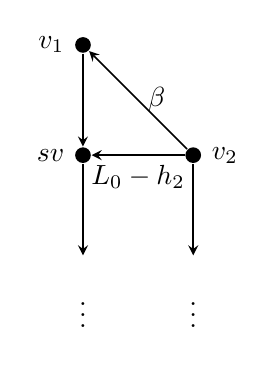
\begin{tikzpicture}
[->, node distance = 1.4cm,>=stealth,semithick]
\node[sv, label = left:{$v_1$}] (1) {};
\node[sv, label=left:{$sv$}] [below of =1] (2) {};
\node[sv, label=right:{$v_2$}] [right of =2] (3) {};
\node[label={below:$\vdots$}] [below of =2] (4) {}; 
\node[label={below:$\vdots$}] [below of =3] (5) {}; 
\path{
(1) edge (2)
(3) edge node [below]{$L_0 -h_2$} (2)
(3) edge node [right] {$\beta$} (1)
(2) edge (4)
(3) edge (5)
};
\end{tikzpicture}
}
\end{center}
\caption{A Jordan block between two highest weight modules creates what is known as a staggered module. Here $v_1$ and $v_2$ are two highest weight vectors with $sv$ a singular vector in the module obtained from $v_1$.  The  scalar $\beta$  uniquely determines the staggered module.}\label{fig:StagTri}
\end{figure}

The key finding from \cite{RidStag09}, was that each staggered module sits inside a 1-parameter family of modules, there is then a canonical way of uniquely determining this parameter referred to as $\beta$. Referring to figure \ref{fig:StagTri}, normalise $v_1$ such that coefficient of the $L_{-1}^n$ term in the singular vector is one. Then apply the adjoint of the singular vector monomials to $v_2$. This should return a scalar multiple of $v_1$. The scalar is $\beta$.\\ 

The question can then be proposed: How does this all work in the Neveu-Schwarz sector of the $N=1$ super Virasoro algebra? It is expected to behave in a very similar fashion due to the similarity in algebras. The more challenging case is that of the Ramond sector. Here the expected structures are not clear and detailed investigation will offer insight into more general logarithmic structures in the $N>1$ cases. \\

It is also possible to obtain fusion products via lattice calculations in statistical mechanics \cite{PeaRasLog06,ReaAss07}. Here the eigenvalues of $L_0$ are obtained through diagrammatic means and numerical approximation \cite{CarInv86}. Given this physical motivation, we set about the task through a process of explicit calculation of interesting fusion products to ascertain the resulting structure and classification.\\

In chapter 1, I cover the preliminary material on Verma modules through the example of the Virasoro algebra. Here the basic tenets of conformal field theory are presented. I develop the theory through a blend of the language of vertex algebras and the physical notation found in \cite{MatCFT97}. The goal is to briefly outline the key elements when considering minimal models, the representation theory, the modular transformations of characters and the fusion rules for the logarithmic analogue to come.\\

In chapter 2, I build on the Virasoro theory with the $N=1$ superconformal algebra representation theory. Here we extend the Kac table to include an infinite number of representations of the Neveu-Schwarz and Ramond algebra that will allow for logarithmic coupling in the following chapters. The representation theory of the Neveu-Schwarz algebra mirrors that of the Virasoro algebra where as that of the Ramond algebra is a little more complicated due to the presence of a $G_0$-operator. The structures of interest are certain submodules of Fock spaces known as Kac modules. \\

In chapter 3, I outline one of the main tools of this analysis, the fermionic Verlinde formula. As we are considering an infinite number of representations, we require a continuous analogue of the Verlinde formula. We construct the fermionic Verlinde formula from its bosonic counterpart and establish the Grothendieck fusion ring of characters and supercharacters for the Kac modules.\\

In chapter 4, I introduce the fundamental tool of this analysis, the Nahm-Gaberdiel-Kausch coproduct formulae. An explicit fusion product of Kac modules is calculated using the Nahm-Gaberdiel-Kausch algorithm. The fusion product of a \ram{} representation with a \ns{} representation or two \ram{} representations requires an adapted version of the usual Nahm-Gaberdiel-Kausch algorithm, which brings with it a certain level of variability through the introduction of twist parameters. We show that only a finite set of twist parameters allow for a meaningful result of the fusion product when using this algorithm.\\

In chapter 5, I then discuss the results of this analysis and offer some conjectures on the structure and patterns to be found. The results reveal Jordan blocks in the expected places when compared to the Virasoro case along with indecomposability parameters to determine the structure.\\

Appendix A, provides a derivation of the Nahm-Gaberdiel-Kausch algorithm. Appendix B, introduces the concept of a staggered module, the main structure of interest found when the fusion product of two representations contain a Jordan block. Appendix C, contains a table of results of fusion products found from combining the algorithm with the fermionic Verlinde formula and theory of staggered modules. Appendix D, contains a flow diagram of the programmatic implementation of the Nahm-Gaberdiel-Kausch algorithm.


\chapter{Virasoro Representation Theory}

In this chapter we will use the familiar example of the Virasoro algebra to elucidate the concepts in representation theory and conformal field theory necessary to the remainder of this thesis. The remainder of this thesis will focus on the super Virasoro algebra where in addition to the generating function of Virasoro modes we also have an additional set of fermionic modes. The super Virasoro algebra has similar representation theory to the Virasoro case with a few key distinctions that will be examined in the next chapter. 

The primary source for this material will be the texts \cite{MatCFT97, FrenkVert01}. We cover the highest weight representation theory of the Virasoro algebra and its vertex operator algebra as well as the conformal field theory concepts of minimal models, fusion, the Verlinde formula and finally logarithmic minimal models. Fusion will be examined via the usual method of correlation functions in this chapter, however we will see later how this may be done algebraically and algorithmically via the Nahm Gaberdiel Kausch algorithm, where fusion is considered to be the tensor product of vertex operator algebra representations. In this chapter we see the bosonic Verlinde formula which will be of importance when considering the Verlinde formula in the fermionic setting. We also show how logarithmic conformal field theory may be seen as the study of indecomposable representations of the Virasoro algebra.




\section{Verma Modules}

The Virasoro algebra is the complex vector space spanned by Virasoro modes $L_n$ and central element $C$ satisfying the Lie bracket relations
\begin{align*}
[L_m, L_n] &= (m-n) L_{m+n} + \frac{m^3 - m}{12} \delta_{m,-n}C & [L_m, C] = 0&& m,n\in \Z
\end{align*}

The algebra admits a triangular decomposition, split by mode index into negative, zero and positive components.
\begin{align*}
\mathfrak{vir} = \mathfrak{vir}^- \oplus \mathfrak{vir}^0 \oplus \mathfrak{vir}^+
\end{align*}

We will consider modules over the universal enveloping algebra $\mathcal{U}$ of this algebra. We may treat this as the associative unital algebra freely generated by Virasoro modes subject to the Lie bracket relations, where the Lie bracket may now be regarded as the commutator $[L_m,L_n] = L_mL_n - L_nL_m$. Once again we impose a triangular decomposition into finite length products of negative, zero and positive modes which we will denote by $\mathcal{U}^-, \mathcal{U}^0, \mathcal{U}^+$. Note that $\mathcal{U}$ becomes a Virasoro module under left multiplication. 
To construct a Verma module, we begin by defining a one dimensional representation $\rho$, of $\mathcal{U}^{\ge 0}$ (the subalgebra generated by non-negative Virasoro modes) over a vector space $\C v$. The {\bf highest weight vector} $v_{h,c}$ is simultaneously an eigenvector of $L_0$ and $C$, with respective eigenvalues ({\bf conformal weight}) $h$ and $c$.
\begin{align}
\rho(L_0) .v_{h,c} & = hv_{h,c}&\rho(C).v_{h,c} &= cv_{h,c}&\rho(L_n).v_{h,c} &= 0&n>0 \label{eqn:hwv}
\end{align}

The subalgebra $\mathcal{U}^+$ annihilates the highest weight vector. The Verma module then follows from the induced module construction whereby $\mathcal{U}^-$ ({\bf the creation operators}) acts freely on the highest weight vector.

\begin{defn}
The {\bf Verma module} of the Virasoro algebra with conformal weight $h$ and central charge $c$ is the induced module
\begin{align*}
\mathcal{V}_{h,c} = \mathcal{U}\otimes_{\mathcal{U}^{\ge 0}} \C v_{h,c}
\end{align*}
\end{defn}

By the Poincare-Birkhoff-Witt theorem this module admits a basis in which the Virasoro modes are ordered by mode index \cite{BirRep37}.

\begin{thm}
A basis for the universal enveloping algebra of $\mathfrak{vir}$ is given by
\begin{align*}
\{L_{-n_1}\dots L_{-n_k}|n_1\ge n_2 \ge\dots \ge n_k\}
\end{align*}
and thus a basis for $\mathcal{V}_{h,c}$ is given by
\begin{align*}
\{L_{-n_1}\dots L_{-n_k}v_{h,c}|n_1\ge \dots \ge n_k \ge 1\}
\end{align*}
\end{thm}

Each basis state is then an $L_0$ eigenvector of eigenvalue $h + \sum_i n_i$. As a result $\mathcal{V}_{h,c}$ admits a $\Z$-grading under $L_0$. 
\begin{align*}
\mathcal{V}_{h,c} = \bigoplus_{n\in \Z} \mathcal{V}_{h,c}^n
\end{align*}

The dimension of each $\mathcal{V}_{h,c}^n$ is equal to the number of partitions of $n$ with basis given by  
\begin{align*}
\mathcal{B}_n = \{L_{-n_1}\dots L_{-n_k}v_{h,c}|n_1\ge \dots \ge n_k \ge 1, \sum_i n_i = n\}
\end{align*}

Verma modules are completely parametrised by conformal weight $h$ and central charge $c$. We detail the submodule structure of $\mathcal{V}_{h,c}$. A Verma submodule, itself being a Verma module, is generated by {\bf singular vectors} \cite{FeiFuch90} satisfying the properties of (\ref{eqn:hwv}). Due to the fact $L_1$ and $L_2$ generate $\mathcal{U}^+$, singular vectors may be found by solving the set of equations
\begin{align*}
L_{1}\sum_{X_i\in \mathcal{B}_n} \alpha_i X_i  &= L_{2}\sum_{X_i\in \mathcal{B}_n} \alpha_i X_i  = 0
\end{align*}

We are interested in the set of conformal weights for which a solution to the above exists for a fixed value of central charge. We begin by placing a bilinear form on the module $\bra \cdot,\cdot \ket$ normalised by $\bra v_{h,c},v_{h,c}\ket =1$ with adjoint operation $L_{-n}^+ = L_n$. This then defines a scalar product under which singular vectors belong to the kernel $\bra \chi,w \ket=0$ $ \forall w\in U^- v_{h,c}$. Let $\chi$ be a singular vector in $\mathcal{V}_{h,c}$ with $\chi=U^-v_{h,c} $ for $U^-\in \mathcal{U}^-$. Then it can be seen that
\begin{align*}
\bra \chi, w \ket = \bra \chi, U^-v_{h,c} \ket = \bra U^+\chi, v_{h,c} \ket = 0
\end{align*}
Where $U^+$ is the adjoint of $U^-$. As such we are able to locate singular vectors by finding vectors in the kernel of the bilinear form. We fix the central charge and analyse the module for fixed grade. A finite set of conformal weights will then lead to zero norm states at this grade. We show this explicitly in the following example. 

\begin{exmp}
Consider a Virasoro Verma module of highest weight $h$. The level 2 basis states are $\{L_{-1}^2v, L_{-2}v\}$. We construct a matrix of scalar products ({\bf Gram matrix}).
\[
M^{(2)} = 
\begin{pmatrix}
\bra L_{-1}^2v, L_{-1}^2v\ket & \bra L_{-1}^2v, L_{-2}v\ket \\
\bra L_{-2}v, L_{-1}^2v \ket & \bra L_{-2}v, L_{-2}v\ket
\end{pmatrix}
=
\begin{pmatrix}
4h(2h+1) & 6h \\
6h & 4h + c/2
\end{pmatrix}
\]
Then there exists a singular vector at level 2 if this matrix has zero eigenvalue for some value of $h$. The matrix has determinant
\begin{align*}
\text{det} M^{(2)} &= 32(h-h_{1,1})(h-h_{1,2})(h -h_{2,1})\\
h_{1,1}&=0\\
h_{1,2}(c)& = \frac{1}{16}(5-c-\sqrt{(1-c)(25-c)})\\
h_{2,1}(c)& = \frac{1}{16}(5-c+\sqrt{(1-c)(25-c)})
\end{align*}
Then for any given central charge $c$ the Verma modules $\mathcal{V}_{h_{1,2}(c)}$ and $\mathcal{V}_{h_{2,1}(c)}$ will each contain a singular vector at level 2. We ignore the module $\mathcal{V}_{h_{1,1}(c)}$ as the level 2 state in the kernel of the scalar product here is actually a descendant of its level 1 singular vector $L_{-1}v$. 
\end{exmp}

A general formula for the determinant of a Gram matrix was first conjectured by Kac \cite{KacContForm79} and proved by Feigin-Fuchs \cite{FeiVerm83}. 
\begin{align*}
\text{det} M^{(l)} &= \text{Const} \times \prod_{\substack{r,s \ge 1 \\ rs\le l}} [h - h_{r,s} (t)]^{p(l-rs)}\\
h_{r,s}(t)  &= \frac{r^2 - 1}{4}t - \frac{rs-1}{2} + \frac{s^2-1}{4}t^{-1}\\
c(t) = 13 - 6\left(t+t^(-1)\right)
\end{align*}
Where $p(n)$ is the number of partitions of $n$ and $t\in \C$ is invariant under $t\leftrightarrow t^{-1}$. 

\begin{align*}
\text{det} M^{(1)} &=  (h-h_{1,1})\\
\text{det} M^{(2)} &=  (h-h_{1,1})(h-h_{1,2})(h-h_{2,1})\\
\text{det} M^{(3)} &=  (h-h_{1,1})^2(h-h_{1,2})(h-h_{2,1})(h-h_{1,3})(h-h_{3,1})\\
\vdots
\end{align*}

We can see from the above that $h_{r,s}$ as a root at $l=rs$, as $p(l-rs) = 0$ for $l<rs$. It then follows that a singular vector is found at level $rs$ or less in the module $V_{h_{r,s}(c)}$. It is the Jantzen filtration that confirms a singular vector at level $rs$ \cite{AstStr97}. As the singular vector generates a Verma module, we expect to find $p(l-rs)$ descendant states at level $l$ in the kernel of the scalar product. The above determinant formula is crucial in the classification of Verma modules.

We describe here the four structure types for Virasoro Verma modules and present them in figure~\ref{fig:VirVermaStructures}.

\noindent{\bf Point} If $h\neq h_{r,s}(t)$ for any $r,s \ge 1$ then $\mathcal{V}_{h_{r,s}(c)}$ will be irreducible.\\
{\bf Link} If $t$ is irrational we see that $h_{r,s}(t)\neq h_{r',s'}(t)$ for $(r,s)\neq (r',s')$ and as such $\mathcal{V}_{h_{r,s}(c)}$ contains a maximal irreducible submodule at grade $rs$.\\

When $t=\frac{p}{q}$ is rational we have an infinite set of nested submodules which we can further divide into two types. Central charge and conformal dimension are as follows
\begin{align*}
c &= 1-6\frac{(p-q)^2}{pq} \\
h_{r,s} &= \frac{(pr-qs)^2 - (p-q)^2}{4pq} 
\end{align*}
We are able to see that $V_{h_{r,s}(c)}$ will have a submodule at grade $rs$. We will restrict to $t$ positive, rational.   The set of weights for which $0<r<q$ and $0<s<p$ constitute the {\bf Kac table}, whereby each representation has a {\bf Braid} structure of submodules. The set of weights for which either $r=mq$ or $s=np$ are boundary representations having a {\bf Chain} structure of submodules. The representations outside of the Kac table for which $p \nmid r$ and $q \nmid s$ are also braided.



\begin{figure}
\scalebox{0.7}{
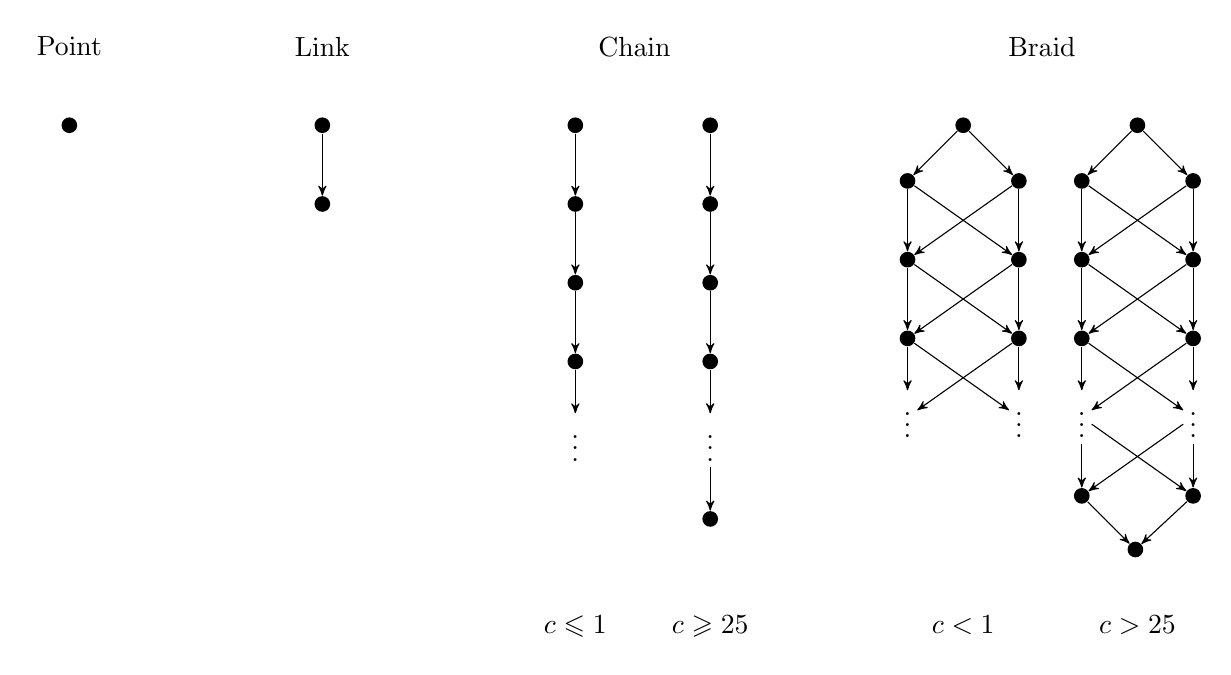
\begin{tikzpicture}[->,>=stealth', node distance=1cm]

  \node[main node] (1) [] {};
  \node[] (point) [above of =1] {Point};

  \node[main node] (2) [right = 3cm of 1] {};
  \node[] (link) [above of =2] {Link};
  \node[main node] (2a) [below of = 2] {};
  \path[]
  (2) edge node {} (2a);

  \node[main node] (3) [right = 3cm of 2] {};
  \node[] (chain) [right = 0.75cm of 3,above of =3] {Chain};
  \node[main node] (3a) [below of =3] {};
  \node[main node] (3b) [below of =3a] {};
  \node[main node] (3c) [below of =3b] {};
  \node[inner sep = 2pt] (3d) [below of =3c] {$\vdots$};

  \node[] (3bot) [below =6cm of 3] {$c \le 1$};

  \path[]
  (3) edge node {} (3a)
  (3a) edge node {} (3b)
  (3b) edge node {} (3c)
  (3c) edge node {} (3d);

  \node[main node] (4) [right = 1.5cm of 3] {};
  \node[main node] (4a) [below of =4] {};
  \node[main node] (4b) [below of =4a] {};
  \node[main node] (4c) [below of =4b] {};
  \node[inner sep = 2pt] (4d) [below of =4c] {$\vdots$};
  \node[main node] (4e) [below of =4d] {};

  \node[] (4bot) [below =6cm of 4] {$c \ge 25$};

  \path[]
  (4) edge node {} (4a)
  (4a) edge node {} (4b)
  (4b) edge node {} (4c)
  (4c) edge node {} (4d)
  (4d) edge node {} (4e);	

  \node[main node] (5) [right = 3cm of 4] {};
  \node[] (braid) [right = 1cm of 5,above of =5] {Braid};
  \node[main node] (5a) [below left of =5] {};
  \node[main node] (5b) [below of =5a] {};
  \node[main node] (5c) [below of =5b] {};
  \node[inner sep = 2pt] (5d) [below of =5c] {$\vdots$};

  \node[main node] (5e) [below right of =5] {};
  \node[main node] (5f) [below of =5e] {};
  \node[main node] (5g) [below of =5f] {};
  \node[inner sep = 2pt] (5h) [below of =5g] {$\vdots$};

  \node[] (5bot) [below =6cm of 5] {$c < 1$};

  \path[]
  (5) edge node {} (5a)
  (5a) edge node {} (5b)
  (5a) edge node {} (5f)
  (5b) edge node {} (5c)
  (5b) edge node {} (5g)
  (5c) edge node {} (5d)
  (5c) edge node {} (5h)
 
  (5) edge node {} (5e)
  (5e) edge node {} (5f)
  (5e) edge node {} (5b)
  (5f) edge node {} (5g)
  (5f) edge node {} (5c)
  (5g) edge node {} (5h)
  (5g) edge node {} (5d);	

  \node[main node] (6) [right = 2cm of 5] {};
  \node[main node] (6a) [below left of =6] {};
  \node[main node] (6b) [below of =6a] {};
  \node[main node] (6c) [below of =6b] {};
  \node[inner sep = 2pt] (6d) [below of =6c] {$\vdots$};
  \node[main node] (6d1) [below of =6d] {};

  \node[main node] (6d2) [below right = 0.75cm of 6d1] {};

  \node[main node] (6e) [below right of =6] {};
  \node[main node] (6f) [below of =6e] {};
  \node[main node] (6g) [below of =6f] {};
  \node[inner sep = 2pt] (6h) [below of =6g] {$\vdots$};
  \node[main node] (6h1) [below of =6h] {};

  \node[] (6bot) [below =6cm of 6] {$c > 25$};

  \path[]
  (6) edge node {} (6a)
  (6a) edge node {} (6b)
  (6a) edge node {} (6f)
  (6b) edge node {} (6c)
  (6b) edge node {} (6g)
  (6c) edge node {} (6d)
  (6c) edge node {} (6h)
  (6d) edge node {} (6d1)
  (6d) edge node {} (6h1)
  (6d1) edge node {} (6d2)
 
  (6) edge node {} (6e)
  (6e) edge node {} (6f)
  (6e) edge node {} (6b)
  (6f) edge node {} (6g)
  (6f) edge node {} (6c)
  (6g) edge node {} (6h)
  (6g) edge node {} (6d)
  (6h) edge node {} (6h1)
  (6h) edge node {} (6d1)
  (6h1) edge node {} (6d2);	

\end{tikzpicture}
}
\caption{The \sv{} structure, marked by black circles, of Virasoro Verma modules.  Arrows from one \sv{} to another indicate that the latter may be obtained from the former by acting with a suitable linear combination of monomials in the $L_n$.  Note that $t > 0$ corresponds to $c \le 1$ and $t < 0$ corresponds to $c \ge 25$.} \label{fig:VirVermaStructures}
\end{figure}

%\begin{figure}
%\begin{center}
%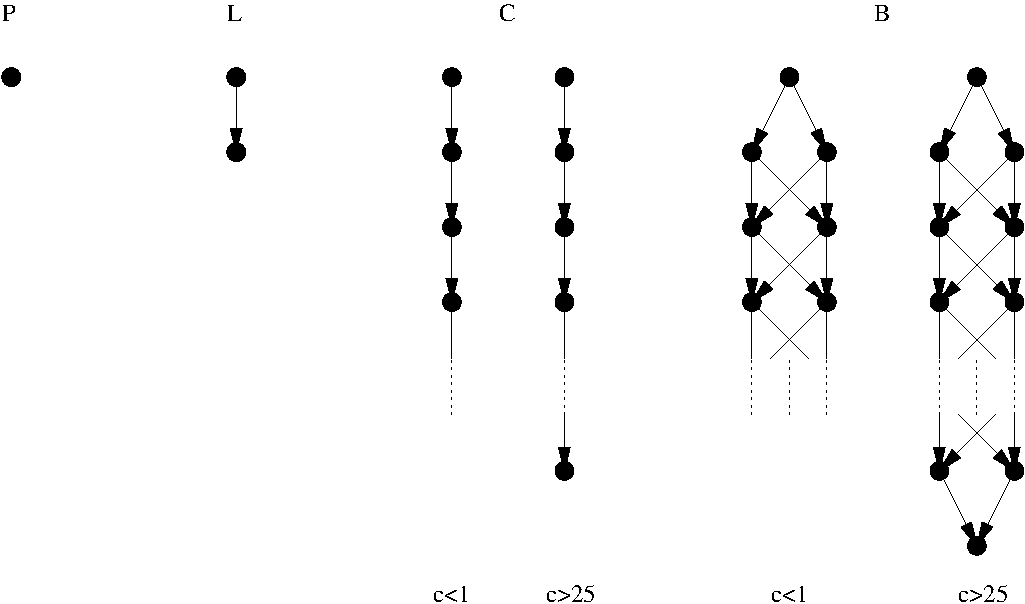
\includegraphics[scale=0.7]{NSMods}
%\end{center}
%\end{figure}

It is desirable to keep track of the dimension of each $L_0$ weight space $\mathcal{V}_{h_{r,s}(c)}^n$.

\begin{defn}
The {\bf character} of a Virasoro Verma module $\mathcal{V}_{h_{r,s}(c)}$, is the generating function
\begin{align*}
\text{ch}[\mathcal{V}_{h_{r,s}(c)}] = \sum_{n\in\Z_{\ge 0}} \text{dim}[\mathcal{V}_{h_{r,s}(c)}^n] q^{n+h-c/24}&&q=e^{2\pi i \tau}
\end{align*}
which can be expressed more succinctly through the use of the Dedekind eta function
\begin{align*}
\text{ch}[\mathcal{V}_{h_{r,s}(c)}](\tau) =\frac{q^{h+(1-c)/24}}{\eta(\tau)} 
\end{align*}
\end{defn}


%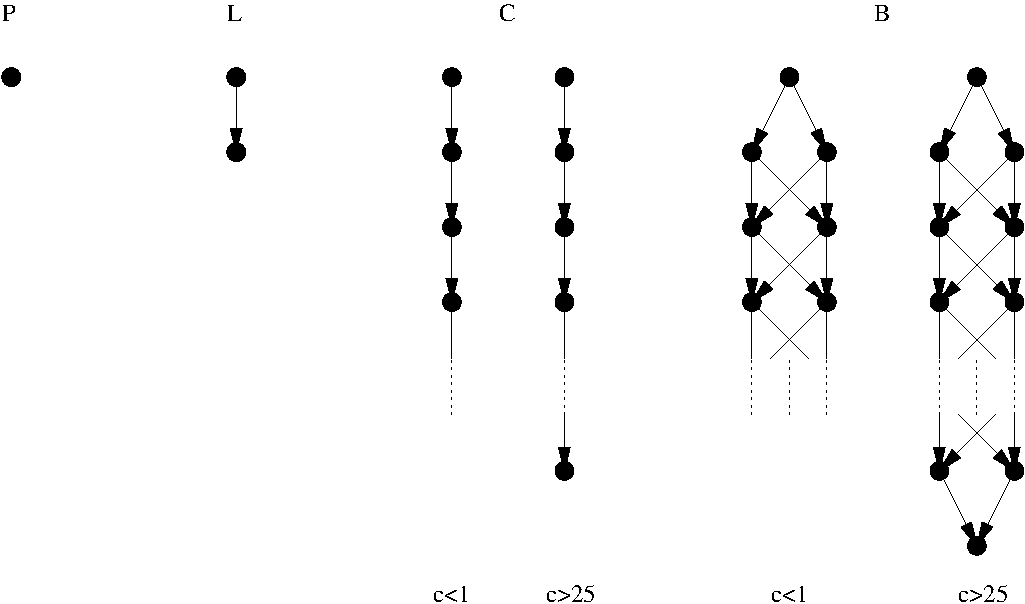
\includegraphics[scale=0.5]{NSMods}

\section{Vertex Operator Algebras}

The algebraic structure of relevance to the study of conformal field theory is not the Lie algebra but rather the vertex operator algebra.

\begin{defn}
A vertex algebra is a collection of data \cite{FrenkVert01}:

\begin{enumerate}
\item (space of states) A vector space V
\item (vacuum vector) A vector $|0\ket \in V$
\item (translation operator) A linear operator $D:V\rightarrow V$
\item (vertex operators) A linear operation
\begin{align*}
Y(\cdot, z):V\rightarrow \text{End}V[[z^{\pm 1}]]
\end{align*}
taking each $A\in V$ to a field
\begin{align*}
Y(A, z) = \sum_{n\in \Z} A_{(n)}z^{-n-1}
\end{align*}
where each  $A_{(n)}$ is a linear operator acting on $V$
\end{enumerate}
Along with the axioms
\begin{enumerate}
\item (vacuum axiom) $Y(|0\ket,z) = \text{Id}_V$ and $\lim_{z\rightarrow 0} Y(A,z)|0\ket = A$
\item (translation axiom) For all $A\in V$
\begin{align*}
[D,Y(A,z)] = \partial_z Y(A,z)
\end{align*}
and $D|0\ket=0$
\item (locality axiom) All fields are mutually locally, i.e. for all $A,B\in V$, there exists some $N\in \Z_{+}$ such that
\begin{align*}
(z-w)^N[Y(A,z), Y(B,w)] = 0
\end{align*}
\end{enumerate}

For the vertex algebra to be considered conformal and so be referred to as a vertex operator algebra, we also require the existence of $T(z)$,
\begin{align*}
T(z) = \sum_{n\in \Z} L_nz^{-n-2}
\end{align*}
such that the $L_n$ generate a copy of $\mathfrak{vir}$ and $D=L_{-1}$. $\omega = L_{-2}|0\ket$ is called the conformal vector.
\end{defn}




\begin{exmp} In the Virasoro case the vector space $V$ is generically the quotient of the $h=0$ Verma module by the submodule generated by the singular vector $L_{-1}|0\rangle$. This gives the universal vertex operator algebra. The translation operator is then the Virasoro mode $L_{-1}$ and the vertex operators are given by 
\begin{align*}
Y(L_{j_1}\dots L_{j_m}v_c,z) = \frac{1}{(-j_1-2)!}\dots\frac{1}{(-j_m-2)!}:\partial_z^{-j_1-2}T(z)\dots\partial_{z}^{-j_m-2}T(z):
\end{align*}
for $j_r\le-2$.
\end{exmp}

We are interested in the products of these fields (vertex operators). This is known as the {\bf operator product expansion}. We show here the example of the operator product expansion of $T(z)$ with itself where we implement the vacuum axiom and state-field correspondence. We begin with the ansatz
\begin{align*}
T(z)T(w) &= \sum_{m\in \Z} \psi_m (w)(z-w)^{-m-2}
\end{align*}
If we apply the vacuum to both sides and take the limit as $w\rightarrow 0$
\begin{align*}
\sum_{n\in \Z} L_n L_{-2}|0\ket z^{-n-2}&= \sum_{m\in \Z} |\psi_m\ket z^{-m-2}
\end{align*}
\begin{align*}
T(z)T(w) &= \frac{Y(L_2L_{-2}|0\ket, w)}{(z-w)^4}+ \frac{Y(L_0L_{-2}|0\ket, w)}{(z-w)^2} + \frac{Y(L_{-1}L_{-2}|0\ket, w)}{(z-w)}+ \dots\\
& = \frac{c/2}{(z-w)^4} + \frac{T(w)}{(z-w)^2} + \frac{\partial T(w)}{(z-w)} + \dots
\end{align*}

\section{Vertex Operator Algebra Representations}

We are interested in determining the set of Virasoro vertex algebra representations corresponding to a central charge. Here we will show the case $c=-22/5$ ($t=\frac{2}{5}$).

\begin{defn}
A vertex operator algebra representation is a vector space $M$ and an action $Y^M:V\otimes M\rightarrow M((z))$ satisfying the following:

\begin{enumerate}
\item (Identity) $Y^M(|0\ket,z) = \text{Id}_M$
\item (Locality) All fields $Y^M(A,z)$ are mutually local
\end{enumerate}

\end{defn}

If we consider the requirement that our representations are simple conformal vertex algebra representations, then they should respect the relations of the conformal vertex algebra. In this case, our vector space $M$ is a vacuum module. This will lead to a smaller set of representations than the universal vertex algebra. In forming the vacuum module we set the following singular vector to zero. Such a vector is known as a {\bf null vector},
\begin{align*}
\mathcal{N} = (L_{-4} - \frac{5}{3}L_{-2}^2)|0\ket
\end{align*}
a vector which we set to zero in the quotient VOA. The null field corresponding to this state is given by
\begin{align*}
\mathcal{N}(z) =  Y( L_{-4} - \frac{5}{3}L_{-2}^2, z) = \frac{1}{2}\partial_z^2 T(z) - \frac{5}{3}:T(z)T(z): 
\end{align*}

When we quotient out by this submodule in the vacuum module, we expect the VOA to respect this structure and hence it follows that the null field should then act as the zero operator by the state-field correspondence. We consider the action of the zeroth mode of this field on an arbitrary highest weight state $|h\ket$ to derive a constraint on the set of possible conformal weights $h$.
\begin{align*}
\mathcal{N}(z)_0 &= \frac{1}{2}\partial_z^2 T(z)_0 - \frac{5}{3}:T(z)T(z):_0 \\
& = \sum_{r\in \Z} :L_r L_{-r}: - \frac{9}{5}L_0\\
\end{align*}

The normal ordering for Virasoro modes is as follows.

\[
:L_mL_n: = \begin{cases}L_m L_n&m\le -2\\ L_n L_m & m \ge -1  \end{cases}
\]

\begin{align*}
\mathcal{N}(z)_0 &= 2\sum_{r\ge 2} L_{-r} L_{r} + L_{-1}L_{1} + L_{1}L_{-1} + L_0^2  - \frac{9}{5}L_0\\
\end{align*}

Acting on the highest weight state
\begin{align*}
\mathcal{N}(z)_0 |h\ket &= \left(L_{1}L_{-1} + L_0^2  - \frac{9}{5}L_0\right) |h\ket\\
& = \left(2L_0 + L_0^2  - \frac{9}{5}L_0\right) |h\ket\\
& = \left(\frac{1}{5}h + h^2\right)|h\ket = 0
\end{align*}


The suitable conformal weights are then $h= 0,-\frac{1}{5}$. We see that this is in accordance with the Kac table conformal weights
\begin{align*}
h_{r,s} = \frac{(pr-qs)^2-(p-q)^2}{4pq}&&1\le r < q&& 1\le s <p
\end{align*}
for $p=2$ and $q=5$. 

We are interested in relaxing the above condition that $\mathcal{N}$ be null. Doing so allows for a wider class of representations whereby we are no longer restricted to the minimal model conformal weights $h=0,-1/5$ but rather the logarithmic minimal model (to be explained later).

\section{Minimal Models}

\begin{defn}
For each positive rational value of $t=\frac{p}{q}$, we have a non-empty set of conformal weights $\{h_{r,s}| r<q , s<p\}$, where each weight corresponds to an irreducible representation. These are known as the {\bf minimal models} and will be denoted by $M(p,q)$.
\end{defn}

 \begin{exmp}
 The minimal model $M(4,5)$ has central charge $\frac{7}{10}$ and Kac table

\begin{table}[H]\label{tab:M45Kac}
\doublespacing
\[
\begin{tabular}{ >{$}l<{$} | >{$}c<{$} >{$}c<{$}  >{$}c<{$}  >{$}r<{$} }
   & 1 & 2 & 3 & 4 \\ \hline
  1 & 0 & \tfrac{1}{10} & \tfrac{3}{5} & \tfrac{3}{2} \\
  2 & \tfrac{7}{16} & \tfrac{3}{80} & \tfrac{3}{80} & \tfrac{7}{16} \\
  3 & \tfrac{3}{2} & \tfrac{3}{5} & \tfrac{1}{10} & 0 \\
\end{tabular}
\]
\end{table}

\end{exmp}

Each minimal model representation is irreducible and has an associated character which may be calculated by considering the appropriate addition and subtraction of characters of Verma submodules in a Virasoro Verma module. We give here the formula \cite{MatCFT97}

\begin{align*}
\chi_{(r,s)}(q) = \frac{q^{-c/24}}{\phi(q)}\left[q^{h_{r,s}} + \sum_{k=1}^{\infty}(-1)^k\left(q^{h_{r+kp',(-1)^k s+[1-(-1)^k]p/2}}+q^{h_{r,kp+(-1)^ks+[1-(-1)^k]p/2}}\right)\right]
\end{align*}

In the previous section, if we were to relax the condition that $\mathcal{N}$ be null, we would instead be left with the universal vertex algebra. The set of representations associated to the universal vertex algebra comprise the logarithmic minimal models.

\begin{defn}
For each positive rational value of $t=\frac{p}{q}$, we have a non-empty set of conformal weights $\{h_{r,s}| r\ge 1 , s\ge 1\}$. These are known as the {\bf logarithmic minimal models} and will be denoted by $M(p,q)$.
\end{defn}

The representation theory for logarithmic minimal models is more involved and will be described in detail in the following chapter.

\section{Fusion}

We introduce here the notion of a {\bf primary field} \cite{MatCFT97}. In the previous example we illustrated the state field correspondence for the Virasoro algebra. Fields corresponding to highest weight states are known as {\bf primary fields}. Fields corresponding to descendant states are appropriately named {\bf descendant fields}.\\

In the previous examples we calculated the product of the field $T(z)$ with itself. Likewise, we can calculate the product of $T(z)$ with a primary field and furthermore the associated {\bf correlation function}.

\begin{defn}
Given a set $A_1, A_2, \dots , A_n \in V$ and $\varphi \in V^*, v\in V$, the formal power series in $\C[[z^{\pm 1}, \dots z_n^{\pm 1}]]$ of primary fields
\begin{align*}
\bra \varphi, Y(A_1, z_1)\dots Y(A_n, z_n)v\ket
\end{align*}
are called the n-point {\bf correlation functions}
\end{defn}

 A weaker goal than calculating the correlation function of all the primary fields is to calculate their {\bf fusion products}. 
 
 \begin{defn}
The fusion product of $Y(A_1,z_1)$ with $Y(A_2,z_2)$ is the set of all primary fields $Y(A_n, z_n)$ for which the correlation function,
\begin{align*}
\bra \varphi, Y(A_1,z_1)Y(A_2,z_2)Y(A_n,z_n) v\ket
\end{align*}
is non-zero. 
\end{defn}

We can then notate this compactly by,
\begin{align*}
[A_1]\times [A_2] = [A_3] + \dots
\end{align*}
where $[A]$ corresponds to the highest weight representation with highest weight state $A$.

Then by associativity we are able to calculate fusion products with more terms. It is the central goal of conformal field theory to calculate these products. We demonstrate the calculation for a case in the Virasoro sector when $c=0$.\\

\begin{exmp}
For $c=0$ the singular vector at depth $2$ for the representation $h_{1,2}$ over the universal vertex algebra, is given by
\begin{align*}
\chi = (L_{-1}^2 - \frac{2}{3}L_{-2})|h_{1,2}\ket
\end{align*}

We will show the following fusion product,
\begin{align}
[h_{1,2}] \times [h_{r,s}] = [h_{r,s-1}] + [h_{r,s+1}] \label{eqn:h12frule}
\end{align}

To do so we first show how descendant fields correspond to differential operators in correlation functions. Let $Y(|h\ket,w)$ be the primary field corresponding to the highest weight state $|h\ket$. Let $Y(\chi,w)$ be the descendant field corresponding to the singular vector above. Then for two representations $[h_1]$ and $[h_2]$,
\begin{align}
0 &= \bra Y(\chi,w) Y(|h_{1}\ket,w) Y(|h_{2}\ket,w) \ket \\
  &= (\mathcal{L}_{-1}^2 - \frac{3}{2}\mathcal{L}_{-2}) \bra  Y(|h\ket,w) Y(|h_{1}\ket,w_1) Y(|h_{2}\ket,w_2) \ket \label{eqn:CorDE}
\end{align}
where
\begin{align*}
\mathcal{L}_{-n}  = \sum_i \left(\frac{(n-1)h_i}{(w_i-w)^n}-\frac{1}{(w_i-w)^{n-1}}\partial_{ w_i}\right)
\end{align*}
and the subscript $i$ refers to the remaining fields in the correlation function. To see this, consider the product of $T(z)$ with a primary field $Y(|h\ket,w)$,
\begin{align}\label{eqn:TPFope}
T(z)Y(|h\ket, w) &= \sum_{k\ge 0} (z-w)^{k-2} Y(L_{-k}|h\ket,w)\\
&= \frac{hY(|h\ket, w)}{(z-w)^2} + \frac{\partial Y(|h\ket, w)}{(z-w)} + \dots
\end{align}
Then we may rewrite the descendant field,
\begin{align*}
Y(L_{-n}|h\ket,w) = \oint_w (z-w)^{-n+1} T(z)Y(|h\ket,w) \, dz
\end{align*}
Then for a product of fields $X=\prod_{i=1}^n Y(|h_i\ket,w_i)$,
\begin{align*}
\bra Y(L_{-n}|h\ket,w) X \ket &= \frac{1}{2\pi i}\oint_w (z-w)^{-n+1}\bra T(z) Y(|h\ket, w) X \ket\\ 
&= -\frac{1}{2\pi i}\sum_i  \oint_{w_i} (z-w)^{-n+1}\left(\frac{h_i}{(z-w_i)^2} + \frac{\partial w_i}{(z-w_i)} \right) \bra Y(|h\ket, w) X \ket \, dz\\
& =  -\frac{1}{2\pi i}\sum_i  \oint_{w_i} \left( (-n+1) (w_i-w)^{-n+1}h_i +\right. 
\\ & \qquad \qquad \qquad  \left. (w_i-w)^{-n+1}\partial w_i \right) \bra Y(|h\ket, w) X \ket \, dz
\end{align*}
We then use the general form of the three-point correlation function \cite{MatCFT97}
\begin{align*}
\bra  Y(|h\ket,w) Y(|h_{1}\ket,w_1) Y(|h_{2}\ket,w_2) \ket = \frac{Const.}{(w-w_1)^{h+h_1-h_2}(w_1-w_2)^{h_1+h_2-h}(w-w_2)^{h+h_2-h_1}}
\end{align*}
to solve the differential equation (\ref{eqn:CorDE}). We then arrive at the constraints
\begin{align*}
h_2 = \frac{1}{6} + \frac{h}{3} + h_1 \pm \frac{2}{3} \sqrt{h^2 + 3hh_1 -\frac{1}{2}h + \frac{3}{2}h_1 + \frac{1}{16}}
\end{align*}
If we set $h = h_{1,2}$ and $h_1 = h_{r,s}$, then $h_2 \in \{h_{r,s-1},h_{r,s+1}\}$. We then arrive at the fusion rule given in (\ref{eqn:h12frule}).
\end{exmp}

We give here the fusion rules for minimal models
\begin{align*}
[h_{r,s}] \times [h_{m,n}] = \sum_{\substack{k=l+|r-m|\\ k+r+m=1 \bmod 2}}\sum_{\substack{l=1+|s-n|\\ k+s+n=1 \bmod 2}}[h_{k,l}]
\end{align*}

\section{Verlinde Formula}

In the previous section we give a method for calculating the fusion rules between representations in minimal models. It was conjectured in \cite{Ver88} that this may be found by consideration of modular transformations of the characters of these representations. The formula was shown to be true in \cite{MooCla89} and proven rigorously in \cite{HuaVer04}. The modular group $PSL(2;\mathbb{Z})$ has the generators

\begin{equation}
\mathcal{S} : \tau \rightarrow -\frac{1}{\tau} \qquad \qquad \mathcal{T} : \tau \rightarrow \tau + 1
\end{equation}

with relations

\begin{equation}
\langle S,T | S^2 = I, (ST)^3=I \rangle
\end{equation}
If we then take the $\mathcal{S}$-transformation of the minimal model characters $\chi_{r,s}(\tau)$, for a minimal model $M(p,p')$
\begin{align}
\mathcal{S}(\chi_{r,s}(\tau)) = 2\sqrt{\frac{2}{pp'}}\sum_{(p,\sigma)\in E_{p,p'}}(-1)^{1+s\rho+r\sigma}\sin(\pi \frac{p}{p'} r \rho) \sin(\pi \frac{p}{p'} s\sigma)\chi_{\rho,\sigma}(\tau)
\end{align}

where $E_{p,p'}$ is the set of tuples within the Kac table modulo the symmetry $ (r,s) \leftarrow \rightarrow (q-r,p-s)$. Then if the fusion of two representations $[h_{r,s}]$ and $[h_{m,n}] $ is expressed as the following sum
\begin{align}
[h_{r,s}]\times [h_{m,n}] = \sum_{(k,l)\in E_{p,p'}} \mathcal{N}_{(r,s)(m,n)}^{(k,l)} [h_{k,l}]
\end{align}

We are given the following famous formula for the fusion rules $\mathcal{N}_{(r,s)(m,n)}^{(k,l)}$, first given by Verlinde in \cite{Ver88}.
\begin{align}
\mathcal{N}_{(r,s)(m,n)}^{(k,l)} = \sum_{i=1}^{p'-1}\sum_{j=1}^{p-1}\frac{\mathcal{S}_{(r,s)}^{(i,j)}\mathcal{S}_{(m,n)}^{(i,j)}\mathcal{S}_{(i,j)}^{(k,l)}}{\mathcal{S}_{1,1}^{(i,j)}}
\end{align}

A goal of this thesis is to develop this Verlinde formula for the logarithmic setting.

\section{Logarithmic CFT}

The simplest of conformal field theories are comprised of irreducible representations of their infinite-dimensional symmetry algebra, with the Virasoro algebra being one example. There are however certain models from statistical mechanics and string theory that require indecomposable yet reducible representations. These models are then said to be examples of logarithmic conformal field theories as their correlation functions contain logarithmic singularities. We can think of these indecomposable representations as an $L_0$ action with a Jordan block. We would like to show the correspondence between an $L_0$ action containing a Jordan cell and logarithmic singularities in correlation functions first noted in a different way by Gurarie \cite{GurLog93}. The main reference for this section will be \cite{CreLog13}. We begin with the following $L_0$ matrix over an eigenvector $\phi$ and its Jordan partner, $\Phi$.

\[
L_0 = \begin{pmatrix}
h & 1\\
0 & h
\end{pmatrix}
\]

Our aim is to calculate the correlation function $\bra \Phi(z) \Phi(w) \ket$ and show the presence of logarithmic singularities. We will first need the commutation relations
\begin{align*}
[L_n, \Phi(w)] = \oint_w T(z)\Phi(w) z^{n+1} \frac{dz}{2\pi i}
\end{align*}

We calculate the operator product expansion of the stress energy tensor $T(z) = \sum_{m\in \Z} L_m z^{-m-2}$ with the vertex operator $\Phi(z)$. We begin with a Laurent expansion and solve for $\psi_n (z)$.
\begin{align*}
T(z)\Phi(w) = \sum_{n\in \Z}\psi_n (w) (z-w)^{-n-2}
\end{align*}

We apply the vacuum to both sides and take the limit $w \rightarrow 0$.
\begin{align*}
 \sum_{m\in \Z} L_m \Phi z^{-m-2} = \sum_{n\in \Z}\psi_n z^{-n-2}
\end{align*}

Returning to our ope, we now have the states of the Fourier coefficients.
\begin{align*}
T(z)\Phi(w) = \frac{(L_0 \Phi)(w)}{(z-w)^2} + \frac{(L_{-1} \Phi)(w)}{(z-w)} + \dots 
\end{align*}

It is at this point that the non-diagonal action of $L_0$ on $\Phi$ comes into play. Now using the state field correspondence we achieve the desired result.
\begin{align*}
T(z)\Phi(w) = \frac{h \Phi(w) + \phi(w)}{(z-w)^2} + \frac{\partial \Phi(w)}{(z-w)} + \dots 
\end{align*}

From which  we derive
\begin{align*}
[L_{-1}, \Phi(w)] &= \partial \Phi(w) \\
[L_0, \Phi(w)] &= h\Phi(w) + \phi(w)  + w\partial \Phi(w)\\
[L_1, \Phi(w)] &= hw\Phi(w) + w\phi(w)  + w^2\partial \Phi(w) 
\end{align*}

Applying the $L_{-1}$ operator to the correlation function
\begin{align*}
\bra L_{-1}\Phi(z)\Phi(w) \ket = (\partial_z + \partial_w)\bra \Phi(z)\Phi(w) \ket +  \bra \Phi(z)\Phi(w)L_{-1} \ket
\end{align*}

However both the term on the left hand side and final term on the right return zero as the vacuum is invariant under both $L_1$ and $L_{-1}$. We are thus left with the differential equation 
\begin{align*}
0 =  (\partial_z + \partial_w)\bra \Phi(z)\Phi(w) \ket 
\end{align*}

Repeating this process for the operators $L_0$ and $L_1$ and exchanging $\Phi$ with $\phi$ yields a set of differential equations which may then be solved to give the correlators
\begin{align*}
\bra \phi(z)\phi(w) \ket  &= 0\\
\bra \phi(z)\Phi(w) \ket  &= \frac{B}{(z-w)^{2h}}\\
\bra \Phi(z)\Phi(w) \ket &= \frac{C - 2B\log(z-w)}{(z-w)^{2h}}
\end{align*}

where $B$ and $C$ are constants. So we arrive at the mantra, Jordan blocks lead to logarithmic singularities. It is for this reason that we study indecomposable modules over the Virasoro and super Virasoro algebras with a non-diagonalisable $L_0$ action. We will see that the above treatment for minimal models may be adapted for the logarithmic case, whereby we  study the representation theory and show a novel new form of the Verlinde formula to understand the fusion rules of logarithmic minimal models.





\chapter{N=1 Representation Theory}

In this chapter we address the representation theory for the $N=1$ superconformal algebras. The super Virasoro algebra has wide ranging applications within mathematical physics, both in string theory and statistical mechanics. The algebra describes the infinitesimal symmetries of super strings as well as the continuum scaling limit of certain lattice models with integrable boundary conditions. Super conformal algebras contain $N$ fermionic fields, as such the $N=1$ super Virasoro algebra can be considered to be the simplest case right after the Virasoro algebra where $N=0$.
Within statistical mechanics there is a direct link between lattice diagrammatic methods and indecomposable representations of the Virasoro algebra. On the lattice the $L_0$ operator is modelled by the Hamiltonian after some constant shifts and rescalings. The key structure is the Kac module which we build towards by first introducing the $N=1$ Verma modules both in the Neveu Schwarz sector where the theory parallels that of the Virasoro and the Ramond sector where there are a few technicalities to consider owing to the presence of a nilpotent operator in the zero mode algebra. The Kac module is motivated by studies on the lattice, whereby certain character evaluations suggested a structure equivalent to a quotient of a Verma module is the relevant structure for these lattice calculations. We show that this is false following Virasoro papers \cite{RasCla11,MorKac14} and detail Kac module theory through a comprehensive picture of the  structures for three central charges.


\section{$\bm{N=1}$ algebras} \label{sec:Alg}

The $N=1$ superconformal algebras are infinite dimensional and may be defined as the vector spaces spanned by the bosonic modes, $L_n$ and $C$ and fermionic modes $G_k$ with the following bracket relations.

\begin{equation} \label{eq:CommN=1}
\begin{aligned}
\comm{L_m}{L_n} &= \brac{m-n} L_{m+n} + \frac{1}{12} \brac{m^3-m} \delta_{m+n=0} \, C, & \comm{L_m}{G_k} &= \brac{\frac{1}{2} m - k} G_{m+k}, \\
\acomm{G_j}{G_k} &= 2 L_{j+k} + \frac{1}{3} \brac{j^2-\frac{1}{4}} \delta_{j+k=0} \, C, & \comm{L_m}{C} &= \comm{G_j}{C} = 0.
\end{aligned}
\end{equation}
There are then two subalgebras which are distinguished by the values taken by the index $k$ of the fermionic modes $G_k$:  The \emph{\ns{} algebra} takes $k \in \ZZ + \frac{1}{2}$, whereas the \emph{Ramond algebra} takes $k \in \ZZ$.  Both algebras require the index $n$ of the bosonic modes $L_n$ to be an integer, hence the bosonic Lie subalgebra of each is identified with the Virasoro algebra.

The algebraic structures of interest to us are the universal vertex operator superalgebras associated to the \ns{} algebra. 
\begin{figure}[H]
\begin{center}
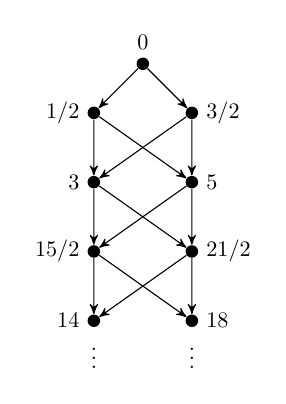
\begin{tikzpicture}[->,-stealth',scale=0.8, transform shape, node distance=1.1cm]
%
  \node[main node, label = above:$0$] (1) [] {};
%  \node[] (n) [above of =1] {$\Fock{1,1} = \Fock{3,5} = \cdots$};	
  \node[csv, label = left:1/2] (2) [below left of=1] {};
  \node[main node, label = right:3/2] (3) [below right of=1] {};
  \node[subsv, label = left:3] (4) [below of=2] {};
  \node[subsv, label = right:5] (5) [below of=3] {};
  \node[subsv, label = left:15/2] (7) [below of=4] {};
  \node[subsv, label = right:21/2] (6) [below of=5] {};
  \node[subsv, label = left:14, label = below:$\vdots$] (8) [below of=7] {};
  \node[subsv, label = right:18, label = below:$\vdots$] (9) [below of=6] {};
 \path[every node/.style={font=\sffamily\small}]
	(1) edge (2)
	(1) edge (3)
	(2) edge (4)
	(2) edge (5)
	(3) edge (4)
	(3) edge (5)
	(5) edge (6)
	(4) edge (6)
	(4) edge (7)
	(5) edge (7)
	(7) edge (8)
	(6) edge (8)
	(6) edge (9)
	(7) edge (9);
%
\end{tikzpicture}
\end{center}
\caption{Braided module structure for \ns{} sector when $p=2$ and $q=4$. Each dot represents a singular vector with a corresponding conformal weight given. An arrow from one singular vector to another indicates a descendant.} \label{fig:Kacc=0}
\end{figure}


If we consider the submodule structure of the Neveu Schwarz Verma module for $p=2$ and $q=4$ (see figure~\ref{fig:Kacc=0}) , then by the vacuum axiom we have that $G_{-1/2}|0\ket$ is necessarily zero, annihilating the weight $1/2$ singular vector and all of its descendants (i.e. the $3,5,15/2$ etc.), leaving us with the single singular vector of weight $3/2$

%\begin{figure}[H]
\begin{center}
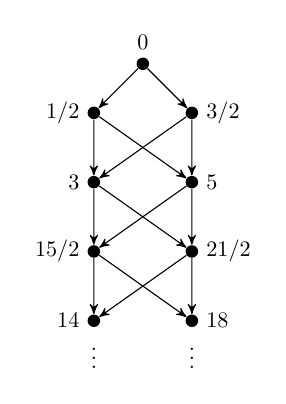
\begin{tikzpicture}[->,-stealth',scale=0.8, transform shape, node distance=1.1cm]
%
  \node[main node, label = above:$0$] (1) [] {};
%  \node[] (n) [above of =1] {$\Fock{1,1} = \Fock{3,5} = \cdots$};	
  \node[csv, label = left:1/2] (2) [below left of=1] {};
  \node[main node, label = right:3/2] (3) [below right of=1] {};
  \node[subsv, label = left:3] (4) [below of=2] {};
  \node[subsv, label = right:5] (5) [below of=3] {};
  \node[subsv, label = left:15/2] (7) [below of=4] {};
  \node[subsv, label = right:21/2] (6) [below of=5] {};
  \node[subsv, label = left:14, label = below:$\vdots$] (8) [below of=7] {};
  \node[subsv, label = right:18, label = below:$\vdots$] (9) [below of=6] {};
 \path[every node/.style={font=\sffamily\small}]
	(1) edge (2)
	(1) edge (3)
	(2) edge (4)
	(2) edge (5)
	(3) edge (4)
	(3) edge (5)
	(5) edge (6)
	(4) edge (6)
	(4) edge (7)
	(5) edge (7)
	(7) edge (8)
	(6) edge (8)
	(6) edge (9)
	(7) edge (9);
%
\end{tikzpicture}
\end{center}
\caption{Braided module structure for \ns{} sector when $p=2$ and $q=4$. Each dot represents a singular vector with a corresponding conformal weight given. An arrow from one singular vector to another indicates a descendant.} \label{fig:Kacc=0}
\end{figure}


\begin{center}
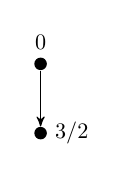
\begin{tikzpicture}[->,-stealth',scale=0.8, transform shape, node distance=1.1cm]
%
  \node[main node, label = above:$0$] (1) [] {};
%  \node[] (n) [above of =1] {$\Fock{1,1} = \Fock{3,5} = \cdots$};	
  \node[main node, label = right:3/2] (3) [below of=1] {};
 \path[every node/.style={font=\sffamily\small}]
	(1) edge (3);
%
\end{tikzpicture}
\end{center}

There are then two options here. If we were to set the weight $3/2$ singular vector to zero we would be left with an irreducible \ns{} vacuum module and an irreducible \ram{} module whose \hwv{} also has conformal weight $0$. If however we were to retain the weight $3/2$ singular vector then the set of representations becomes infinite and allows for a wider class of structures. This is known as the universal vertex operator algebra. We will be considering the latter case for the remainder of this thesis.  There are an infinite number of vertex operator superalgebras, parametrised by the central charge $c \in \CC$, and they are realised \cite{KacVer94} on the \ns{} module generated by a \hwv{} $\Omega$ satisfying
\begin{equation}
\begin{gathered}
L_0 \Omega = 0, \qquad C \, \Omega = c \, \Omega, \qquad G_{-1/2} \Omega = 0.\\
L_n \Omega = 0, \qquad G_k \Omega = 0 \qquad n,k > 0
\end{gathered}
\end{equation}

In other words, each such universal vertex operator superalgebra is defined on the quotient of the \ns{} Verma module $\NSVer{0}$, of conformal weight $0$ and central charge $c$, by the submodule generated by the \sv{} of conformal weight $\frac{1}{2}$ (see \cref{sec:Verma} below).  We will refer to these universal vertex operator superalgebras as the \emph{$N=1$ algebras}, for short.

Field-theoretically, each $N=1$ algebra extends the universal Virasoro vertex operator algebra (of the same central charge) by a fermionic primary field $G(z)$ of conformal weight $\frac{3}{2}$.  With the mode decompositions
\begin{equation} \label{eq:TGFourier}
T(z) = \sum_{n \in \ZZ} L_n z^{-n-2}, \qquad 
G(z) = \sum_{k \in \ZZ + \eps} G_k z^{-k-3/2},
\end{equation}
where $\eps = \frac{1}{2}$ in the \ns{} sector and $\eps = 0$ in the Ramond sector, the Lie brackets \eqref{eq:CommN=1} are equivalent to the \opes{}
\begin{equation} \label{OPE:TTTGGG}
\begin{gathered}
T(z) T(w) \sim \frac{c/2}{\brac{z-w}^4} + \frac{2 \, T(w)}{\brac{z-w}^2} + \frac{\pd T(w)}{z-w}, \\
T(z) G(w) \sim \frac{\frac{3}{2} \, G(w)}{\brac{z-w}^2} + \frac{\pd G(w}{z-w}, \qquad 
G(z) G(w) \sim \frac{2c/3}{\brac{z-w}^3} + \frac{2 \, T(w)}{z-w}.
\end{gathered}
\end{equation}
Note that the energy-momentum tensor and a Virasoro primary field are always mutually local (see \cite{RidLog07} for example):  $T(z) G(w) = G(w) T(z)$.  We emphasise that we have defined the $N=1$ algebra to be universal, meaning that the \opes{} \eqref{OPE:TTTGGG} generate a complete set of relations.  In particular, the $N=1$ algebra never coincides with an $N=1$ minimal model vertex operator superalgebra, even when $c$ is a minimal model central charge.
\begin{defn}
A {\bf conformal vertex superalgebra} is a vertex algebra satisfying the additional axioms
\begin{enumerate}
\item (superspace) $V$ admits the decomposition $V = V_{\bar{0}}\oplus V_{\bar{1}}$ with $|0\ket \in V_{\bar{0}}$
\item (parity preserving) For each $A\in V_{\bar{0}}$ all Fourier coefficients of $Y(A,z)$ should be parity preserving endomorphisms of $V$ and parity reversing for $A\in V_{\bar{1}}$. $T$ should have even parity.\\
Along with the replacement of the locality axiom by the following
\item (super locality)
\begin{align*}
(z-w)^N Y(A,z) Y(B,w) =(-1)^{p(A)p(B)} (z-w)^N Y(B,w) Y(A,z)
\end{align*}
for some $N\in Z_+$, where $p(A)$ denotes the parity of $A\in V$
\end{enumerate}
\end{defn}

\begin{exmp}
We construct the vertex algebra for the $N=1$ algebra. The translation operator is given by $L_{-1}$. We first construct the vacuum module. In the super Virasoro algebra the vacuum module is in the Neveu Schwarz sector for the reason that the module corresponding to the conformal weight $h_{1,1}=0$ and any central charge, contains a singular vector at a half integer grade (1/2). The Verma module is then obtained by applying all negative Neveu Schwarz modes to the vacuum vector. However the vacuum axiom reduces this space significantly. 
\begin{align*}
\lim_{z\to 0}Y(G_{-3/2}|0\ket, z)|0\ket &= \lim_{z\to 0}\sum_{m\in \Z} G_m|0\ket z^{-m-3/2}\\
&=\lim_{z\to 0}G_{-1/2}|0\ket z^{-1} + G_{-3/2}|0\ket 
\end{align*}
As such we are required to set $G_{-1/2}|0\ket$ to zero and subsequently all of its descendant states. Note that $G_{-1/2}|0\ket$ is a singular vector and the submodule it generates contains the $L_{-1}|0\ket$ vector. Then taking this quotient as our vacuum module $V$, we have the following state-field correspondence $Y(\cdot, z):V\rightarrow \text{End}V[[z^{\pm 1}]]$

\begin{center}
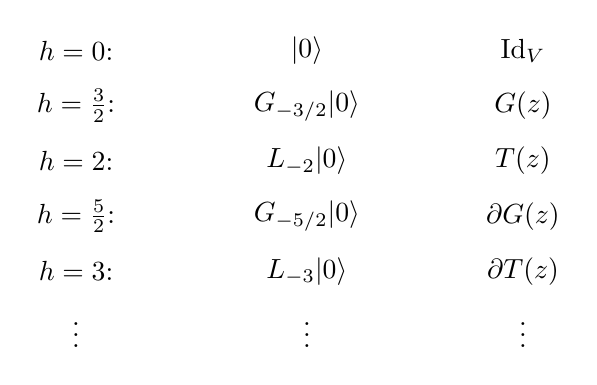
\begin{tikzpicture}
[node distance=0.7cm,>=stealth',semithick]
  \node[] (1) {$h=0$:};
  \node[] (1a) [below of=1] {$h=\tfrac{3}{2}$:};
  \node[] (1b) [below of=1a] {$h=2$:};
  \node[] (1c) [below of=1b] {$h=\tfrac{5}{2}$:};
  \node[] (1d) [below of=1c] {$h=3$:};
  \node[] (1e) [below of=1d] {$\vdots$};
%
  \node[] (2)   [right =2cm of 1] {$|0\ket$};
  \node[] (2a) [below of=2] {$G_{-3/2}|0\ket$};
  \node[] (2b) [below of=2a] {$L_{-2}|0\ket$};
  \node[] (2c) [below of=2b] {$G_{-5/2}|0\ket$};
  \node[] (2d) [below of=2c] {$L_{-3}|0\ket$};
  \node[] (2e) [below of=2d] {$\vdots$};
%
  \node[] (3)   [right =2cm of 2] {$\text{Id}_V$};
  \node[] (3a) [below of=3] {$G(z)$};
  \node[] (3b) [below of=3a] {$T(z)$};
  \node[] (3c) [below of=3b] {$\partial G(z)$};
  \node[] (3d) [below of=3c] {$\partial T(z)$};
  \node[] (3e) [below of=3d] {$\vdots$};
\end{tikzpicture}
\end{center}

In general this can be expressed as
\begin{align*}
Y(L_{j_1}\dots L_{j_n}G_{k_1}\dots G_{k_m}v_c,z) &= \frac{1}{(-j_1-2)!}\dots\frac{1}{(-j_n-2)!}:\partial_z^{-j_1-2}T(z)\dots\partial^{-j_n-2}T(z)\\
&\frac{1}{(-k_1-3/2)!}\dots\frac{1}{(-k_m-3/2)!}\partial_z^{-k_1-3/2}G(z)\dots\partial^{-k_m-3/2}G(z):
\end{align*}
with $j_r\le-2$ and $k_s\le -\frac{3}{2}$.\\
\end{exmp}


The category of modules over a given $N=1$ algebra is a full subcategory of the category of \ns{} modules consisting of the modules $\Mod{M}$ that satisfy the following conditions:  The central element $C$ acts on $\Mod{M}$ as $c$ times the identity operator and, for each $v \in \Mod{M}$, one has $L_n v = G_k v = 0$ for all sufficiently large $n$ and $k$.  The latter condition ensures that the orders of the poles in the \opes{} of $T(z)$ and $G(z)$ with $v(w)$, hence in those of every $N=1$ field with $v(w)$, are bounded above.  In what follows, we shall further restrict to modules that admit a $\ZZ_2$-grading compatible with that of the generators $L_n$ and $G_k$.  In other words, each $N=1$ module decomposes as a direct sum of two subspaces, one even and the other odd; each is preserved by the action of $L_n$ and they are swapped by the action of $G_k$.

For reasons of physical consistency, one is also led to consider the Ramond modules that satisfy the same conditions  Mathematically, Ramond modules are \emph{twisted} modules over the \ns{} algebra, hence over the $N=1$ algebra, though we will usually drop this qualifier in what follows and use the term \emph{$N=1$ module} to mean both \ns{} and Ramond modules.  We define the \emph{\ns{} sector} to consist of the $N=1$ modules that are \ns{} modules and the \emph{Ramond sector} to consist of the (twisted) $N=1$ modules that are Ramond modules.



\section{Extended Kac tables} \label{sec:KacTables}

The standard parametrisation suggested by the $N=1$ analogues \cite{KacCon79,FriSup85,MeuHig86} of the Kac determinant formula is
\begin{equation}
c = \frac{15}{2} - 3 \brac{t+t^{-1}}, \qquad 
h_{r,s} = \frac{r^2-1}{8} t^{-1} - \frac{rs-1}{4} + \frac{s^2-1}{8} t + \frac{1}{16} \delta_{r \neq s \bmod{2}},
\end{equation}
where $r,s \in \ZZ$ and $t \in \CC \setminus \set{0}$.  We remark that in applications to representation theory, the conformal weight $h_{r,s}$ is associated to a module in the \ns{} sector, when $r=s \bmod{2}$, and to a module in the Ramond sector, when $r \neq s \bmod{2}$.  If $t$ is rational, then this parametrisation may be written in the form
\begin{equation} \label{eq:ParByt}
t = \frac{p}{p'}, \qquad 
c = \frac{3}{2} \brac{1 - \frac{2 \brac{p'-p}^2}{pp'}}, \qquad 
h_{r,s} = \frac{\brac{p'r-ps}^2 - \brac{p'-p}^2}{8pp'} + \frac{1}{16} \delta_{r \neq s \bmod{2}},
\end{equation}
where one customarily imposes the constraints $p=p' \bmod{2}$ and $\gcd \set{p, \frac{1}{2} \brac{p'-p}} = 1$.

The $N=1$ superconformal minimal models \cite{EicMin85,BerSup85,FriSup85} correspond to $p,p' \in \ZZ_{\ge 2}$ satisfying these constraints. The indecomposable modules of the $N=1$ minimal model vertex operator superalgebra are precisely \cite{AdaRat97} the simple \hwms{} of conformal highest weight $h_{r,s}$, where $1 \le r \le p-1$ and $1 \le s \le p'-1$.  This range of $r$ and $s$ defines the ($N=1$) \emph{Kac table} in which the entries are the conformal weights $h_{r,s}$.

For studying the representation theory of the (universal) $N=1$ algebras, it is convenient to consider instead the \emph{extended Kac table} in which the entries $h_{r,s}$ are indexed by $r,s \in \ZZ_+$.  This table is relevant for all values of $t$, hence all central charges, but we shall focus exclusively on the case $t \in \QQ_+$ that is of most physical interest.  Defining $p,p' \in \ZZ_+$ as above, we partition the entries of the extended Kac table into four disjoint subsets (some of which may be empty):
\begin{itemize}
\item If $p$ divides $r$ and $p'$ divides $s$, then we say that $(r,s)$ is of \emph{corner} type in the extended Kac table.
\item If $p$ divides $r$ or $p'$ divides $s$, but not both, then $(r,s)$ is said to be of \emph{boundary} type.
\item If $r = \frac{1}{2} p \bmod{p}$ and $s = \frac{1}{2} p' \bmod{p'}$, then $(r,s)$ is said to be of \emph{centre} type.
\item Otherwise, $(r,s)$ is said to be of \emph{interior} type.
\end{itemize}
We note the following facts:  If $p$ and $p'$ are odd, then there are no entries of centre type in the extended Kac table; if $p=1$ or $p'=1$, then there are no interior entries; if $p=p'=1$, then there are no boundary entries.  The extended Kac table for $t=1$, hence $(p,p') = (1,1)$ and $c=\frac{3}{2}$, therefore consists entirely of corner entries.  To illustrate the other possibilities, we present (parts of) four extended Kac tables in \cref{fig:KacTables}.

{
\renewcommand{\arraystretch}{1.1}
\begin{figure}
\begin{center}
\scalebox{0.85}{
\begin{tikzpicture}
\node (K13) at (0,0) {
\setlength{\extrarowheight}{4pt}
\begin{tabular}{|CC|C|CC|C|CC|C|CC|C|C}
\hline
\BKL 0 & \BKL -\frac{1}{16} & -\frac{1}{6} & \BKL -\frac{1}{16} & \BKL 0 & \frac{13}{48} & \BKL \frac{1}{2} & \BKL \frac{15}{16} & \frac{4}{3} & \BKL \frac{31}{16} & \BKL \frac{5}{2} & \frac{157}{48} & \BKL \cdots \\[1mm]
\hline
\BKL \frac{15}{16} & \BKL \frac{1}{2} & \frac{13}{48} & \BKL 0 & \BKL -\frac{1}{16} & -\frac{1}{6} & \BKL -\frac{1}{16} & \BKL 0 & \frac{13}{48} & \BKL \frac{1}{2} & \BKL \frac{15}{16} & \frac{4}{3} & \BKL \cdots \\[1mm]
\hline
\BKL \frac{5}{2} & \BKL \frac{31}{16} & \frac{4}{3} & \BKL \frac{15}{16} & \BKL \frac{1}{2} & \frac{13}{48} & \BKL 0 & \BKL -\frac{1}{16} & -\frac{1}{6} & \BKL -\frac{1}{16} & \BKL 0 & \frac{13}{48} & \BKL \cdots \\[1mm]
\hline
\BKL \frac{79}{16} & \BKL 4 & \frac{157}{48} & \BKL \frac{5}{2} & \BKL \frac{31}{16} & \frac{4}{3} & \BKL \frac{15}{16} & \BKL \frac{1}{2} & \frac{13}{48} & \BKL 0 & \BKL -\frac{1}{16} & -\frac{1}{6} & \BKL \cdots \\[1mm]
\hline
\BKL 8 & \BKL \frac{111}{16} & \frac{35}{6} & \BKL \frac{79}{16} & \BKL 4 & \frac{157}{48} & \BKL \frac{5}{2} & \BKL \frac{31}{16} & \frac{4}{3} & \BKL \frac{15}{16} & \BKL \frac{1}{2} & \frac{13}{48} & \BKL \cdots \\[1mm]
\hline
\BKL \frac{191}{16} & \BKL \frac{21}{2} & \frac{445}{48} & \BKL 8 & \BKL \frac{111}{16} & \frac{35}{6} & \BKL \frac{79}{16} & \BKL 4 & \frac{157}{48} & \BKL \frac{5}{2} & \BKL \frac{31}{16} & \frac{4}{3} & \BKL \cdots \\[1mm]
\hline
\BKL \vdots & \BKL \vdots & \vdots & \BKL \vdots & \BKL \vdots & \vdots & \BKL \vdots & \BKL \vdots & \vdots & \BKL \vdots & \BKL \vdots & \vdots & \BKL \ddots
\end{tabular}
};
%
\node [below=3mm of K13] {
$t = \dfrac{1}{3}, \qquad (p,p')=(1,3),\qquad c = -\dfrac{5}{2}.$
};
%
\node (K24) [below=20mm of K13] {
\setlength{\extrarowheight}{4pt}
\begin{tabular}{|CCC|C|CCC|C|CCC|C|C}
\hline
\IKL 0 & \CKL 0 & \IKL 0 & \BKL \frac{1}{4} & \IKL \frac{1}{2} & \CKL 1 & \IKL \frac{3}{2} & \BKL \frac{9}{4} & \IKL 3 & \CKL 4 & \IKL 5 & \BKL \frac{25}{4} & \IKL \cdots \\[1mm]
\hline
\BKL \frac{9}{16} & \BKL \frac{3}{16} & \BKL \frac{1}{16} & -\frac{1}{16} & \BKL \frac{1}{16} & \BKL \frac{3}{16} & \BKL \frac{9}{16} & \frac{15}{16} & \BKL \frac{25}{16} & \BKL \frac{35}{16} & \BKL \frac{49}{16} & \frac{63}{16} & \BKL \cdots \\[1mm]
\hline
\IKL \frac{3}{2} & \CKL 1 & \IKL \frac{1}{2} & \BKL \frac{1}{4} & \IKL 0 & \CKL 0 & \IKL 0 & \BKL \frac{1}{4} & \IKL \frac{1}{2} & \CKL 1 & \IKL \frac{3}{2} & \BKL \frac{9}{4} & \IKL \cdots \\[1mm]
\hline
\BKL \frac{49}{16} & \BKL \frac{35}{16} & \BKL \frac{25}{16} & \frac{15}{16} & \BKL \frac{9}{16} & \BKL \frac{3}{16} & \BKL \frac{1}{16} & -\frac{1}{16} & \BKL \frac{1}{16} & \BKL \frac{3}{16} & \BKL \frac{9}{16} & \frac{15}{16} & \BKL \cdots \\[1mm]
\hline
\IKL 5 & \CKL 4 & \IKL 3 & \BKL \frac{9}{4} & \IKL \frac{3}{2} & \CKL 1 & \IKL \frac{1}{2} & \BKL \frac{1}{4} & \IKL 0 & \CKL 0 & \IKL 0 & \BKL \frac{1}{4} & \IKL \cdots \\[1mm]
\hline
\BKL \frac{121}{16} & \BKL \frac{99}{16} & \BKL \frac{81}{16} & \frac{63}{16} & \BKL \frac{49}{16} & \BKL \frac{35}{16} & \BKL \frac{25}{16} & \frac{15}{16} & \BKL \frac{9}{16} & \BKL \frac{3}{16} & \BKL \frac{1}{16} & -\frac{1}{16} & \BKL \cdots \\[1mm]
\hline
\IKL \vdots & \CKL \vdots & \IKL \vdots & \BKL \vdots & \IKL \vdots & \CKL \vdots & \IKL \vdots & \BKL \vdots & \IKL \vdots & \CKL \vdots & \IKL \vdots & \BKL \vdots & \IKL \ddots
\end{tabular}
};
%
\node [below=3mm of K24] {
$t = \dfrac{1}{2}, \qquad (p,p')=(2,4),\qquad c = 0.$
};
%
\node (K35) [below=20mm of K24] {
\setlength{\extrarowheight}{4pt}
\begin{tabular}{|CCCC|C|CCCC|C|CCC}
\hline
\IKL 0 & \IKL \frac{3}{80} & \IKL \frac{1}{10} & \IKL \frac{7}{16} & \BKL \frac{4}{5} & \IKL \frac{23}{16} & \IKL \frac{21}{10} & \IKL \frac{243}{80} & \IKL 4 & \BKL \frac{419}{80} & \IKL \frac{13}{2} & \IKL \frac{643}{80} & \IKL \cdots \\[1mm]
\IKL \frac{7}{16} & \IKL \frac{1}{10} & \IKL \frac{3}{80} & \IKL 0 & \BKL \frac{19}{80} & \IKL \frac{1}{2} & \IKL \frac{83}{80} & \IKL \frac{8}{5} & \IKL \frac{39}{16} & \BKL \frac{33}{10} & \IKL \frac{71}{16} & \IKL \frac{28}{5} & \IKL \cdots \\[1mm]
\hline
\BKL \frac{7}{6} & \BKL \frac{169}{240} & \BKL \frac{4}{15} & \BKL \frac{5}{48} & -\frac{1}{30} & \BKL \frac{5}{48} & \BKL \frac{4}{15} & \BKL \frac{169}{240} & \BKL \frac{7}{6} & \frac{457}{240} & \BKL \frac{8}{3} & \BKL \frac{889}{240} & \BKL \cdots \\[1mm]
\hline
\IKL \frac{39}{16} & \IKL \frac{8}{5} & \IKL \frac{83}{80} & \IKL \frac{1}{2} & \BKL \frac{19}{80} & \IKL 0 & \IKL \frac{3}{80} & \IKL \frac{1}{10} & \IKL \frac{7}{16} & \BKL \frac{4}{5} & \IKL \frac{23}{16} & \IKL \frac{21}{10} & \IKL \cdots \\[1mm]
\IKL 4 & \IKL \frac{243}{80} & \IKL \frac{21}{10} & \IKL \frac{23}{16} & \BKL \frac{4}{5} & \IKL \frac{7}{16} & \IKL \frac{1}{10} & \IKL \frac{3}{80} & \IKL 0 & \BKL \frac{19}{80} & \IKL \frac{1}{2} & \IKL \frac{83}{80} & \IKL \cdots \\[1mm]
\hline
\BKL \frac{293}{48} & \BKL \frac{143}{30} & \BKL \frac{889}{240} & \BKL \frac{8}{3} & \frac{457}{240} & \BKL \frac{7}{6} & \BKL \frac{169}{240} & \BKL \frac{4}{15} & \BKL \frac{5}{48} & -\frac{1}{30} & \BKL \frac{5}{48} & \BKL \frac{4}{15} & \BKL \cdots \\[1mm]
\hline
\IKL \vdots & \IKL \vdots & \IKL \vdots & \IKL \vdots & \BKL \vdots & \IKL \vdots & \IKL \vdots & \IKL \vdots & \IKL \vdots & \BKL \vdots & \IKL \vdots & \IKL \vdots & \IKL \ddots
\end{tabular}
};
%
\node [below=3mm of K35] {
$t = \dfrac{3}{5}, \qquad (p,p')=(3,5),\qquad c = \dfrac{7}{10}.$
};
%
\node (K46) [below=20mm of K35] {
\setlength{\extrarowheight}{4pt}
\begin{tabular}{|CCCCC|C|CCCCC|C|C}
\hline
\IKL 0 & \IKL \frac{1}{16} & \IKL \frac{1}{6} & \IKL \frac{9}{16} & \IKL 1 & \BKL \frac{83}{48} & \IKL \frac{5}{2} & \IKL \frac{57}{16} & \IKL \frac{14}{3} & \IKL \frac{97}{16} & \IKL \frac{15}{2} & \BKL \frac{443}{48} & \IKL \cdots \\[1mm]
\IKL \frac{3}{8} & \IKL \frac{1}{16} & \CKL \frac{1}{24} & \IKL \frac{1}{16} & \IKL \frac{3}{8} & \BKL \frac{35}{48} & \IKL \frac{11}{8} & \IKL \frac{33}{16} & \CKL \frac{73}{24} & \IKL \frac{65}{16} & \IKL \frac{43}{8} & \BKL \frac{323}{48} & \IKL \cdots \\[1mm]
\IKL 1 & \IKL \frac{9}{16} & \IKL \frac{1}{6} & \IKL \frac{1}{16} & \IKL 0 & \BKL \frac{11}{48} & \IKL \frac{1}{2} & \IKL \frac{17}{16} & \IKL \frac{5}{3} & \IKL \frac{41}{16} & \IKL \frac{7}{2} & \BKL \frac{227}{48} & \IKL \cdots \\[1mm]
\hline
\BKL \frac{17}{8} & \BKL \frac{21}{16} & \BKL \frac{19}{24} & \BKL \frac{5}{16} & \BKL \frac{1}{8} & -\frac{1}{48} & \BKL \frac{1}{8} & \BKL \frac{5}{16} & \BKL \frac{19}{24} & \BKL \frac{21}{16} & \BKL \frac{17}{8} & \frac{143}{48} & \BKL \cdots \\[1mm]
\hline
\IKL \frac{7}{2} & \IKL \frac{41}{16} & \IKL \frac{5}{3} & \IKL \frac{17}{16} & \IKL \frac{1}{2} & \BKL \frac{11}{48} & \IKL 0 & \IKL \frac{1}{16} & \IKL \frac{1}{6} & \IKL \frac{9}{16} & \IKL 1 & \BKL \frac{83}{48} & \IKL \cdots \\[1mm]
\IKL \frac{43}{8} & \IKL \frac{65}{16} & \CKL \frac{73}{24} & \IKL \frac{33}{16} & \IKL \frac{11}{8} & \BKL \frac{35}{48} & \IKL \frac{3}{8} & \IKL \frac{1}{16} & \CKL \frac{1}{24} & \IKL \frac{1}{16} & \IKL \frac{3}{8} & \BKL \frac{35}{48} & \IKL \cdots \\[1mm]
\IKL \vdots & \IKL \vdots & \IKL \vdots & \IKL \vdots & \IKL \vdots & \BKL \vdots & \IKL \vdots & \IKL \vdots & \IKL \vdots & \IKL \vdots & \IKL \vdots & \BKL \vdots & \IKL \ddots
\end{tabular}
};
%
\node [below=3mm of K46] {
$t = \dfrac{2}{3}, \qquad (p,p')=(4,6),\qquad c = 1.$
};
\end{tikzpicture}
}
\caption{Parts of four of the extended $N=1$ Kac tables.  The rows of the tables are labelled by $r = 1, 2, 3, \ldots$ and the columns by $s = 1, 2, 3, \ldots$\,.  Centre entries are shaded dark grey, interior entries are grey, boundary entries are light grey, while corner entries are white.} \label{fig:KacTables}
\end{center}
\end{figure}
}

\section{Neveu Schwarz Verma modules} \label{sec:Verma}

In the \ns{} sector, one obtains a \hw{} theory from the triangular decomposition that splits the \ns{} algebra into the spans of the positive modes $L_n, G_k$, with $n,k>0$, the negative modes $L_n, G_k$, with $n,k<0$, and the zero modes $L_0, C$.  A \ns{} \hwv{} is therefore characterised by its $L_0$-eigenvalue $h$ (because $C = c \, \wun$ in the vertex operator superalgebra), also called its conformal weight.  We denote by $\NSVer{h}$ the \ns{} Verma module generated by a \hwv{} of conformal weight $h$.  Its (unique) simple quotient will be denoted by $\NSIrr{h}$.

A determinant formula for the Neveu-Schwarz sector is given by 

\begin{align*}
\text{det} M^{(l)} &= \prod_{\substack{r-s \in\Z \\ 2rs\le l}} (h - h_{r,s}^+ (t))^{p(l-2rs)}(h - h_{r,s}^- (t))^{p(l-2rs)}\\
h_{r,s}^{\pm}(t)  &= -\frac{1}{8}\left[(r^2+s^2)(5-c)\pm\sqrt{c^2-10c+9(r^2-s^2)-8rs-\frac{1}{2}+\frac{1}{2}c}\right]
\end{align*}

This determinant formula \cite{KacCon79,MeuHig86} for \ns{} Verma modules indicates that a given Verma module $\NSVer{h}$ is simple, $\NSVer{h} = \NSIrr{h}$, unless $h = h_{r,s}$ for some $r,s \in \ZZ_+$ with $r=s \bmod{2}$.  In this case, $\NSVer{h_{r,s}}$ possesses a \sv{} of \emph{depth} $\frac{1}{2} rs$, meaning that its conformal weight is $h_{r,s} + \frac{1}{2} rs$.  We will therefore denote the non-simple Verma module $\NSVer{h_{r,s}}$ by $\Ver{r,s}$, for clarity, implicitly understanding that it belongs to the \ns{} sector because $r=s \bmod{2}$.  Similarly, the simple quotient of $\Ver{r,s}$ will be denoted by $\Irr{r,s}$.

The Neveu-Schwarz determinant was conjectured by Kac \cite{KacContForm79} and the Ramond by \cite{FriSup85}. Both were subsequently proved by Rocha-Caridi \cite{RochNS86}. The submodule structure is then given in figure~\ref{fig:VermaStructures}.

It is useful to note that \ns{} \hwms{} may be naturally $\ZZ_2$-graded because assigning a parity to a \hwv{} automatically results in a well-defined parity for each \PBW{} basis vector.  This generalises to other indecomposable \ns{} modules if we replace ``\hwv{}'' by ``ground state'', meaning a vector of minimal conformal weight (all ground states must have the same parity).  Such a grading is required for many physical calculations, in particular for the fusion computations that we report here. 

However, there are two choices of parity assignment for each \ns{} indecomposable:  either the ground states are bosonic or they are fermionic.

We will therefore affix a superscript $+$ or $-$ to indecomposable \ns{} modules according to the parity, bosonic or fermionic, respectively, of their ground states.\footnote{Actually, we shall often omit this superscript on an $N=1$ module if its parity is not important for the discussion at hand.}  For example, $\Ver{r,s}^+$ is generated by a bosonic \hwv{} whereas the \hwv{} generating $\Ver{r,s}^-$ is fermionic.  We remark that $\Mod{M}^+$ and $\Mod{M}^-$ are isomorphic as $N=1$ modules, but not as $\ZZ_2$-graded $N=1$ modules.  However, there is an obvious functor $\Pi$ that reverses the parity of each indecomposable \ns{} module.  Concretely, $\Pi$ amounts to tensoring with the one-dimensional fermionic trivial \ns{} module $\CC^-$ (of central charge $0$).

\section{Ramond Verma modules}

In the Ramond sector the zero modes do not form an abelian Lie superalgebra as can be seen from the following algebra relation
\begin{equation} \label{eq:G_0^2}
G_0^2 = \frac{1}{2} \acomm{G_0}{G_0} = L_0 - \frac{C}{24}.
\end{equation}
We induce from an arbitrary simple module over the zero  mode subalgebra  (this notion is called a relaxed Verma module in \cite{RidRel15}).

There are two cases to consider depending on whether or not $h=\frac{c}{24}$. If we take the case $h\neq\frac{c}{24}$ (the more common case) we have a two dimensional $\ZZ_2$-graded simple module  $\text{sp}\{L_0, C, G_0\}$. The module is simple by the following relation.
\begin{equation}
G_0 G_0 v = \brac{L_0 - \frac{C}{24}} v = \brac{h - \frac{c}{24}} v \neq 0.
\end{equation}
If we  ignore the requirement of a $\ZZ_2$ grading then this module is no longer simple (we have two $G_0$-eigenvectors which by definition cannot have a parity). In the case $h=\frac{c}{24}$, $G_0v$ must be zero in order to obtain a $\ZZ_2$-grading and so we have a one dimensional module over $\{L_0, C, G_0\}$.
In the case $h\neq \frac{c}{24}$ we do not need to assign a parity to the Verma module,  $\RVer{h}$ as the module is isomorphic to its parity-reverse (not so in the \ns{} case). This is also true for quotients of Ramond Verma modules as singular vectors come in bosonic/fermionic pairs of the same conformal weight \cite[Rem~3.2]{IohRepI03}. When $h=\frac{c}{24}$, $\RVer{h}$ has one ground state and $G_0$ acts on it as zero. Here the above argument breaks down and it is necessary to keep track of parity. A determinant formula is given for the \ram{} sector


\begin{align*}
\text{det} M^{(l)} &= \prod_{\substack{r-s \in\Z \\ 2rs\le l}} (h - h_{r,s}^+ (t))^{p(l-2rs)}(h - h_{r,s}^- (t))^{p(l-2rs)}\\
h_{r,s}^{\pm}(t)  &= -\frac{1}{8}\left[(r^2+s^2)(5-c)\pm\sqrt{c^2-10c+9(r^2-s^2)-8rs-\frac{1}{2}+\frac{1}{2}c}\right]
\end{align*}

The determinant formula \cite{FriSup85,MeuHig86} for Ramond Verma modules given above shows that $\RVer{h}$ is simple, unless $h = h_{r,s}$ for some $r,s \in \ZZ_+$ with $r \neq s \bmod{2}$.  Again, $\RVer{h_{r,s}}$ has a singular vector at depth $\frac{1}{2} rs$ in this case.  We therefore define $\Ver{r,s} = \RVer{h_{r,s}}$ and $\Irr{r,s} = \RIrr{h_{r,s}}$, when $r,s \in \ZZ_+$ and $r \neq s \bmod{2}$, complementing the \ns{} sector definition.

We can now summarise the structure theory \cite{AstStr97,IohRepI03} of $N=1$ Verma modules, restricting to the case $t \in \QQ_+$ and the modules $\Ver{r,s}$ that are of most relevance to this paper.  As with the structures of Virasoro Verma modules, it turns out that every non-zero submodule of an $N=1$ Verma module is generated by \svs{} \cite[Thm.~4.2]{IohRepI03}.  When $(r,s)$ is a corner or boundary entry in the extended Kac table, the \svs{} are arranged in an infinite chain pattern; when $(r,s)$ is an interior entry, the \svs{} form an infinite braid instead.  We illustrate these patterns in \cref{fig:VermaStructures} and refer to \cite{IohRepI03} for explicit formulae for the conformal weights of the \svs{}.  For \ns{} Verma modules, the multiplicity of a \sv{} in a given weight space ($L_0$-eigenspace) is either $1$ or $0$.  For non-centre Ramond Verma modules, this multiplicity is either $2$ or $0$ --- when a \sv{} exists, the weight space contains one of each parity.  For centre Ramond Verma modules, the \sv{} multiplicity can be $4$, $2$, $1$ or $0$.

\begin{figure}
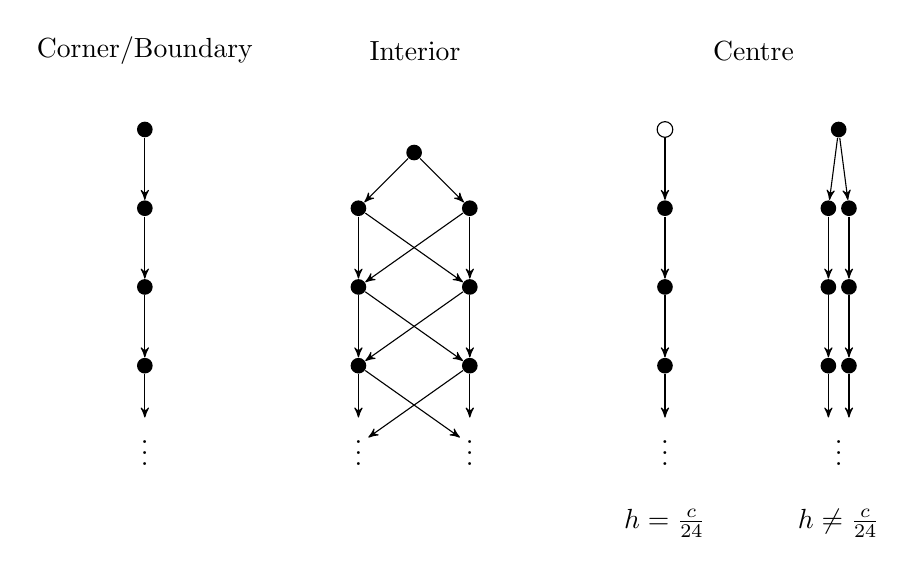
\begin{tikzpicture}[->,>=stealth', node distance=1cm]
%
  \node[sv] (b) {};
  \node[] (bdry) [above of=b] {Corner/Boundary};
  \node[sv] (ba) [below of=b] {};
  \node[sv] (bb) [below of=ba] {};
  \node[sv] (bc) [below of=bb] {};
  \node[inner sep=2pt] (bd) [below of=bc] {$\vdots$};
%
  \path[]
  (b) edge node {} (ba)
  (ba) edge node {} (bb)
  (bb) edge node {} (bc)
  (bc) edge node {} (bd);
%
  \node[sv] (ia) [right = 2.5cm of ba] {};
  \node[sv] (i) [above right of=ia] {};
  \node[] (tmp) [right = 3.2cm of b] {};
  \node[] (int) [above of=tmp] {Interior};
  \node[sv] (ib) [below of=ia] {};
  \node[sv] (ic) [below of=ib] {};
  \node[inner sep=2pt] (id) [below of =ic] {$\vdots$};
  \node[sv] (ie) [below right of =i] {};
  \node[sv] (if) [below of =ie] {};
  \node[sv] (ig) [below of =if] {};
  \node[inner sep=2pt] (ih) [below of=ig] {$\vdots$};
%
  \path[]
  (i) edge node {} (ia)
  (ia) edge node {} (ib)
  (ia) edge node {} (if)
  (ib) edge node {} (ic)
  (ib) edge node {} (ig)
  (ic) edge node {} (id)
  (ic) edge node {} (ih)
  (i) edge node {} (ie)
  (ie) edge node {} (if)
  (ie) edge node {} (ib)
  (if) edge node {} (ig)
  (if) edge node {} (ic)
  (ig) edge node {} (ih)
  (ig) edge node {} (id);	
%
  \node[osv] (c) [right = 6.4cm of b] {};
  \node[sv] (ca) [below of=c] {};
  \node[sv] (cb) [below of=ca] {};
  \node[sv] (cc) [below of=cb] {};
  \node[inner sep=2pt] (cd) [below of=cc] {$\vdots$};
  \node[] (hc) [below of=cd] {$h = \frac{c}{24}$};
%
  \path[]
  (c) edge node {} (ca)
  (ca) edge node {} (cb)
  (cb) edge node {} (cc)
  (cc) edge node {} (cd);
%
  \node[] (tmp2) [right = 0.9cm of c] {};
  \node[] [above of=tmp2]{Centre};
%
  \node[sv] (d) [right = 2cm of c] {};
  \node[] (tmp3) [below of=d] {};
  \node[sv] (da) [left = -0.1cm of tmp3] {};
  \node[sv] (db) [right = -0.1cm of tmp3] {};
  \node[sv] (dc) [below of=da] {};
  \node[sv] (dd) [below of=db] {};
  \node[sv] (de) [below of=dc] {};
  \node[sv] (df) [below of=dd] {};
  \node[inner sep=2pt] (dg) [below of=de] {$\vphantom{\vdots}$};
  \node[inner sep=2pt] (dh) [below of=df] {$\vphantom{\vdots}$};
  \node[] at (cd-|d) {$\vdots$};
  \node[] at (hc-|d) {$h \neq \frac{c}{24}$};
%
  \path[]
  (d) edge node {} (da)
  (d) edge node {} (db)
  (da) edge node {} (dc)
  (db) edge node {} (dd)
  (dc) edge node {} (de)
  (dd) edge node {} (df)
  (de) edge node {} (dg)
  (df) edge node {} (dh);
\end{tikzpicture}
\caption{The \sv{} structure of the $N=1$ Verma modules $\Ver{r,s}$ when $t \in \QQ_+$.  Each black circle corresponds to a \sv{} in the \ns{} sector and a pair of \svs{}, one bosonic and one fermionic, in the Ramond sector.  The white circle indicates a Ramond \sv{} whose multiplicity is one and the double circles indicate Ramond \svs{} of multiplicity four.  Arrows from one \sv{} (pair of \svs{}) to another indicate that the latter may be obtained from the former by acting with a suitable polynomial in the $L_n$ and $G_j$.} \label{fig:VermaStructures}
\end{figure}

Aside from the doubling of the \sv{} multiplicities in the Ramond sector, due to $G_0$, the structures of the non-centre $N=1$ Verma modules are analogous to those of the Virasoro algebra.  The new features are exhibited in the centre modules.  Despite the chain-like depiction of the \sv{} structures in \cref{fig:VermaStructures}, the centre Verma modules may be thought of as like interior modules in which the conformal weights of the \svs{} at the same horizontal level coincide (whence the multiplicity $4$ \svs{}).  However, the braided pattern of the interior modules is absent.  For $h \neq \frac{c}{24}$, each \sv{} space instead splits uniformly in two \cite{IohRepI03}, leading to the double-chain pattern of \cref{fig:VermaStructures}.

An example helps to clarify the case of the centre Verma modules.  For $(p,p') = (2,4)$, the Verma module $\Ver{1,2}$ is of centre type (the extended Kac table is given in \cref{fig:KacTables}).  As $h_{1,2} = 0 = \frac{c}{24}$, its ground state space is one-dimensional and it has two-dimensional \sv{} spaces of conformal weights $1, 4, 9, \ldots$\,.  The Verma module $\Ver{1,6} = \Ver{3,2}$ is also of centre type, with $h_{1,6} = h_{3,2} = 1$, and it has \sv{} spaces of weights $4, 9, 16, \ldots$ as well, but these are four-dimensional.  It follows that a module homomorphism from $\Ver{1,6}$ to $\Ver{1,2}$ cannot be an inclusion, a fact reinforced by consideration of their characters (see \cref{sec:CharMod} below):
\begin{equation}
\ch{\Ver{1,2}} = 1 + 2q + 4q^2 + 8q^3 + 14q^4 + \cdots, \qquad \ch{\Ver{1,6}} = 2q + 4q^2 + 8q^3 + 16q^4 + \cdots.
\end{equation}
Indeed, such a (non-zero) homomorphism maps one chain of \svs{} of $\Ver{1,6}$ onto those of $\Ver{1,2}$ and the other chain to $0$.  In other words, the submodule of $\Ver{1,2}$ generated by the \svs{} of weight $1$ is not isomorphic to a Verma module, despite the fact \cite{AubZer85} that the \uea{} of the Ramond algebra has no zero divisors.

We conclude by noting that when $h = \frac{c}{24}$, one can further relax the definition of a Ramond Verma module to allow inducing indecomposable modules over the zero mode subalgebra.  Then, one may induce the two-dimensional module spanned by the weight vectors $v$ and $G_0 v$ to obtain the module $\PreVer{c/24}$ that is called a \emph{pre-Verma module} in \cite{IohRepI03,IohStr06}.  This module is again not fixed by parity-reversal and we accordingly attach a superscript $\pm$ to match the parity of $v$.  It is, in fact, a non-split extension of the corresponding Verma module by its parity-reversed counterpart:
\begin{equation} \label{es:PreVerma}
\dses{\RVer{c/24}^{\mp}}{}{\PreVer{c/24}^{\pm}}{}{\RVer{c/24}^{\pm}}.
\end{equation}
Unlike the case of Ramond Verma modules, there are submodules of pre-Verma modules that are not generated by \svs{}.  Instead, one has to introduce \emph{\ssvs{}} which are vectors that become singular upon taking an appropriate quotient.  The structure of the pre-Verma modules was determined in \cite{IohStr06} and we indicate this structure, for $t \in \QQ_+$ hence $(r,s) = (\frac{p}{2}, \frac{p'}{2})$, in \cref{fig:PreVermaStructures}.

\begin{figure}
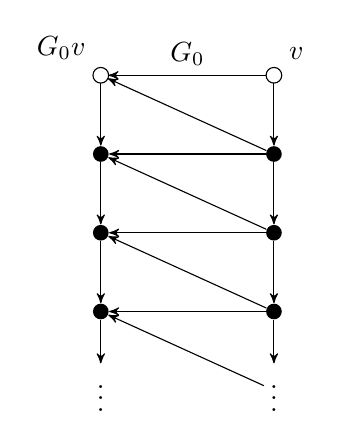
\begin{tikzpicture}[->,>=stealth', node distance=1cm]
%
  \node[osv, label=above right:{$v$}] (c) {};
  \node[osv, label=above left:{$G_0 v$}] (gc) [left = 2cm of c] {};
  \node[sv] (ca) [below of=c] {};
  \node[sv] (cb) [below of=ca] {};
  \node[sv] (cc) [below of=cb] {};
  \node[inner sep=2pt] (cd) [below of=cc] {$\vdots$};
  \node[sv] (gca) [below of=gc] {};
  \node[sv] (gcb) [below of=gca] {};
  \node[sv] (gcc) [below of=gcb] {};
  \node[inner sep=2pt] (gcd) [below of=gcc] {$\vdots$};
%
  \path[]
  (c) edge node {} (ca)
  (ca) edge node {} (cb)
  (cb) edge node {} (cc)
  (cc) edge node {} (cd)
  (gc) edge node {} (gca)
  (gca) edge node {} (gcb)
  (gcb) edge node {} (gcc)
  (gcc) edge node {} (gcd)
  (c) edge node [above] {$G_0$} (gc)
  (ca) edge node {} (gca)
  (cb) edge node {} (gcb)
  (cc) edge node {} (gcc)
  (ca) edge node {} (gc)
  (cb) edge node {} (gca)
  (cc) edge node {} (gcb)
  (cd) edge node {} (gcc);
%
\end{tikzpicture}
\caption{The \ssv{} structure of the $N=1$ pre-Verma module $\PreVer{c/24}$ for $t \in \QQ_+$.  The white circles indicate \svs{} of multiplicity $1$, the black circles on the left indicate \svs{} of multiplicity $2$, and those on the right correspond to \ssvs{} of multiplicity $2$.  Arrows between (sub)\svs{} have the same meaning as in \cref{fig:VermaStructures}.  Note that (sub)\svs{} at the same horizontal level have the same conformal weights.  The separation is intended to emphasise subsingularity and accords with \eqref{es:PreVerma}.} \label{fig:PreVermaStructures}
\end{figure}

\section{Fock spaces} \label{sec:Fock}

The $N=1$ superconformal algebras have a free field realisation as a subalgebra of the tensor product of the free boson and the free fermion vertex operator superalgebras.  In particular, the $N=1$ algebra acts on the tensor product of any Fock space over the Heisenberg algebra with either the \ns{} or Ramond fermionic Fock space.  We shall refer to such tensor products as \emph{$N=1$ Fock spaces} for brevity.

The free boson and free fermion vertex operator superalgebras are generated by fields $\func{a}{z} = \sum_{n \in \ZZ} a_n z^{-n-1}$ and $\func{b}{z} = \sum_{j \in \ZZ-1/2} b_j z^{-j-1/2}$, respectively, that satisfy
\begin{equation}
\func{a}{z} \func{a}{w} \sim \frac{1}{\brac{z-w}^2}, \qquad \func{b}{z} \func{b}{w} \sim \frac{1}{z-w}.
\end{equation}
The energy-momentum tensor and its superpartner, the generators of the $N=1$ algebra, are then given by
\begin{equation} \label{eq:DefTG}
\func{T}{z} = \frac{1}{2} \normord{\func{a}{z} \func{a}{z}} + \frac{1}{2} Q \func{\pd a}{z} + \frac{1}{2} \normord{\func{\pd b}{z} \func{b}{z}}, \qquad 
\func{G}{z} = \func{a}{z} \func{b}{z} + Q \func{\pd b}{z},
\end{equation}
where $\normord{\cdots}$ denotes normal ordering and we omit the tensor product symbols for brevity.  The resulting central charge is $c = \frac{3}{2} - 3Q^2$ which matches the $N=1$ parametrisation \eqref{eq:ParByt} if we set
\begin{equation}
\alpha = \sqrt{\frac{p \vphantom{p'}}{4p'}}, \qquad \alpha' = \sqrt{\frac{p'}{4p}}, \qquad
Q = 2 \brac{\alpha' - \alpha} = \frac{p'-p}{\sqrt{pp'}}.
\end{equation}

In the \ns{} sector, the $N=1$ Fock space $\NSFock{\lambda}$ is defined to be the tensor product of the free boson Verma module of $a_0$-eigenvalue $\lambda$ with the free fermion vacuum Verma module.  It therefore has a one-dimensional space of ground states and the conformal weight of these ground states is
\begin{subequations}
\begin{equation}
h_{\lambda} = \frac{1}{2} \lambda \brac{\lambda - Q} = \frac{4pp' \brac{\lambda - Q/2}^2 - \brac{p'-p}^2}{8pp'}.
\end{equation}
\ns{} Fock spaces inherit a choice of parity for the ground state from that of the free fermion vacuum module; as before, we indicate this choice by a superscript $\pm$.  In the Ramond sector, an $N=1$ Fock space $\RFock{\lambda}$ is the tensor product of the free boson Verma module of $a_0$-eigenvalue $\lambda$ with the free fermion Ramond Verma module.  It therefore has a two-dimensional space of ground states whose common conformal weight is
\begin{equation}
h_{\lambda} = \frac{1}{2} \lambda \brac{\lambda - Q} + \frac{1}{16} = \frac{4pp' \brac{\lambda - Q/2}^2 - \brac{p'-p}^2}{8pp'} + \frac{1}{16}.
\end{equation}
\end{subequations}
Ramond Fock spaces are preserved by the parity-reversing functor $\Pi$, even when the conformal weight of the ground states satisfies $h_{\lambda} = \frac{c}{24}$.

The contribution to the conformal weight of the ground states from the free fermion Ramond module accords perfectly with the $N=1$ parametrisation \eqref{eq:ParByt}.  Indeed, in both sectors, we have $h_{\lambda} = h_{r,s}$ when
\begin{equation} \label{eq:DefLambda}
\lambda = \lambda_{r,s} \equiv -\alpha' \brac{r-1} + \alpha \brac{s-1},
\end{equation}
with $r=s \bmod{2}$ in the \ns{} sector and $r \neq s \bmod{2}$ in the Ramond sector.  We note the following symmetries for later use:
\begin{equation} \label{eq:FFSymm}
\lambda_{r+p,s} = \lambda_{r,s} - \frac{1}{2} \sqrt{pp'}, \quad 
\lambda_{r,s+p'} = \lambda_{r,s} + \frac{1}{2} \sqrt{pp'} \qquad \Ra \qquad 
\lambda_{r+p,s+p'} = \lambda_{r,s}.
\end{equation}

We therefore define $\Fock{r,s}$ to be $\NSFock{\lambda_{r,s}}$ or $\RFock{\lambda_{r,s}}$ depending on whether $r-s$ is even or odd, respectively.  The $\Fock{r,s}$, with $r,s \in \ZZ$, exhaust the non-simple Fock spaces \cite{IohRepII03}:  A \ns{} Fock space $\NSFock{\lambda}$ is simple, unless $\lambda = \lambda_{r,s}$ with $r=s \bmod{2}$, and a Ramond Fock space $\RFock{\lambda}$ is simple, unless $\lambda = \lambda_{r,s}$ with $r \neq s \bmod{2}$.  For $t \in \QQ_+$, we depict the submodule structure of the $\Fock{r,s}$ in \cref{fig:FockStructures}.  Unlike the case of $N=1$ Verma modules, submodules of Fock spaces are generated by \ssvs{} in general.

\begin{figure}
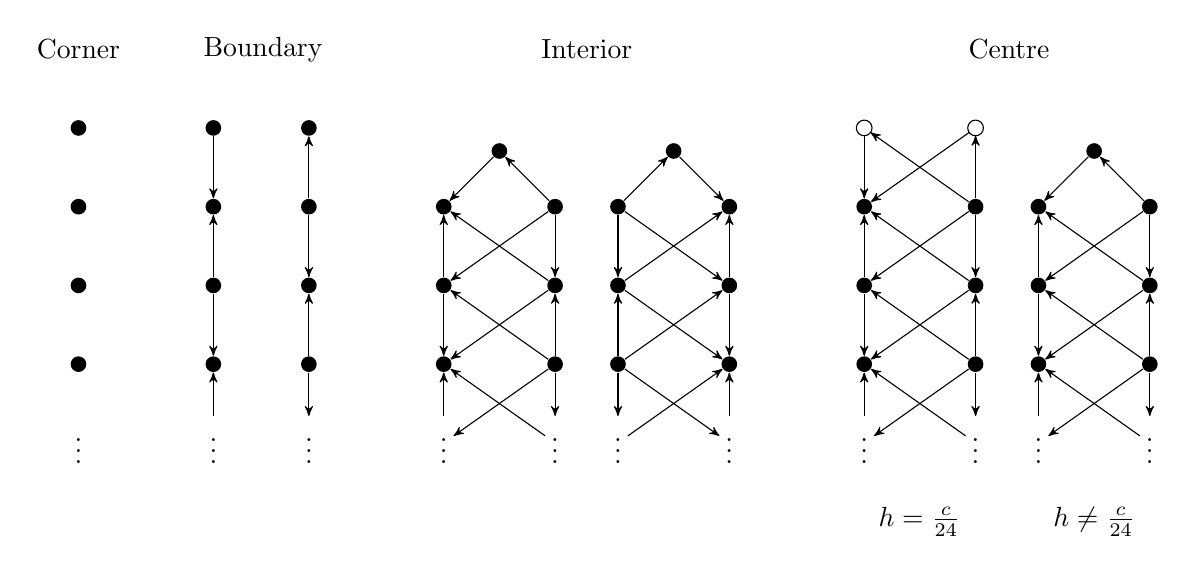
\begin{tikzpicture}[->,>=stealth', node distance=1cm]
%
  \node[sv] (a) {};
  \node[] (cor) [above of=a] {Corner};
  \node[sv] (aa) [below of=a] {};
  \node[sv] (ab) [below of=aa] {};
  \node[sv] (ac) [below of=ab] {};
  \node[inner sep=2pt] (ad) [below of=ac] {$\vdots$};
%
  \node[sv] (b) [right = 1.5cm of a] {};
  \node[sv] (ba) [below of=b] {};
  \node[sv] (bb) [below of=ba] {};
  \node[sv] (bc) [below of=bb] {};
  \node[inner sep=2pt] (bd) [below of=bc] {$\vdots$};
%
  \path[]
  (b) edge node {} (ba)
  (bb) edge node {} (ba)
  (bb) edge node {} (bc)
  (bd) edge node {} (bc);
%
  \node[] (ugh) [right = 0.4cm of b] {};
  \node[] at (ugh|-cor) {Boundary};
%
  \node[sv] (B) [right = 1cm of b] {};
  \node[sv] (Ba) [below of=B] {};
  \node[sv] (Bb) [below of=Ba] {};
  \node[sv] (Bc) [below of=Bb] {};
  \node[inner sep=2pt] (Bd) [below of=Bc] {$\vdots$};
%
  \path[]
  (Ba) edge node {} (B)
  (Ba) edge node {} (Bb)
  (Bc) edge node {} (Bb)
  (Bc) edge node {} (Bd);
%
  \node[sv] (ia) [right = 1.5cm of Ba] {};
  \node[sv] (i) [above right of=ia] {};
  \node[sv] (ib) [below of=ia] {};
  \node[sv] (ic) [below of=ib] {};
  \node[inner sep=2pt] (id) [below of =ic] {$\vdots$};
  \node[sv] (ie) [below right of =i] {};
  \node[sv] (if) [below of =ie] {};
  \node[sv] (ig) [below of =if] {};
  \node[inner sep=2pt] (ih) [below of=ig] {$\vdots$};
%
  \path[]
  (i) edge node {} (ia)
  (ib) edge node {} (ia)
  (ib) edge node {} (ic)
  (id) edge node {} (ic)
  (ie) edge node {} (i)
  (ie) edge node {} (ib)
  (ie) edge node {} (if)
  (if) edge node {} (ia)
  (if) edge node {} (ic)
  (ig) edge node {} (ib)
  (ig) edge node {} (id)
  (ig) edge node {} (if)
  (ig) edge node {} (ih)
  (ih) edge node {} (ic);
%
  \node[] (tmp) [right = 3.3cm of B] {};
  \node[] (int) [above of=tmp] {Interior};
%
  \node[sv] (Ia) [right = 2cm of ia] {};
  \node[sv] (I) [above right of=Ia] {};
  \node[sv] (Ib) [below of=Ia] {};
  \node[sv] (Ic) [below of=Ib] {};
  \node[inner sep=2pt] (Id) [below of =Ic] {$\vdots$};
  \node[sv] (Ie) [below right of =I] {};
  \node[sv] (If) [below of =Ie] {};
  \node[sv] (Ig) [below of =If] {};
  \node[inner sep=2pt] (Ih) [below of=Ig] {$\vdots$};
%
  \path[]
  (Ia) edge node {} (I)
  (Ia) edge node {} (Ib)
  (Ic) edge node {} (Ib)
  (Ic) edge node {} (Id)
  (I) edge node {} (Ie)
  (Ib) edge node {} (Ie)
  (If) edge node {} (Ie)
  (Ia) edge node {} (If)
  (Ic) edge node {} (If)
  (Ib) edge node {} (Ig)
  (Id) edge node {} (Ig)
  (If) edge node {} (Ig)
  (Ih) edge node {} (Ig)
  (Ic) edge node {} (Ih);	
%
  \node[sv] (ca) [right = 1.5cm of Ie] {};
  \node[osv] (c1) [above of=ca] {};
  \node[sv] (cb) [below of=ca] {};
  \node[sv] (cc) [below of=cb] {};
  \node[inner sep=2pt] (cd) [below of=cc] {$\vdots$};
  \node[] (ick) [right = 0.45cm of cd] {};
  \node[] (hc) [below of=ick] {$h = \frac{c}{24}$};
  \node[] (duh) [above right of=ca] {};
  \node[sv] (ce) [below right of=duh] {};
  \node[osv] (c2) [above of=ce] {};
  \node[sv] (cf) [below of=ce] {};
  \node[sv] (cg) [below of=cf] {};
  \node[inner sep=2pt] (ch) [below of=cg] {$\vdots$};
%
  \path[]
  (c1) edge node {} (ca)
  (cb) edge node {} (ca)
  (cb) edge node {} (cc)
  (cd) edge node {} (cc)
  (c2) edge node {} (ca)
  (ce) edge node {} (c1)
  (ce) edge node {} (cb)
  (ce) edge node {} (c2)
  (ce) edge node {} (cf)
  (cf) edge node {} (ca)
  (cf) edge node {} (cc)
  (cg) edge node {} (cb)
  (cg) edge node {} (cd)
  (cg) edge node {} (cf)
  (cg) edge node {} (ch)
  (ch) edge node {} (cc);
%
  \node[] (tmp2) [right = 0.2cm of c2] {};
  \node[] [above of=tmp2]{Centre};
%
  \node[sv] (Ca) [right = 2cm of ca] {};
  \node[sv] (C) [above right of=Ca] {};
  \node[sv] (Cb) [below of=Ca] {};
  \node[sv] (Cc) [below of=Cb] {};
  \node[inner sep=2pt] (Cd) [below of =Cc] {$\vdots$};
  \node[sv] (Ce) [below right of =C] {};
  \node[sv] (Cf) [below of =Ce] {};
  \node[sv] (Cg) [below of =Cf] {};
  \node[inner sep=2pt] (Ch) [below of=Cg] {$\vdots$};
  \node[] at (hc-|C) {$h \neq \frac{c}{24}$};
%
  \path[]
  (C) edge node {} (Ca)
  (Cb) edge node {} (Ca)
  (Cb) edge node {} (Cc)
  (Cd) edge node {} (Cc)
  (Ce) edge node {} (C)
  (Ce) edge node {} (Cb)
  (Ce) edge node {} (Cf)
  (Cf) edge node {} (Ca)
  (Cf) edge node {} (Cc)
  (Cg) edge node {} (Cb)
  (Cg) edge node {} (Cd)
  (Cg) edge node {} (Cf)
  (Cg) edge node {} (Ch)
  (Ch) edge node {} (Cc);
\end{tikzpicture}
\caption{The \ssv{} structure of the $N=1$ Fock spaces $\Fock{r,s}$ when $t \in \QQ_+$.  Each black circle corresponds to a \ssv{} in the \ns{} sector and a pair of \ssvs{}, one bosonic and one fermionic, in the Ramond sector.  The white circles indicate a Ramond \sv{} whose multiplicity is one.  Arrows from one \ssv{} (pair of \ssvs{}) to another have the same meaning as in \cref{fig:VermaStructures,fig:PreVermaStructures}.  The two structures for interior Fock spaces are mirror images, the repetition serving to remind us that these Fock spaces are not self-contragredient.} \label{fig:FockStructures}
\end{figure}

We remark that there are two possible structures for boundary and interior Fock spaces $\Fock{r,s}$, corresponding to the fact that these modules are not isomorphic to their contragredient duals $\Fock{Q-\lambda_{r,s}} = \Fock{-r,-s}$.  There is no ambiguity for corner and centre Fock spaces as they are self-contragredient.  For $r,s \in \ZZ_+$, the conformal weights of the \ssvs{} of the Fock space $\Fock{r,s}$ (and its contragredient $\Fock{-r,-s}$) coincide with those of the \svs{} of the Verma module $\Ver{r,s}$.  Both $\Fock{r,s}$ and $\Fock{-r,-s}$ therefore have \ssvs{} of depth $\frac{1}{2} rs$.  For $r,s \in \ZZ_+$, the depth $\frac{1}{2} rs$ \ssvs{} of $\Fock{r,s}$ are always associated to the head of the Fock space (its circle in \cref{fig:FockStructures} has all arrows pointing away from it).

This fixes the ambiguity in the structure of a boundary Fock space $\Fock{r,s}$:  One uses the symmetries \eqref{eq:FFSymm} to shift $r$ and $s$ to positive integers, thereby identifying the depth $\frac{1}{2} rs$ \ssvs{} as elements associated to the head.  Because the \ssvs{} of lesser depth are easily determined, this is sufficient to distinguish between the two possibilities in \cref{fig:FockStructures}.  For an interior Fock space $\Fock{r,s}$, this information should be supplemented by the following fact.  First, note that every second horizontal level in the interior structures of \cref{fig:FockStructures} indicates \svs{} (associated to the socle of $\Fock{r,s}$) and \ssvs{} (associated to the head).  The relevant fact is that if the depth of the \svs{} is greater than that of the \ssvs{}, at some given horizontal level, then it will also be greater at the other horizontal levels (and vice versa).  One may then check which has greater depth in a given module because one knows that the depth $\frac{1}{2} rs$ \ssvs{} is associated with the head, for $r,s \in \ZZ_+$.

It remains to discuss the centre Fock spaces.  The space of ground states is two-dimensional and the structure, when the conformal weight $h$ of the ground states is not $\frac{c}{24}$, is similar to the structure of the interior Fock spaces.  The only difference is that the \ssvs{} appearing at the same horizontal levels in \cref{fig:FockStructures} now have the same conformal weight (this never happens for interior Fock spaces).  The case where $h = \frac{c}{24}$ differs further in that the ground states do not define a simple module over the zero-mode subalgebra $\vspn \set{L_0, C, G_0}$.  Instead, the ground states decompose as a direct sum of two simple modules upon which $G_0$ acts as the zero operator.  This is easy to check as the ground states have the form $v \otimes w$ and $v \otimes b_0 w$, where $v$ is a Heisenberg \hwv{} with $a_0$-eigenvalue
\begin{equation}
\lambda_{p/2, p'/2} = -\alpha' \frac{p-2}{2} + \alpha \frac{p'-2}{2} = \alpha' - \alpha = \frac{Q}{2}
\end{equation}
and $w$ is a Ramond \hwv{} for the free fermion algebra.  Using \eqref{eq:DefTG}, we verify that
\begin{equation}
G_0 \brac{v \otimes w} = a_0 v \otimes b_0 w - \frac{Q}{2} v \otimes b_0 w = \brac{\lambda_{p/2,p'/2} - \frac{Q}{2}} v \otimes w = 0
\end{equation}
and, similarly, that $G_0 \brac{v \otimes b_0 w} = 0$.

\section{Kac modules} \label{sec:Kac}

In what follows, we will be interested in the fusion rules of certain modules $\Kac{r,s}$, indexed by $r,s \in \ZZ_+$, that we shall refer to as $N=1$ Kac modules.  Analogues of these modules over the Virasoro algebra were introduced non-constructively in \cite{PeaLog06,RasFus07,RasFus07b} in order to describe the quantum state space for a class of boundary sectors in the scaling limit of certain integrable lattice models.  Their characters were determined in many examples, but a concrete proposal for the identities of the corresponding Virasoro modules was only made recently, for corner and boundary entries $(r,s)$, as submodules of the corresponding Fock spaces \cite{RasCla11}.  More recent work \cite{MorKac15} has extended this proposal to interior entries of the extended Virasoro Kac table and has also provided a significant amount of additional evidence for its correctness.

$N=1$ Kac modules in the \ns{} sector have been recently considered from the lattice \cite{PeaLog14} and continuum \cite{CanFusI15} points of view.  The lattice analysis only studied the action of $L_0$ on a few examples, thereby obtaining a limited amount of structural information such as the presence of non-semisimple $L_0$-actions on several fusion products.  The continuum analysis built upon this by describing explicit fusion calculations that confirmed these non-semisimple actions and, moreover, detailed a series of conjectures for the structures of certain \ns{} Kac module fusion products.  

We will therefore define, the \emph{$N=1$ Kac module} $\Kac{r,s}$, with $r,s \in \ZZ_+$, to be the submodule of the Fock space $\Fock{r,s}$ that is generated by the \ssvs{} of depths strictly less than $\frac{1}{2} rs$.  This generalises the definition proposed in \cite{MorKac15} for the Virasoro algebra and \cite{CanFusI15} for the \ns{} algebra.  We note that this definition does not preclude $\Kac{r,s}$ from having \svs{} of depth $\frac{1}{2} rs$ or greater.  A selection of Kac module structures is illustrated in \cref{fig:KacStructures}.

Inspection shows that the parity-reversing functor $\Pi$ fixes each Ramond Kac module $\Kac{r,s}$ ($r+s$ odd) and maps each \ns{} Kac module ($r+s$ even) to an inequivalent counterpart.  We will therefore affix a superscript $\pm$ to indicate the ground state parity in the \ns{} sector.  Note that $\Kac{1,1}^+$ is always a \hwm{} with an even conformal weight $0$ ground state and at most $2$ composition factors.  It plays the role of the \emph{vacuum module}, meaning that it carries the structure of the universal vertex operator superalgebra (the $N=1$ algebra).

\begin{figure}
\scalebox{0.5}{
\begin{tabular}{|D{3.5cm}|D{0.5cm}|D{5.5cm}|D{0.5cm}|D{5.5cm}|D{0.5cm}|D{5.5cm}|D{0.5cm}|D{5.5cm}}
\hline
% row 1
\IKL 
%%%%%%%%%%%%%%%%%%%%%%%%%%%%%%%%% TWO CHAIN %%%%%%%%%%%%%%%%%%%%%%%%%%%%%%%%%%%
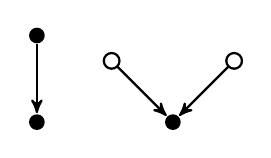
\begin{tikzpicture} 
[->,thick,-stealth', transform shape, node distance=1.1cm]
\node[sv] (1) [] {};
\node[sv] (3) [below of=1] {};
\node[sv] (5) [right=1.5cm of 3] {};
\node[osv] (4) [above left of=5] {};
\node[osv] (6) [above right of=5] {};
\path[]
   (1) edge node {} (3)
   (4) edge node {} (5)
   (6) edge node {} (5);
\end{tikzpicture}
%%%%%%%%%%%%%%%%%%%%%%%%%%%%%%%%%%%%%%%%%%%%%%%%%%%%%%%%%%%%%%%%%%%%%%%%%%%%%%
& \BKL 

\begin{tikzpicture} 
\node[sv] (1) [] {};
\end{tikzpicture}
& \IKL 
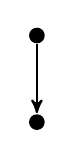
\begin{tikzpicture} 
[->,thick,-stealth', transform shape, node distance=1.1cm]
\node[sv] (1) [] {};
\node[sv] (3) [below of=1] {};
\path[]
   (1) edge node {} (3);
\end{tikzpicture}
& \BKL 

\begin{tikzpicture} 
\node[sv] (1) [] {};
\end{tikzpicture}
& \IKL 
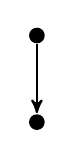
\begin{tikzpicture} 
[->,thick,-stealth', transform shape, node distance=1.1cm]
\node[sv] (1) [] {};
\node[sv] (3) [below of=1] {};
\path[]
   (1) edge node {} (3);
\end{tikzpicture}
& \BKL 

\begin{tikzpicture} 
\node[sv] (1) [] {};
\end{tikzpicture}
& \IKL 
%%%%%%%%%%%%%%%%%%%%%%%%%%%%%%%% TWO CHAIN %%%%%%%%%%%%%%%%%%%%%%%%%%%%%%%%%%%
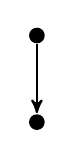
\begin{tikzpicture} 
[->,thick,-stealth', transform shape, node distance=1.1cm]
\node[sv] (1) [] {};
\node[sv] (3) [below of=1] {};
\path[]
   (1) edge node {} (3);
\end{tikzpicture}
%%%%%%%%%%%%%%%%%%%%%%%%%%%%%%%%%%%%%%%%%%%%%%%%%%%%%%%%%%%%%%%%%%%%%%%%%%%%%%
& \BKL 

\begin{tikzpicture} 
\node[sv] (1) [] {};
\end{tikzpicture}
& \IKL 
%%%%%%%%%%%%%%%%%%%%%%%%%%%%%%%%% TWO CHAIN %%%%%%%%%%%%%%%%%%%%%%%%%%%%%%%%%%%
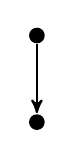
\begin{tikzpicture} 
[->,thick,-stealth', transform shape, node distance=1.1cm]
\node[sv] (1) [] {};
\node[sv] (3) [below of=1] {};
\path[]
   (1) edge node {} (3);
\end{tikzpicture}
%%%%%%%%%%%%%%%%%%%%%%%%%%%%%%%%%%%%%%%%%%%%%%%%%%%%%%%%%%%%%%%%%%%%%%%%%%%%%%
\\
\hline
% row 2
\BKL

\begin{tikzpicture}
\node[sv] (1) [] {};
\end{tikzpicture}
& 

\begin{tikzpicture}
\node[sv] (1) [] {};
\end{tikzpicture}
& \BKL 
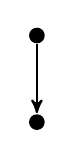
\begin{tikzpicture} 
[->,thick,-stealth', transform shape, node distance=1.1cm]
\node[sv] (1) [] {};
\node[sv] (3) [below of=1] {};
\path[]
   (1) edge node {} (3);
\end{tikzpicture}
& 

\begin{tikzpicture}
\node[sv] (1) [] {};
\end{tikzpicture}
& \BKL
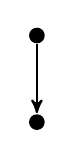
\begin{tikzpicture}
 [->,thick,-stealth', transform shape, node distance=1.1cm]
 \node[sv] (E6) [] {};
 \node[sv] (E6a) [below of=E6] {};
 \path[]
   (E6) edge node {} (E6a);
\end{tikzpicture}
& 

\begin{tikzpicture}
 \node[sv] (1) [] {};
\end{tikzpicture}
&\BKL
%%%%%%%%%%%%%%%%%%%%%%%%%%%%%%%%% TWO CHAIN %%%%%%%%%%%%%%%%%%%%%%%%%%%%%%%%%%%
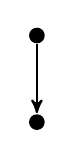
\begin{tikzpicture} 
[->,thick,-stealth', transform shape, node distance=1.1cm]
\node[sv] (1) [] {};
\node[sv] (3) [below of=1] {};
\path[]
   (1) edge node {} (3);
\end{tikzpicture}
%%%%%%%%%%%%%%%%%%%%%%%%%%%%%%%%%%%%%%%%%%%%%%%%%%%%%%%%%%%%%%%%%%%%%%%%%%%%%%
& 

\begin{tikzpicture}
 \node[sv] (1) [] {};
\end{tikzpicture}
&\BKL
%%%%%%%%%%%%%%%%%%%%%%%%%%%%%%%%% TWO CHAIN %%%%%%%%%%%%%%%%%%%%%%%%%%%%%%%%%%%
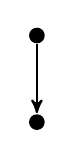
\begin{tikzpicture} 
[->,thick,-stealth', transform shape, node distance=1.1cm]
\node[sv] (1) [] {};
\node[sv] (3) [below of=1] {};
\path[]
   (1) edge node {} (3);
\end{tikzpicture}
%%%%%%%%%%%%%%%%%%%%%%%%%%%%%%%%%%%%%%%%%%%%%%%%%%%%%%%%%%%%%%%%%%%%%%%%%%%%%%
\\
\hline
% row 3
\IKL 
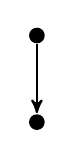
\begin{tikzpicture} 
[->,thick,-stealth', transform shape, node distance=1.1cm]
\node[sv] (1) [] {};
\node[sv] (3) [below of=1] {};
\path[]
   (1) edge node {} (3);
\end{tikzpicture}
& \BKL 
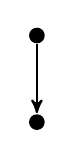
\begin{tikzpicture} 
[->,thick,-stealth', transform shape, node distance=1.1cm]
\node[sv] (1) [] {};
\node[sv] (3) [below of=1] {};
\path[]
   (1) edge node {} (3);
\end{tikzpicture}
& \IKL 
%%%%%%%%%%%%%%%%%%%%%%%%% HEXAGON %%%%%%%%%%%%%%%%%%%%%%%%%%%%
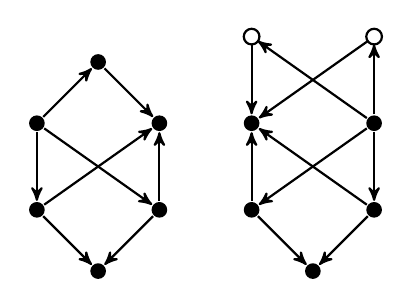
\begin{tikzpicture} 
[->,thick,-stealth', transform shape, node distance=1.1cm]
 \node[sv] (1f) [] {};
 \node[sv] (2f) [below left of=1f] {};
 \node[sv] (3f) [below right of=1f] {};
 \node[sv] (4f) [below of=2f] {};
 \node[sv] (5f) [below of=3f] {};
 \node[sv] (6f) [below left of=5f] {};
 \node[sv] (6g) [right=2.5cm of 6f] {};
 \node[sv] (5g) [above right of=6g] {};
 \node[sv] (4g) [above left of=6g] {};
 \node[sv] (3g) [above of=5g] {};
 \node[sv] (2g) [above of=4g] {};
 \node[osv] (1g) [above of=3g] {};
 \node[osv] (0g) [above of=2g] {};
 \path[]
   (2f) edge node {} (1f)
   (1f) edge node {} (3f)
   (2f) edge node {} (4f)
   (2f) edge node {} (5f)
   (4f) edge node {} (3f)
   (5f) edge node {} (3f)
   (5f) edge node {} (6f)
   (4f) edge node {} (6f)
   (0g) edge node {} (2g)
   (1g) edge node {} (2g)
   (3g) edge node {} (0g)
   (3g) edge node {} (1g)
   (3g) edge node {} (4g)
   (3g) edge node {} (5g)
   (4g) edge node {} (2g)
   (4g) edge node {} (6g)
   (5g) edge node {} (2g)
   (5g) edge node {} (6g);
\end{tikzpicture}
%%%%%%%%%%%%%%%%%%%%%%%%%%%%%%%%%%%%%%%%%%%%%%%%%%%%%%%%%%%%%%
& \BKL 
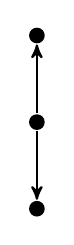
\begin{tikzpicture}
 [->,thick,-stealth', transform shape, node distance=1.1cm]
 \node[sv] (E6) [] {};
 \node[sv] (E6a) [below of=E6] {};
 \node[sv] (E6b) [below of=E6a] {};
 \path[]
   (E6a) edge node {} (E6)
   (E6a) edge node {} (E6b);
\end{tikzpicture}
& \IKL
%%%%%%%%%%%%%%%%%%%%%%%%% HEXAGON %%%%%%%%%%%%%%%%%%%%%%%%%%%%
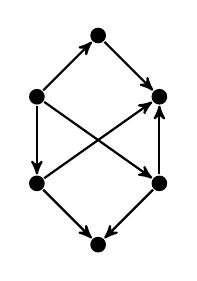
\begin{tikzpicture} 
[->,thick,-stealth', transform shape, node distance=1.1cm]
 \node[sv] (1f) [] {};
 \node[sv] (2f) [below left of=1f] {};
 \node[sv] (3f) [below right of=1f] {};
 \node[sv] (4f) [below of=2f] {};
 \node[sv] (5f) [below of=3f] {};
 \node[sv] (6f) [below left of=5f] {};
 \path[]
   (2f) edge node {} (1f)
   (1f) edge node {} (3f)
   (2f) edge node {} (4f)
   (2f) edge node {} (5f)
   (4f) edge node {} (3f)
   (5f) edge node {} (3f)
   (5f) edge node {} (6f)
   (4f) edge node {} (6f);
\end{tikzpicture}
%%%%%%%%%%%%%%%%%%%%%%%%%%%%%%%%%%%%%%%%%%%%%%%%%%%%%%%%%%%%%%
& \BKL 
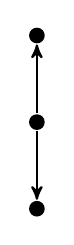
\begin{tikzpicture}
 [->,thick,-stealth', transform shape, node distance=1.1cm]
 \node[sv] (E6) [] {};
 \node[sv] (E6a) [below of=E6] {};
 \node[sv] (E6b) [below of=E6a] {};
 \path[]
   (E6a) edge node {} (E6)
   (E6a) edge node {} (E6b);
\end{tikzpicture}
&\IKL
%%%%%%%%%%%%%%%%%%%%%%%%% HEXAGON %%%%%%%%%%%%%%%%%%%%%%%%%%%%
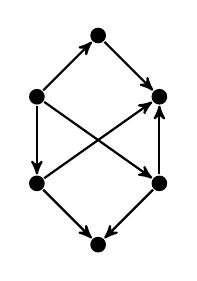
\begin{tikzpicture} 
[->,thick,-stealth', transform shape, node distance=1.1cm]
 \node[sv] (1f) [] {};
 \node[sv] (2f) [below left of=1f] {};
 \node[sv] (3f) [below right of=1f] {};
 \node[sv] (4f) [below of=2f] {};
 \node[sv] (5f) [below of=3f] {};
 \node[sv] (6f) [below left of=5f] {};
 \path[]
   (2f) edge node {} (1f)
   (1f) edge node {} (3f)
   (2f) edge node {} (4f)
   (2f) edge node {} (5f)
   (4f) edge node {} (3f)
   (5f) edge node {} (3f)
   (5f) edge node {} (6f)
   (4f) edge node {} (6f);
\end{tikzpicture}
%%%%%%%%%%%%%%%%%%%%%%%%%%%%%%%%%%%%%%%%%%%%%%%%%%%%%%%%%%%%%%
& \BKL 
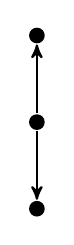
\begin{tikzpicture}
 [->,thick,-stealth', transform shape, node distance=1.1cm]
 \node[sv] (E6) [] {};
 \node[sv] (E6a) [below of=E6] {};
 \node[sv] (E6b) [below of=E6a] {};
 \path[]
   (E6a) edge node {} (E6)
   (E6a) edge node {} (E6b);
\end{tikzpicture}
&\IKL
%%%%%%%%%%%%%%%%%%%%%%%%% HEXAGON %%%%%%%%%%%%%%%%%%%%%%%%%%%%
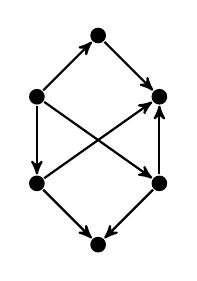
\begin{tikzpicture} 
[->,thick,-stealth', transform shape, node distance=1.1cm]
 \node[sv] (1f) [] {};
 \node[sv] (2f) [below left of=1f] {};
 \node[sv] (3f) [below right of=1f] {};
 \node[sv] (4f) [below of=2f] {};
 \node[sv] (5f) [below of=3f] {};
 \node[sv] (6f) [below left of=5f] {};
 \path[]
   (2f) edge node {} (1f)
   (1f) edge node {} (3f)
   (2f) edge node {} (4f)
   (2f) edge node {} (5f)
   (4f) edge node {} (3f)
   (5f) edge node {} (3f)
   (5f) edge node {} (6f)
   (4f) edge node {} (6f);
\end{tikzpicture}
%%%%%%%%%%%%%%%%%%%%%%%%%%%%%%%%%%%%%%%%%%%%%%%%%%%%%%%%%%%%%%
\\
\hline
% row 4
\BKL 

\begin{tikzpicture}
\node[sv] (1) [] {};
\end{tikzpicture}
& 

\begin{tikzpicture}
\node[sv] (1) [] {};
\end{tikzpicture}
& \BKL 
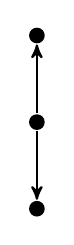
\begin{tikzpicture}
 [->,thick,-stealth', transform shape, node distance=1.1cm]
 \node[sv] (E6) [] {};
 \node[sv] (E6a) [below of=E6] {};
 \node[sv] (E6b) [below of=E6a] {};
 \path[]
   (E6a) edge node {} (E6)
   (E6a) edge node {} (E6b);
\end{tikzpicture}
& 

\begin{tikzpicture}
 [->,thick,-stealth', transform shape, node distance=1.1cm]
 \node[sv] (E6) [] {};
 \node[sv] (E6a) [below of=E6] {};
\end{tikzpicture}
& \BKL 
%%%%%%%%%%%%%%%%%%%%%%%%%%%%%%%% FOUR CHAIN %%%%%%%%%%%%%%%%%%%%%%%%%%%%%%%
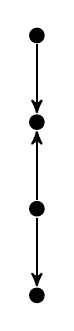
\begin{tikzpicture}
 [->,thick,-stealth', transform shape, node distance=1.1cm]
 \node[sv] (E6) [] {};
 \node[sv] (E7) [above of=E6] {};
 \node[sv] (E6a) [below of=E6] {};
 \node[sv] (E6b) [below of=E6a] {};
 \path[]
   (E7) edge node {} (E6)
   (E6a) edge node {} (E6)
   (E6a) edge node {} (E6b);
\end{tikzpicture}
%%%%%%%%%%%%%%%%%%%%%%%%%%%%%%%%%%%%%%%%%%%%%%%%%%%%%%%%%%%%%%%%%%%%%%%%%%
& 

\begin{tikzpicture}
 [->,thick,-stealth', transform shape, node distance=1.1cm]
 \node[sv] (E6) [] {};
 \node[sv] (E6a) [below of=E6] {};
\end{tikzpicture}
&\BKL
%%%%%%%%%%%%%%%%%%%%%%%%%%%%%%%% FOUR CHAIN %%%%%%%%%%%%%%%%%%%%%%%%%%%%%%%
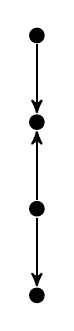
\begin{tikzpicture}
 [->,thick,-stealth', transform shape, node distance=1.1cm]
 \node[sv] (E6) [] {};
 \node[sv] (E7) [above of=E6] {};
 \node[sv] (E6a) [below of=E6] {};
 \node[sv] (E6b) [below of=E6a] {};
 \path[]
   (E7) edge node {} (E6)
   (E6a) edge node {} (E6)
   (E6a) edge node {} (E6b);
\end{tikzpicture}
%%%%%%%%%%%%%%%%%%%%%%%%%%%%%%%%%%%%%%%%%%%%%%%%%%%%%%%%%%%%%%%%%%%%%%%%%%
& 
%%%%%%%%%%%%%%%%%%%%%%%%%%%%%%% TWO CHAIN %%%%%%%%%%%%%%%%%%%%%%%%%%%%%%%%%

\begin{tikzpicture}
 [->,thick,-stealth', transform shape, node distance=1.1cm]
 \node[sv] (E6) [] {};
 \node[sv] (E6a) [below of=E6] {};
\end{tikzpicture}
%%%%%%%%%%%%%%%%%%%%%%%%%%%%%%%%%%%%%%%%%%%%%%%%%%%%%%%%%%%%%%%%%%%%%%%%%%%%
&\BKL
%%%%%%%%%%%%%%%%%%%%%%%%%%%%%%%% FOUR CHAIN %%%%%%%%%%%%%%%%%%%%%%%%%%%%%%%
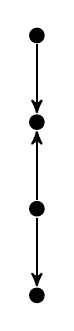
\begin{tikzpicture}
 [->,thick,-stealth', transform shape, node distance=1.1cm]
 \node[sv] (E6) [] {};
 \node[sv] (E7) [above of=E6] {};
 \node[sv] (E6a) [below of=E6] {};
 \node[sv] (E6b) [below of=E6a] {};
 \path[]
   (E7) edge node {} (E6)
   (E6a) edge node {} (E6)
   (E6a) edge node {} (E6b);
\end{tikzpicture}
%%%%%%%%%%%%%%%%%%%%%%%%%%%%%%%%%%%%%%%%%%%%%%%%%%%%%%%%%%%%%%%%%%%%%%%%%%
\\
\hline
% row 5
\IKL 
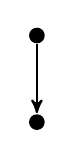
\begin{tikzpicture} 
[->,thick,-stealth', transform shape, node distance=1.1cm]
\node[sv] (1) [] {};
\node[sv] (3) [below of=1] {};
\path[]
   (1) edge node {} (3);
\end{tikzpicture}
& \BKL 
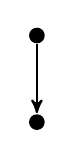
\begin{tikzpicture} 
[->,thick,-stealth', transform shape, node distance=1.1cm]
\node[sv] (1) [] {};
\node[sv] (3) [below of=1] {};
\path[]
   (1) edge node {} (3);
\end{tikzpicture}
& \IKL 
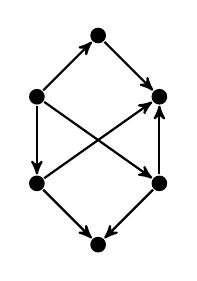
\begin{tikzpicture} 
[->,thick,-stealth', transform shape, node distance=1.1cm]
 \node[sv] (1f) [] {};
 \node[sv] (2f) [below left of=1f] {};
 \node[sv] (3f) [below right of=1f] {};
 \node[sv] (4f) [below of=2f] {};
 \node[sv] (5f) [below of=3f] {};
 \node[sv] (6f) [below left of=5f] {};
 \path[]
   (2f) edge node {} (1f)
   (1f) edge node {} (3f)
   (2f) edge node {} (4f)
   (2f) edge node {} (5f)
   (4f) edge node {} (3f)
   (5f) edge node {} (3f)
   (5f) edge node {} (6f)
   (4f) edge node {} (6f);
\end{tikzpicture}
& \BKL 
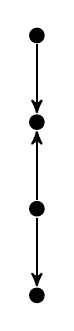
\begin{tikzpicture}
 [->,thick,-stealth', transform shape, node distance=1.1cm]
 \node[sv] (E6) [] {};
 \node[sv] (E7) [above of=E6] {};
 \node[sv] (E6a) [below of=E6] {};
 \node[sv] (E6b) [below of=E6a] {};
 \path[]
   (E7) edge node {} (E6)
   (E6a) edge node {} (E6)
   (E6a) edge node {} (E6b);
\end{tikzpicture}
& \IKL
%%%%%%%%%%%%%%%%%%%%%%%%%%%%%%%%%%% DECAGON %%%%%%%%%%%%%%%%%%%%%%%%%%%%%%%%%%%%%%%
\begin{tikzpicture} 
[->,thick,-stealth', transform shape, node distance=1.1cm]
 \node[sv] (1f) [] {};
 \node[sv] (2f) [below left of=1f] {};
 \node[sv] (3f) [below right of=1f] {};
 \node[sv] (4f) [below of=2f] {};
 \node[sv] (5f) [below of=3f] {};
 \node[sv] (6f) [below of=4f] {};
 \node[sv] (7f) [below of=5f] {};
 \node[sv] (8f) [below of =6f] {};
 \node[sv] (9f) [below of =7f] {};
 \node[sv] (10f) [below left of=9f] {};
 \node[sv] (10g) [right=2.5cm of 10f] {};
 \node[sv] (9g) [above right of=10g] {};
 \node[sv] (8g) [above left of=10g] {};
 \node[sv] (7g) [above of=9g] {};
 \node[sv] (6g) [above of=8g] {};
 \node[sv] (5g) [above of=7g] {};
 \node[sv] (4g) [above of=6g] {};
 \node[sv] (3g) [above of=5g] {};
 \node[sv] (2g) [above of=4g] {};
 \node[osv] (1g) [above of=3g] {};
 \node[osv] (0g) [above of=2g] {};
 \path[]
   (2f) edge node {} (1f)
   (1f) edge node {} (3f)
   (2f) edge node {} (4f)
   (2f) edge node {} (5f)
   (4f) edge node {} (3f)
   (5f) edge node {} (3f)
   (6f) edge node {} (4f)
   (4f) edge node {} (7f)
   (6f) edge node {} (5f)
   (5f) edge node {} (7f)
   (6f) edge node {} (8f)
   (6f) edge node {} (9f)
   (8f) edge node {} (7f)
   (9f) edge node {} (7f)
   (8f) edge node {} (10f)
   (9f) edge node {} (10f)
   (0g) edge node {} (2g)
   (1g) edge node {} (2g)
   (3g) edge node {} (0g)
   (3g) edge node {} (1g)
   (3g) edge node {} (4g)
   (3g) edge node {} (5g)
   (4g) edge node {} (2g)
   (4g) edge node {} (6g)
   (5g) edge node {} (2g)
   (5g) edge node {} (6g)
   (7g) edge node {} (4g)
   (7g) edge node {} (5g)
   (7g) edge node {} (8g)
   (7g) edge node {} (9g)
   (8g) edge node {} (6g)
   (8g) edge node {} (10g)
   (9g) edge node {} (6g)
   (9g) edge node {} (10g);
\end{tikzpicture}
%%%%%%%%%%%%%%%%%%%%%%%%%%%%%%%%%%%%%%%%%%%%%%%%%%%%%%%%%%%%%%%%%%%%%%%%%%%%%%%%%%%%%%% 
& \BKL 
%%%%%%%%%%%%%%%%%%%%%%%%%%%%%%%%%%%%%%%%%% FIVE CHAIN %%%%%%%%%%%%%%%%%%%%%%%%%%%%
\begin{tikzpicture}
 [->,thick,-stealth', transform shape, node distance=1.1cm]
 \node[sv] (E6) [] {};
 \node[sv] (E7) [above of=E6] {};
 \node[sv] (E8) [above of=E7] {};
 \node[sv] (E6a) [below of=E6] {};
 \node[sv] (E6b) [below of=E6a] {};
 \path[]
   (E7) edge node {} (E8)
   (E7) edge node {} (E6)
   (E6a) edge node {} (E6)
   (E6a) edge node {} (E6b);
\end{tikzpicture}
%%%%%%%%%%%%%%%%%%%%%%%%%%%%%%%%%%%%%%%%%%%%%%%%%%%%%%%%%%%%%%%%%%%%%%%%%%%%%%%%%
& \IKL
%%%%%%%%%%%%%%%%%%%%%%%%%%%%%%%%%%% DECAGON %%%%%%%%%%%%%%%%%%%%%%%%%%%%%%%%%%%%%%%
\begin{tikzpicture} 
[->,thick,-stealth', transform shape, node distance=1.1cm]
 \node[sv] (1f) [] {};
 \node[sv] (2f) [below left of=1f] {};
 \node[sv] (3f) [below right of=1f] {};
 \node[sv] (4f) [below of=2f] {};
 \node[sv] (5f) [below of=3f] {};
 \node[sv] (6f) [below of=4f] {};
 \node[sv] (7f) [below of=5f] {};
 \node[sv] (8f) [below of =6f] {};
 \node[sv] (9f) [below of =7f] {};
 \node[sv] (10f) [below left of=9f] {};
 \path[]
   (2f) edge node {} (1f)
   (1f) edge node {} (3f)
   (2f) edge node {} (4f)
   (2f) edge node {} (5f)
   (4f) edge node {} (3f)
   (5f) edge node {} (3f)
   (6f) edge node {} (4f)
   (4f) edge node {} (7f)
   (6f) edge node {} (5f)
   (5f) edge node {} (7f)
   (6f) edge node {} (8f)
   (6f) edge node {} (9f)
   (8f) edge node {} (7f)
   (9f) edge node {} (7f)
   (8f) edge node {} (10f)
   (9f) edge node {} (10f);
\end{tikzpicture}
%%%%%%%%%%%%%%%%%%%%%%%%%%%%%%%%%%%%%%%%%%%%%%%%%%%%%%%%%%%%%%%%%%%%%%%%%%%%%%%%%%%%%%% 
& \BKL 
%%%%%%%%%%%%%%%%%%%%%%%%%%%%%%%%%%%%%%%%%% FIVE CHAIN %%%%%%%%%%%%%%%%%%%%%%%%%%%%
\begin{tikzpicture}
 [->,thick,-stealth', transform shape, node distance=1.1cm]
 \node[sv] (E6) [] {};
 \node[sv] (E7) [above of=E6] {};
 \node[sv] (E8) [above of=E7] {};
 \node[sv] (E6a) [below of=E6] {};
 \node[sv] (E6b) [below of=E6a] {};
 \path[]
   (E7) edge node {} (E8)
   (E7) edge node {} (E6)
   (E6a) edge node {} (E6)
   (E6a) edge node {} (E6b);
\end{tikzpicture}
%%%%%%%%%%%%%%%%%%%%%%%%%%%%%%%%%%%%%%%%%%%%%%%%%%%%%%%%%%%%%%%%%%%%%%%%%%%%%%%%%
& \IKL
%%%%%%%%%%%%%%%%%%%%%%%%%%%%%%%%%%% DECAGON %%%%%%%%%%%%%%%%%%%%%%%%%%%%%%%%%%%%%%%
\begin{tikzpicture} 
[->,thick,-stealth', transform shape, node distance=1.1cm]
 \node[sv] (1f) [] {};
 \node[sv] (2f) [below left of=1f] {};
 \node[sv] (3f) [below right of=1f] {};
 \node[sv] (4f) [below of=2f] {};
 \node[sv] (5f) [below of=3f] {};
 \node[sv] (6f) [below of=4f] {};
 \node[sv] (7f) [below of=5f] {};
 \node[sv] (8f) [below of =6f] {};
 \node[sv] (9f) [below of =7f] {};
 \node[sv] (10f) [below left of=9f] {};
 \path[]
   (2f) edge node {} (1f)
   (1f) edge node {} (3f)
   (2f) edge node {} (4f)
   (2f) edge node {} (5f)
   (4f) edge node {} (3f)
   (5f) edge node {} (3f)
   (6f) edge node {} (4f)
   (4f) edge node {} (7f)
   (6f) edge node {} (5f)
   (5f) edge node {} (7f)
   (6f) edge node {} (8f)
   (6f) edge node {} (9f)
   (8f) edge node {} (7f)
   (9f) edge node {} (7f)
   (8f) edge node {} (10f)
   (9f) edge node {} (10f);
\end{tikzpicture}
%%%%%%%%%%%%%%%%%%%%%%%%%%%%%%%%%%%%%%%%%%%%%%%%%%%%%%%%%%%%%%%%%%%%%%%%%%%%%%%%%
\\
\hline
% row 6
\BKL 
\begin{tikzpicture}
\node[sv] (1) [] {};
\end{tikzpicture}
& 
\begin{tikzpicture}
\node[sv] (1) [] {};
\end{tikzpicture}
& \BKL 
\begin{tikzpicture}
 [->,thick,-stealth', transform shape, node distance=1.1cm]
 \node[sv] (E6) [] {};
 \node[sv] (E6a) [below of=E6] {};
 \node[sv] (E6b) [below of=E6a] {};
 \path[]
   (E6a) edge node {} (E6)
   (E6a) edge node {} (E6b);
\end{tikzpicture}
& 
\begin{tikzpicture} 
[->,thick,-stealth', transform shape, node distance=1.1cm]
\node[sv] (1) [] {};
\node[sv] (3) [below of=1] {};
\end{tikzpicture}
& \BKL 
%%%%%%%%%%%%%%%%%%%%%%%%%%%%%%%%%%%%%%%%%% FIVE CHAIN %%%%%%%%%%%%%%%%%%%%%%%%%%%%
\begin{tikzpicture}
 [->,thick,-stealth', transform shape, node distance=1.1cm]
 \node[sv] (E6) [] {};
 \node[sv] (E7) [above of=E6] {};
 \node[sv] (E8) [above of=E7] {};
 \node[sv] (E6a) [below of=E6] {};
 \node[sv] (E6b) [below of=E6a] {};
 \path[]
   (E7) edge node {} (E8)
   (E7) edge node {} (E6)
   (E6a) edge node {} (E6)
   (E6a) edge node {} (E6b);
\end{tikzpicture}
%%%%%%%%%%%%%%%%%%%%%%%%%%%%%%%%%%%%%%%%%%%%%%%%%%%%%%%%%%%%%%%%%%%%%%%%%%%%%%%%%
& 
\begin{tikzpicture}
 [->,thick,-stealth', transform shape, node distance=1.1cm]
 \node[sv] (E6) [] {};
 \node[sv] (E6a) [below of=E6] {};
 \node[sv] (E6b) [below of=E6a] {};
\end{tikzpicture}
&\BKL
%%%%%%%%%%%%%%%%%%%%%%%%%%%%%%%%%%%%%%%%%% SIX CHAIN %%%%%%%%%%%%%%%%%%%%%%%%%%%%
\begin{tikzpicture}
 [->,thick,-stealth', transform shape, node distance=1.1cm]
 \node[sv] (E6) [] {};
 \node[sv] (E7) [above of=E6] {};
 \node[sv] (E8) [above of=E7] {};
 \node[sv] (E9) [above of=E8] {};
 \node[sv] (E6a) [below of=E6] {};
 \node[sv] (E6b) [below of=E6a] {};
 \path[]
   (E9) edge node {} (E8)
   (E7) edge node {} (E8)
   (E7) edge node {} (E6)
   (E6a) edge node {} (E6)
   (E6a) edge node {} (E6b);
\end{tikzpicture}
%%%%%%%%%%%%%%%%%%%%%%%%%%%%%%%%%%%%%%%%%%%%%%%%%%%%%%%%%%%%%%%%%%%%%%%%%%%%%%%%%
& 
\begin{tikzpicture}
 [->,thick,-stealth', transform shape, node distance=1.1cm]
 \node[sv] (E6) [] {};
 \node[sv] (E6a) [below of=E6] {};
 \node[sv] (E6b) [below of=E6a] {};
\end{tikzpicture}
&\BKL
%%%%%%%%%%%%%%%%%%%%%%%%%%%%%%%%%%%%%%%%%% SIX CHAIN %%%%%%%%%%%%%%%%%%%%%%%%%%%%
\begin{tikzpicture}
 [->,thick,-stealth', transform shape, node distance=1.1cm]
 \node[sv] (E6) [] {};
 \node[sv] (E7) [above of=E6] {};
 \node[sv] (E8) [above of=E7] {};
 \node[sv] (E9) [above of=E8] {};
 \node[sv] (E6a) [below of=E6] {};
 \node[sv] (E6b) [below of=E6a] {};
 \path[]
   (E9) edge node {} (E8)
   (E7) edge node {} (E8)
   (E7) edge node {} (E6)
   (E6a) edge node {} (E6)
   (E6a) edge node {} (E6b);
\end{tikzpicture}
%%%%%%%%%%%%%%%%%%%%%%%%%%%%%%%%%%%%%%%%%%%%%%%%%%%%%%%%%%%%%%%%%%%%%%%%%%%%%%%%%
\end{tabular}
}
%
\caption{A depiction of the structures of the Kac modules $\Kac{r,s}$ as $(r,s)$ varies over (a part of) the extended Kac table.  The genuine Kac table, bounded by $1 \le r \le p-1$ and $1 \le s \le p'-1$, is represented by the dark grey rectangle in the upper-left corner.  Dark grey corresponds to interior and centre entries of the extended Kac table and light grey and white correspond to boundary and corner entries, respectively, as in \cref{fig:KacTables}.  When a dark grey cell contains two structures, the rightmost indicates that of a centre entry with $h = \frac{c}{24}$.  If $p=1$ or $p'=1$ (or both), then one should remove the rows or columns (or both) that contain interior labels.} \label{fig:KacStructures}
\end{figure}

\chapter{Verlinde Formula}

In order to determine the decomposition of the fusion product of two $N=1$ representations a useful tool is the Verlinde formula. A Verlinde formula gives the fusion product in terms of its characters, known as the Grothendieck ring without the action of the algebra on the fusion product space. Indecomposable modules are then considered as a sum of their composition factors. Rational theories, where the number of representations is finite, already have a well defined Verlinde formula, in the logarithmic case however an analogue will need to be found. In this chapter we will do exactly that for the $N=1$ case.

\section{Characters, modular transforms and the Verlinde formula} \label{sec:CharMod}

We report here the characters and supercharacters for the \ns{} and \ram{} Fock spaces, as well as those of the Kac modules, before turning to their behaviour under modular transformations.  The block form of the resulting S-matrix is then used to formulate a fermionic Verlinde formula from which the fusion rules of the Kac modules are easily obtained.  As characters and supercharacters are blind to the difference between a module and the direct sum of its composition factors, the fermionic Verlinde formula only allows one to deduce the multiplicities of the composition factors of a fusion product, not the module structure of the fusion product itself.  We will address questions of structure in later chapters.

\section{Modular transformations} \label{sec:Mod}

The characters and supercharacters of the Fock spaces are easily determined from those of the free boson and free fermion.  With $q = \ee^{2 \pi \ii \tau}$, as usual, we have
\begin{equation} \label{ch:Fock}
\begin{aligned}
\fch{\NSFock{\lambda}^{\pm}}{\tau} &= %q^{h_{\lambda} - c/24} \prod_{j=1}^{\infty} \frac{1+q^{j-1/2}}{1-q^j} =
\frac{q^{\brac{\lambda - Q/2}^2 / 2}}{\func{\eta}{q}} \sqrt{\frac{\fjth{3}{1;q}}{\func{\eta}{q}}}, &
%
\fch{\RFock{\lambda}}{\tau} &= %q^{h_{\lambda} - c/24} \prod_{j=1}^{\infty} \frac{1+q^j}{1-q^j} =
\frac{q^{\brac{\lambda - Q/2}^2 / 2}}{\func{\eta}{q}} \sqrt{\frac{2\,\fjth{2}{1;q}}{\func{\eta}{q}}}, \\
% Michael:  Please check, but I'm pretty sure that the "2" goes in the numerator here!
\fsch{\NSFock{\lambda}^{\pm}}{\tau} &= %q^{h_{\lambda} - c/24} \prod_{j=1}^{\infty} \frac{1-q^{j-1/2}}{1-q^j} =
\pm \frac{q^{\brac{\lambda - Q/2}^2 / 2}}{\func{\eta}{q}} \sqrt{\frac{\fjth{4}{1;q}}{\func{\eta}{q}}}, &
%
\fsch{\RFock{\lambda}}{\tau} &= 0,
\end{aligned}
\end{equation}
where we refer to \cite[App.~B]{RidSL208} for our conventions regarding Jacobi theta functions.  We note that the parity-reversing functor $\Pi$ has no effect on characters, but it negates supercharacters.  As every Ramond Fock space is fixed by $\Pi$, their supercharacters vanish identically.
%With the eta function and theta identities as follows
%\begin{equation}
%\func{\eta}{q} = q^{1/24} \prod_{j=1}^{\infty} \brac{1-q^j}, \qquad 
%\fjth{2}{z;q} = z^{1/2}q^{1/8}\prod_{j=0}^{\infty} \brac{1+zq^{j+1}} \brac{1-q^{j+1}} \brac{1+z^{-1}q^j}
%\end{equation}
%\begin{equation}
%\fjth{3}{z;q} = \prod_{j=1}^{\infty} \brac{1+zq^{j-1/2}} \brac{1-q^j} \brac{1+z^{-1}q^{j-1/2}} \qquad 
%\fjth{4}{z;q} = \prod_{j=1}^{\infty} \brac{1-zq^{j-1/2}} \brac{1-q^j} \brac{1-z^{-1}q^{j-1/2}} 
%\end{equation}

Because the \ram{} Fock space supercharacters are all trivial, there are only three modular S-transforms to compute.  These follow from the transforms of the theta functions and the evaluation of a gaussian integral:
\begin{equation} \label{eq:FockSMat}
\begin{aligned}
\fch{\NSFock{\lambda}^+}{-\frac{1}{\tau}} &= \int_{-\infty}^{\infty} \Smat{\NSFock{\lambda}^+}{\NSFock{\mu}^+} \fch{\NSFock{\mu}^+}{\tau} \: \dd \mu, \quad \Smat{\NSFock{\lambda}^+}{\NSFock{\mu}^+} = \cos \sqbrac{2 \pi (\lambda - \tfrac{Q}{2}) (\mu - \tfrac{Q}{2})},\\
%
\fch{\RFock{\lambda}}{-\frac{1}{\tau}} &= \int_{-\infty}^{\infty} \Smat{\RFock{\lambda}}{\overline{\NSFock{\mu}^+}} \fsch{\NSFock{\mu}^+}{\tau} \: \dd \mu, \quad \Smat{\RFock{\lambda}}{\overline{\NSFock{\mu}^+}} = \sqrt{2} \cos \sqbrac{2 \pi (\lambda - \tfrac{Q}{2}) (\mu - \tfrac{Q}{2})},\\
%
\fsch{\NSFock{\lambda}^+}{-\frac{1}{\tau}} &= \int_{-\infty}^{\infty} \Smat{\overline{\NSFock{\lambda}^+}}{\RFock{\mu}} \fch{\RFock{\mu}}{\tau} \: \dd \mu, \quad \Smat{\overline{\NSFock{\lambda}^+}}{\RFock{\mu}} = \frac{1}{\sqrt{2}} \cos \sqbrac{2 \pi (\lambda - \tfrac{Q}{2}) (\mu - \tfrac{Q}{2})}.
\end{aligned}
\end{equation}
%
Here, we have indicated S-transforms involving a supercharacter, instead of a character, by a bar.  We have also assumed that the parity of each \ns{} Fock space is positive for simplicity.  S-matrix entries involving negative parities follow immediately from $\ch{\NSFock{\lambda}^-} = \ch{\NSFock{\lambda}^+}$ and $\sch{\NSFock{\lambda}^-} = -\sch{\NSFock{\lambda}^+}$.  Finally, we have followed \cite{CanFusI15} in extending the natural integration range from $[\frac{Q}{2}, \infty)$ to $(-\infty,\infty)$.  This convenience is allowed because $\Fock{\lambda}^{\pm}$ and its contragredient dual $\Fock{Q-\lambda}^{\pm}$ have the same (super)character.

With respect to the block-ordering $\set{\ch{\NSFock{}}, \ch{\RFock{}}, \sch{\NSFock{}}}$ of characters and supercharacters, the Fock space S-matrix may be summarised as
\begin{equation}
\begin{pmatrix}
\Smat{\NSFock{\lambda}}{\NSFock{\mu}} & 0 & 0 \\
0 & 0 & \Smat{\overline{\NSFock{\lambda}}}{\RFock{\mu}} \\
0 &\Smat{\RFock{\lambda}}{\overline{\NSFock{\mu}}} & 0
\end{pmatrix}
.
\end{equation}
We note that this S-matrix is not symmetric in this basis, but it is easily checked to be unitary and to square to the conjugation permutation.

The Fock spaces constitute a set of \emph{standard modules} \cite{CreLog13,RidVer14} for the $N=1$ algebra.  This means, among other things, that their characters form a (topological) basis for the space spanned by the characters of all the $N=1$ modules (in the module category of interest).  In particular, the Kac module characters must be expressible in terms of Fock space characters.  Recall that $\Kac{r,s}$ is a submodule of $\Fock{r,s}$, by definition.  Inspection shows that the quotient $\Fock{r,s} / \Kac{r,s}$ is not isomorphic to another Fock space or Kac module, in general, but that the character of the quotient matches that of a Fock space.  More precisely, we have the identity
\begin{equation} \label{eq:KacChar}
\ch{\Kac{r,s}} = \ch{\Fock{r,s}} - \ch{\Fock{-r,s}} = \ch{\Fock{r,s}} - \ch{\Fock{r,-s}}.
\end{equation}
The analogous identity for supercharacters is a little more complicated.  Since $h_{-r,s} = h_{r,s} + \frac{1}{2} rs$, it follows that $\Fock{r,s}$ and (the submodule whose character matches that of) $\Fock{-r,s}$ have opposite parity in the \ns{} sector, if $r$ and $s$ are both odd, and the same parity if $r$ and $s$ are both even.  In the Ramond sector, the supercharacters all vanish, hence
\begin{equation} \label{eq:KacSChar}
\begin{aligned}
\sch{\Kac{r,s}^{\pm}} &= \sch{\Fock{r,s}^{\pm}} - (-1)^r \sch{\Fock{-r,s}^{\pm}} & &\text{(\(r+s\) even),} \\
\sch{\Kac{r,s}} &= 0 & &\text{(\(r+s\) odd).}
\end{aligned}
\end{equation}

It is worth noting at this point that \eqref{eq:KacChar} and \eqref{eq:KacSChar} allow one to formally extend the Kac characters and supercharacters from $r,s \in \ZZ_+$ to all $r,s \in \ZZ$.  Upon doing this, one arrives at the relations
\begin{equation} \label{eq:ChSchRels}
\begin{gathered}
\ch{\Kac{-r,s}} = -\ch{\Kac{r,s}} = \ch{\Kac{r,-s}}, \quad \ch{\Kac{r,0}} = \ch{\Kac{0,s}} = 0, \quad \ch{\Kac{-r,-s}} = \ch{\Kac{r,s}}, \\
\sch{\Kac{r,s}^{\pm}} = -(-1)^r \sch{\Kac{-r,s}^{\pm}} = -(-1)^s \sch{\Kac{r,-s}^{\pm}} = \sch{\Kac{-r,-s}^{\pm}}.
\end{gathered}
\end{equation}
These relations will be important for interpreting the Verlinde formula calculations that follow.

By combining \eqref{eq:FockSMat} with \eqref{eq:KacChar} and \eqref{eq:KacSChar}, we obtain the S-matrix entries for the Kac module characters and supercharacters as differences of Fock space S-matrix entries:
\begin{equation}
\begin{aligned}
\Smat{\Kac{r,s}^+}{\NSFock{\mu}^+} &= 2 \sin \sqbrac{2 \pi \alpha' r (\mu - \tfrac{Q}{2})} \sin \sqbrac{2 \pi \alpha s (\mu - \tfrac{Q}{2})} \mspace{50mu} \text{(\(r+s\) even),} \\
\Smat{\Kac{r,s}}{\overline{\NSFock{\mu}^+}} &= 2 \sqrt{2} \sin \sqbrac{2 \pi \alpha' r (\mu - \tfrac{Q}{2})} \sin \sqbrac{2 \pi \alpha s (\mu - \tfrac{Q}{2})} \mspace{30mu} \text{(\(r+s\) odd),} \\
\Smat{\overline{\Kac{r,s}^+}}{\RFock{\mu}} &=
\begin{cases}
\sqrt{2} \cos \sqbrac{2 \pi \alpha' r (\mu - \tfrac{Q}{2})} \cos \sqbrac{2 \pi \alpha s (\mu - \tfrac{Q}{2})} & \text{(\(r\), \(s\) odd),} \\[1ex]
\sqrt{2} \sin \sqbrac{2 \pi \alpha' r (\mu - \tfrac{Q}{2})} \sin \sqbrac{2 \pi \alpha s (\mu - \tfrac{Q}{2})} & \text{(\(r\), \(s\) even).}
\end{cases}
\end{aligned}
\end{equation}
Again, we have assumed positive parity ground states in the \ns{} sector for simplicity.  We remark that S-matrix entries of the form $\Smat{\Kac{r,s}}{\Kac{r',s'}}$ are not defined in this setup.

\section{Verlinde products} \label{sec:VerProd}

In this section we give the Verlinde formula for subring of Kac characters contained within the Grothendieck ring of  \ns{} characters before considering the entire $N=1$ algebra. This case is simpler than the complete case and will serve as a template for the following section, where \ram{} characters will be introduced. We calculate the character product of the generators with an arbitrary module using this formula as well as giving the general rules for a character product in this subring. 

Assuming that the fusion product ``$\fuse$'' descends to a well defined product ``$\Grfuse$'' on the Grothendieck ring of characters, we may decompose a character product into a linear combination of Fock space characters:
\begin{equation}
\ch{\mathcal{M} \fuse \mathcal{N}} = \ch{\mathcal{M}} \Grfuse \ch{\mathcal{N}} = \int_{-\infty}^{\infty} \fuscoeff{\mathcal{M}}{\mathcal{N}}{\Fock{\nu}} \ch{\Fock{\nu}} \: \dd \nu.
\end{equation}
Here, $\mathcal{M}$ and $\mathcal{N}$ are \ns{} modules and we recall that the Fock space characters are the preferred (topological) basis for the space of all \ns{} characters.  The multiplicities $\fuscoeff{\mathcal{M}}{\mathcal{N}}{\Fock{\nu}}$ are the Verlinde coefficients and are computed, in terms of the S-transformation kernel, by the Verlinde formula:
\begin{equation}
\fuscoeff{\mathcal{M}}{\mathcal{N}}{\Fock{\nu}} = \int_{-\infty}^{\infty} \frac{\Smat{\mathcal{M}}{\Fock{\rho}} \Smat{\mathcal{N}}{\Fock{\rho}} \Smat{\Fock{\nu}}{\Fock{\rho}}^*}{\Smat{\Kac{1,1}}{\Fock{\rho}}} \: \dd \rho.
\end{equation}
Here, $\Kac{1,1}$ plays the role of the vacuum module.  Note that this Kac module is generated by a \hws{} of conformal weight $0$ that is annihilated by both $L_{-1}$ and $G_{-1/2}$.

It is now straight-forward to compute the character of fusion products.  The unitarity of the S-transformation implies that the vacuum module $\Kac{1,1}$ is the unit of the character product:  
\begin{equation}
\ch{\Kac{1,1} \fuse \mathcal{N}} = \ch{\Kac{1,1}} \Grfuse \ch{\mathcal{N}} = \ch{\mathcal{N}}.
\end{equation}
A somewhat less trivial example involves the fusion of $\Kac{3,1}$ with an arbitrary Fock space:
\begin{subequations}
\begin{align}
\fuscoeff{\Kac{3,1}}{\Fock{\mu}}{\Fock{\nu}} &= \int_{-\infty}^{\infty} \frac{\Smat{\Kac{3,1}}{\Fock{\rho}} \Smat{\Fock{\mu}}{\Fock{\rho}} \Smat{\Fock{\nu}}{\Fock{\rho}}^*}{\Smat{\Kac{1,1}}{\Fock{\rho}}} \: \dd \rho \notag \\
&= \int_{-\infty}^{\infty} \frac{\sin \sqbrac{6 \pi \alpha' \rho}}{\sin \sqbrac{2 \pi \alpha' \rho}} \cos \sqbrac{2 \pi \brac{\mu - Q/2} \rho} \cos \sqbrac{2 \pi \brac{\nu - Q/2} \rho} \: \dd \rho \notag \\
&= \frac{1}{2} \int_{-\infty}^{\infty} \brac{1 + 2 \cos \sqbrac{4 \pi \alpha' \rho}} \brac{\cos \sqbrac{2 \pi \brac{\mu - \nu} \rho} + \cos \sqbrac{2 \pi \brac{\mu + \nu - Q} \rho}} \: \dd \rho \notag \\
&= \func{\delta}{\nu = \mu - 2 \alpha'} + \func{\delta}{\nu = \mu} + \func{\delta}{\nu = \mu + 2 \alpha'} \notag \\
\Ra \qquad \ch{\Kac{3,1}} \Grfuse \ch{\Fock{\mu}} &= \ch{\Fock{\mu - 2 \alpha'}} + \ch{\Fock{\mu}} + \ch{\Fock{\mu + 2 \alpha'}}.
\intertext{Similar computations result in}
\ch{\Kac{1,3}} \Grfuse \ch{\Fock{\mu}} &= \ch{\Fock{\mu - 2 \alpha}} + \ch{\Fock{\mu}} + \ch{\Fock{\mu + 2 \alpha}}, \\
\ch{\Kac{2,2}} \Grfuse \ch{\Fock{\mu}} &= \ch{\Fock{\mu - \alpha' - \alpha}} + \ch{\Fock{\mu - \alpha' + \alpha}} + \ch{\Fock{\mu + \alpha' - \alpha}} + \ch{\Fock{\mu + \alpha' + \alpha}}.
\end{align}
\end{subequations}
Using \cref{ch:Kac}, we obtain the corresponding products with arbitrary Kac modules:
\begin{subequations}
\begin{align}
\ch{\Kac{3,1}} \Grfuse \ch{\Kac{r,s}} &= \ch{\Kac{r-2,s}} + \ch{\Kac{r,s}} + \ch{\Kac{r+2,s}}, \label{GrFR:K31xK} \\
\ch{\Kac{1,3}} \Grfuse \ch{\Kac{r,s}} &= \ch{\Kac{r,s-2}} + \ch{\Kac{r,s}} + \ch{\Kac{r,s+2}}, \label{GrFR:K13xK} \\
\ch{\Kac{2,2}} \Grfuse \ch{\Kac{r,s}} &= \ch{\Kac{r-1,s-1}} + \ch{\Kac{r-1,s+1}} + \ch{\Kac{r+1,s-1}} + \ch{\Kac{r+1,s+1}}. \label{GrFR:K22xK}
\end{align}
\end{subequations}
Here, we must employ \eqref{eq:KacCharSymm} if the labels on the Kac modules of the \rhs{} are not positive integers.

It follows from these character products that the Kac characters span a unital subring of the Grothendieck ring of \ns{} characters and that this subring is generated by $\ch{\Kac{3,1}}$, $\ch{\Kac{2,2}}$ and $\ch{\Kac{1,3}}$.\footnote{There is a simple exception when $c=\frac{3}{2}$ ($p=p'=1$) because then $\ch{\Kac{3,1}} = \ch{\Kac{1,3}}$ and $\ch{\Kac{2,2}} = \ch{\Kac{1,1}} + \ch{\Kac{1,3}}$.}  Associativity then leads to an explicit general formula for Kac character products:
\begin{equation} \label{GrFR:KxK}
\ch{\Kac{r,s}} \Grfuse \ch{\Kac{r',s'}} = \sideset{}{'} \sum_{r'' = \abs{r-r'}+1}^{r+r'-1} \ \sideset{}{'} \sum_{s'' = \abs{s-s'}+1}^{s+s'-1} \ch{\Kac{r'',s''}}.
\end{equation}
Here, the primed sums indicate that the summation variable increases in steps of two.  We mention, for later purposes, the following special case:
\begin{equation} \label{GrFR:Kr1xK1s}
\ch{\Kac{r,1}} \Grfuse \ch{\Kac{1,s}} = \ch{\Kac{r,s}}.
\end{equation}

\section{A fermionic Verlinde formula} \label{sec:FermVer}

The standard Verlinde formula fails to give a meaningful result when applied to the $N=1$ algebra. This is due to the fact that the $S$-matrix now contains many zeroes, that will lead to an infinite denominator in some cases. It is necessary to then consider this new $S$-matrix and construct a Verlinde formula that will give meaningful results.

In this section, we provide a derivation of the fermionic Verlinde formula \eqref{eq:Verlinde}.  This extends the results of \cite{EhoFus94} and rests on one main assumption, that the standard module formalism of \cite{CreLog13,RidVer14} applies to the bosonic orbifold of the $N=1$ algebra.  As the application at hand only involves \ns{} modules whose supercharacters are non-vanishing and Ramond modules whose supercharacters vanish, we will incorporate these facts into the derivation and thereby simplify it.  A more general derivation will appear in \cite{MelVer15}.

We note that each $N=1$ vertex operator superalgebra admits an order $2$ automorphism that fixes the even (bosonic) elements and negates the odd (fermionic) ones.  The corresponding orbifold is the vertex operator algebra spanned by the bosonic elements.  The assumption that this bosonic orbifold admits a collection of standard modules implies that the Grothendieck fusion rules of the orbifold may be computed using the standard Verlinde formula.  We compute these rules in terms of $N=1$ data, thereby reconstructing a Verlinde formula for the $N=1$ algebras.

The derivation is conveniently cast in the language of induction and restriction.  To start, we note that the vacuum module $\Kac{1,1}^+$ of the $N=1$ algebra restricts to the direct sum of its bosonic states, which form the vacuum module $\Mod{I}^+$ of the bosonic orbifold, and its fermionic states, which form a module $\Mod{J}^-$ over the orbifold algebra.  Conversely, inducing either orbifold module to an $N=1$ module recovers the $N=1$ vacuum module.  Thus,
\begin{equation} \label{eq:ResVacMod}
\Res{\Kac{1,1}^+} = \Mod{I}^+ \oplus \Mod{J}^-, \qquad \Ind{\Mod{I}^+} = \Ind{\Mod{J}^-} = \Kac{1,1}^+.
\end{equation}
It is sometimes convenient to remember the parities inherited in this fashion by orbifold modules, even though the natural $\ZZ_2$-grading on the bosonic orbifold algebra is trivial (parity is meaningless for bosonic algebras).  For example, such considerations show that $\Mod{J}^-$ is a simple current of order two:
\begin{equation}
\Ind{\brac{\Mod{J}^- \fuse \Mod{J}^-}} = \Ind{\Mod{J}^-} \fuse \Ind{\Mod{J}^-} = \Kac{1,1}^+ \fuse \Kac{1,1}^+ = \Kac{1,1}^+ \qquad \Ra \qquad \Mod{J}^- \fuse \Mod{J}^- = \Mod{I}^+.
\end{equation}
Here, we have used \cite[Eq.~(3.3)]{RidVer14} to compute the induction of the fusion product on the \lhs{} and noted that the only alternative conclusion would be that $\Mod{J}^- \fuse \Mod{J}^- = \Mod{J}^-$ (which violates parity).  It follows that the $N=1$ algebra is the simple current extension, by $\Mod{J}^-$, of the orbifold algebra.

This restriction and induction generalises to $N=1$ modules (we consider only Fock spaces and Kac modules for simplicity) and the corresponding orbifold modules as follows.  In the \ns{} sector, we may take restriction and induction to act as
\begin{equation} \label{eq:IndResNS}
\Res{\Mod{M}^{\pm}} = \Orb{}^+ \oplus (\Mod{J}^- \times \Orb{}^+), \qquad \Ind{\Orb{}^+} = \Mod{M}^+, \quad \Ind{(\Mod{J}^- \times \Orb{}^+)} = \Mod{M}^-,
\end{equation}
where we take $\Orb{}^+$ to consist of the bosonic states of $\Mod{M}^{\pm}$ (regardless of the latter's parity).  This means that the ground states of $\Mod{M}^+$ may be identified with those of $\Orb{}^+$, while the ground states of $\Mod{M}^-$ should be identified with those of $\Mod{J}^- \times \Orb{}^+$.  In the Ramond sector, things are more straightforward because there is no need to indicate the parity.  The restriction and induction functors act as
\begin{equation} \label{eq:IndResR}
\Res{\Mod{M}} = \Orb{} \oplus \Orb{}, \qquad \Ind{\Orb{}} = \Mod{M},
\end{equation}
because $\Orb{} \fuse \Mod{J}^- = \Orb{}$.  From here on, we will omit parity labels on all orbifold modules.

Define the orbifold modules $\NSOrb{\lambda}$, $\Mod{J} \fuse \NSOrb{\lambda}$ and $\ROrb{\lambda}$, for $\lambda \in \RR$, to consist of the bosonic states of $\NSFock{\lambda}^+$, $\NSFock{\lambda}^-$ and $\RFock{\lambda}$, respectively, as in \eqref{eq:IndResNS} and \eqref{eq:IndResR}.  We will assume that these define a set of standard modules for the orbifold vertex operator algebra.  In particular, their characters are linearly independent.  The correspondences $\NSOrb{\lambda} \leftrightarrow \NSFock{\lambda}^+$, $\Mod{J} \fuse \NSOrb{\lambda} \leftrightarrow \NSFock{\lambda}^-$ and $\ROrb{\lambda} \leftrightarrow \RFock{\lambda}$ are each one-to-one.  However, the analogous correspondence between characters is only two-to-one in the \ns{} sector because characters do not distinguish $\NSFock{\lambda}^+$ from $\NSFock{\lambda}^-$.  The correspondence for \ns{} supercharacters is likewise two-to-one as $\sch{\NSFock{\lambda}^+} = -\sch{\NSFock{\lambda}^-}$, though that of the Ramond characters remains one-to-one.  It follows that in the \ns{} sector, integrating over all the standard orbifold characters, $\ch{\NSOrb{\lambda}}$ and $\ch{\Mod{J} \fuse \NSOrb{\lambda}}$, is equivalent to integrating over all the standard $N=1$ characters, $\ch{\NSFock{\lambda}}$, \emph{twice}, and the same is true for supercharacters.  However, integrating over the $\ch{\ROrb{\lambda}}$ is the same as integrating over all the $\ch{\RFock{\lambda}}$.

With this preparation, we can now relate the S-matrix entries, in the basis of standard characters, of the $N=1$ theory to those of its bosonic orbifold.  For this, it is convenient to introduce the \emph{monodromy charge} $Q(\Orb{})$ of an orbifold module $\Orb{}$ (with respect to the simple current $\Mod{J}$) \cite{SchExt89}:
\begin{equation}
Q(\Orb{}) = h(\Orb{}) + h(\Mod{J}) - h(\Mod{J} \fuse \Orb{}) =
\begin{cases}
0 & \text{if \(\Ind{\Orb{}}\) is \ns{},} \\
\frac{1}{2} & \text{if \(\Ind{\Orb{}}\) is Ramond.}
\end{cases}
\end{equation}
Here, $h(\Orb{})$ denotes the conformal weight of the ground states of $\Orb{}$ so, in particular, $h(\Mod{J}) = \frac{3}{2}$.  The point is that the monodromy charge governs how the simple current acts on the S-matrix entries \cite{SchSimp90}:
\begin{equation} \label{eq:SConSMat}
\OrbSmat{\Mod{J} \fuse \Orb{}}{\Orb{}'} = \ee^{2 \pi \ii Q(\Orb{}')} \OrbSmat{\Orb{}}{\Orb{}'} =
\begin{cases}
+\OrbSmat{\Orb{}}{\Orb{}'} & \text{if \(\Ind{\Orb{}'}\) is \ns{},} \\
-\OrbSmat{\Orb{}}{\Orb{}'} & \text{if \(\Ind{\Orb{}'}\) is Ramond.}
\end{cases}
\end{equation}
Here, $\Orb{}$ and $\Orb{}'$ are standard orbifold modules ($\NSOrb{\lambda}$, $\Mod{J} \fuse \NSOrb{\lambda}$, $\ROrb{\lambda}$) and we denote the S-matrix of the bosonic orbifold by $\OrbmodS$ to distinguish it from $\modS$, the S-matrix of the $N=1$ algebra.  The analogous relation for $\OrbSmat{\Orb{}}{\Mod{J} \times \Orb{}'}$ now follows from the symmetry of the orbifold S-matrix in the standard basis \cite{RidVer14}.

From $\Res{\NSFock{\lambda}^+} = \NSOrb{\lambda} \oplus (\Mod{J} \times \NSOrb{\lambda})$ (we choose positive parities as in \cref{sec:Mod}), we deduce that
\begin{equation}
\Sch{\NSFock{\lambda}^+}
= \int \brac{\OrbSmat{\NSOrb{\lambda}}{\Orb{}} + \OrbSmat{\Mod{J} \fuse \NSOrb{\lambda}}{\Orb{}}} \ch{\Orb{}} \: \dd \Orb{}
= \int_{\Ind{\Orb{}} \in \text{NS}} 2 \, \OrbSmat{\NSOrb{\lambda}}{\Orb{}} \ch{\Orb{}} \: \dd \Orb{},
\end{equation}
where the first integral is over all the standard orbifold modules and the second is over the $\NSOrb{\mu}$ and $\Mod{J} \fuse \NSOrb{\mu}$ that induce to \ns{} $N=1$ modules.  It follows that
\begin{align}
\Sch{\NSFock{\lambda}^+}
&= \int_{-\infty}^{\infty} 2 \, \Bigl( \OrbSmat{\NSOrb{\lambda}}{\NSOrb{\mu}} \ch{\NSOrb{\mu}} + \OrbSmat{\NSOrb{\lambda}}{\Mod{J} \fuse \NSOrb{\mu}} \ch{\Mod{J} \fuse \NSOrb{\mu}} \Bigr) \: \dd \mu \notag \\
&= \int_{-\infty}^{\infty} 2 \, \OrbSmat{\NSOrb{\lambda}}{\NSOrb{\mu}} \Bigl( \ch{\NSOrb{\mu}} + \ch{\Mod{J} \fuse \NSOrb{\mu}} \Bigr) \: \dd \mu \notag \\
&= \int_{-\infty}^{\infty} 2 \, \OrbSmat{\NSOrb{\lambda}}{\NSOrb{\mu}} \ch{\NSFock{\mu}^+} \: \dd \mu,
\end{align}
where we have used \eqref{eq:SConSMat} to simplify the S-transform.  We conclude that
\begin{subequations} \label{eq:SFerm=SBos}
\begin{align}
\Smat{\NSFock{\lambda}^+}{\NSFock{\mu}^+} &= 2 \, \OrbSmat{\NSOrb{\lambda}}{\NSOrb{\mu}}.
\intertext{Similar calculations result in}
\Smat{\RFock{\lambda}}{\overline{\NSFock{\mu}^+}} &= 2 \, \OrbSmat{\ROrb{\lambda}}{\NSOrb{\mu}}, \\
\Smat{\overline{\NSFock{\lambda}^+}}{\RFock{\mu}} &= \OrbSmat{\NSOrb{\lambda}}{\ROrb{\mu}},
\end{align}
\end{subequations}
recalling that the bar indicates the supercharacter.  The other S-matrix entries vanish.

There are almost identical relations holding for the S-matrix entries involving the Kac modules.  As restricting an $N=1$ module to its bosonic or fermionic orbifold submodule defines an exact functor, the analogues of the Kac modules in the orbifold theory have characters satisfying similar identities to \eqref{eq:KacChar}.  The analogues of \eqref{eq:SFerm=SBos} then follow readily.  In particular, the vacuum S-matrix entries satisfy
\begin{equation} \label{eq:SFerm=SBosVac}
\Smat{\Kac{1,1}^+}{\NSFock{\mu}^+} = 2 \, \OrbSmat{\Mod{I}}{\NSOrb{\mu}}, \qquad
\Smat{\overline{\Kac{1,1}^+}}{\RFock{\mu}} = \OrbSmat{\Mod{I}}{\ROrb{\mu}},
\end{equation}
where we recall that $\Mod{I}$ denotes the vacuum module of the orbifold algebra.



\section{Grothendieck fusion products} \label{sec:VerProd}

We turn now to the Verlinde product of two orbifold modules, $\Mod{M}$ and $\Mod{N}$, and their $N=1$ inductions:
\begin{align}
\ch{\Ind{\Mod{M}}} \Grfuse \ch{\Ind{\Mod{N}}} &= \ch{\Ind{\Mod{M}} \fuse \Ind{\Mod{N}}} = \ch{\Ind{(\Mod{M} \fuse \Mod{N})}} = \brac{\ch{\Mod{I}} + \ch{\Mod{J}}} \Grfuse \ch{\Mod{M} \fuse \Mod{N}} \notag \\
&= \brac{\ch{\Mod{I}} + \ch{\Mod{J}}} \Grfuse \int \orbfuscoeff{\Mod{M}}{\Mod{N}}{\Orb{}} \ch{\Orb{}} \: \dd \Orb{} = \int \orbfuscoeff{\Mod{M}}{\Mod{N}}{\Orb{}} \ch{\Ind{\Orb{}}} \: \dd \Orb{},
\end{align}
where the integration is over all the standard orbifold modules and the $\orbfuscoeff{\Mod{M}}{\Mod{N}}{\Orb{}}$ denote the Verlinde coefficients of the orbifold algebra.  As $\ch{\Ind{\NSOrb{\nu}}} = \ch{\NSFock{\nu}^+} = \ch{\NSFock{\nu}^-} = \ch{\Ind{(\Mod{J} \fuse \NSOrb{\nu})}}$, we arrive at
\begin{equation}
\ch{\Ind{\Mod{M}}} \Grfuse \ch{\Ind{\Mod{N}}} = \int_{-\infty}^{\infty} \brac{\orbfuscoeff{\Mod{M}}{\Mod{N}}{\NSOrb{\nu}} + \orbfuscoeff{\Mod{M}}{\Mod{N}}{\Mod{J} \fuse \NSOrb{\nu}}} \ch{\NSFock{\nu}^+} \: \dd \nu + \int_{-\infty}^{\infty} \orbfuscoeff{\Mod{M}}{\Mod{N}}{\ROrb{\nu}} \ch{\RFock{\nu}} \: \dd \nu,
\end{equation}
hence the $N=1$ Verlinde coefficients satisfy
\begin{subequations} \label{eq:VerCoeff}
\begin{equation} \label{eq:VerCoeffChar}
\fuscoeff{\Ind{\Mod{M}}}{\Ind{\Mod{N}}}{\NSFock{\nu}^+} = \orbfuscoeff{\Mod{M}}{\Mod{N}}{\NSOrb{\nu}} + \orbfuscoeff{\Mod{M}}{\Mod{N}}{\Mod{J} \fuse \NSOrb{\nu}}, \qquad 
\fuscoeff{\Ind{\Mod{M}}}{\Ind{\Mod{N}}}{\RFock{\nu}} = \orbfuscoeff{\Mod{M}}{\Mod{N}}{\ROrb{\nu}}.
\end{equation}
Repeating this analysis for supercharacters gives instead
\begin{equation} \label{eq:VerCoeffSChar}
\fuscoeff{\overline{\Ind{\Mod{M}}}}{\overline{\Ind{\Mod{N}}}}{\overline{\NSFock{\nu}^+}} = \orbfuscoeff{\Mod{M}}{\Mod{N}}{\NSOrb{\nu}} - \orbfuscoeff{\Mod{M}}{\Mod{N}}{\Mod{J} \fuse \NSOrb{\nu}}.
\end{equation}
\end{subequations}
Of course, any $N=1$ Verlinde coefficient involving a Ramond supercharacter vanishes.

Substituting in the standard Verlinde formula for the orbifold Verlinde coefficients now gives the $N=1$ Verlinde formulae.  We first suppose that $\Mod{M}$ and $\Mod{N}$ are orbifold modules whose inductions belong to the \ns{} sector.  Using \eqref{eq:VerCoeffChar} twice, then \eqref{eq:SFerm=SBos} and \eqref{eq:SFerm=SBosVac}, results in the following $N=1$ Verlinde formula for $\text{NS} \Grfuse \text{NS}$ Verlinde coefficients:
\begin{subequations} \label{eq:FermVerFormulae}
\begin{align}
\fuscoeff{\Ind{\Mod{M}}}{\Ind{\Mod{N}}}{\NSFock{\nu}^+}
&= \int \frac{\OrbSmat{\Mod{M}}{\Orb{}} \OrbSmat{\Mod{N}}{\Orb{}} \brac{\OrbSmat{\NSOrb{\nu}}{\Orb{}} + \OrbSmat{\Mod{J} \fuse \NSFock{\nu}^+}{\Orb{}}}^*}{\OrbSmat{\Mod{I}}{\Orb{}}} \: \dd \Orb{} \notag \\
&= \int_{-\infty}^{\infty} \frac{\OrbSmat{\Mod{M}}{\NSOrb{\rho}} \OrbSmat{\Mod{N}}{\NSOrb{\rho}} \, 2 \, \OrbSmat{\NSOrb{\nu}}{\NSOrb{\rho}}^*}{\OrbSmat{\Mod{I}}{\NSOrb{\rho}}} \: \dd \rho \notag \\
&\mspace{30mu} + \int_{-\infty}^{\infty} \frac{\OrbSmat{\Mod{M}}{\Mod{J} \fuse \NSOrb{\rho}} \OrbSmat{\Mod{N}}{\Mod{J} \fuse \NSOrb{\rho}} \, 2 \, \OrbSmat{\NSOrb{\nu}}{\Mod{J} \fuse \NSOrb{\rho}}^*}{\OrbSmat{\Mod{I}}{\Mod{J} \fuse \NSOrb{\rho}}} \: \dd \rho \notag \\
&= 4 \int_{-\infty}^{\infty} \frac{\OrbSmat{\Mod{M}}{\NSOrb{\rho}} \OrbSmat{\Mod{N}}{\NSOrb{\rho}} \OrbSmat{\NSOrb{\nu}}{\NSOrb{\rho}}^*}{\OrbSmat{\Mod{I}}{\NSOrb{\rho}}} \: \dd \rho \notag \\
&= \int_{-\infty}^{\infty} \frac{\Smat{\Ind{\Mod{M}}}{\NSFock{\rho}^+} \Smat{\Ind{\Mod{N}}}{\NSFock{\rho}^+} \Smat{\NSFock{\nu}^+}{\NSFock{\rho}^+}^*}{\Smat{\Kac{1,1}^+}{\NSFock{\rho}^+}} \: \dd \rho \qquad \text{(\(\Ind{\Mod{M}}, \ \Ind{\Mod{N}} \in \text{NS}\)).}
\intertext{Here we reproduce the $NS\times NS$ Verlinde formula of the previous section. Analogous calculations give the remaining non-vanishing Verlinde coefficients:}
\fuscoeff{\Ind{\Mod{M}}}{\Ind{\Mod{N}}}{\NSFock{\nu}^+}
&= \int_{-\infty}^{\infty} \frac{\Smat{\Ind{\Mod{M}}}{\overline{\NSFock{\rho}^+}} \Smat{\Ind{\Mod{N}}}{\overline{\NSFock{\rho}^+}} \Smat{\NSFock{\nu}^+}{\NSFock{\rho}^+}^*}{\Smat{\Kac{1,1}^+}{\NSFock{\rho}^+}} \: \dd \rho \qquad \text{(\(\Ind{\Mod{M}}, \ \Ind{\Mod{N}} \in \text{R}\)),} \\
\fuscoeff{\Ind{\Mod{M}}}{\Ind{\Mod{N}}}{\RFock{\nu}}
&= \int_{-\infty}^{\infty} \frac{\Smat{\Ind{\Mod{M}}}{\NSFock{\rho}^+} \Smat{\Ind{\Mod{N}}}{\overline{\NSFock{\rho}^+}} \Smat{\RFock{\nu}}{\overline{\NSFock{\rho}^+}}^*}{2 \, \Smat{\Kac{1,1}^+}{\NSFock{\rho}^+}} \: \dd \rho \qquad \text{(\(\Ind{\Mod{M}} \in \text{NS}\), \(\Ind{\Mod{N}} \in \text{R}\)),} \\
\fuscoeff{\overline{\Ind{\Mod{M}}}}{\overline{\Ind{\Mod{N}}}}{\overline{\NSFock{\nu}^+}}
&= \int_{-\infty}^{\infty} \frac{2 \, \Smat{\overline{\Ind{\Mod{M}}}}{\RFock{\rho}} \Smat{\overline{\Ind{\Mod{N}}}}{\RFock{\rho}} \Smat{\overline{\NSFock{\nu}^+}}{\RFock{\rho}}^*}{\Smat{\overline{\Kac{1,1}^+}}{\RFock{\rho}}} \: \dd \rho \qquad \text{(\(\Ind{\Mod{M}}, \ \Ind{\Mod{N}} \in \text{NS}\)).}
\end{align}
\end{subequations}
This completes the derivation of the $N=1$ Verlinde formula \eqref{eq:Verlinde}.  We provide a check of this formula (and this derivation) in \cref{app:VerRat} where it is applied instead to the free fermion.

We are interested in the fusion rules of the Kac modules $\Kac{r,s}$, for $r,s \in \ZZ_+$.  Consider therefore the category of $N=1$ modules that is generated by the Kac modules under finite iterated fusion products.  Because Kac modules are believed to define boundary sectors of the logarithmic $N=1$ superconformal minimal models \cite{PeaLog14} and because fusing with a module defining a boundary sector is believed to define an exact endofunctor on the module category relevant to the \cft{} \cite{GabFus09}, we will assume that fusing with a Kac module defines an exact functor on our category.  If we further assume that fusion defines a tensor structure on our module category, then fusing with any module from this category defines an exact functor \cite{EtiTen09}.  The fusion product $\fuse$ then descends to a commutative associative product $\Grfuse$ on the Grothendieck group of the category.  We call the resulting ring the \emph{Grothendieck fusion ring} and call $\Grfuse$ the \emph{Grothendieck fusion product}.

In bosonic \cft{}, one is accustomed to identifying the Grothendieck fusion ring with the ring generated by the characters of the simple modules equipped with $\Grfuse$, checking first that these characters are linearly independent.  In the fermionic case, one cannot do this because $\ch{\Kac{1,1}^+} = \ch{\Kac{1,1}^-}$ (for example).  Instead, one equips the characters and, separately, the supercharacters with $\Grfuse$, noting that knowledge of an identity of characters and the corresponding identity of supercharacters allows one to reconstruct the identity in the Grothendieck fusion ring.  We denote the image of an $N=1$ module $\Mod{M}$ in the Grothendieck fusion ring by $\Gr{\Mod{M}}$ so that its character $\ch{\Mod{M}}$ and supercharacter $\sch{\Mod{M}}$ are obtained by applying the formal operators $\chmap$ and $\schmap$, respectively.

Although the $N=1$ Fock spaces $\NSFock{\lambda}$ and $\RFock{\lambda}$ are not in the category that we are considering, the (super)characters of the Kac modules may be expressed as linear combinations of Fock space (super)characters.  Indeed, the standard module formalism of \cite{CreLog13,RidVer14} requires that we use the Fock space (super)characters as a canonical basis in all modular computations.  It follows that if $\Mod{M}$ and $\Mod{N}$ are $N=1$ Kac modules, then we may decompose the (super)character of their fusion product into a linear combination of Fock space (super)characters:
\begin{equation} \label{eq:VerChSch}
\begin{aligned}
\ch{\Mod{M} \fuse \Mod{N}} &= \ch{\Mod{M}} \Grfuse \ch{\Mod{N}} = \int_{-\infty}^{\infty} \sqbrac{\fuscoeff{\Mod{M}}{\Mod{N}}{\NSFock{\nu}^+} \ch{\NSFock{\nu}^+} + \fuscoeff{\Mod{M}}{\Mod{N}}{\RFock{\nu}} \ch{\RFock{\nu}}} \: \dd \nu, \\
\sch{\Mod{M} \fuse \Mod{N}} &= \sch{\Mod{M}} \Grfuse \sch{\Mod{N}} = \int_{-\infty}^{\infty} \fuscoeff{\overline{\Mod{M}}}{\overline{\Mod{N}}}{\overline{\NSFock{\nu}^+}} \sch{\NSFock{\nu}^+} \: \dd \nu.
\end{aligned}
\end{equation}
Here, bars indicate supercharacters, as above, and we have recalled that the $\sch{\RFock{\nu}}$ all vanish.  The multiplicities $\fuscoeff{\Mod{M}}{\Mod{N}}{\NSFock{\nu}^+}$, $\fuscoeff{\Mod{M}}{\Mod{N}}{\RFock{\nu}}$ and $\fuscoeff{\overline{\Mod{M}}}{\overline{\Mod{N}}}{\overline{\NSFock{\nu}^+}}$ will be referred to as the \emph{Verlinde coefficients} because we conjecture that they may be computed, in terms of the S-matrix entries, by the following version of the Verlinde formula:
\begin{equation} \label{eq:Verlinde}
\fuscoeff{\Mod{M}}{\Mod{N}}{\Fock{\nu}} = A_{\Mod{M} \Mod{N}} \int_{-\infty}^{\infty} \frac{\Smat{\Mod{M}}{\Fock{\rho}} \Smat{\Mod{N}}{\Fock{\rho}} \Smat{\Fock{\nu}}{\Fock{\rho}}^*}{\Smat{\Kac{1,1}^+}{\Fock{\rho}}} \: \dd \rho.
\end{equation}
This formula covers all Verlinde coefficients if interpreted as follows:  First, the $\Fock{\rho}$ run over both the \ns{} and Ramond Fock spaces, in principle, but in practice, only one sector contributes.  Second, whenever a module in one of the S-matrix entries on the \rhs{} is Ramond, then the other module is understood to be barred.  Finally, the constant $A_{\Mod{M} \Mod{N}}$ is unity unless $\Mod{M}$ and $\Mod{N}$ are in different sectors, in which case $A_{\Mod{M} \Mod{N}} = \frac{1}{2}$, or they are barred, in which case $A_{\Mod{M} \Mod{N}} = A_{\overline{\Mod{M}} \overline{\Mod{N}}} = 2$.  We call \eqref{eq:Verlinde} the \emph{$N=1$ Verlinde formula}.  It is derived, assuming the standard Verlinde formula for the bosonic orbifold of the $N=1$ algebra, in \cref{sec:FermVer}.

We illustrate the use of this Verlinde formula by computing the Grothendieck fusion rules involving $\Kac{2,1}$.  Fusing first with the Ramond Kac module $\Kac{r,s}$ (so $r+s$ is odd), the $N=1$ Verlinde formula \eqref{eq:Verlinde} becomes
\begin{align}
\fuscoeff{\Kac{2,1}}{\Kac{r,s}}{\NSFock{\nu}^+} &= \int_{-\infty}^{\infty} \frac{\Smat{\Kac{2,1}}{\overline{\NSFock{\rho}^+}} \Smat{\Kac{r,s}}{\overline{\NSFock{\rho}^+}} \Smat{\NSFock{\nu}^+}{\NSFock{\rho}^+}^*}{\Smat{\Kac{1,1}^+}{\NSFock{\rho}^+}} \: \dd \rho \notag \\
&= 8 \int_{-\infty}^{\infty} \cos \sqbrac{2 \pi \alpha' \rho} \sin \sqbrac{2 \pi \alpha' r \rho} \sin \sqbrac{2 \pi \alpha s \rho} \cos \sqbrac{2 \pi (\nu - \tfrac{Q}{2}) \rho} \: \dd \rho \notag \\
&= \func{\delta}{\nu = \lambda_{r-1,s}} - \func{\delta}{\nu = \lambda_{-(r-1),s}} - \func{\delta}{\nu = \lambda_{r-1,-s}} + \func{\delta}{\nu = \lambda_{-(r-1),-s}} \notag \\
&\mspace{20mu} + \func{\delta}{\nu = \lambda_{r+1,s}} - \func{\delta}{\nu = \lambda_{-(r+1),s}} - \func{\delta}{\nu = \lambda_{r+1,-s}} + \func{\delta}{\nu = \lambda_{-(r+1),-s}}
\end{align}
and $\fuscoeff{\Kac{2,1}}{\Kac{r,s}}{\RFock{\nu}} = 0$.  Substituting into \eqref{eq:VerChSch}, while remembering \eqref{eq:KacChar} and \eqref{eq:ChSchRels}, we obtain
\begin{align}
\ch{\Kac{2,1} \fuse \Kac{r,s}} &= 2 \Bigl( \ch{\Fock{r-1,s}} - \ch{\Fock{-(r-1),s}} + \ch{\Fock{r+1,s}} - \ch{\Fock{-(r+1),s}} \Bigr) \notag \\
&= 2 \Bigl( \ch{\Kac{r-1,s}} + \ch{\Kac{r+1,s}} \Bigr).
\end{align}
As $\sch{\Kac{2,1} \fuse \Kac{r,s}} = \sch{\Kac{2,1}} \Grfuse \sch{\Kac{r,s}} = 0$, the overall multiplicity of $2$ appearing in this character must correspond to each (\ns{}) factor appearing once with positive parity and once with negative parity.  This lets us deduce the following Grothendieck fusion rule:
\begin{equation} \label{GrFR:K21xKrsR}
\Gr{\Kac{2,1}} \Grfuse \Gr{\Kac{r,s}} = \Gr{\Kac{r-1,s}^+} + \Gr{\Kac{r-1,s}^-} + \Gr{\Kac{r+1,s}^+} + \Gr{\Kac{r+1,s}^-} \qquad \text{(\(r+s\) odd).}
\end{equation}
Applying $\chmap$ and $\schmap$ then recovers the corresponding character and supercharacter identities, respectively.

Fusing $\Kac{2,1}$ with a \ns{} Kac module $\Kac{r,s}^{\pm}$ (so $r+s$ is even), we note that $A_{\Kac{2,1} \Kac{r,s}^{\pm}} = \frac{1}{2}$ and thus
\begin{align}
\fuscoeff{\Kac{2,1}}{\Kac{r,s}^{\pm}}{\RFock{\nu}} &= \frac{1}{2} \int_{-\infty}^{\infty} \frac{\Smat{\Kac{2,1}}{\overline{\NSFock{\rho}^+}} \Smat{\Kac{r,s}^{\pm}}{\NSFock{\rho}^+} \Smat{\RFock{\nu}}{\overline{\NSFock{\rho}^+}}^*}{\Smat{\Kac{1,1}^+}{\NSFock{\rho}^+}} \: \dd \rho \notag \\
&= 4 \int_{-\infty}^{\infty} \cos \sqbrac{2 \pi \alpha' \rho} \sin \sqbrac{2 \pi \alpha' r \rho} \sin \sqbrac{2 \pi \alpha s \rho} \cos \sqbrac{2 \pi (\nu - \tfrac{Q}{2}) \rho} \: \dd \rho.
\end{align}
The result is therefore half that of the previous calculation:
\begin{gather} \label{GrFR:K21xKrsNS}
\ch{\Kac{2,1} \fuse \Kac{r,s}^{\pm}} = \ch{\Kac{r-1,s}} + \ch{\Kac{r+1,s}}, \qquad \sch{\Kac{2,1} \fuse \Kac{r,s}^{\pm}} = 0 \notag \\
\Ra \qquad \Gr{\Kac{2,1}} \Grfuse \Gr{\Kac{r,s}^{\pm}} = \Gr{\Kac{r-1,s}} + \Gr{\Kac{r+1,s}} \qquad \text{(\(r+s\) even).}
\end{gather}
Similar calculations with $\Kac{2,1}$ replaced by $\Kac{1,2}$ lead to results analogous to \eqref{GrFR:K21xKrsR} and \eqref{GrFR:K21xKrsNS}:
\begin{equation}
\begin{aligned}
\Gr{\Kac{1,2} \fuse \Kac{r,s}^{\pm}} &= \Gr{\Kac{1,2}} \Grfuse \Gr{\Kac{r,s}^{\pm}} = \Gr{\Kac{r,s-1}} + \Gr{\Kac{r,s+1}} & &\text{(\(r+s\) even),} \\
\Gr{\Kac{1,2} \fuse \Kac{r,s}} &= \Gr{\Kac{1,2}} \Grfuse \Gr{\Kac{r,s}} = \Gr{\Kac{r,s-1}^+} + \Gr{\Kac{r,s-1}^-} + \Gr{\Kac{r,s+1}^+} + \Gr{\Kac{r,s+1}^-} & &\text{(\(r+s\) odd).}
\end{aligned}
\end{equation}

One can now use associativity to explore the Grothendieck fusion rules of general Kac modules.  However, because fusing two Ramond Kac modules gives back \ns{} Kac modules of both parities, associativity does not completely determine the Grothendieck fusion rules of the \ns{} Kac modules.  Rather, it only fixes these rules up to parity.  To determine the missing information, we apply the $N=1$ Verlinde formula to Grothendieck fusion products involving $\Kac{3,1}^+$, $\Kac{2,2}^+$ and $\Kac{1,3}^+$.  Applying associativity to these results will then determine the Grothendieck fusion rule parities for all Kac modules.

In \eqref{GrFR:KxK}, we used the standard Verlinde formula (that applies to \ns{} characters) to deduce that
\begin{equation}
\ch{\Kac{3,1}^+} \Grfuse \ch{\Kac{r,s}^+} = \ch{\Kac{r-2,s}^+} + \ch{\Kac{r,s}^+} + \ch{\Kac{r+2,s}^+} \qquad \text{(\(r+s\) even),}
\end{equation}
interpreting the \rhs{} using \eqref{eq:ChSchRels} if necessary.  The supercharacter version of this now follows from \eqref{eq:KacSChar} and the $N=1$ Verlinde formula \eqref{eq:Verlinde}:
\begin{gather}
\begin{aligned}
\fuscoeff{\overline{\Kac{3,1}^+}}{\overline{\Kac{r,s}^+}}{\overline{\NSFock{\nu}^+}} &= 2 \int_{-\infty}^{\infty} \frac{\Smat{\overline{\Kac{3,1}^+}}{\RFock{\rho}} \Smat{\overline{\Kac{r,s}^+}}{\RFock{\rho}} \Smat{\overline{\NSFock{\nu}^+}}{\RFock{\rho}}^*}{\Smat{\overline{\Kac{1,1}^+}}{\RFock{\rho}}} \: \dd \rho \\
&=
\begin{cases}
\displaystyle 2 \int_{-\infty}^{\infty} \Bigl( 2 \, \cos \sqbrac{4 \pi \alpha' \rho} - 1 \Bigr) \cos \sqbrac{2 \pi \alpha' r \rho} \cos \sqbrac{2 \pi \alpha s \rho} \cos \sqbrac{2 \pi (\nu - \tfrac{Q}{2}) \rho} \: \dd \rho & \text{(\(r\), \(s\) odd),} \\[2ex]
\displaystyle 2 \int_{-\infty}^{\infty} \Bigl( 2 \, \cos \sqbrac{4 \pi \alpha' \rho} - 1 \Bigr) \sin \sqbrac{2 \pi \alpha' r \rho} \sin \sqbrac{2 \pi \alpha s \rho} \cos \sqbrac{2 \pi (\nu - \tfrac{Q}{2}) \rho} \: \dd \rho & \text{(\(r\), \(s\) even)}
\end{cases}
\end{aligned}
\notag \\
\Ra \qquad \sch{\Kac{3,1}^+} \Grfuse \sch{\Kac{r,s}^+} = \sch{\Kac{r-2,s}^+} - \sch{\Kac{r,s}^+} + \sch{\Kac{r+2,s}^+} \qquad \text{(\(r+s\) even).}
\end{gather}
It therefore follows that the Grothendieck fusion rule is
\begin{subequations}
\begin{align}
\Gr{\Kac{3,1}^+} \Grfuse \Gr{\Kac{r,s}^+} &= \Gr{\Kac{r-2,s}^+} + \Gr{\Kac{r,s}^-} + \Gr{\Kac{r+2,s}^+} & &\text{(\(r+s\) even),}
\intertext{consistent with the explicit \ns{} fusion calculations to be found in the next chapter.  We similarly obtain}
\Gr{\Kac{1,3}^+} \Grfuse \Gr{\Kac{r,s}^+} &= \Gr{\Kac{r,s-2}^+} + \Gr{\Kac{r,s}^-} + \Gr{\Kac{r,s+2}^+} & &\text{(\(r+s\) even),} \\
\Gr{\Kac{2,2}^+} \Grfuse \Gr{\Kac{r,s}^+} &= \Gr{\Kac{r-1,s-1}^+} + \Gr{\Kac{r-1,s+1}^-} + \Gr{\Kac{r+1,s-1}^-} + \Gr{\Kac{r+1,s+1}^+} & &\text{(\(r+s\) even).}
\end{align}
\end{subequations}




\chapter{Nahm Gaberdiel Kausch algorithm}

In this chapter we give the main tool we will use for calculating fusion rules; the \ngk{} algorithm. We demonstrate the algorithmic process and how it may be implemented in calculating fusion rules. The algorithm was first given in \cite{NahQua94} and proven for all depths in \cite{GabInd96}. The main idea of the algorithm is to treat the fusion of two representations as something like a tensor product of two representations with corresponding coproduct formulae for the action of the $N=1$ algebra elements. The fusion product space has a filtration by degree, allowing for easy analysis by simply increasing the degree until the fusion product space has been identified. We will hereafter refer to the maximum degree of the fusion product space in question as the depth of the fusion product space. There are two cases to consider, the untwisted and the twisted case. The untwisted case refers to fusion algorithm and coproduct formulae for the \ns{} and \vir{} algebras and the twisted case for the \ram{}. A  twist parameter accounts for a half-integer difference between the integral \ram{} indices and the fractional exponents of the superfield which leads to some surprising complications in the algorithm.

\section{The Untwisted \NGK{} Fusion Algorithm} \label{app:NGK}

One important insight \cite{NahQua94,GabInd96} into the definition \eqref{eq:DefFusion} of the fusion product is that it admits consistent truncations which are easier to construct explicitly.  For this, we consider subalgebras $\alg{U}$ of the \uea{} of the chiral algebra.  One important example is that generated by all the chiral modes with index not greater than minus their conformal weight:
\begin{equation}
\spsub{\alg{U}} = \left\langle S^{(j)}_n \st n \le -h^{(j)} \right\rangle.
\end{equation}
For the \ns{} algebra, this subalgebra is generated by the $L_n$, with $n \le -2$, and the $G_j$, with $j \le -\frac{3}{2}$.  The second example, actually a family of examples labelled by $d \in \ZZ$, that we shall employ is that spanned by monomials of weight greater than $d$ in the chiral modes:
\begin{equation}
\alg{U}^d = \vspn \set{S^{(j_1)}_{n_1} S^{(j_2)}_{n_2} \cdots S^{(j_r)}_{n_r} \st r \in \ZZ_{\ge 0}, \ n_1 + n_2 + \cdots + n_r < -d}.
\end{equation}
The integer $d$ will be referred to as the depth.

The ability to consistently truncate the fusion product amounts to the following claim \cite{NahQua94,GabInd96} for the chiral algebra modules $M$ and $N$:
\begin{equation} \label{eq:NGKClaim}
\frac{M \fuse N}{\func{\alg{U}^d}{M \fuse N}} \subseteq \frac{M}{\func{\spsub{\alg{U}}}{M}} \otimes_{\CC} \frac{N}{\func{\alg{U}^d}{N}}.
\end{equation}
The first factor on the \rhs{} defines the \emph{special subspace} $\spsub{M}$ of $M$ and the second factor defines the depth $d$ subspace $N^d$ of $N$ (even though both are defined as quotients).  The claim is therefore succinctly expressed as the inclusion $\brac{M \fuse N}^d \subseteq \spsub{M} \otimes_{\CC} N^d$.  We remark that fusion is commutative, so one may swap the roles of $M$ and $N$ if desired.

The proof of the claim \eqref{eq:NGKClaim} amounts to showing that any $v \otimes w$ representing the \lhs{} may be written as a linear combination of elements of the \rhs{} by using the master coproduct formulae \eqref{eq:Master}.  This is demonstrated through the following algorithm which is applied, at each step, to each term $v \otimes w$ of the result of the previous step:
\begin{itemize}
\item If $v \notin \spsub{M}$, so $v = S_n v'$, with $n \leq -h$, then \eqref{eq:Master3}, perhaps followed by \eqref{eq:Master2}, may be used to replace $v \otimes w$ by a linear combination of terms of the form $v' \otimes w'$ and $S_m v' \otimes w$, where $m > -h$.  Repeat until none of the resulting terms $v \otimes w$ have $v = S_n v'$, with $n \leq -h$.  One may need to take into account relations in $M$ to arrive at terms with $v \in \spsub{M}$.
\item If $w \notin N^d$, so $w = U w'$, where $U$ is a monomial in the chiral modes of weight greater than $d$, then combine $\coproduct{U} = 0$, coming from the \lhs{} of \eqref{eq:NGKClaim}, with \eqref{eq:Master1} and \eqref{eq:Master2} to replace $v \otimes w$ by a linear combination of terms of the form $U' v \otimes w'$, where the $U'$ are monomials in the chiral modes of weight strictly smaller than that of $U$.  Repeat until each of the resulting terms have $w \in N^d$, using relations in $N$.
\item Repeat the above two steps as required.  Termination is guaranteed for modules whose weights are bounded below over a large class of chiral algebras, the \ns{} algebra included, because each step requires that the sum of the weights of the factors in each term strictly decreases.
\end{itemize}
We remark that these steps are also used when computing fusion products to a given depth $d$.  An explicit example illustrating this is detailed in \cref{sec:TheExample}.

The first goal in constructing a depth $d$ fusion product $\brac{M \fuse N}^d$ is to determine the subspace of $\spsub{M} \otimes_{\CC} N^d$ with which it may be identified.  This determination proceeds through the identification of \emph{spurious states} which are actually relations in the tensor product space that are derived from relations in $M$ and $N$ (or even in the chiral algebra).  Specifically, one combines $\coproduct{U} = 0$, for monomials of weight greater than $d$, with these relations; a spurious state arises if reducing the result to an element of $\spsub{M} \otimes_{\CC} N^d$ using the above algorithm does not yield zero identically.  We again refer to \cref{sec:TheExample} for examples of this process.  Quotienting by the spurious states then gives the fusion product to depth $d$.

Once the depth $d$ fusion product has been identified, its structure is analysed by computing the action of the chiral modes $S_n$ with $\abs{n} \le d$ (all other chiral modes must act as the zero operator).  For this, one applies the coproduct formulae \eqref{eq:Master1} and \eqref{eq:Master2} to a basis element of the depth $d$ fusion product, reducing the result to an element of $\spsub{M} \otimes_{\CC} N^d$ using the above algorithm, then to an element of $\brac{M \times N}^d$ by imposing the spurious state relations.  By analysing the structures obtained for various (small) values of $d$, one gets highly non-trivial information about the fusion product itself; in favourable cases, the information obtained is sufficient to completely identify the fusion product.  The example of \cref{sec:TheExample} illustrates such a case.

\subsection{Example} \label{sec:TheExample}

In this section, we use an example to illustrate the steps involved in completely decomposing a fusion product and identifying its (indecomposable) direct summands.  To construct the fusion product itself, we utilise the Nahm-Gaberdiel-Kausch fusion algorithm, referring to \cref{app:Fusion} for further details concerning this technology.  The example is fairly involved and we have chosen it in order to illustrate a wide variety of the features and methods that we employ to analyse more general fusion rules.  Some rather more simple arguments are presented in \cref{sec:Kr1K1s} (though stripped of the explicit \NGK{} computations).



As our example, we consider the fusion of the \ns{} Kac module $\Kac{1,3}$ with itself at central charge $c=0$ ($p=2$ and $p'=4$).  A part of the extended \ns{} Kac table for $c=0$ appears in \cref{fig:KacTables}.  We remark that $\Kac{1,3}$, unlike most Kac modules, is a \hwm{}; indeed, it is generated by a \hws{} $v$ of conformal weight $h_{1,3} = 0$.  We may therefore identify $\Kac{1,3}$ as the quotient of the Verma module $\Ver{0}$ by the submodule generated by the \sv{} of conformal weight $\frac{3}{2}$.  Thus,
\begin{equation} \label{SV:K13}
\brac{L_{-1} G_{-1/2} - \frac{1}{2} G_{-3/2}} v = 0
\end{equation}
in $\Kac{1,3}$.  For simplicity, we shall assume throughout that $v$ is even.

First, we determine the character of the fusion product using the Verlinde formula.  Specifically, \cref{GrFR:K13xK} gives
\begin{equation}
\ch{\Kac{1,3}} \Grfuse \ch{\Kac{1,3}} = \ch{\Kac{1,1}} + \ch{\Kac{1,3}} + \ch{\Kac{1,5}}.
\end{equation}
However, each of the Kac modules appearing on the \rhs{} is reducible, with two (simple) composition factors each, so we learn that the fusion product has six composition factors in all:
\begin{equation} \label{CompFact:K13xK13}
\ch{\Kac{1,3} \fuse \Kac{1,3}} = 2 \: \ch{\Irr{0}} + 2 \: \ch{\Irr{1/2}} + \ch{\Irr{3/2}} + \ch{\Irr{5}}.
\end{equation}
Here, $\Irr{h}$ denotes the simple \hwm{} whose \hws{} has conformal weight $h$, as in \cref{sec:hwms}.  To understand how these six simple modules are glued together to form the fusion product, we will partially construct the product module and explicitly analyse the action of the \ns{} algebra upon it.

To construct the fusion product of $\Kac{1,3}$ with itself, we first calculate its special subspace.  This is defined (see \cref{app:NGK}) to be the (vector space) quotient of $\Kac{1,3}$ by the action of the algebra generated by the Virasoro modes $L_n$, with $n \le -2$, and superfield modes $G_j$, with $j \le -\frac{3}{2}$, leaving only linear combinations of vectors in which $L_{-1}$ and $G_{-1/2}$ act on $v$.  Imposing the \sv{} relation \eqref{SV:K13}, we find that $L_{-1} G_{-1/2} v = \frac{1}{2} G_{-3/2} v$ must be set to $0$ in the special subspace; generalising this shows that the special subspace is three-dimensional:
\begin{equation}
\spsub{\Kac{1,3}} = \vspn \set{v, G_{-1/2}v, L_{-1}v}.
\end{equation}

We will first determine the depth $0$ truncation of the fusion product $\Kac{1,3} \fuse \Kac{1,3}$.  Naturally enough, this requires the depth $0$ truncation of $\Kac{1,3}$.  This subspace is obtained by quotienting by the action of all \ns{} monomials with negative indices:
\begin{equation}
\Kac{1,3}^0 = \vspn \set{v}.
\end{equation}
The depth $0$ truncated fusion product is constructed within the tensor product of these two spaces.  Thus,
\begin{equation} \label{eq:BasisK13xK13}
\sqbrac{\Kac{1,3} \fuse \Kac{1,3}}^0 \subseteq \spsub{\Kac{1,3}} \otimes_{\CC} \Kac{1,3}^0 = \vspn \set{v \otimes v, L_{-1} v \otimes v \,\middle\vert\, G_{-1/2} v \otimes v}.
\end{equation}
The basis vectors here have been partitioned into even and odd parities, using a vertical delimiter, recalling that $v$ has been assumed to be even.  To determine which subspace of this three-dimensional tensor product is the depth $0$ fusion product, we search for spurious states.  These are linear dependence relations (see \cref{app:NGK}) that may be derived in $\spsub{\Kac{1,3}} \otimes_{\CC} \Kac{1,3}^0$ when we impose the \ns{} algebra action defined by the fusion coproduct formulae.  Inspection of the composition factors \eqref{CompFact:K13xK13} shows that there must be two vectors of conformal weight $0$ in the depth $0$ product, hence there can be at most one spurious state.

We search for spurious states by implementing the \sv{} relation \eqref{SV:K13}.  This will require the following cases of the master formulae \eqref{eq:Master} derived in \cref{app:Coprod}:
\begin{subequations}
\begin{align}
\coproduct{G_{-1/2}} &= G_{-1/2} \otimes \wun + \mu_1 \: \wun \otimes G_{-1/2}, \label{M1:G-1/2} \\
\coproduct{L_{-1}} &= L_{-1} \otimes \wun + \wun \otimes L_{-1}, \label{M1:L-1} \\
\coproduct{G_{-3/2}} &= G_{-1/2} \otimes \wun - \cdots + \mu_1 \: \wun \otimes G_{-3/2}, \label{M2:G-3/2} \\
G_{-3/2} \otimes \wun &= \coproduct{G_{-3/2}} + \cdots + \mu_1 \sqbrac{\wun \otimes G_{-1/2} + \cdots}. \label{M3:G-3/2}
\end{align}
\end{subequations}
Here, $\coproductsymb$ is the fusion coproduct, $\mu_1 = \pm 1$ is the parity of $w_1$ when the formula is applied to $w_1 \otimes w_2$, and the dots stand for infinite numbers of omitted terms which will not contribute to this calculation.  First, we note that all Virasoro and \ns{} modes, except $L_0$, will act as the zero operator on a depth $0$ space.  In particular, $\coproduct{G_{-1/2}} = \coproduct{L_{-1}} = \coproduct{G_{-3/2}} = 0$, so that
\begin{align} \label{eq:ExampleCalculation}
0 &= \coproduct{G_{-3/2}} v \otimes v = G_{-1/2} v \otimes v + v \otimes G_{-3/2} v = G_{-1/2} v \otimes v + 2 \: v \otimes L_{-1} G_{-1/2} v \notag \\
&= G_{-1/2} v \otimes v - 2 \: L_{-1} v \otimes G_{-1/2} v = G_{-1/2} v \otimes v + 2 \: G_{-1/2} L_{-1} v \otimes v = G_{-1/2} v \otimes v + 2 \: L_{-1} G_{-1/2} v \otimes v \notag \\
&= G_{-1/2} v \otimes v + G_{-3/2} v \otimes v = G_{-1/2} v \otimes v + v \otimes G_{-1/2} v = 0.
\end{align}
In this calculation, we have used \eqref{M2:G-3/2}, \eqref{SV:K13}, \eqref{M1:L-1}, \eqref{M1:G-1/2}, then the commutation relations \eqref{eq:CommN=1}, \eqref{SV:K13} again, \eqref{M3:G-3/2}, and finally \eqref{M1:G-1/2} again.  We have also assumed that the \hws{} $v$ has even parity.  In any case, the \rhs{} of \eqref{eq:ExampleCalculation} is identically zero which means that we have failed to find a spurious state.  Replacing $v \otimes v$ by $G_{-1/2} v \otimes v$ or $L_{-1} v \otimes v$ in this calculation likewise fails to uncover any spurious states.

We therefore assert that there are no spurious states to find and that the depth $0$ fusion product is three-dimensional.  It only remains to determine the action of $L_0$, that of the other modes being trivial.  To this end, we need three additional auxiliary formulae:
\begin{subequations}
\begin{align}
\coproduct{L_0} &= L_{-1} \otimes \wun + L_0 \otimes \wun + \wun \otimes L_0, \label{M1:L0} \\
L_{-2} \otimes \wun &= \coproduct{L_{-2}} + \cdots + \wun \otimes L_{-1} - \wun \otimes L_0 + \cdots, \label{M3:L-2} \\
L_{-1}^2 v &= -\frac{1}{2} G_{-3/2} G_{-1/2} v + L_{-2} v. \label{SV':K13}
\end{align}
\end{subequations}
The last is a consequence of the \sv{} relation \eqref{SV:K13}.  The action of $L_0$ is now given by
\begin{subequations}
\begin{align}
\coproduct{L_0} v \otimes v &= L_{-1} v \otimes v, \\
\coproduct{L_0} G_{-1/2} v \otimes v &= L_{-1} G_{-1/2} v \otimes v + \frac{1}{2} G_{-1/2} v \otimes v = \frac{1}{2} G_{-3/2} v \otimes v + \frac{1}{2} G_{-1/2} v \otimes v \notag \\
&= \frac{1}{2} v \otimes G_{-1/2} v + \frac{1}{2} G_{-1/2} v \otimes v = 0, \\
\coproduct{L_0} L_{-1} v \otimes v &= L_{-1}^2 v \otimes v + L_{-1} v \otimes v = -\frac{1}{2} G_{-3/2} G_{-1/2} v \otimes v + L_{-2} v \otimes v + L_{-1} v \otimes v \notag \\
&= \frac{1}{2} G_{-1/2} v \otimes G_{-1/2} v + v \otimes L_{-1} v + L_{-1} v \otimes v = \frac{1}{2} G_{-1/2}^2 v \otimes v = \frac{1}{2} L_{-1} v \otimes v.
\end{align}
\end{subequations}
With respect to the ordered basis \eqref{eq:BasisK13xK13}, we have
\begin{equation}
\coproduct{L_0} = 
\begin{amatrix}{cc|c}
0 & 0           & 0 \\
1 & \frac{1}{2} & 0 \\
\hline
0 & 0           & 0
\end{amatrix}
,
\end{equation}
where we have partitioned the matrix to indicate the separation into even and odd basis elements.  We conclude that the depth $0$ fusion product is spanned by two vectors of conformal weight $0$, one even and one odd, and one even vector of weight $\frac{1}{2}$.

The depth $0$ result therefore accounts for three of the six composition factors of the fusion product, namely both of the $\Irr{0}$ factors and one of the $\Irr{1/2}$ factors.  The remaining factors, $\Irr{1/2}$, $\Irr{3/2}$ and $\Irr{5}$, must appear as descendants of these via the action of the negative modes; otherwise, they would have appeared in the depth $0$ calculation.  The factor $\Irr{1/2}$ can only descend from one of the $\Irr{0}$ factors, but once this is fixed there are still three consistent possibilities, ignoring parities, for identifying $\Irr{3/2}$ and $\Irr{5}$ as descendants:
\begin{equation}
\parbox[c]{0.85\textwidth}{
\scalebox{0.85}{
\begin{tikzpicture}[->,node distance=1cm,>=stealth',semithick]
  \node[] (1) {$0$:};
  \node[] (1a) [below of=1] {$\frac{1}{2}$:};
  \node[] (1b) [below of=1a] {$\frac{3}{2}$:};
  \node[] (1c) [below of=1b] {$5$:};
%
  \node[sv] (2) [right = 1cm of 1] {};
  \node[sv] (2b) [right = 1cm of 1b] {};
  \path[] (2) edge (2b);
%
  \node[sv] (3) [right = 2.5cm of 1] {};
  \node[sv] (3a) [right = 2.5cm of 1a] {};
  \path[] (3) edge (3a);
%
  \node[sv] (4a) [right = 4cm of 1a] {};
  \node[sv] (4c) [right = 4cm of 1c] {};
  \path[] (4a) edge (4c);
%
%
  \node[sv] (5) [right = 6.5cm of 1] {};
%
  \node[sv] (6) [right = 8cm of 1] {};
  \node[sv] (6a) [right = 8.5cm of 1a] {};
  \node[sv] (6b) [right = 7.5cm of 1b] {};
  \path[] (6) edge (6a)
          (6) edge (6b);
%
  \node[sv] (7a) [right = 9.5cm of 1a] {};
  \node[sv] (7c) [right = 9.5cm of 1c] {};
  \path[] (7a) edge (7c);
%
%
  \node[sv] (8) [right = 12cm of 1] {};
%
  \node[sv] (9) [right = 13.5cm of 1] {};
  \node[sv] (9a) [right = 14cm of 1a] {};
  \node[sv] (9b) [right = 13cm of 1b] {};
  \node[sv] (9c) [right = 13.5cm of 1c] {};
  \path[] (9) edge (9a)
          (9) edge (9b)
          (9a) edge (9c)
          (9b) edge (9c);
%
  \node[sv] (10a) [right = 15cm of 1a] {};
\end{tikzpicture}
\ .}} \label{pic:3Poss}
\end{equation}%$
To distinguish between them, we must construct the fusion product to greater depth.

We therefore turn to the depth $\frac{1}{2}$ calculation in which vectors are set to zero if they may be obtained from other vectors by acting with linear combinations of \ns{} monomials whose indices are negative and sum to at most $-1$.  The special subspace of $\Kac{1,3}$ does not change, but now we consider its depth $\frac{1}{2}$ truncation which is spanned by $v$ and $G_{-1/2} v$.  Thus, the depth $\frac{1}{2}$ fusion product will be contained within a six-dimensional space:
\begin{equation} \label{eq:BasisK13xK13'}
\sqbrac{\Kac{1,3} \fuse \Kac{1,3}}^{1/2} \subseteq \vspn \set{v \otimes v, L_{-1} v \otimes v, G_{-1/2} v \otimes G_{-1/2} v \,\middle\vert\, G_{-1/2} v \otimes v, v \otimes G_{-1/2} v, L_{-1} v \otimes G_{-1/2} v}.
\end{equation}
Comparing with the three possible structures \eqref{pic:3Poss} for the fusion product, we see that allowing descendants by $G_{-1/2}$, as well as the depth zero vectors, always leads to five depth $\frac{1}{2}$ vectors with conformal weights $0$, $0$, $\frac{1}{2}$, $\frac{1}{2}$ and $1$.  This indicates that there is precisely one spurious state to find.

The calculation proceeds in much the same manner as before.  The difference is that because we are computing to depth $\frac{1}{2}$, we may no longer assert that $\coproduct{G_{-1/2}} = 0$ (nor that $\coproduct{G_{+1/2}} = 0$).  Using \eqref{M2:G-3/2}, \eqref{SV:K13} and \eqref{M1:L-1}, we quickly arrive at
\begin{align}
0 &= \coproduct{G_{-3/2}} v \otimes v = G_{-1/2} v \otimes v + v \otimes G_{-3/2} v = G_{-1/2} v \otimes v + 2 \: v \otimes L_{-1} G_{-1/2} v \notag \\
&= G_{-1/2} v \otimes v - 2 \: L_{-1} v \otimes G_{-1/2} v.
\end{align}
The \rhs{} has been expressed in terms of the basis elements \eqref{eq:BasisK13xK13'} and the fact that it does not vanish identically means that we have found a spurious state.  More precisely, it means that this relation must be imposed in the depth $\frac{1}{2}$ fusion product.  We have searched for more independent spurious states, but found none in accord with the structural arguments above.

Imposing this relation reduces the dimension of the depth $\frac{1}{2}$ fusion product from $6$ to $5$.  Computing the action of $L_0$ on this space is now straight-forward.  With respect to the ordered basis consisting of the first five elements of the \rhs{} of \eqref{eq:BasisK13xK13'}, we obtain
\begin{equation}
\coproduct{L_0} = 
\begin{amatrix}{ccc|cc}
0 & 0           & 0            & 0           & 0           \\
1 & 0           & -\frac{1}{2} & 0           & 0           \\
0 & \frac{1}{2} & 1            & 0           & 0           \\
\hline
0 & 0           & 0            & \frac{1}{2} & \frac{1}{2} \\
0 & 0           & 0            & \frac{1}{2} & \frac{1}{2}
\end{amatrix}
\sim
\begin{amatrix}{ccc|cc}
0 & 0           & 0           & 0 & 0 \\
0 & \frac{1}{2} & 1           & 0 & 0 \\
0 & 0           & \frac{1}{2} & 0 & 0 \\
\hline
0 & 0           & 0           & 0 & 0 \\
0 & 0           & 0           & 0 & 1
\end{amatrix}
,
\end{equation}
where we also indicate the Jordan canonical form.  While we do find the expected conformal weights, more interesting is the presence of a rank 2 Jordan block for the weight $\frac{1}{2}$, indicating the presence of a staggered submodule in the fusion product (see \cref{app:StagMod}).

To determine which of the three possibilities of \eqref{pic:3Poss} is realised by the fusion product, we can repeat the above computations to depth $\frac{3}{2}$ and show that the fusion product has no submodule isomorphic to $\Irr{0}$, that is that no weight $0$ vector is annihilated by both singular combinations $G_{-1/2}$ and $L_{-1} G_{-1/2} - \frac{1}{2} G_{-3/2}$.  This fact implies that the fusion product corresponds to the leftmost possibility in \eqref{pic:3Poss}.  We mention that the required computation is rather tedious by hand, involving one spurious state in a $12$-dimensional space, but is practically instantaneous in our computer algebra implementation.

The full structure of the fusion product is
\begin{equation} \label{FR:K13xK13}
\parbox[c]{0.25\textwidth}{
\scalebox{0.75}{
\begin{tikzpicture}[->,node distance=1cm,>=stealth',semithick]
  \node[] (1) {$0$:};
  \node[] (1a) [below of=1] {$\frac{1}{2}$:};
  \node[] (1b) [below of=1a] {$\frac{3}{2}$:};
  \node[] (1c) [below of=1b] {$5$:};
%
  \node[sv] (2) [right = 1cm of 1] {};
  \node[sv] (2b) [right = 1cm of 1b] {};
  \path[] (2) edge (2b);
%
  \node[sv] (3) [right = 2.5cm of 1] {};
  \node[sv] (3a) [right = 2.5cm of 1a] {};
  \path[] (3) edge (3a);
%
  \node[sv] (4a) [right = 4cm of 1a] {};
  \node[sv] (4c) [right = 4cm of 1c] {};
  \path[] (4a) edge (4c)
          (4a) edge (3)
          (4a) edge (3a)
          (4c) edge (3a);
\end{tikzpicture}
}}
\qquad \Ra \qquad \Kac{1,3} \fuse \Kac{1,3} = \Kac{1,1} \oplus \Stag{1,4}{0,1},
\end{equation}%$
where $\Stag{1,4}{0,1}$ denotes a staggered module described by the short exact sequence
\begin{equation} \label{ses:K13K15}
\dses{\Kac{1,3}}{}{\Stag{1,4}{0,1}}{}{\Kac{1,5}}.
\end{equation}
The notation here derives from \eqref{ses:K13K15} in that $\Stag{1,4}{0,1}$ has a submodule isomorphic to the Kac module with labels $(r,s) = (1,4) - (0,1) = (1,3)$ and the quotient by this submodule is isomorphic to the Kac module with labels $(r,s) = (1,4) + (0,1) = (1,5)$.  We will use the obvious extension of this notation to describe more general staggered modules in what follows (see \cref{app:Stag}).\footnote{We emphasise that this notation differs from a similar notation $\mathcal{R}_{r,s}^{a,b}$ that has been used to indicate certain modules over the Virasoro \cite{RasFus07,RasFus07b} and \ns{} \cite{PeaLog14} algebras. These modules are believed to arise in the continuum scaling limit of certain statistical models via a lattice fusion prescription and are conjectured to have Jordan blocks for $L_0$ of rank $2$, if exactly one of $a$ and $b$ is non-zero, and rank $3$, if both $a$ and $b$ are non-zero. If the rank-$2$ module $\mathcal{R}_{r,s}^{a,b}$ is staggered, then the two notations are believed to agree: $\mathcal{R}_{r,s}^{a,b}=\Stag{r,s}{a,b}$.}

With our depth $\frac{3}{2}$ computation, we are now able to check every aspect of \eqref{FR:K13xK13} except for explicitly verifying the arrow from the \ssv{} of conformal weight $5$ to the $L_0$-eigenvector of weight $\frac{1}{2}$.  Unfortunately, this would require computing fusion truncations to depth $5$ which is well beyond the current limits of our computer.  Below, we will discuss an alternative means of checking that this arrow is present.

However, having determined that the fusion product involves a staggered module $\Stag{1,4}{0,1}$, we have to determine if the structure depicted in \eqref{FR:K13xK13}, equivalently if the short exact sequence \eqref{ses:K13K15}, completely specifies its isomorphism class.  The general theory states that this isomorphism class is characterised by its logarithmic coupling $\logcoup{1,4}{0,1}$ which may be determined, in this example, as follows (see \cref{app:LogCoup} for generalities):  Let $x \in \Stag{1,4}{0,1}$ have conformal weight $0$, so that $G_{-1/2} x$ is singular.  Choose any $y \in \Stag{1,4}{0,1}$ satisfying $\brac{L_0 - \frac{1}{2}} y = G_{-1/2} x$ and note that $G_{1/2} y$ must be proportional to $x$.  The constant of proportionality is $\logcoup{1,4}{0,1}$.

We may compute $\logcoup{1,4}{0,1}$ within the depth $\frac{1}{2}$ fusion product by computing $\coproduct{G_{-1/2}}$ and $\coproduct{G_{+1/2}}$.  In the basis consisting of the first five elements of the \rhs{} of \eqref{eq:BasisK13xK13'}, we find that
\begin{equation}
\coproduct{G_{-1/2}} = 
\begin{amatrix}{ccc|cc}
0 & 0           & 0           & 0  & 0  \\
0 & 0           & 0           & 1  & -1 \\
0 & 0           & 0			  & -1 & 1  \\
\hline
1 & \frac{1}{2} & \frac{1}{2} & 0  & 0  \\
0 & \frac{1}{2} & \frac{1}{2} & 0  & 0		 		   		  
\end{amatrix}
, \qquad \coproduct{G_{+1/2}} = 
\begin{amatrix}{ccc|cc}
0 & 0           & 0           & 0 & 0 \\
0 & 0           & 0           & 1 & 0 \\
0 & 0           & 0			  & 0 & 1 \\
\hline
1 & 1           & \frac{1}{2} & 0 & 0 \\
0 & \frac{1}{2} & 0           & 0 & 0		 		   		  
\end{amatrix}
.
\end{equation}
The element $x \in \Stag{1,4}{0,1}$ may be identified (in the depth $\frac{1}{2}$ product) with the vector $(0,0,0\,\vert\, 1,-1)^T$.  We then solve $\brac{L_0 - \frac{1}{2}} y = G_{-1/2} x$, giving $y = (0,-2,-2\,\vert\, 0,0)^T$ modulo arbitrary multiples of $G_{-1/2} x$ and so $G_{1/2} y = (0,0,0\,\vert\, -3,-1)^T = -x-2z$, where $z = (0,0,0\,\vert\, 1,1)^T$ has conformal weight $1$.  Now, this appears to contradict the fact that $G_{1/2} y$ must be proportional to $x$.  This is down to a subtlety with the computation of $\coproduct{G_{1/2}}$.  This mode should not be regarded as mapping the depth $\frac{1}{2}$ fusion product into itself, but rather as a map from the depth $\frac{1}{2}$ product into the depth $0$ product.  The vector $z$, being of conformal weight $1$ and thus not in the depth $0$ product, should therefore be set to $0$ in order to arrive at the correct result:  $G_{1/2} y = -x$.  We therefore conclude that $\logcoup{1,4}{0,1} = -1$ and identify the fusion product as
\begin{equation} \label{FR:K13xK13'}
\Kac{1,3} \fuse \Kac{1,3} = \Kac{1,1} \oplus \Stag{1,4}{0,1}(-1).
\end{equation}

Actually, we can refine this even further by keeping track of parities.  We assumed in our computations that the minimal conformal weight vectors of both copies of $\Kac{1,3}$ were even.  The same is true for the summand $\Kac{1,1}$ found above, though the vector $x$ of minimal conformal weight in $\Stag{1,4}{0,1}(-1)$ is odd.  A maximally precise version of \eqref{ses:K13K15} and \eqref{FR:K13xK13'} is therefore
\begin{equation}
\Kac{1,3}^+ \fuse \Kac{1,3}^+ = \Kac{1,1}^+ \oplus \Stag{1,4}{0,1}(-1)^-, \qquad
\dses{\Kac{1,3}^-}{}{\Stag{1,4}{0,1}(-1)^-}{}{\Kac{1,5}^+}.
\end{equation}

We have also confirmed the logarithmic coupling $\logcoup{1,4}{0,1} = -1$ using the method described in \cite{RidLog07}.  This succeeds because, in this case, the exact sequence \eqref{ses:K13K15} fixes the isomorphism class of the staggered module $\Stag{1,4}{0,1}$ completely.   We omit the rather tedious calculations.  Instead, we indicate how to confirm this value using the heuristic formula \eqref{eq:LogCoupForm} developed in \cite{VasInd11}.  For this, we first perturb the parameter $t$, hence the central charge $c$ and Kac weights $h_{r,s}$, as in \eqref{eq:Perturb} to $\func{t}{\eps} = t + \eps = \frac{1}{2} + \eps$.  We then compute the scalar product
\begin{equation}
\inner{\func{x}{\eps}}{G_{1/2} G_{-1/2} \func{x}{\eps}} = \inner{\func{x}{\eps}}{2 L_0 \func{x}{\eps}} = 2 \func{h_{1,3}}{\eps} = 2 \eps
\end{equation}
in the (poorly characterised) perturbed theory in which $\func{x}{\eps}$ is a \hws{} of conformal weight $\func{h_{1,3}}{\eps} = \eps$.  Substituting into \eqref{eq:LogCoupForm}, we obtain
\begin{equation}
\logcoup{1,4}{0,1} = \frac{8t^2}{0 - \brac{5^2-3^2} t^2} \lim_{\eps \ra 0} \frac{2 \eps}{\eps} = -1,
\end{equation}
in agreement with the explicit depth $\frac{1}{2}$ fusion construction.

Finally, we point out that one can also arrive at the leftmost possibility in \eqref{pic:3Poss}, without performing depth $\frac{3}{2}$ calculations, by instead appealing to the theory of staggered modules (\cref{app:StagMod}).  This is generally far more efficient than explicitly constructing the truncated fusion product, especially when the depth required for a complete identification becomes large.  First, there are two independent vectors of conformal weight $\frac{1}{2}$ and we know that only one, $w$ say, is descended from a weight $0$ vector.  As the weight $0$ vectors are eigenvectors of $L_0$, so is $w$.  Thus, $w$ is the $L_0$-eigenvector in the Jordan block at weight $\frac{1}{2}$.  Now, choose a Jordan partner $y$ for $w$ so that $\brac{L_0 - \frac{1}{2}} y = w$.  Then, \cref{prop:StagAnn} shows that $w$ cannot have a singular descendant of weight $5$ unless this descendant also has a Jordan partner (take $U$ there to be the singular combination of weight $\frac{9}{2}$ that annihilates $\pi y$).  This rules out the rightmost diagram in \eqref{pic:3Poss} --- the corresponding staggered module simply does not exist.

One can similarly rule out the middle diagram using some deeper structural results for staggered modules.  In this case, the purported staggered module $\Stag{}{}(-1)$ would be described by the following exact sequence:
\begin{equation} \label{es:NonExistentStag}
\dses{\frac{\Ver{0}}{\Ver{3} + \Ver{5}}}{}{\Stag{}{}(-1)}{}{\frac{\Ver{1/2}}{\Ver{3}}}.
\end{equation}
Here, we indicate the required logarithmic coupling which was obtained from a depth $\frac{1}{2}$ computation.  If we replace the third module in this sequence by its Verma cover $\Ver{1/2}$, then a staggered module $\Stag{}{}(-1)'$ with this new exact sequence may be shown to exist (and be unique up to isomorphism) using the same methods that were employed in \cite{RidSta09} for Virasoro staggered modules.  Moreover, a staggered module $\Stag{}{}(-1)$ with sequence \eqref{es:NonExistentStag} will exist if and only if there exists a \sv{} of conformal weight $3$ in $\Stag{}{}(-1)'$.  It is not difficult to check this explicitly with a computer implementation of $\Stag{}{}(-1)'$ --- the result is that no such \sv{} exists, hence that $\Stag{}{}(-1)$ does not exist either.  This rules out the middle diagram.

A similar calculation may be used to verify the presence of the arrow in \eqref{FR:K13xK13} from the conformal weight $5$ \ssv{} to the weight $\frac{1}{2}$ \sv{} $G_{-1/2} x$.  If this arrow were not present, then this weight $5$ vector would have to be singular in $\Stag{1,4}{0,1}(-1)$.  Again, an explicit search for a \sv{} of this weight leads to no solutions, thus verifying the arrow.  In principle, the arrow could instead point to the weight $0$ \sv{} $x \in \Stag{1,4}{0,1}(-1)$.  However, this is easy to rule out because all of the positive weight vectors in the submodule generated by $x$ actually belong to that generated by $G_{-1/2} x$.  More generally, we may appeal to the \ns{} generalisation of the Projection Lemma \cite[Lem.~5.1]{RidSta09} to identify the targets of such arrows (assuming we have shown that said arrows exist).

\section{Fusing twisted modules} \label{sec:TwFus}

Our task in this section is to develop a twisted version of this algorithm that can be applied to both \ns{} and Ramond modules.  Such a twisted fusion algorithm was first outlined in \cite{GabFus97}, where coproduct formulae were derived for the action of a \vosa{} on a fusion product.  However, the implementation there was limited to the depth zero truncation of certain generic fusion products, where indecomposable structure was ignored.  Here, we extend the algorithm to all depths while significantly simplifying the coproduct formulae.  A derivation of these formulae is detailed in \cref{app:TwCoprod}, for completeness, as is a definition \eqref{eq:DefFusion} of the fusion product $\Mod{M} \fuse \Mod{N}$ of two (twisted) modules $\Mod{M}$ and $\Mod{N}$.

A key feature of fusion products, as far as the (twisted) \NGK{} algorithm is concerned, is that they admit consistent truncations from which one can (hopefully) determine the full structure unambiguously.  In many cases, including those considered here, it is enough to consider finite-dimensional truncations which are easily encoded in a computer algebra system.  For examples in which infinite-dimensional truncations are unavoidable, see \cite{GabFus01,RidFus10,RidBos14}.  

The truncations that we will compute in what follows are labelled by a non-negative integer $d$ (the depth) and correspond to quotienting the fusion product by the subspace generated by the action of monomials in the modes whose total weight is greater than $d$.  More precisely, define the following subalgebra of the mode algebra:
\begin{equation}
\alg{U}^d = \vspn \set{S^{(k_1)}_{n_1} \cdots S^{(k_r)}_{n_r} \st r \in \ZZ_{\ge 0}, \ n_1 + \cdots + n_r < -d}.
\end{equation}
Here, the indices $k_1, \ldots, k_r$ serve to distinguish the generating fields of the \vosa{}.  The \emph{depth $d$ truncation} of a module $\Mod{M}$ is then
\begin{equation}
\Mod{M}^d = \frac{\Mod{M}}{\alg{U}^d \Mod{M}}.
\end{equation}
This defines truncations of fusion products $\Mod{M} \fuse \Mod{N}$ wherein the action of $\alg{U}^d$ is obtained as (a quotient of) the action defined by the twisted coproduct formulae on $\Mod{M} \otimes_{\CC} \Mod{N}$, see \eqref{eq:DefFusion}.

In the untwisted case, the key fact upon which the \NGK{} fusion algorithm rests is the (vector space) inclusion  \eqref{eq:NGKClaim}.  This realises each truncated fusion product inside a tensor product space where the action of the modes may be explicitly computed using the untwisted coproduct formulae.  Our primary aim in this section is to generalise this inclusion to truncations of fusion products of twisted modules.  

For this, it is convenient to review the twisted coproduct formulae \eqref{eq:TwCoprods} which we write in the form of three master equations:
\begin{subequations} \label{eq:Master}
\begin{align}
\coproduct{\tS_n} &= \sum_{m=-h-\eps_1+1}^{\infty} \binom{n+h+\eps_1-1}{m+h+\eps_1-1} w^{n-m} \brac{S_m \otimes \wun} & &\text{(\(n \ge -h-\eps+1\))} \notag \\
&\mspace{50mu} + \mu_1 \sum_{j=0}^{\infty} \binom{-\eps_1}{j} \brac{-w}^{-\eps_1-j} \brac{\wun \otimes S_{n+\eps_1+j}}, \label{eq:Master1} \\
\coproduct{\tS_{-n}} &= \sum_{m=-h-\eps_1+1}^{\infty} \binom{m+n-1}{m+h+\eps_1-1} \brac{-1}^{m+h+\eps_1-1} w^{-m-n} \brac{S_m \otimes \wun} & &\text{(\(n \ge h+\eps\))} \notag \\
&\mspace{50mu} + \mu_1 \sum_{j=0}^{\infty} \binom{-\eps_1}{j} \brac{-w}^{-\eps_1-j} \brac{\wun \otimes S_{-n+\eps_1+j}}, \label{eq:Master2} \\
\sum_{j=0}^{\infty} \binom{-\eps_2}{j} &w^{-\eps_2-j} \brac{S_{-n+\eps_2+j} \otimes \wun} = \sum_{j,k=0}^{\infty} \brac{-1}^j \binom{\eps_1}{j} \binom{n-h-\eps_2+k}{k} w^{j+k} \coproduct{\tS_{-n-j-k}} & &\text{(\(n \ge h+\eps\))} \notag \\
&\mspace{50mu} + \mu_1 \sum_{m=-h-\eps_2+1}^{\infty} \binom{m+n-1}{m+h+\eps_2-1} \brac{-1}^{m+h+\eps_2} \brac{-w}^{-m-n} \brac{\wun \otimes S_m}. \label{eq:Master3}
\end{align}
\end{subequations}
Here, we have lightened the notation somewhat, as compared with \cref{app:TwCoprod}, by writing $\coproductsymb$ for $\parNcoproductsymb{2}{w,0}$ and $\tS_n$ for $\tS_n^{w,0}$ (see \eqref{eq:STilde} for the definition of the tilde modes).  Note that we have kept $w$ and $-w$ as formal indeterminates, instead of evaluating them at $w=1$ (say), because they may appear with non-integer exponents.  These master equations are to be understood as acting on a tensor product state $\psi_1 \otimes \psi_2$.  Then, $\eps_i$ is the twist parameter for $\psi_i(w)$, with respect to $\func{S}{z}$, see \eqref{eq:TwOPE}, $\eps = \eps_1 + \eps_2$, and $\mu_1$ is the mutual locality parameter for $\func{S}{z}$ and $\func{\psi_1}{w}$, see \eqref{eq:Locality}.\footnote{Strictly speaking, the factors of $\mu_1$ appearing in \eqref{eq:Master} should not be present because acting with $\wun \otimes S_m$ on $\psi_1 \otimes \psi_2$ will reproduce $\mu_1$ from the parities of $S_m$ and $\psi_1$, since $\otimes$ is a graded tensor product.  However, we have decided to keep the $\mu_1$ factors as an explicit reminder of parity and to be consistent with the conventions of \cite{GabFus94b,GabFus97}.}

We remark that \eqref{eq:Master3} is obtained by combining the coproduct formula \eqref{eq:TwCoprods2} with the translation formula \eqref{eq:Translation} to eliminate the alternative coproduct $\parNcoproductsymb{1}{0,-w}$.  Imposing this relation captures the definition \eqref{eq:DefFusion} of the fusion product as the largest quotient of the tensor product that is consistent with locality.  We also mention that the twist parameters $\eps_i$ are only defined modulo $1$, in principle.  However, it is clear that the coproduct formulae \eqref{eq:Master}, and hence the actual implementation of the twisted \NGK{} algorithm, are not invariant under shifting the $\eps_i$ by an integer.  Whilst the structure of a fusion product cannot depend on the choice of twist parameters used, we shall see that investigating this structure algorithmically becomes hopelessly impractical for all but a small number of choices.

To determine the appropriate generalisation of \eqref{eq:OldKey} for twisted modules, the idea is to apply the master equations \eqref{eq:Master}, along with $\coproduct{\alg{U}^d} = 0$, to elements $\psi_1 \otimes \psi_2 \in \Mod{M} \otimes_{\CC} \Mod{N}$.  For the twisted special subspace $\spsub{\Mod{M}}$, we substitute \eqref{eq:Master2} into \eqref{eq:Master3}, assuming that $n \ge h + \eps$ and suppressing all coefficients for brevity:
\begin{align}
\sum_{j=0}^{\infty} \brac{S_{-n+\eps_2+j} \otimes \wun} &\sim \sum_{j,k=0}^{\infty} \coproduct{\tS_{-n-j-k}} + \sum_{m=-h-\eps_2+1}^{\infty} \brac{\wun \otimes S_m} \notag \\
&\sim \sum_{j,k=0}^{\infty} \sqbrac{\sum_{m=-h-\eps_1+1}^{\infty} \brac{S_m \otimes \wun} + \sum_{\ell=0}^{\infty} \brac{\wun \otimes S_{-n-j-k+\eps_1+\ell}}} + \sum_{m=-h-\eps_2+1}^{\infty} \brac{\wun \otimes S_m}.
\end{align}
We interpret this as saying that $S_{-n+\eps_2} \psi_1 \otimes \psi_2$ may always be written as a linear combination of terms of the form $S_k \psi_1 \otimes \psi_2$ and $\psi_1 \otimes S_{\ell} \psi_2$, where $k \ge \min \set{-n+\eps_2+1, -h-\eps_1+1}$.  By iteration, it follows that any $S_n \psi_1 \otimes \psi_2$ with $n \le -h-\eps_1$ may be written as a linear combination of similar terms with $n > -h-\eps_1$ and terms of the form $\psi_1 \otimes S_m \psi_2$.  This suggests the following definition for the \emph{twisted special subspace} of $\Mod{M}$:
\begin{equation}
\spsub{\Mod{M}} = \frac{\Mod{M}}{\spsub{\alg{U}} \Mod{M}}, \qquad 
\spsub{\alg{U}} = \left\langle S^{(k)}_n \st n \le -h^{(k)}-\eps_1^{(k)} \right\rangle.
\end{equation}
The twisted special subspace $\spsub{\Mod{M}}$ therefore depends upon the twist parameters $\eps_1^{(k)}$, defined with respect to each (generating) field $\func{S^{(k)}}{z}$, of the fields of $\Mod{M}$.

We illustrate this definition for the $N=1$ algebra.  The generating fields are $\func{T}{z}$ and $\func{G}{z}$ and we may assume that all twist parameters with respect to $\func{T}{z}$ are $0$.  In the \ns{} sector, we may also assume that the twist parameters with respect to $\func{G}{z}$ are $0$, hence we obtain
\begin{equation}
\spsub{\alg{U}} = \left\langle L_m, \ G_n \st m \le -2, \ n \le -\tfrac{3}{2} \right\rangle.
\end{equation}
In particular, a \ns{} Verma module $\NSVer{}$ generated by a \hwv{} $\psi_1$ has special subspace
\begin{equation}
\spsub{\NSVer{}} = \vspn \set{L_{-1}^j G_{-1/2}^k \psi_1 \st j,k \in \ZZ_{\ge 0}}.
\end{equation}
In the Ramond sector, one might choose the twist parameter $\eps_1$ for $\func{G}{z}$ to be $+\frac{1}{2}$ or $-\frac{1}{2}$ (or another element in $\ZZ + \frac{1}{2}$).  However, the resulting (generic) Verma module special subspaces are quite different:
\begin{equation} \label{eq:VermaSS}
\begin{aligned}
\eps_1 &= -\frac{1}{2}: & \spsub{\alg{U}} &= \left\langle L_m, \ G_n \st m \le -2, \ n \le -1 \right\rangle, & \spsub{\Ver{}} &= \vspn \set{L_{-1}^j G_0^k \psi_1 \st j \in \ZZ_{\ge 0}, \ k=0,1}. \\
\eps_1 &= +\frac{1}{2}: & \spsub{\alg{U}} &= \left\langle L_m, \ G_n \st m,n \le -2 \right\rangle, & \spsub{\Ver{}} &= \vspn \set{L_{-1}^j G_{-1}^k G_0^{\ell} \psi_1 \st j \in \ZZ_{\ge 0}, \ k,\ell=0,1}.
\end{aligned}
\end{equation}
One therefore has some freedom in choosing the twist parameter so as to optimise the role of the special subspace in fusion computations.  However, we shall see that this has to be balanced against other considerations.\footnote{Observe that the twisted special subspace is \emph{empty} for $\eps_1 \le -\frac{3}{2}$, indicating that the twisted \NGK{} algorithm, as presented here, cannot be employed to determine the structure of the fusion product with this choice of twist parameter.  Whilst it may be possible to modify the algorithm so as to overcome this problem, see \cite[Sec.~7]{RidBos14} for a similar situation, we shall avoid it entirely by simply not choosing these values for $\eps_1$.}

In particular, we also need to determine the twisted generalisation of the truncated subspace $\Mod{N}^d$ appearing on the \rhs{} of \eqref{eq:OldKey}.  For this, we may assume that the master equations have already been utilised to convert $\psi_1 \otimes \psi_2 \in \Mod{M} \otimes_{\CC} \Mod{N}$ into a linear combination of similar terms in which each $\psi_1 \in \spsub{\Mod{M}}$.  Because we are truncating $\Mod{M} \fuse \Mod{N}$ to depth $d$, we may assert that $\coproduct{S_n} = 0$, for all $n<-d$.  It follows immediately from \eqref{eq:STilde} that $\coproduct{\tS_n} = 0$, for all $n<-d$, as well.  Substituting this into \eqref{eq:Master1} and \eqref{eq:Master2} then results in
\begin{equation}
\sum_{j=0}^{\infty} \brac{\wun \otimes S_{n+\eps_1+j}} \sim \sum_{m=-h-\eps_1+1}^{\infty} \brac{S_m \otimes \wun},
\end{equation}
where we again suppress all constants.  Thus, a term of the form $\psi_1 \otimes S_{n+\eps_1} \psi_2$, where $\psi_1 \in \spsub{\Mod{M}}$ and $n<-d$, may be written as a linear combination of such terms with $n \ge -d$ and terms of the form $S_m \psi_1 \otimes \psi_2$ with $m>-h-\eps_1$.  Note that $S_m \psi_1$ is (usually) an element of $\spsub{\Mod{M}}$ under these conditions; we will return to this point shortly.

Repeating these manipulations for $\coproduct{S_{n_1}^{(k_1)} \cdots S_{n_r}^{(k_r)}} = 0$, which holds whenever $n_1 + \cdots + n_r < -d$, thereby motivates the definition of the \emph{twisted truncated subspace} of $\Mod{N}$:
\begin{equation}
\Mod{N}^{(d)} = \frac{\Mod{N}}{\alg{U}^{(d)} \Mod{N}}, \qquad \alg{U}^{(d)} = \vspn \set{S^{(k_1)}_{n_1} \cdots S^{(k_r)}_{n_r} \st r \in \ZZ_{>0}, \ n_1 + \cdots + n_r < -d + \eps_1^{(k_1)} + \cdots + \eps_1^{(k_r)}}.
\end{equation}
These twisted truncations of $\Mod{N}$ therefore also depend upon the twist parameters $\eps_1^{(k)}$ of the fields of $\Mod{M}$.  This may seem surprising, but recall that this notion of truncation is chosen to facilitate the fusion of $\Mod{M}$ with $\Mod{N}$, so perhaps it should have been more surprising that $\spsub{\Mod{M}}$ did not depend upon $\Mod{N}$.  Indeed, the relative asymmetry that we have just observed between these two definitions is a consequence of the fact that we have chosen to present the master equations \eqref{eq:Master} in terms of $\coproductsymb = \parNcoproductsymb{2}{w,0}$ instead of $\parNcoproductsymb{1}{0,-w}$.

We also illustrate examples of twisted truncated subspaces for the $N=1$ algebra.  If $\Mod{M}$ belongs to the \ns{} sector, then we may choose $\eps_1 = 0$ so that the twisted and untwisted truncated subspaces coincide, $\Mod{N}^{(d)} = \Mod{N}^d$ for all $d$.  When $\Mod{M}$ is Ramond, we tabulate the $d=0, \frac{1}{2}, 1$ and $\eps_1 = \pm \frac{1}{2}$ truncations of a generic Verma module $\Ver{}$, generated by a \hwv{} $\psi_2$, in \cref{fig:Truncations}.  Comparing with \eqref{eq:VermaSS}, we see that there is a tradeoff between the sizes of the special subspace and the truncated subspaces as we vary $\eps_1$.

{
\renewcommand{\arraystretch}{1.1}
\setlength{\extrarowheight}{4pt}
\begin{figure}
\begin{center}
\begin{tabular}{C|CC}
\NSVer{}^{(d)} & \eps_1 = -\frac{1}{2} & \eps_1 = +\frac{1}{2} \\
\hline
d=0 & \vspn \set{\psi_2, G_{-1/2} \psi_2} & \vspn \set{\psi_2} \\
d=\frac{1}{2} & \vspn \set{\psi_2, G_{-1/2} \psi_2} & \vspn \set{\psi_2} \\
d=1 & \vspn \set{\psi_2, L_{-1} \psi_2, G_{-1/2} \psi_2, L_{-1} G_{-1/2} \psi_2, G_{-3/2} \psi_2, G_{-3/2} G_{-1/2} \psi_2} & \vspn \set{\psi_2, L_{-1} \psi_2, G_{-1/2} \psi_2}
\end{tabular}

\vspace{5mm}

\begin{tabular}{C|CC}
\RVer{}^{(d)} & \eps_1 = -\frac{1}{2} & \eps_1 = +\frac{1}{2} \\
\hline
d=0 & \vspn \set{\psi_2, G_0 \psi_2, G_{-1} G_0 \psi_2} & \vspn \set{\psi_2} \\
d=\frac{1}{2} & \vspn \set{\psi_2, G_0 \psi_2, L_{-1} G_0 \psi_2, G_{-1} \psi_2, G_{-1} G_0 \psi_2} & \vspn \set{\psi_2, G_0 \psi_2} \\
d=1 & \vspn \set{\psi_2, L_{-1} \psi_2, G_0 \psi_2, L_{-1} G_0 \psi_2, G_{-1} \psi_2, G_{-1} G_0 \psi_2, L_{-1} G_{-1} G_0 \psi_2, G_{-2} G_0 \psi_2} & \vspn \set{\psi_2, L_{-1} \psi_2, G_0 \psi_2}
\end{tabular}
\caption{Two tables indicating a few of the twisted truncated subspaces when $\Mod{N}$ is a generic Verma module and $\Mod{M}$ is Ramond with $\eps_1 = \pm \frac{1}{2}$.} \label{fig:Truncations}
\end{center}
\end{figure}
}

The above development, using the master equations to first express the states of $\Mod{M} \otimes \Mod{N}$ as linear combinations of elements of $\spsub{\Mod{M}} \otimes \Mod{N}$ and then as linear combinations of elements of $\spsub{\Mod{M}} \otimes \Mod{N}^{(d)}$, results in the following generalisation of \eqref{eq:OldKey}:
\begin{equation} \label{eq:NewKey}
\brac{\Mod{M} \fuse \Mod{N}}^d \subseteq \spsub{\Mod{M}} \otimes_{\CC} \Mod{N}^{(d)}.
\end{equation}
However, the validity of this inclusion hinges on a subtle point --- the second step of this process may introduce terms $\psi_1 \otimes \psi_2$ in which $\psi_1 \notin \spsub{\Mod{M}}$, in which case one has to start again from the first step.  If this repetition can be shown to always terminate, then \eqref{eq:NewKey} follows.  In the case of untwisted fusion products, one can often apply elementary arguments to conclude that termination is guaranteed \cite{GabFus94} (see \cite{RidFus10} for cases where the process encounters infinite regression).

Here, our approach to this question of termination is unashamedly practical:  we have implemented the twisted \NGK{} fusion algorithm on a computer and have observed that our implementation terminates, for all examples we have tested, if we set the twist parameters to $0$ or $-\frac{1}{2}$ for \ns{} or Ramond modules, respectively.  We will therefore defer a proper consideration of the termination question to future work.

\section{Explicit fusion products} \label{sec:Examples}

In this section, we present two explicit computations using the twisted \NGK{} fusion algorithm.  For an example illustrating the fusion of two \ns{} modules using the untwisted algorithm, see \cite[Sec.~4]{CanFusI15}.  We first describe the fusion of two Ramond modules because the product may then be identified straightforwardly using the \ns{} theory developed in \cite{CanFusI15}.  The second example fuses a \ns{} module with a Ramond module, hence the result is Ramond.  The identification in this case relies upon generalising the basic theory of staggered modules \cite{RohRed96,RidSta09,CreLog13} to the Ramond algebra.  We outline the required features of this generalisation in \cref{app:RStag}.

\subsection{Example:  fusing Ramond with Ramond} \label{sec:FusRR}

We first consider the fusion of the Kac Module $\Kac{2,1}$ with itself at central charge $c=0$ ($p=2$ and $p'=4$).  Note that $\Kac{2,1}$ is generated by a Ramond \hwv{} $u$ of conformal weight $h_{2,1} = \tfrac{9}{16}$.  We may therefore identify $\Kac{2,1}$ with the quotient of the Verma module $\Ver{2,1}$ by the submodule generated by its depth $1$ \svs{} (one bosonic and one fermionic).  Thus, we have
\begin{equation} \label{SV:K21}
\brac{L_{-1} - \frac{4}{3}G_{-1}G_{0}} u = 0, \qquad \brac{L_{-1}G_0 - \frac{3}{4}G_{-1}} u = 0
\end{equation}
in $\Kac{2,1}$.  We will assume, for definiteness, that $u$ is bosonic.

Our first task is to determine the composition factors of the fusion product $\Kac{2,1} \fuse \Kac{2,1}$ using the Verlinde formula.  Specifically, \eqref{GrFR:K21xKrsR} gives the Grothendieck fusion rule
\begin{equation}
\Gr{\Kac{2,1} \fuse \Kac{2,1}} = \Gr{\Kac{2,1}} \Grfuse \Gr{\Kac{2,1}} = \Gr{\Kac{1,1}^+} + \Gr{\Kac{1,1}^-} + \Gr{\Kac{3,1}^+} + \Gr{\Kac{3,1}^-}.
\end{equation}
However, each of the Kac modules appearing on the \rhs{} is reducible, with two (simple) composition factors each, so we learn that the fusion product has eight composition factors in all:
\begin{equation} \label{CompFact:K21xK21}
\Gr{\Kac{2,1} \fuse \Kac{2,1}} = \Gr{\NSIrr{0}^+} + 2 \, \Gr{\NSIrr{3/2}^-} + \Gr{\NSIrr{5}^+} + \Gr{\NSIrr{0}^-} + 2 \, \Gr{\NSIrr{3/2}^+} + \Gr{\NSIrr{5}^-}.
\end{equation}
Our goal is now to determine how these factors are arranged structurally in the fusion product.  Note that parity considerations force this product to decompose into the direct sum of two modules, one of which has composition factors $\NSIrr{0}^+$, $\NSIrr{3/2}^-$, $\NSIrr{3/2}^-$ and $\NSIrr{5}^+$ (the factors of the other are obtained from these by applying the parity-reversal functor $\Pi$).

It is convenient, at this point, to note that the composition factors of the Verma modules $\NSVer{1,1}^{\pm}$ (and the Fock spaces $\NSFock{1,1}^{\pm}$) include all of those that appear in \eqref{CompFact:K21xK21}.  Specifically, we have
\begin{equation}
\Gr{\NSVer{1,1}^{\pm}} = \Gr{\NSFock{1,1}^{\pm}} = \Gr{\NSIrr{0}^{\pm}} + \Gr{\NSIrr{1/2}^{\mp}} + \Gr{\NSIrr{3/2}^{\mp}} + \Gr{\NSIrr{3}^{\pm}} + \Gr{\NSIrr{5}^{\pm}} + \cdots
\end{equation}
in the Grothendieck ring.  This information will be useful for certain arguments involving descendant state counting in the calculations that follow.

To identify the structure of $\Kac{2,1} \fuse \Kac{2,1}$, given \eqref{CompFact:K21xK21}, we use the twisted \NGK{} algorithm to compute truncated subspaces of this fusion product.  We will choose the twist parameters for the $G_k$ to be $\eps_1 = \eps_2 = -\frac{1}{2}$ (we always take those for the $L_n$ to be $\eps_1 = \eps_2 = 0$), so that the twisted special subspace is given by the following quotient of $\Kac{2,1}$:
\begin{equation} \label{eq:K21SS}
\spsub{\Kac{2,1}} = \frac{\Kac{2,1}}{\left\langle L_m, \ G_n \st m \le -2, \ n \le -1 \right\rangle \: \Kac{2,1}} = \vspn \set{u, G_0 u}.
\end{equation}
The relations \eqref{SV:K21} are responsible for the finite-dimensionality of this subspace --- the twisted special subspace \eqref{eq:VermaSS} of $\spsub{\Ver{2,1}}$ is infinite-dimensional.  We moreover note that $\spsub{\Kac{2,1}}$ would have remained infinite-dimensional if we had chosen $\eps_1 = +\frac{1}{2}$ instead.  The depth $0$ twisted truncated subspace of $\Kac{2,1}$ is also given by
\begin{equation} \label{eq:K21d=0}
\Kac{2,1}^{(0)} = \vspn \set{u, G_0 u},
\end{equation}
as may be seen by combining the result for $\Ver{2,1}$, given in \cref{fig:Truncations}, with the relations \eqref{SV:K21}.

The depth $0$ truncation of the fusion product is therefore at most four-dimensional:
\begin{equation} \label{eq:BasisK21xK21}
\sqbrac{\Kac{2,1} \fuse \Kac{2,1}}^0 \subseteq \spsub{\Kac{2,1}} \otimes_{\CC} \Kac{2,1}^{(0)} = \vspn \bfset{u \otimes u, G_0 u \otimes G_0 u}{G_0 u \otimes u, u\otimes G_0 u}.
\end{equation}
Here, we separate the bosonic and fermionic vectors with a vertical bar.  The composition factors $\NSIrr{0}^+$ and $\NSIrr{0}^-$ contribute their \hwvs{} to this truncated subspace.  However, these will generate at most two of the four factors of the forms $\NSIrr{3/2}^-$ and $\NSIrr{3/2}^+$ as descendants, hence at least two of these factors must contribute their \hwvs{} to the depth $0$ truncation.  This gives at least four independent states in the depth $0$ truncation, so we conclude that this truncation is precisely four-dimensional.  The inclusion \eqref{eq:BasisK21xK21} is therefore an equality --- there are no spurious states to find.  Moreover, this tells us that the composition factors $\NSIrr{3/2}^-$, $\NSIrr{3/2}^+$, $\NSIrr{5}^+$ and $\NSIrr{5}^-$ must appear as descendants of the factors $\NSIrr{0}^+$, $\NSIrr{0}^-$, $\NSIrr{3/2}^-$ and $\NSIrr{3/2}^+$, respectively.  We summarise this conclusion in the following structure diagram:
\begin{equation} \label{pic:K21xK21d=0}
\parbox[c]{0.45\textwidth}{
\scalebox{0.85}{
\begin{tikzpicture}[->,node distance=1cm,>=stealth',semithick]
  \node[] (1) {$0$:};
  \node[] (1a) [below of=1] {$\frac{3}{2}$:};
  \node[] (1b) [below of=1a] {$5$:};
%
  \node[sv,label=left:{$+$}] (2) [right = 1cm of 1] {};
  \node[sv,label=left:{$-$}] (2a) [right = 1cm of 1a] {};
  \path[] (2) edge (2a);
%
  \node[sv,label=right:{$-$}] (3a) [right = 2.5cm of 1a] {};
  \node[sv,label=right:{$+$}] (3b) [right = 2.5cm of 1b] {};
  \path[] (3a) edge (3b);
%
  \node[right = 3.75cm of 1a] {$\bigoplus$};
%
  \node[sv,label=left:{$-$}] (4) [right = 5.5cm of 1] {};
  \node[sv,label=left:{$+$}] (4a) [right = 5.5cm of 1a] {};
  \path[] (4) edge (4a);
%
  \node[sv,label=right:{$+$}] (5a) [right = 7cm of 1a] {};
  \node[sv,label=right:{$-$}] (5b) [right = 7cm of 1b] {};
  \path[] (5a) edge (5b);
\end{tikzpicture}
\ .}
}
\end{equation}%$
As in \cref{sec:Back}, composition factors (subsingular vectors) are denoted by black circles and we indicate their parities and conformal weights in a (hopefully) obvious fashion.  However, this diagram is not yet complete --- we cannot say at this point whether the two summands of $\Kac{2,1}\fuse \Kac{2,1}$ may be further decomposed or not.  To determine this, we need to compute truncated subspaces of depth $d>0$.

Before proceeding, however, let us quickly check the above conclusion by showing explicitly that the twisted \NGK{} fusion algorithm gives the correct eigenvalues and eigenvector parities for the action of $L_0$ on the depth $0$ truncation (we note that the other \ns{} modes do not act on this truncated subspace).  For this, we will use the following two formulae along with the \sv{} equations \eqref{SV:K21}:
\begin{subequations}
\begin{align}
\coproduct{L_0} &= w L_{-1} \otimes \wun + L_0 \otimes \wun + \wun \otimes L_0, \label{M1:L0} \\
G_{-1} \otimes \wun &= -\frac{1}{2} w^{-1} G_0 \otimes \wun -\mu_1 w^{-1/2}(-w)^{-1/2} \wun \otimes G_0 + \cdots. \label{M3:G-1}
\end{align}
\end{subequations}
The first is \eqref{eq:Master1} with $\tS_n = L_0$, $\eps_1 = 0$ and $\mu_1 = 1$; the second is \eqref{eq:Master3} with $S_n = G_{1/2}$ and $\eps_1 = \eps_2 = -\frac{1}{2}$.  We have noted that $\coproduct{\tG_{-1/2-j-k}} = 0$, because we are computing to depth $0$, and the omitted terms in \eqref{M3:G-1} correspond to terms that annihilate each of the states encountered in the computations that follow.

The action of $L_0$ on the depth $0$ truncated subspace is now computed to be
\begin{equation}
\begin{aligned}
\coproduct{L_0} u \otimes u &= w L_{-1} u \otimes u + \frac{9}{8} u\otimes u = \frac{4}{3} w G_{-1}G_0 u\otimes u + \frac{9}{8} u\otimes u \\
&= \frac{3}{4} u\otimes u + \frac{4}{3} w^{1/2}(-w)^{-1/2} G_0 u\otimes G_0 u, \\
\coproduct{L_0} G_0 u \otimes G_0 u &= -\frac{27}{64} w^{1/2}(-w)^{-1/2} u \otimes u + \frac{3}{4} G_0 u \otimes G_0 u, \\
\coproduct{L_0} G_0 u \otimes u &= \frac{3}{4} G_0 u \otimes  u -\frac{3}{4} w^{1/2}(-w)^{-1/2} u \otimes G_0 u, \\
\coproduct{L_0} u \otimes G_0 u &= \frac{3}{4} w^{1/2}(-w)^{-1/2} G_{0} u \otimes u + \frac{3}{4} u \otimes G_0 u.
\end{aligned}
\end{equation}
With respect to the ordered basis \eqref{eq:BasisK21xK21}, $L_0$ is represented by the matrix
\begin{equation}
\coproduct{L_0} = 
\begin{amatrix}{cc|cc}
\frac{3}{4} & \frac{4}{3} w^{1/2}(-w)^{-1/2} & 0 & 0 \\
-\frac{27}{64} w^{1/2}(-w)^{-1/2} & \frac{3}{4} & 0 & 0 \\
\hline
0 & 0 & \frac{3}{4} & -\frac{3}{4}w^{1/2}(-w)^{-1/2} \\
0 & 0 & \frac{3}{4} w^{1/2}(-w)^{-1/2} & \frac{3}{4}
\end{amatrix}
,
\end{equation}
where the block structure confirms that $L_0$ is bosonic with two bosonic and two fermionic eigenvectors.  We note that each diagonal block has trace $\frac{3}{2}$ and determinant $0$, hence that the eigenvalues of $\coproduct{L_0}$ are $0$ and $\frac{3}{2}$, each with multiplicity two corresponding to one bosonic and one fermionic eigenvector, as concluded above.

Having checked our reasoning, we turn now to truncated subspaces of greater depth.  Specifically, we shall examine the depth $\frac{3}{2}$ truncation of $\Kac{2,1} \fuse \Kac{2,1}$.  The twisted special subspace $\spsub{\Kac{2,1}}$ is still given by \eqref{eq:K21SS}, but the twisted truncated subspace $\Kac{2,1}^{(3/2)}$ needs calculating.  That of a Ramond Verma module $\RVer{}$, generated by a \hwv{} $\psi_2$, turns out to be $13$-dimensional (compare with \cref{fig:Truncations}):
\begin{align}
\RVer{}^{(3/2)} = \vspn &\bigl\{ \psi_2, L_{-1} \psi_2, G_0 \psi_2, L_{-1} G_0 \psi_2, L_{-1}^2 G_0 \psi_2, L_{-2} G_0 \psi_2, L_{-1} G_{-1} \psi_2, \bigr. \notag \\
&\phantom{\big\{} \bigl. G_{-2} \psi_2, G_{-1} G_0 \psi_2, L_{-1} G_{-1} G_0 \psi_2, G_{-2} G_0 \psi_2, G_{-2} G_{-1} G_0 \psi_2 \bigr\}.
\end{align}
The \sv{} relations \eqref{SV:K21} and their $L_{-1}$, $G_{-1}$ and $G_{-2}$ descendants cut this down so that $\Kac{2,1}^{(3/2)}$ is only six-dimensional.  It follows that the depth $\frac{3}{2}$ truncated fusion product is at most $12$-dimensional.

We compare this with the dimension obtained from the composition factors \eqref{CompFact:K21xK21} and the partial structure \eqref{pic:K21xK21d=0}.  Each of the two conformal weight $0$ \hwvs{} has a single descendant, to depth $\frac{3}{2}$:  the \sv{} of conformal weight $\frac{3}{2}$ (the other possible descendants of weight $\frac{1}{2}$, $1$ and $\frac{3}{2}$ must not appear as there is no composition factor isomorphic to $\NSIrr{1/2}^{\pm}$).  Similarly, each of the weight $\frac{3}{2}$ vectors that appeared in the depth $0$ truncation must have three descendants, to depth $\frac{3}{2}$ (the \sv{} of weight $3$ cannot be present as there is no composition factor isomorphic to $\NSIrr{3}^{\pm}$).  As this already amounts to $12$ independent states, we conclude that the depth $\frac{3}{2}$ truncated fusion product is exactly $12$-dimensional, hence that there are again no spurious states to find.

Computing the action of $L_0$ on the depth $\frac{3}{2}$ truncated fusion product, we find two Jordan blocks (one bosonic and one fermionic) for the eigenvalue $\frac{3}{2}$.  The calculations in this $12$-dimensional space become somewhat tedious, so we omit the details and just report the results.  In particular, these Jordan blocks allow us to conclude immediately that the fusion product $\Kac{2,1} \fuse \Kac{2,1}$ decomposes as the direct sum of two \ns{} \emph{staggered modules} (see \cite[App.~B]{CanFusI15}).  The full structure diagram is therefore
\begin{equation} \label{pic:K21xK21d=3/2}
\parbox[c]{0.45\textwidth}{
\scalebox{0.85}{
\begin{tikzpicture}[->,node distance=1cm,>=stealth',semithick]
  \node[] (1) {$0$:};
  \node[] (1a) [below of=1] {$\frac{3}{2}$:};
  \node[] (1b) [below of=1a] {$5$:};
%
  \node[sv,label=left:{$+$}] (2) [right = 1cm of 1] {};
  \node[sv,label=left:{$-$}] (2a) [right = 1cm of 1a] {};
  \path[] (2) edge (2a);
%
  \node[sv,label=right:{$-$}] (3a) [right = 2.5cm of 1a] {};
  \node[sv,label=right:{$+$}] (3b) [right = 2.5cm of 1b] {};
  \path[] (3a) edge (3b);
  \path[] (3a) edge (2);
  \path[] (3a) edge (2a);
  \path[] (3b) edge (2a);
%
  \node[right = 3.75cm of 1a] {$\bigoplus$};
%
  \node[sv,label=left:{$-$}] (4) [right = 5.5cm of 1] {};
  \node[sv,label=left:{$+$}] (4a) [right = 5.5cm of 1a] {};
  \path[] (4) edge (4a);
%
  \node[sv,label=right:{$+$}] (5a) [right = 7cm of 1a] {};
  \node[sv,label=right:{$-$}] (5b) [right = 7cm of 1b] {};
  \path[] (5a) edge (5b);
  \path[] (5a) edge (4);
  \path[] (5a) edge (4a);
  \path[] (5b) edge (4a);
\end{tikzpicture}
\ ,}
}
\end{equation}%$
where the horizontal arrows indicate the Jordan blocks in $\coproduct{L_0}$.

To be more precise, each staggered module appearing in this fusion product may be characterised through the non-split short exact sequence
\begin{equation} \label{es:K11K31}
\dses{\Kac{1,1}^{\pm}}{}{\Stag{2,1}{1,0}(\beta)^{\pm}}{}{\Kac{3,1}^{\mp}},
\end{equation}
where we follow the notation for \ns{} staggered modules outlined in \cite[App.~B]{CanFusI15}.  In particular, the parity label matches that of the states of minimal conformal weight and $\beta \in \CC$ is the \emph{logarithmic coupling} \cite{RidPer07}, computed as follows:  First, let $x^{\pm}$ denote the \hwv{} of conformal weight $0$, so that the \sv{} $U x^{\pm}$, where $U = L_{-1} G_{-1/2} - \frac{1}{2} G_{-3/2}$, is the $L_0$-eigenvector in the Jordan block of eigenvalue $\frac{3}{2}$.  Let $y^{\mp}$ be a Jordan partner to $U x^{\pm}$, so $(L_0 - \frac{3}{2}) y^{\mp} = U x^{\pm}$ and determine $\beta$ from $U^{\dag} y^{\mp} = \beta x^{\pm}$.  Performing this calculation explicitly in the depth $\frac{3}{2}$ truncation of $\Kac{2,1} \fuse \Kac{2,1}$, we obtain
\begin{equation}
\coproduct{U^{\dag}} y^{\mp} = \brac{\coproduct{G_{1/2}} \coproduct{L_1} - \frac{1}{2} \coproduct{G_{3/2}}} y^{\mp} = \frac{3}{8} x^{\pm}.
\end{equation}
The fusion product is therefore identified as\footnote{Actually, the methods of \cite{RidLog07} may be used to show that there is a unique staggered module, up to isomorphism, satisfying \eqref{es:K11K31}.  Strictly speaking, the value of the logarithmic coupling is therefore not needed to completely identify the fusion product.}
\begin{equation} \label{FR:K21xK21}
\Kac{2,1} \fuse \Kac{2,1} = \Stag{2,1}{1,0}(\tfrac{3}{8})^+ \oplus \Stag{2,1}{1,0}(\tfrac{3}{8})^-.
\end{equation}
This logarithmic coupling is confirmed by the heuristic limit formula \cite[Eq.~(B.5)]{CanFusI15}, originally obtained for Virasoro logarithmic minimal models in \cite{VasInd11,GaiLat13}.

Whilst this is not needed for the identification \eqref{FR:K21xK21}, let us remark that our calculations have justified every arrow in the structure diagram \eqref{pic:K21xK21d=3/2} except those pointing from the \ssvs{} of conformal weight $5$ to the \svs{} of weight $\frac{3}{2}$.  To verify these arrows explicitly with the \NGK{} fusion algorithm would require computing to depth $5$ which is infeasible with our current implementation.  However, if such an arrow exists, meaning that the staggered module has no \ssv{} of conformal weight $5$ that is actually singular, then it clearly points to either the \hwv{} of weight $0$ or the \sv{} of weight $\frac{3}{2}$.  The former is ruled out by the \ns{} generalisation of the Projection Lemma \cite[Lem.~5.1]{RidSta09}, so we only need check that $\Stag{2,1}{1,0}(\frac{3}{8})^{\pm}$ possesses no \sv{} of weight $5$.  This was explicitly verified by coding the general form of the weight $5$ \ssvs{} in $\Stag{2,1}{1,0}(\frac{3}{8})^{\pm}$ using a computer implementation of \ns{} staggered modules.

\subsection{Example:  fusing Ramond with \ns{}} \label{sec:FusNSR}

Our second example addresses the fusion of the Ramond module $\Kac{2,1}$ with the \ns{} module $\Kac{2,2}^+$, again at central charge $c=0$ ($p=2$ and $p'=4$). The Grothendieck fusion rule \eqref{GrFR:K21xKrsNS} gives
\begin{equation}
\Gr{\Kac{2,1} \fuse \Kac{2,2}^+} = \Gr{\Kac{2,1}} \Grfuse \Gr{\Kac{2,2}^+} = \Gr{\Kac{1,2}} + \Gr{\Kac{3,2}},
\end{equation}
hence the fusion product has five composition factors in all:
\begin{equation}
\Gr{\Kac{2,1} \fuse \Kac{2,2}^+} = \Gr{\RIrr{0}^+} + \Gr{\RIrr{0}^-} + 2 \, \Gr{\RIrr{1}} + \Gr{\RIrr{4}}.
\end{equation}
Here, we recall that $h_{1,2} = 0 = c/24$ is the unique conformal weight for which a simple Ramond \hwm{} is not invariant under parity-reversal ($G_0$ acts as $0$ on the \hwv{}).  For convenience, we compare this with the composition factors of $\RVer{1,2}^{\pm}$ and $\RFock{1,2}$:
\begin{equation}
\begin{aligned}
\Gr{\RVer{1,2}^{\pm}} &= \Gr{\RIrr{0}^{\pm}} + \Gr{\RIrr{1}} + \Gr{\RIrr{4}} + \cdots, \\
\Gr{\RFock{1,2}} &= \Gr{\RIrr{0}^+} + \Gr{\RIrr{0}^-} + 2 \, \Gr{\RIrr{1}} + 2 \, \Gr{\RIrr{4}} + \cdots.
\end{aligned}
\end{equation}

To determine the structure of the fusion product $\Kac{2,1} \fuse \Kac{2,2}^+$, we again turn to the twisted \NGK{} algorithm, initially for depth $0$, choosing $\eps_1 = -\frac{1}{2}$ and $\eps_2 = 0$ for the $G_k$.  Letting $u$ denote the bosonic \hwv{} of $\Kac{2,1}$ of conformal weight $h_{2,1} = \frac{9}{16}$, as in \cref{sec:FusRR}, we have the same \sv{} relations \eqref{SV:K21} as before.  Let $v$ denote the (bosonic) \hwv{} of $\Kac{2,2}^+$ of conformal weight $h_{2,2} = \frac{3}{16}$.  Then, it is easy to check the following \sv{} relation:
\begin{equation} \label{SV:K22}
\brac{L_{-1}^2 - \frac{1}{4} L_{-2} - G_{-3/2} G_{-1/2}} v = 0.
\end{equation}
The twisted special subspace of $\Kac{2,1}$ was given in \eqref{eq:K21SS} and the depth $0$ twisted truncated subspace of $\Kac{2,2}^+$ is given in \cref{fig:Truncations}:
\begin{equation}
{\Kac{2,2}^+}^{(0)} = \vspn \set{v, G_{-1/2} v}.
\end{equation}
This is identical to the truncated subspace of the Verma module in view of the \sv{} relation \eqref{SV:K22}.

It follows that the depth $0$ truncation of $\Kac{2,1} \fuse \Kac{2,2}^+$ is at most four-dimensional:
\begin{equation} \label{eq:BasisK12xK22}
\sqbrac{\Kac{2,1} \fuse \Kac{2,2}}^0 \subseteq \vspn \bfset{u \otimes v, G_0 u \otimes G_{-1/2} v}{u\otimes  G_{-1/2}v, G_0 u \otimes v}.
\end{equation}
The composition factors $\RIrr{0}^{\pm}$ will contribute two \hwvs{} to this truncation and each of these will generate a centre-type \hwm{}.  It is thus possible that both the composition factors of type $\RIrr{1}$, and also that of type $\RIrr{4}$, may be descended from these \hwvs{} and hence be set to zero in the depth zero truncation.  In other words, there may exist up to two spurious states in \eqref{eq:BasisK12xK22}.

Spurious states may be determined from non-trivial relations, in particular from the \sv{} relations \eqref{SV:K21} and \eqref{SV:K22}.  The former were used to determine the twisted special subspace of $\Kac{2,1}$, so we must use the latter in our search.  Taking $\tS_n = L_{-1}$, $\eps_1 = 0$ and $\mu_1 = 1$ in \eqref{eq:Master1} gives
\begin{equation} \label{eq:CoprodL-1}
0 = \coproduct{L_{-1}} = L_{-1} \otimes \wun + \wun \otimes L_{-1} \qquad \Ra \qquad 
0 = \coproduct{L_{-1}^2} = L_{-1}^2 \otimes \wun + 2 L_{-1} \otimes L_{-1} + \wun \otimes L_{-1}^2,
\end{equation}
as we are computing to depth $0$.  Thus,
\begin{align} \label{eq:ToBeSimplified}
0 &= \coproduct{L_{-1}^2} u \otimes v - \coproduct{L_{-1}} L_{-1} u \otimes v = L_{-1} u \otimes L_{-1} v + u \otimes L_{-1}^2 v \notag \\
&= \frac{4}{3} G_{-1} G_0 u \otimes L_{-1} v + \frac{1}{4} u \otimes L_{-2} v + u \otimes G_{-3/2} G_{-1/2} v,
\end{align}
where we have used \eqref{SV:K21} and \eqref{SV:K22}.  To simplify the first term of \eqref{eq:ToBeSimplified}, take \eqref{eq:Master3} with $S_n = G_{-1}$, $\eps_1 = -\frac{1}{2}$ and $\eps_2 = 0$:
\begin{equation} \label{eq:G-1}
G_{-1} \otimes \wun = \mu_1 \sqbrac{-(-w)^{-1/2} \wun \otimes G_{-1/2} + \frac{1}{2} (-w)^{-3/2} \wun \otimes G_{1/2} + \cdots}.
\end{equation}
Applying \eqref{eq:G-1}, \eqref{eq:CoprodL-1} and \eqref{SV:K21} in succession, twice, then \eqref{eq:G-1} once again, as well as the commutation relations \eqref{eq:CommN=1}, we deduce that
\begin{equation}
\frac{4}{3} G_{-1} G_0 u \otimes L_{-1} v = -\frac{3}{16} w^{-2} u \otimes v - 2 (-w)^{-3/2} G_0 u \otimes G_{-1/2} v.
\end{equation}
For the second term of \eqref{eq:ToBeSimplified}, note that applying \eqref{eq:Master2} with $\tS_n = L_{-2}$, $\eps_1 = 0$ and $\mu_1 = 1$ to $u \otimes v$ gives
\begin{equation}
\frac{1}{4} u \otimes L_{-2} v = -\frac{1}{4} w^{-1} L_{-1} u \otimes v + \frac{9}{64} w^{-2} u \otimes v = \frac{9}{64} w^{-2} u \otimes v + \frac{1}{3} (-w)^{-3/2} G_0 u \otimes G_{-1/2} v,
\end{equation}
using \eqref{SV:K21} and \eqref{eq:G-1}.  Finally, setting $\tS_n = \tG_{-1}$, $\eps_1 = -\frac{1}{2}$ and $\eps_2 = 0$ in \eqref{eq:Master2} yields
\begin{equation}
0 = \coproduct{\tG_{-1}} = w^{-1} G_0 \otimes \wun + \mu_1 \sqbrac{(-w)^{1/2} \wun \otimes G_{-3/2} + \frac{1}{2} (-w)^{-1/2} \wun \otimes G_{-1/2} - \frac{1}{8} (-w)^{-3/2} \wun \otimes G_{1/2} + \cdots},
\end{equation}
which simplifies the third term of \eqref{eq:ToBeSimplified} (again using \eqref{SV:K21} and \eqref{eq:G-1}):
\begin{equation}
u \otimes G_{-3/2} G_{-1/2} v = \frac{3}{64} w^{-2} u \otimes v + \frac{5}{3} (-w)^{-3/2} G_0 u \otimes G_{-1/2} v.
\end{equation}
With these simplifications, the \rhs{} of \eqref{eq:ToBeSimplified} is easily checked to vanish identically.  This means that we have not obtained a spurious state.  Similar calculations, starting from applying $\coproduct{L_{-1}^2} = 0$ to the other vectors in \eqref{eq:BasisK12xK22} and then using \eqref{SV:K22} and its descendants, also fail to find spurious states.  This strongly suggests that there are no spurious states to find and that the inclusion \eqref{eq:BasisK12xK22} is actually an equality.

Granted this, we can now determine the action of $L_0$ and $G_0$ on the depth $0$ truncation of $\Kac{2,1} \fuse \Kac{2,2}^+$ (the other $N=1$ modes do not act).  These calculations require \eqref{SV:K21}, \eqref{M1:L0}, \eqref{eq:G-1} and
\begin{equation}
\coproduct{G_0} = \coproduct{\tG_0} = G_0 \otimes \wun + \cdots + \mu_1 \sqbrac{(-w)^{1/2} \wun \otimes G_{-1/2} + \frac{1}{2} (-w)^{-1/2} \wun \otimes G_{1/2} + \cdots},
\end{equation}
the first equality being \eqref{eq:STilde} for depth $0$ and the second being \eqref{eq:Master1} with $\tS_n = \tG_0$, $\eps_1 = -\frac{1}{2}$ and $\eps_2 = 0$.  The results, with respect to the ordered basis \eqref{eq:BasisK12xK22}, are
\begin{subequations}
\begin{align}
\coproduct{L_0} &= 
\begin{amatrix}{cc|cc}
\frac{3}{4} & -\frac{9}{64}(-w)^{-1/2} & 0 & 0 \\
-\frac{4}{3}(-w)^{1/2} & \frac{1}{4} & 0 & 0 \\
\hline
0 & 0 & \frac{1}{4}	& \frac{3}{4} (-w)^{1/2} \\
0 & 0 & \frac{1}{4}(-w)^{-1/2} & \frac{3}{4}
\end{amatrix}
, \\
\coproduct{G_0} &= 
\begin{amatrix}{cc|cc}
0 & 0 & \frac{3}{16} (-w)^{-1/2} & \frac{9}{16}\\
0 & 0 & -\frac{1}{3} & -(-w)^{1/2} \\
\hline
(-w)^{1/2} & -\frac{3}{16} & 0 & 0 \\
1 & -\frac{3}{16}(-w)^{-1/2} & 0 & 0
\end{amatrix}
.
\end{align}
\end{subequations}
The eigenvalues of $\coproduct{L_0}$ are easily found to be $0$ and $1$, each occurring with multiplicity $2$ and an eigenvector of each parity.  Changing to an ordered basis of (appropriately normalised) definite parity $L_0$-eigenvectors, these matrices become
\begin{equation}
\coproduct{L_0} = 
\begin{amatrix}{cc|cc}
0 & 0 & 0 & 0 \\
0 & 1 & 0 & 0 \\
\hline
0 & 0 & 0 & 0 \\
0 & 0 & 0 & 1
\end{amatrix}
, \qquad \coproduct{G_0} = 
\begin{amatrix}{cc|cc}
0 & 0 & 0 & 0 \\
0 & 0 & 0 & 1 \\
\hline
0 & 0 & 0 & 0 \\
0 & 1 & 0 & 0
\end{amatrix}
.
\end{equation}
$\coproduct{G_0}$ therefore annihilates both the conformal weight $0$ vectors while swapping those of conformal weight $1$.

This analysis shows that one of the $\RIrr{1}$ factors is not composed of descendant states; the other copy of $\RIrr{1}$ is descended from the $\RIrr{0}^+$ or $\RIrr{0}^-$ factor, or from both.  Similarly, the $\RIrr{4}$ factor is descended from one of the $\RIrr{1}$ factors, but we cannot as yet say which one.  To determine the full structure of the fusion product, we will again have to delve deeper with the \NGK{} fusion algorithm.

Continuing the analysis to depth $1$, the twisted special subspace $\spsub{\Kac{2,1}}$ does not change, but the depth $1$ twisted truncated subspace ${\Kac{2,2}^+}^{(1)}$ differs from the depth $1$ Verma subspace given in \cref{fig:Truncations} because of the \sv{} relation \eqref{SV:K22}:
\begin{equation}
{\Kac{2,2}^+}^{(1)} = \vspn \set{v, L_{-1} v, G_{-1/2} v, L_{-1} G_{-1/2} v, G_{-3/2} v}.
\end{equation}
The depth $1$ truncation of $\Kac{2,1} \fuse \Kac{2,2}^+$ is therefore at most $10$-dimensional.  However, the $\RIrr{1}$ that is not a descendant must contribute six states to the depth $1$ truncation, two of conformal weight $1$ and four of conformal weight $2$.  Similarly, the $\RIrr{0}^{\pm}$ must contribute two states of conformal weight $0$ and two states of conformal weight $1$ belonging to the descendant $\RIrr{1}$ factor.  As this is ten states in all, we see that the dimension of the depth $1$ truncation of $\Kac{2,1} \fuse \Kac{2,2}^+$ is precisely ten --- there are no spurious states to find.

We first compute $\coproduct{L_0}$, using \eqref{eq:Master}, on the depth $1$ truncation of $\Kac{2,1} \fuse \Kac{2,2}^+$.  Its (generalised) eigenvalues are $0$, $1$ and $2$, appearing with multiplicities $2$, $4$ and $4$, respectively, and the dimensions of the bosonic and fermionic subspaces are equal in each eigenspace.  There are two rank $2$ Jordan blocks, one bosonic and one fermionic, of eigenvalue $1$, hence the fusion product is a Ramond staggered module in the sense of \cref{app:RStag}.  Let $x^+$ ($x^-$) denote the bosonic (fermionic) eigenvector of conformal weight $0$.  Then, explicitly computing $\coproduct{L_{-1}} x^{\pm}$ and $\coproduct{G_{-1}} x^{\pm}$, again using \eqref{eq:Master}, shows that each result is non-zero, hence that the $\RIrr{1}$ factor must be descended from both $\RIrr{0}^+$ and $\RIrr{0}^-$.  It follows that we may normalise $x^+$ and $x^-$ so that
\begin{equation}
\coproduct{L_{-1}} x^+ = \frac{1}{2} \coproduct{G_{-1}} x^-, \qquad \coproduct{L_{-1}} x^- = \frac{1}{2} \coproduct{G_{-1}} x^+,
\end{equation}
recalling that $\coproduct{G_0} x^+ = \coproduct{G_0} x^- = 0$.

Because the fusion product is a staggered module, it follows from the theory outlined in \cref{app:RStag} that the composition factor $\RIrr{4}$ cannot be descended from the factors $\RIrr{0}^{\pm}$.  We may therefore draw the structure diagram of $\Kac{2,1} \fuse \Kac{2,2}^+$ as follows:
\begin{equation} \label{pic:K21XK22}
\parbox[c]{0.25\textwidth}{
\scalebox{0.85}{
\begin{tikzpicture}[->,node distance=1cm,>=stealth',semithick]
  \node[] (1) {$0$:};
  \node[] (1a) [below of=1] {$1$:};
  \node[] (1b) [below of=1a] {$4$:};
%
  \node[osv,label=left:{$+$}] (2) [right = 1cm of 1] {};
   \node[osv,label=right:{$-$}] (2a) [right = 2cm of 1] {};
  \node[sv] (2b) [right = 1.5cm of 1a] {};
  \path[] (2) edge (2b);
    \path[] (2a) edge (2b);
%
  \node[sv] (3) [right = 3cm of 1a] {};
  \node[sv] (3a) [right = 3cm of 1b] {};
  \path[] (3) edge (2b);
  \path[] (3) edge (3a);
\end{tikzpicture}
\ .}}
\end{equation}%$
Here, we indicate the composition factors (\ssvs{}) corresponding to conformal weight $\frac{c}{24} = 0$ with white circles, as in \cref{sec:Back}.  This identifies the fusion product as a staggered module with exact sequence
\begin{equation}
\dses{\Kac{1,2}}{}{\Kac{2,1} \fuse \Kac{2,2}^+}{}{\Kac{3,2}}.
\end{equation}
It only remains to determine the logarithmic couplings.

Choose $y^+$ and $y^-$ to be Jordan partners of $\coproduct{L_{-1}} x^+$ and $\coproduct{L_{-1}} x^-$, respectively.  As the latter are \svs{}, the logarithmic couplings $\beta^{\pm}$ defined by
\begin{equation}
\coproduct{L_1} y^{\pm} = \beta^{\pm} x^{\pm}
\end{equation}
are independent of the choices of $y^{\pm}$.  As is discussed in \cref{app:RStag}, it appears that these logarithmic couplings could be independent, hence we must measure them both.  However, explicit calculation confirms that they coincide (as one might have expected):
\begin{equation}
\beta^+ = \beta^- = \frac{3}{16}.
\end{equation}
The fusion rule is therefore
\begin{equation}
\Kac{2,1} \fuse \Kac{2,2}^+ = \Stag{2,2}{1,0}(\tfrac{3}{16},\tfrac{3}{16}).
\end{equation}


\chapter{Results} \label{ch:Results}

In this section, we summarise the results that we have obtained by combining the character product rules \eqref{GrFR:KxK} with explicit \NGK{} fusion computations and the structure theory of staggered modules.  As was explained in the previous section, this combination allows us to significantly reduce the depth to which the fusion algorithm must be applied in order to completely identify the product.  For brevity, we have only considered fusion rules between Kac modules, restricting to the central charges $c = \frac{3}{2}$, $-\frac{5}{2}$, $-\frac{81}{10}$, $0$, $-\frac{21}{4}$ and $\frac{7}{10}$, corresponding to $(p,p') = (1,1)$, $(1,3)$, $(1,5)$, $(2,4)$, $(2,8)$ and $(3,5)$, respectively.  The results obtained suggest conjectures for certain classes of general Kac fusion rules which we describe below.

\section{Fusing $\bm{\Kac{r,1}}$ with $\bm{\Kac{1,s}}$} \label{sec:Kr1K1s}

Perhaps the simplest Kac module fusion products are those involving a ``first row'' module and a ``first column'' one.  In this case, the proposed fusion formalism for the underlying lattice models \cite{PeaLog14,MorKac15} 
requires the following fusion rule for consistency:
\begin{equation} \label{FR:Kr1K1s}
\Kac{r,1}\fuse \Kac{1,s} = \Kac{r,s} \qquad \text{(\(r,s \in 2 \ZZ_+ - 1\)).}
\end{equation}
This is certainly consistent with the corresponding character product rule \eqref{GrFR:Kr1xK1s} and we have verified it explicitly, using the \NGK{} algorithm, in many cases (see below).  The evidence is, in our opinion, sufficient to conjecture that \eqref{FR:Kr1K1s} holds in complete generality. Whilst this accords with the proposed lattice fusion calculations, we view the result as also confirming, indirectly, that we have made the correct abstract definition for Kac modules.  

We remark that when confirming the fusion product \eqref{FR:Kr1K1s}, the case in which $\Kac{r,s}$ is a corner type module, hence is semisimple, is the most computationally intensive.  To explicitly verify that each composition factor splits off as a direct sum, thereby forming the required collection of islands (as indicated in \cref{fig:KacStructures}), we must compute to the depth given by the maximal difference between the conformal weights of consecutive composition factors (when they are ordered by their conformal weight).  This quickly becomes infeasible with our implementation as $r$ and $s$ grow, so the direct evidence for corner type modules is somewhat less compelling than for the other cases.

We also note here that the computational complexity of the fusion algorithm means that we were only able to successfully confirm \eqref{FR:Kr1K1s} when the required depth was at most $4$.  However, as $p$ or $p'$ increases, the labels $r$ and $s$ requiring a given depth calculation tend to increase leading to an overall steady decrease in the feasible depths due to the increasing complexity of the \svs{} for high $r$ and $s$.  For $(p,p') = (2,8)$ and $(3,5)$, we were therefore limited to depths at most $2$.

Including parity in the fusion rule \eqref{FR:Kr1K1s} is easy:  In each case, explicit computation confirms that
\begin{equation}
\Kac{r,1}^+\fuse \Kac{1,s}^+ = \Kac{r,s}^+ \qquad \text{(\(r,s \in 2 \ZZ_+ - 1\)).}
\end{equation}
More generally, if the parities of $\Kac{r,1}$ and $\Kac{1,s}$ coincide (differ), then that of $\Kac{r,s}$ will be even (odd).  
This observation does not appear to have a simple explanation in terms of the fusion algorithm, although it is in accord with the well known principle of conservation of fermion numbers.  We will show in \cite{CanFusII15} that it follows readily from a fermionic version of the Verlinde formula.  From the lattice, it follows from considerations of the parity of the system size \cite{PeaLog14}.

To illustrate some of the simpler issues that arise with fusion computations of the form \eqref{FR:Kr1K1s}, we consider the example $\Kac{3,1}\fuse \Kac{1,3}$, for $(p,p') = (2,4)$ ($c=0$). The Verlinde formula tells us that the character is that of $\Kac{3,3}$ which means that the fusion product has two composition factors, $\Irr{1/2}$ and $\Irr{3}$. However, there are three inequivalent structural possibilities:
\begin{equation}
\parbox[c]{0.3\textwidth}{
\begin{tikzpicture}[->,node distance=1cm,scale = 0.8, transform shape,>=stealth',semithick]
  \node[main node] (1) {};
  \node[main node] (1a) [below of=1] {};
  \path[] (1) edge (1a);
%
  \node[sv] (2) [right = 1.5cm of 1] {};
  \node[sv] (2a) [right = 1.5cm of 1a] {};
  \path[] (2a) edge (2);
%
  \node[sv] (3) [right = 1.5cm of 2] {};
  \node[sv] (3a) [right = 1.5cm of 2a] {};
%
  \node (0) [left = 1cm of 1] {$\tfrac{1}{2}$:};
  \node     [below of=0] {$3$:};
\end{tikzpicture}
\ .}
\end{equation}%$
The first possibility is $\Kac{3,3}$, the expected result, the second is its contragredient dual, and the third is the direct sum $\Irr{1/2} \oplus \Irr{3}$. Constructing $\Kac{3,1}\fuse \Kac{1,3}$ to depth $0$ leads to a one-dimensional truncated space.  Comparing with the possible structures, we see that this is consistent with $\Kac{3,3}$ where the $\Irr{3}$ factor is descended from $\Irr{1/2}$, hence does not appear at depth $0$. Moreover, the depth $0$ truncations of the other two structural possibilities are two-dimensional. For this reason, a depth 0 calculation alone is sufficient to confirm that $\Kac{3,1}\fuse \Kac{1,3} = \Kac{3,3}$.

A slightly more complicated example is the $(p,p') = (1,3)$ ($c=-5/2$) fusion product $\Kac{3,1} \fuse \Kac{1,5}$.  The character is that of $\Kac{3,5}$, so the composition factors of the product are $\Irr{1/2}$, $\Irr{5/2}$ and $\Irr{4}$.  Depth $0$ computations reveal a two-dimensional truncated space with conformal weights $1/2$ and $5/2$.  It follows from the general structure theory that $\Irr{4}$ is descended from $\Irr{5/2}$, so it only remains to decide whether $\Irr{1/2}$ splits off as a direct summand or whether it is generated from $\Irr{5/2}$ through the action of the positive modes.  This requires computing to depth $2$ and the result indicates that $\Irr{1/2}$ is not a direct summand.  The structure is therefore
\begin{equation}
\parbox[c]{0.15\textwidth}{
\begin{tikzpicture}  [->,-stealth', scale = 0.7, transform shape, node distance=1.1cm]
  \node[main node, label=left:$\frac{1}{2}$] (3) [] {};
  \node[csv] (3a) [below of=3, label=left:$\frac{5}{2}$] {};
  \node[main node] (3b) [below of=3a, label=left:$4$] {};  
  \path[] (3a) edge node {} (3)
          (3a) edge node {} (3b);
\end{tikzpicture}
\ ,}
\end{equation}%$
confirming the fusion rule $\Kac{3,1} \fuse \Kac{1,5} = \Kac{3,5}$.

In the braided case, there may be further obstacles to overcome in completely identifying the structure of the fusion product.  For example, the product $\Kac{3,1} \fuse \Kac{1,5}$ at $(p,p') = (2,4)$ ($c=0$) involves six composition factors:  $\Irr{0}$, $\Irr{1/2}$, $\Irr{3/2}$, $\Irr{3}$, $\Irr{5}$ and $\Irr{21/2}$.  A depth $0$ calculation indicates that all but $\Irr{0}$ and $\Irr{1/2}$ are descendants and a depth $\frac{1}{2}$ calculation shows that $G_{1/2}$ maps the weight $\frac{1}{2}$ vector to that of weight $0$.  The (partial) structure of the fusion product is thus
\begin{equation} \label{Str:K31xK15c=0}
\parbox[c]{0.15\textwidth}{
\begin{tikzpicture}  [->,-stealth', scale = 0.7, transform shape, node distance=1.1cm]
 \node[main node, label = above:$0$] (1f) [] {};
 \node[csv, label = left:$\frac{1}{2}$] (2f) [below left of=1f] {};
 \node[main node, label = right:$\frac{3}{2}$] (3f) [below right of=1f] {};
 \node[subsv, label = left:$3$] (4f) [below of=2f] {};
 \node[subsv, label = right:$5$] (5f) [below of=3f] {};
 \node[subsv, label = below:$\frac{21}{2}$] (6f) [below left of=5f] {};
 \path[]
   (2f) edge node {} (1f)
   (1f) edge node {} (3f)
   (2f) edge node {} (4f)
   (2f) edge node {} (5f)
   (5f) edge node {} (6f)
   (4f) edge node {} (6f);
\end{tikzpicture}
\ ,}
\end{equation}%$
where it only remains to determine if there are upwards-pointing arrows emanating from the three lowest nodes.  The $N=1$ version of the Projection Lemma of \cite[Lem.~5.1]{RidSta09} rules out any such arrow from the node labelled by $\frac{21}{2}$ and from the nodes labelled by $3$ and $5$ to that labelled by $0$.  There are thus only two possible arrows:  those from $3$ or $5$ to $\frac{3}{2}$.  The presence of these arrows may be ascertained as in \cite{RidLog07}, see also \cite[Sec.~4.2.2]{MorKac15}.  If they are absent, then the fusion product would possess a \sv{} of weight $3$ or $5$, respectively.  By computing within the most general abstract module with structure \eqref{Str:K31xK15c=0} (an arbitrary extension of the \hwm{} $\Ver{1/2} / \Ver{15/2}$ by the \hwm{} $\Kac{1,1} \cong \Ver{0} / \Ver{1/2}$), we can explicitly verify that such \svs{} do not exist.  This is a relatively efficient calculation for a computer; in particular, we do not need to invoke the \NGK{} algorithm.  In this way, we arrive at the structure
\begin{equation}
\parbox[c]{0.15\textwidth}{
\begin{tikzpicture}  [->,-stealth', scale = 0.7, transform shape, node distance=1.1cm]
 \node[main node, label = above:$0$] (1f) [] {};
 \node[csv, label = left:$\frac{1}{2}$] (2f) [below left of=1f] {};
 \node[main node, label = right:$\frac{3}{2}$] (3f) [below right of=1f] {};
 \node[subsv, label = left:$3$] (4f) [below of=2f] {};
 \node[subsv, label = right:$5$] (5f) [below of=3f] {};
 \node[subsv, label = below:$\frac{21}{2}$] (6f) [below left of=5f] {};
 \path[]
   (2f) edge node {} (1f)
   (1f) edge node {} (3f)
   (2f) edge node {} (4f)
   (2f) edge node {} (5f)
   (4f) edge node {} (3f)
   (5f) edge node {} (3f)
   (5f) edge node {} (6f)
   (4f) edge node {} (6f);
\end{tikzpicture}
\ ,}
\end{equation}%$
from which we conclude that $\Kac{3,1} \fuse \Kac{1,5} = \Kac{3,5}$.

\section{Fusing near the edge} \label{sec:Near}

We do not have enough data to make conjectures concerning the general fusion rules of the Kac modules (see the following section for some complicated examples).  However, we have observed some patterns that seem to be followed when the Kac modules to be fused lie sufficiently close to the edges of the extended Kac table.  Below, we will indicate what this means precisely. For brevity, we will refer to this situation as fusing ``near the edge'' (of the extended Kac table).

Recall the following specialisations of the Kac character rules \eqref{GrFR:KxK}:
\begin{subequations}
\begin{align}
\ch{\Kac{r,1}} \Grfuse \ch{\Kac{r',s'}} &= \sideset{}{'} \sum_{r'' = \abs{r-r'}+1}^{r+r'-1} \ch{\Kac{r'',s'}}, \label{GrFR:Kr1} \\
\ch{\Kac{1,s}} \Grfuse \ch{\Kac{r',s'}} &= \sideset{}{'} \sum_{s'' = \abs{s-s'}+1}^{s+s'-1} \ch{\Kac{r',s''}}. \label{GrFR:K1s}
\end{align}
\end{subequations}
As usual, primed sums indicate that the index increases in steps of two.  If the Kac modules $\Kac{r'',s'}$ ($\Kac{r',s''}$) that appear in the above decompositions all satisfy either $r'' \le p$ or $s' \le p'$ ($r' \le p$ or $s'' \le p'$), then we conjecture that the fusion rule corresponding to \cref{GrFR:Kr1} (\cref{GrFR:K1s}) may be determined through the following procedure:
\begin{enumerate}[leftmargin=*,label=\arabic*)]
\item Write down a list of all the Kac modules $\Kac{r'',s'}$ ($\Kac{r',s''}$) from the decomposition \eqref{GrFR:KxK} in order of increasing $r''$ ($s''$). \label{it:KacList}
\item Starting from the \emph{smallest} value of $r''$ ($s''$), check whether there exists a $\Kac{\rho'',s'}$ ($\Kac{r',\sigma''}$) in the list which is the reflection of $\Kac{r'',s'}$ ($\Kac{r',s''}$) about the next boundary.  This means that $\rho''$ ($\sigma''$) must satisfy $0 < \rho'' - r'' < 2p$ ($0 < \sigma'' -s'' < 2p'$) and $\Kac{\frac{1}{2} (r'' + \rho''),s'}$ ($\Kac{r',\frac{1}{2} (s'' + \sigma'')}$) must be of boundary or corner type.\footnote{It is worth mentioning here that this boundary or corner type module may well be from the Ramond sector.}
\item If there does, then replace $\Kac{r'',s'}$ and $\Kac{\rho'',s'}$ ($\Kac{r',s''}$ and $\Kac{r',\sigma''}$) in the list by the staggered module $\Stag{\frac{1}{2} (\rho'' + r''), s'}{\frac{1}{2} (\rho'' - r''),0}$ ($\Stag{r',\frac{1}{2} (\sigma'' + s'')}{0,\frac{1}{2} (\sigma'' - s'')}$).  Any logarithmic coupling must be determined through other means.
\item Repeat with $\Kac{r'',s'}$ ($\Kac{r',s''}$), where $r''$ ($s''$) is the next-highest value.  Once all values are exhausted, the list consists of the direct summands of the fusion product.
\end{enumerate}
Similar conjectures were made for certain classes of Virasoro Kac modules in \cite{EbeVir06,RasFus07,RasFus07b,RidPer07}.  We have checked that this procedure gives results that are consistent (up to the values of any logarithmic couplings) with our explicit fusion computations.  \cref{app:Results} lists, for each central charge considered (except $c=\frac{3}{2}$ for reasons that are explained in \cref{sec:32}), those computations for which these checks have been performed.

We illustrate this procedure with a few examples.  First, take $(p,p')=(1,3)$ ($c=-\frac{5}{2}$) and consider $\Kac{1,3} \fuse \Kac{1,5}$.  The list, for this product, is $\Kac{1,3}$, $\Kac{1,5}$, $\Kac{1,7}$, according to \eqref{GrFR:K1s}.  Since $\Kac{1,3}$ is of corner type, it has no reflection.  However, $\Kac{1,5}$ reflects onto $\Kac{1,7}$ about the (Ramond) corner type module $\Kac{1,6}$, so they are replaced by $\Stag{1,6}{0,1}$.  Computing the logarithmic coupling using \NGK{} fusion or \eqref{eq:LogCoupForm} then gives
\begin{equation} \label{FR:K13K15}
\Kac{1,3} \fuse \Kac{1,5} = \Kac{1,3} \oplus \Stag{1,6}{0,1}(-2) \qquad \text{(\(c = -\tfrac{5}{2}\)).}
\end{equation}
Similar arguments for $(p,p')=(2,4)$ result in
\begin{equation}
\Kac{3,1} \fuse \Kac{3,3} = \Stag{2,3}{1,0}(\tfrac{1}{2}) \oplus \Kac{5,3}, \quad
\Kac{1,5} \fuse \Kac{1,5} = \Stag{1,4}{0,3}(-4) \oplus \Stag{1,4}{0,1}(-1) \oplus \Kac{1,9} \qquad \text{(\(c = 0\)).}
\end{equation}
We mention that in these examples, the original list of Kac modules did not by itself uniquely determine which list members are combined to form a staggered module.  This is where it is important to start the above procedure with the smallest value of the appropriate Kac label.  For example, with $\Kac{1,5} \fuse \Kac{1,5}$, we combined $\Kac{1,1}$ with $\Kac{1,7}$ to correctly identify $\Stag{1,4}{0,3}(-4)$ as a direct summand, instead of combining $\Kac{1,7}$ with $\Kac{1,9}$.

The parities of the modules obtained by fusing near the edge of the extended Kac table are easily determined.  Assuming that the Kac modules being fused are both assigned an even parity, we find that the parities of the Kac modules in the ordered list constructed in step \ref{it:KacList} above always alternate, starting (and therefore ending) with even parity.  This is also consistent with lattice expectations \cite{PeaLog14}.  As an example, take $(p,p')=(2,4)$ ($c=0$) and consider the fusion product $\Kac{1,3}^+ \fuse \Kac{2,4}^+$.  This yields the list $\Kac{2,2}^+$, $\Kac{2,4}^-$, $\Kac{2,6}^+$ from which we deduce that the first and last Kac modules combine to form a staggered module.  As $h_{2,2} = h_{2,6}$ and both $\Kac{2,2}$ and $\Kac{2,6}$ are \hwms{} (see \cref{fig:Kacc=0}), there is no logarithmic coupling to find and the final result is
\begin{equation}
\Kac{1,3}^+ \fuse \Kac{2,4}^+ = {\Stag{2,4}{0,2}}^+ \oplus \Kac{2,4}^- \qquad \text{(\(c = 0\)).}
\end{equation}
As in the previous section, this parity rule will be derived in \cite{CanFusII15} from a fermionic Verlinde formula.

The (conjectural) procedure described above for fusing near the edge of the extended Kac table implies that the resulting fusion products may only admit Jordan blocks of rank at most $2$ for the action of $L_0$.  More precisely, it implies that these products always decompose as direct sums of Kac modules and staggered modules.  We have observed such staggered modules in every model considered except for that with $(p,p')=(1,1)$ ($c=\frac{3}{2}$).  This exceptional case is discussed separately in \cref{sec:32} below.

Finally, the procedure proposed above, for determining Kac fusion rules near the edge of the extended Kac table, does not require restricting to fusing with either $\Kac{r,1}$ or $\Kac{1,s}$, although the Kac module labels $(r'',s'')$ appearing in the character product \eqref{GrFR:KxK} may need to satisfy either $r'' \le p$ or $s'' \le p'$.  An example illustrating this is $(p,p')=(2,4)$ ($c=0$) with $\Kac{2,2} \fuse \Kac{2,2}$.  The corresponding list in this case is $\Kac{1,1}$, $\Kac{3,1}$, $\Kac{1,3}$, $\Kac{3,3}$ and an explicit calculation shows that the first two and last two members combine to form staggered modules as one would expect from the boundary reflection principle:
\begin{equation}
\Kac{2,2} \fuse \Kac{2,2} = \Stag{2,1}{1,0}(\tfrac{3}{8}) \oplus \Stag{2,3}{1,0}(\tfrac{1}{2}) \qquad \text{(\(c = 0\)).}
\end{equation}
Further examples like this are common for larger $p$ and $p'$ and we have checked in several cases that the fusion decompositions do lead to staggered modules whenever two Kac modules in the list (not ordered in these examples) are related by reflection about a boundary, see \cref{app:Results}.  However, the number of examples that we are able to fully analyse is not particularly large, explaining why we have not included these observations in the conjectured procedure.


We illustrate this prescription with two examples involving \ram{} representations.  First, we consider the \ns{} by Ramond fusion product $\Kac{3,1}^+ \fuse \Kac{3,4}$ for $(p,p') = (4,6)$ ($c=1$).  The Grothendieck fusion rule is
\begin{equation}
\Gr{\Kac{3,1}^+} \Grfuse \Gr{\Kac{3,4}} = \Gr{\Kac{1,4}} + \Gr{\Kac{3,4}} + \Gr{\Kac{5,4}},
\end{equation}
so the above prescription requires us to start with $\Kac{1,4}$.  Its reflection about the boundary at $r=4$ is $\Kac{7,4}$, see \cref{fig:KacTables}, which is not in our list.  We therefore move on to $\Kac{3,4}$ whose reflection is $\Kac{5,4}$.  Because this reflection is in the list, we replace $\Kac{3,4}$ and $\Kac{5,4}$ by a Ramond staggered module $\Stag{4,4}{1,0}$.  Since $h_{5,4} = \frac{17}{16} > \frac{1}{16} = h_{3,4} \neq \frac{c}{24}$, there is a single logarithmic coupling $\beta$ to determine (\cref{app:RStag}).  We could try to compute this by performing a depth $1$ twisted \NGK{} calculation, but it is more efficient to use the (heuristic) formula \cite[Eq.~(B.5)]{CanFusI15}, originally derived for Virasoro logarithmic minimal models in \cite{VasInd11,GaiLat13}.  In this way, we arrive at the predicted fusion rule
\begin{equation}
\Kac{3,1}^+ \fuse \Kac{3,4} = \Kac{1,4} \oplus \Stag{4,4}{1,0}(\tfrac{5}{9}).
\end{equation}
Unfortunately, this \NGK{} calculation turned out to be infeasible with our current implementation.

Our second example is the Ramond by Ramond fusion product $\Kac{1,4} \fuse \Kac{1,4}$ for $(p,p') = (1,3)$ ($c=-\frac{5}{2}$).  This time the Grothendieck fusion rule gives modules of both parities:
\begin{equation}
\Gr{\Kac{1,4}} \Grfuse \Gr{\Kac{1,4}} = \Gr{\Kac{1,1}^+} + \Gr{\Kac{1,1}^-} + \Gr{\Kac{1,3}^+} + \Gr{\Kac{1,3}^-} + \Gr{\Kac{1,5}^+} + \Gr{\Kac{1,5}^-} + \Gr{\Kac{1,7}^+} + \Gr{\Kac{1,7}^-}.
\end{equation}
Since $\Kac{1,1}$ reflects onto $\Kac{1,5}$, we predict that the fusion rule is actually
\begin{equation}
\Kac{1,4} \fuse \Kac{1,4} = {\Stag{1,3}{0,2}}^+ \oplus {\Stag{1,3}{0,2}}^- \oplus \Kac{1,3}^+ \oplus \Kac{1,3}^- \oplus \Kac{1,7}^+ \oplus \Kac{1,7}^-,
\end{equation}
noting that there is no logarithmic coupling to compute because $h_{1,1} = h_{1,5}$.  We remark that in this case, $\Kac{1,5}$ reflects onto $\Kac{1,7}$, so one might have expected staggered modules of the form $\Stag{1,6}{0,1}(\beta)^{\pm}$ (or more complicated indecomposables involving three Kac modules).  However, the above prescription requires us to test for reflections in order of smallest to largest label.  The staggered modules ${\Stag{1,3}{0,2}}^{\pm}$ are confirmed by a depth $\frac{1}{2}$ \NGK{} calculation.

We mention the following consequence of this conjectured prescription for fusion rules when $(p,p')=(1,1)$ ($c=\frac{3}{2}$).  Then, the Fock spaces $\Fock{r,s}$ are all of corner type, hence they are all semisimple.  The same is therefore true for the Kac modules $\Kac{r,s}$ as well.  Indeed, every Kac module is a direct sum of the simple modules $\Kac{r,1}$ (or, equivalently, $\Kac{1,s}$).  The above prescription applies to these modules and, because all modules are corner type, there are no reflections to consider, hence no staggered modules appear in the Kac fusion products.  The fusion product of two $c=\frac{3}{2}$ Kac modules is therefore semisimple, hence the result may be obtained by lifting the Grothendieck fusion product \eqref{GrFR:KxK}:
\begin{equation}
\Kac{r,s} \fuse \Kac{r',s'} = \sideset{}{'} \bigoplus_{r''=\abs{r-r'}+1}^{r+r'-1} \sideset{}{'} \bigoplus_{s''=\abs{s-s'}+1}^{s+s'-1} \Kac{r'',s''} \qquad \text{(\(c = \tfrac{3}{2}\)).}
\end{equation}
Nevertheless, staggered modules do exist at $c=\frac{3}{2}$.  This follows from the $N=1$ analogue of \cite[Prop.~7.5]{RidSta09}.

We conclude by listing a selection of the \ns{} by Ramond and Ramond by Ramond fusion rules that we have been able to obtain using our implementation of the twisted \NGK{} fusion algorithm (see \cite[App.~C]{CanFusI15} for our \ns{} by \ns{} results).  Each fusion rule is consistent with the prescription conjectured above and each is selected because it yields at least one staggered module.  This therefore serves to record the logarithmic couplings of these staggered modules.  In each case, the value of the logarithmic coupling has been independently confirmed using \cite[Eq.~(B.5)]{CanFusI15} which also appears to work in the Ramond sector, even when centre type modules are involved.  We mention that we have also computed many examples in which the fusion product decomposes into a direct sum of Kac modules, again in accordance with the above prescription.

\subsection*{$\bm{(p,p') = (1,3)}$ ($\bm{c=-\frac{5}{2}}$)}

\begin{equation}
\begin{aligned}
  \Kac{1,2}\fuse \Kac{1,3}^+ &= \Stag{1,3}{0,1}, \\
  \Kac{1,2}\fuse \Kac{1,9}^+ &= \Stag{1,9}{0,1}(-8),
\end{aligned}
\qquad
\begin{aligned}
  \Kac{1,2}\fuse \Kac{1,6} &= \Stag{1,6}{0,1}(-2)^+ \oplus \Stag{1,6}{0,1}(-2)^-.
\end{aligned}
\end{equation}

\subsection*{$\bm{(p,p') = (1,5)}$ ($\bm{c=-\frac{81}{10}}$)}

\begin{equation}
\begin{aligned}
  \Kac{1,2}\fuse \Kac{1,5}^+ &=  \Stag{1,5}{0,1},
\end{aligned}
\qquad
\begin{aligned}
  \Kac{1,2}\fuse \Kac{1,10} &= \Stag{1,10}{0,1}(-4)^+ \oplus \Stag{1,10}{0,1}(-4)^-.
\end{aligned}
\end{equation}

\subsection*{$\bm{(p,p') = (2,4)}$ ($\bm{c=0}$)}

\begin{equation}
\begin{aligned}
  \Kac{2,1}\fuse \Kac{2,2}^+ &= \Stag{2,2}{1,0}(\tfrac{3}{16},\tfrac{3}{16}), \\
  \Kac{2,1}\fuse \Kac{2,4}^+ &= \Stag{2,4}{1,0}, \\
  \Kac{1,3}^+\fuse \Kac{1,4} &= \Stag{1,4}{0,2}(-\tfrac{3}{16},-\tfrac{3}{16}) \oplus \Kac{1,4}\\
  \Kac{1,3}^+\fuse \Kac{2,3} &= \Kac{2,1} \oplus \Stag{2,4}{0,1},
\end{aligned}
\qquad
\begin{aligned}
  \Kac{2,1}\fuse \Kac{2,1} &= \Stag{2,1}{1,0}(\tfrac{3}{8})^+ \oplus \Stag{2,1}{1,0}(\tfrac{3}{8})^-, \\
  \Kac{2,1}\fuse \Kac{2,3} &= \Stag{2,3}{1,0}(\tfrac{1}{2})^+ \oplus \Stag{2,3}{1,0}(\tfrac{1}{2})^-.
\end{aligned}
\end{equation}

\subsection*{$\bm{(p,p') = (2,8)}$ ($\bm{c=-\frac{21}{4}}$)}

\begin{equation}
\begin{aligned}
  \Kac{2,1}\fuse \Kac{2,6}^+ &= \Stag{2,6}{1,0}(\tfrac{15}{16}), \\
  \Kac{1,2}\fuse \Kac{2,8}^+ &= \Stag{2,8}{0,1},
\end{aligned}
\qquad
\begin{aligned}
  \Kac{2,1}\fuse \Kac{2,7} &= \Stag{2,7}{1,0}(\tfrac{3}{4})^+ \oplus \Stag{2,7}{1,0}(\tfrac{3}{4})^-, \\
  \Kac{1,2}\fuse \Kac{1,8} &= \Stag{1,8}{0,1}(-3)^+ \oplus \Stag{1,8}{0,1}(-3)^-.
\end{aligned}
\end{equation}

\subsection*{$\bm{(p,p') = (3,5)}$ ($\bm{c=\frac{7}{10}}$)}

\begin{equation}
\begin{aligned}
  \Kac{2,1}\fuse \Kac{3,5}^+ &= \Stag{3,5}{1,0}, \\
  \Kac{1,2}\fuse \Kac{1,5}^+ &= \Stag{1,5}{0,1}(-\tfrac{16}{9}), \\
  \Kac{1,2}\fuse \Kac{3,5}^+ &= \Stag{3,5}{0,1},
\end{aligned}
\qquad
\begin{aligned}
  \Kac{2,1}\fuse \Kac{3,4} &= \Stag{3,4}{1,0}(\tfrac{2}{5})^+ \oplus \Stag{3,4}{1,0}(\tfrac{2}{5})^-, \\
  \Kac{1,2}\fuse \Kac{2,5} &= \Stag{2,5}{0,1}(-\tfrac{2}{3})^+ \oplus \Stag{2,5}{0,1}(-\tfrac{2}{3})^-.
\end{aligned}
\end{equation}

\noindent We did not attempt to compute fusion rules involving the centre modules $\Kac{1,2}$, for $(p,p') = (2,4)$, or $\Kac{1,4}$, for $(p,p') = (2,8)$, as their exceptional structures would have required rewriting much of the computer implementation.  The results are, nevertheless, also expected to conform with the above conjectured fusion prescription.


\section{An exceptional case: $\bm{c=\frac{3}{2}}$}\label{sec:32}

In the exceptional case where $(p,p')=(1,1)$, every Kac module has the islands structure, hence they are all semisimple.  The fusion rules therefore reduce to those for the simple Kac modules and these are exhausted, up to isomorphism, by the $\Kac{1,s}$ (in particular, $\Kac{r,1} \cong \Kac{1,r}$).  According to the conjectured prescription in \cref{sec:Near}, the fusion products of these simple modules always decompose into a direct sum of Kac modules $\Kac{1,s''}$ because corner type modules do not have reflections about boundaries.  It follows that, in this case, the general character rules \eqref{GrFR:KxK} lift to the genuine fusion rules
\begin{equation}
\Kac{r,s} \fuse \Kac{r',s'} = \sideset{}{'} \bigoplus_{r'' = \abs{r-r'}+1}^{r+r'-1} \ \sideset{}{'} \bigoplus_{s'' = \abs{s-s'}+1}^{s+s'-1} \Kac{r'',s''} \qquad \text{(\(c = \tfrac{3}{2}\)),} \label{KxK}
\end{equation}
where the primes on the direct sum symbols indicate that the summation variables increase in steps of two.  The fusion coefficients corresponding to this rule were previously derived in \cite{MilFus02}.

We remark that one can derive this result from the isomorphism $\Kac{r,s}\cong\Kac{s,r}$ (specific to this model), the conjectured fusion rule \eqref{FR:Kr1K1s}, and the definition of corner type Kac modules.  Indeed, we have
\begin{align}
 \Kac{r,s}\fuse\Kac{r',s'}&=\Big(\sideset{}{'} \bigoplus_{\rho= \abs{r-s}+1}^{r+s-1}\Kac{\rho,1}\Big)
 \fuse\Big(\sideset{}{'} \bigoplus_{\sigma=\abs{r'-s'}+1}^{r'+s'-1}\Kac{1,\sigma}\Big)
=\sideset{}{'}\bigoplus_{\rho=\abs{r-s}+1}^{r+s-1}\ \sideset{}{'} \bigoplus_{\sigma=\abs{r'-s'}+1}^{r'+s'-1}\Kac{\rho,\sigma}
\nonumber\\
 &=\sideset{}{'}\bigoplus_{\rho=\abs{r-s}+1}^{r+s-1}\ \sideset{}{'} \bigoplus_{\sigma=\abs{r'-s'}+1}^{r'+s'-1}\
  \sideset{}{'}\bigoplus_{\sigma'=\abs{\rho-\sigma}+1}^{\rho+\sigma-1}\Kac{1,\sigma'}
 =\sideset{}{'} \bigoplus_{r'' = \abs{r-r'}+1}^{r+r'-1} \ \sideset{}{'} \bigoplus_{s'' = \abs{s-s'}+1}^{s+s'-1}\
 \sideset{}{'}\bigoplus_{\sigma''=\abs{r''-s''}+1}^{r''+s''-1}\Kac{1,\sigma''} \nonumber \\
 &= \sideset{}{'} \bigoplus_{r'' = \abs{r-r'}+1}^{r+r'-1} \ \sideset{}{'} \bigoplus_{s'' = \abs{s-s'}+1}^{s+s'-1} \Kac{r'',s''}.
\end{align}
Of course, semisimplicity also proves that the character product \eqref{GrFR:Kr1xK1s} lifts to the fusion rule \eqref{FR:Kr1K1s}, when $c=\frac{3}{2}$. It follows, in particular, that the Kac modules form a closed fusion ring, without the need to introduce any staggered modules.  This does not mean, however, that staggered modules do not exist at $c=\frac{3}{2}$.  For example, one can construct staggered self-extensions of every (simple) \ns{} Kac module $\Kac{1,s}$, with $s \neq 1$, by following the arguments of \cite[Prop~7.5]{RidSta09}.



\section{Fusing away from the edge} \label{sec:Away}

We first consider an interesting product, $\Kac{1,3} \fuse \Kac{2,2}$ at $(p,p')=(1,3)$ ($c=-\frac{5}{2}$), which takes us slightly out of our comfort zone near the edge of the corresponding extended Kac table.  The Kac module list given by \eqref{GrFR:K1s} is $\Kac{2,2}$, $\Kac{2,4}$ (since the character of $\Kac{2,0}$ is formally $0$, by \eqref{eq:KacCharSymm}) and we note that $(r',s'')=(2,4)$ is not near the edge --- it fails to satisfy both $r' \le p=1$ and $s'' \le p'=3$.  However, $\Kac{2,3}$ is of corner type, so one might expect that the result is the staggered module $\Stag{2,3}{0,1}$ (with some logarithmic coupling).  It is, at first, surprising that the fusion product is actually found to be the staggered module $\Stag{1,6}{0,1}(-2)$ of \eqref{FR:K13K15}.  However, there is no contradiction as the structures are identical:
\begin{equation}
\parbox[c]{0.3\textwidth}{
\begin{tikzpicture}[->,-stealth', scale = 0.8, transform shape, node distance=1cm]
 \node[main node, label = left:$\frac{1}{2}$] (l1) [] {};
 \node[main node, label = right:$\frac{1}{2}$] (r1) [right=2cm of l1] {};
 \node[main node, label = right:$0$] (r0) [above of=r1] {};
 \node[main node, label = right:$\frac{5}{2}$] (r2) [below of=r1] {};
 \node (tmp) [left of=r0] {};
 \node [above of=tmp] {\scalebox{1.25}{$\ses{\Kac{2,2}}{\Stag{2,3}{0,1}}{\Kac{2,4}}$}};
 \path[]
   (r1) edge node {} (l1)
   (r0) edge node {} (l1)
   (r1) edge node {} (r0)
   (r1) edge node {} (r2)
   (r2) edge node {} (l1);
\end{tikzpicture}
}
\hspace{0.05\textwidth}
\parbox[c]{0.3\textwidth}{
\begin{tikzpicture}  [->,-stealth', scale = 0.8, transform shape, node distance=1cm]
 \node[main node, label = left:$\frac{1}{2}$] (l1) [] {};
 \node[main node, label = right:$\frac{1}{2}$] (r1) [right=2cm of l1] {};
 \node[main node, label = left:$0$] (l0) [above of=l1] {};
 \node[main node, label = right:$\frac{5}{2}$] (r2) [below of=r1] {};
 \node (tmp) [right of=l0] {};
 \node [above of=tmp] {\scalebox{1.25}{$\ses{\Kac{1,5}}{\Stag{1,6}{0,1}}{\Kac{1,7}}$}};
 \path[]
   (r1) edge node {} (l1)
   (l0) edge node {} (l1)
   (r1) edge node {} (l0)
   (r1) edge node {} (r2)
   (r2) edge node {} (l1);
\end{tikzpicture}
\ .}
\end{equation}%$
The fact that $G_{-1/2}$ annihilates the weight $0$ vector of $\Kac{2,4}$ means that its action on the preimage of this vector in $\Stag{2,3}{0,1}$ will be proportional to the weight $\frac{1}{2}$ vector of the $\Kac{2,2}$ submodule.  The fusion algorithm merely shows that the proportionality constant is not zero.  In this case, the conjectured procedure of the previous section does predict the correct answer.  However, it indicates strongly that a theory of staggered extensions of Kac modules, rather than \hwms{}, will be needed to properly understand the Kac fusion rules away from the edge. The same result is achieved by fusing the two \ram{} representation $\Kac{1,2}$ and $\Kac{2,3}$.

The next example is a much more structurally intricate fusion product for which the conjecture of the previous section fails spectacularly.  Here, we consider $\Kac{2,2} \fuse \Kac{2,4}$ at $(p,p')=(2,4)$ ($c=0$), the result of which is sufficiently complicated that we have not unravelled its full structure.  First, the corresponding character rule suggests that the product should involve the following Kac modules (which take us well away from the edge of the extended Kac table):
\begin{equation} \label{FR:K22xK24}
\parbox[c]{0.75\textwidth}{
\begin{tikzpicture}[->,scale=0.8,transform shape,node distance=1cm,>=stealth',semithick]
  \node[main node, label = left:$0$](1a){};
  \node[] (1aa) [above of =1a] {$\Kac{1,3}$};	
  \node[main node, label = left:$\frac{1}{2}$](1b)[below of =1a]{};
  \path[] (1a) edge (1b);
%
  \node[main node, label = left:$\frac{1}{2}$](2a)[right=4cm of 1a]{};
  \node[] (2aa) [above of =2a] {$\Kac{1,5}$};	
  \node[main node, label = left:$3$](2b)[below of =2a]{};
  \path[] (2a) edge (2b);
%
  \node[main node, label = left:$\frac{1}{2}$](3a)[right=4cm of 2a]{};
  \node[] (3aa) [above of =3a] {$\Kac{3,3}$};	
  \node[main node, label = left:$5$](3b)[below of =3a]{};
  \path[] (3a) edge (3b);
%
  \node[main node, label = above:$0$] (4a) [right=4cm of 3a] {};
  \node[] (22) [above of =4a] {$\Kac{3,5}$};	
  \node[csv, label = left:$\frac{1}{2}$] (4b) [below left of=4a] {};
  \node[main node, label = right:$\frac{3}{2}$] (4c) [below right of=4a] {};
  \node[subsv, label = left:$3$] (4d) [below of=4b] {};
  \node[subsv, label = right:$5$] (4e) [below of=4c] {};
  \node[subsv, label = below:$\frac{21}{2}$] (4f) [below left of=4e] {};
 \path[every node/.style={font=\sffamily\small}]
   (4b) edge (4a)
   (4a) edge (4c)
   (4b) edge (4d)
   (4b) edge (4e)
   (4d) edge (4c)
   (4e) edge (4c)
   (4e) edge (4f)
   (4d) edge (4f);
\end{tikzpicture}
\ .}
\end{equation}%$
In particular, this implies that the composition factors (including multiplicities) of the fusion product are $2 \: \Irr{0}$, $4 \: \Irr{1/2}$, $\Irr{3/2}$, $2 \: \Irr{3}$, $2 \: \Irr{5}$ and $\Irr{21/2}$.  If the result were the direct sum of these Kac modules, then we would see five linearly independent eigenvectors when computing with the \NGK{} algorithm to depth 0, three of eigenvalue $\frac{1}{2}$ and two of eigenvalue $0$. However, the special subspace of $\Kac{2,2}$ is only four-dimensional, so such a direct sum is ruled out.  Indeed, explicit computation shows that the depth $0$ truncation of the fusion product has conformal weights $0$ and $\frac{1}{2}$, both with multiplicity $2$, and that $L_0$ possesses two rank $2$ Jordan blocks.

Extending to depth $\frac{1}{2}$, we encounter a new feature:  our first rank $3$ Jordan block.  The placement of the $\Irr{3/2}$ factor is now determined by looking at the staggered submodule generated by the copies of $\Irr{0}$ and applying \cref{prop:StagAnn} to rule out one of the two possibilities:
\begin{equation}
\parbox[c]{0.35\textwidth}{
\begin{tikzpicture}[->,node distance=1cm,scale=0.8,transform shape,>=stealth',semithick]
  \node[] (1) {$0$:};
  \node[] (1a) [below of=1] {$\frac{1}{2}$:};
  \node[] (1b) [below of=1a] {$\frac{3}{2}$:};
%
  \node[sv] (2) [right = 1cm of 1] {};
  \node[sv] (2a) [right = 0.5cm of 1a] {};
  \node[cross] (2b) [right = 1.5cm of 1b] {};
  \path[] (2) edge (2a)
		  (2) edge (2b);
%
  \node[sv] (3) [right = 2.5cm of 1] {};
  \node[sv] (3a) [right = 2cm of 1a] {};
  \node[sv] (3b) [right = 3cm of 1b] {};
  \path[]   (3) edge (2)
			(3) edge (3a)
			(3) edge (3b)
			(3a) edge (2a);
%
  \node[sv] (4a) [right = 4cm of 1a] {};
  \path[] (4a) edge [bend left] (2a);
%
  \node[sv] (5a) [right = 5.5cm of 1a] {};
  \path [] (5a) edge (4a);
\end{tikzpicture}
\ .}
\end{equation}%$
We have confirmed this placement by computing to depth $\frac{3}{2}$.  However, determining the placement of the $\Irr{3}$ factors using the fusion algorithm is too computationally demanding at present.  We are therefore left with the question of where to place the composition factors $2\:\Irr{3}$, $2\:\Irr{5}$ and $\Irr{21/2}$.  The first thing to note is that $\Irr{21/2}$ can only appear as a descendant of \emph{both} an $\Irr{3}$ and an $\Irr{5}$. We are able to further restrict the possibilities by appealing to staggered module theory.\footnote{Here, we look at the constraints on the existence of the staggered subquotients of this module.  Some of these are simple consequences of \cref{prop:StagAnn}, but more powerful non-existence theorems follow from the \ns{} analogues of \cite[Sec.~7]{RidSta09}.  Similar arguments (in the Virasoro case) may be found in \cite[Sec.~4.2.2]{MorKac15}.}  The Jordan block structure thereby narrows the structural possibilities down to just two (though this is before upwards-pointing arrows are considered):
\begin{equation}
\parbox[c]{0.92\textwidth}{
\begin{tikzpicture}[->,scale =0.8, transform shape, node distance=1cm,>=stealth',semithick]
  \node[] (1) {};
  \node[] (1a) [below of=1] {};
  \node[] (1b) [below of=1a] {};
  \node[] (1c) [below of=1b] {};
  \node[] (1d) [below of=1c] {};
  \node[] (1e) [below of=1d] {};
%
  \node[sv] (2) [right = 1.5cm of 1] {};
  \node[sv] (2a) [right = 1cm of 1a] {};
  \node[cross] (2b) [right = 2cm of 1b] {};
%
  \node[sv] (3) [right = 3.5cm of 1] {};
  \node[sv] (3a) [right = 3cm of 1a] {};
  \node[sv] (3b) [right = 4cm of 1b] {};
  \node[sv] (3c) [right = 3cm of 1c] {};
  \node[sv] (3d) [right = 4cm of 1d] {};
  \node[sv] (3e) [right = 3.5cm of 1e] {};
%
  \node[sv] (4a) [right = 6cm of 1a] {};
%
  \node[sv] (5a) [right = 7.5cm of 1a] {};
  \node[sv] (5b) [right = 7cm of 1c] {};
  \node[sv] (5c) [right = 8cm of 1d] {};
%%
  \path[] (2) edge (2a)
  		  (2) edge (2b);
%
  \path[] (3) edge (2)
   (3a) edge (2a)
   (3) edge (3a)
   (3) edge (3b)
   (3a) edge (3c)
   (3a) edge (3d)
   (3b) edge (3c)
   (3b) edge (3d)
   (3d) edge (3e)
   (3c) edge (3e);
%
  \path[] (4a) edge [bend left] (2a);
%
  \path[] (5a) edge (4a)
   (5a) edge (5b)
   (5a) edge (5c);
%
  \node[] (11) [right = 9cm of 1] {:$0$:};
  \node[] (11a) [below of=11] {:$\frac{1}{2}$:};
  \node[] (11b) [below of=11a] {:$\frac{3}{2}$:};
  \node[] (11c) [below of=11b] {:$3$:};
  \node[] (11d) [below of=11c] {:$5$:};
  \node[] (11e) [below of=11d] {:$\frac{21}{2}$:};
%
  \node[sv] (12) [right = 1.5cm of 11] {};
  \node[sv] (12a) [right = 1cm of 11a] {};
  \node[cross] (12b) [right = 2cm of 11b] {};
%
  \node[sv] (13) [right = 3.5cm of 11] {};
  \node[sv] (13a) [right = 3cm of 11a] {};
  \node[sv] (13b) [right = 4cm of 11b] {};
%
  \node[sv] (14a) [right = 5.5cm of 11a] {};
  \node[sv] (14c) [right = 5cm of 11c] {};
  \node[sv] (14d) [right = 6cm of 11d] {};
%
  \node[sv] (15a) [right = 7.5cm of 11a] {};
  \node[sv] (15c) [right = 7cm of 11c] {};
  \node[sv] (15d) [right = 8cm of 11d] {};
  \node[sv] (15e) [right = 7.5cm of 11e] {};
%%
  \path[] (12) edge (12a)
		  (12) edge (12b);
%
  \path[] (13) edge (12)
   (13a) edge (12a)
   (13) edge (13a)
   (13) edge (13b);
%
  \path[] (14a) edge [bend left] (12a)
   (14a) edge (14c)
   (14a) edge (14d);
%
  \path[] (15a) edge (14a)
   (15a) edge (15c)
   (15a) edge (15d)
   (15d) edge (15e)
   (15c) edge (15e)
   (15c) edge (14c)
   (15d) edge (14d);
\end{tikzpicture}
\ .}
\end{equation}%$
However, we note that even if we were able to decide between these structures (by computing to greater depths, for example), then it is still not clear if there are additional parameters, generalising the logarithmic couplings of staggered modules, required to completely identify the isomorphism class of this indecomposable module. 

The existence of indecomposable \ns{} modules like these is not unexpected given that similar modules have been investigated over the Virasoro algebra \cite{EbeVir06}.  However, a full understanding of a single example of these modules is still missing (see \cite[Sec.~6.4]{CreLog13} for a recent discussion), hence attempts to further explore these structures here would be misguided.

Nevertheless, an obvious feature of $\Kac{1,3} \fuse \Kac{2,2}$ at $c=0$ is that the Kac modules \eqref{FR:K22xK24} suggested by the character product are related by boundary reflections of \emph{different} orientations.  For example, $\Kac{1,3}$ reflects onto $\Kac{1,5}$ about the boundary type (Ramond) module $\Kac{1,4}$, but it also reflects onto $\Kac{3,3}$ about the boundary module $\Kac{2,3}$.  With this observation, it is not surprising that the procedure conjectured in \cref{sec:Near} does not suffice.  It would be interesting to further investigate whether this procedure gives correct fusion results whenever this multiple orientations phenomenon is absent.  An issue to address here is what happens when the (expected) structure of the fusion product includes non-cyclic Kac modules, meaning that the module is not generated by a single \ssv{}.  Non-cyclicity is generic for Kac modules (see \cref{fig:KacStructures}), but current computational limits mean that our fusion calculations do not shed any light on this issue.


\chapter*{Discussion and Outlook}

The results presented in this article demonstrate that the paradigm of fusion product computations using the \NGK{} algorithm is as successful for the \ns{} algebra as for the Virasoro algebra.  In particular, our computations have allowed us to formulate several conjectures for Kac module fusion rules in the logarithmic $N=1$ superconformal minimal models.  We have seen that staggered \ns{} modules, upon which $L_0$ has rank $2$ Jordan blocks, are readily encountered and that more complicated indecomposable modules can be generated on which $L_0$ has rank $3$ blocks.  These results provide, among other things, strong evidence for the conjectures made in \cite{PeaLog14} from numerical lattice-theoretic studies.  On the other hand, the reader may have noticed that our results and conjectures bear a striking resemblance to their counterparts for the Virasoro algebra, see \cite{EbeVir06,RasFus07b,RidPer07,MorKac15}.  This accords with expectations, as there are many instances in which the representation theories of the \ns{} and Virasoro algebras mirror one another.

From this point of view, the key advance made in this paper is not so much the explicit results themselves, but rather the development of the formalism that led to them.  This should be understood in the context of the extension of this formalism, to include the Ramond algebra, that will appear in \cite{CanFusII15}.  In this case, the standard module development that led to the logarithmic Verlinde formula will need to be generalised to accommodate supercharacters, ultimately resulting in a fermionic Verlinde formula generalising that of \cite{EhoFus94}.  More tellingly, the \NGK{} fusion algorithm will require significant modifications because the Ramond sector, consisting of twisted modules, forces one to deal with non-integer field-theoretic monodromies.  The required changes have been partially addressed in \cite{GabFus97}, but this work requires refinement (and simplification) before the twisted version of this algorithm can be efficiently coded and utilised.

Let us recall that the representation theory of the Ramond algebra can be significantly more involved than that of the Virasoro or \ns{} algebras.  In particular, the relation $G_0^2 = L_0 - c/24$ means that $G_0$ may act nilpotently, hence possibly non-semisimply, on weight spaces.  Such a non-semisimple $G_0$-action is observed, for example, on the Ramond Verma module of \hw{} $c/24$.  Because it seems that the majority of the difficulties in the Ramond sector may be traced back to this observation, and because nilpotent actions are the norm for the odd generators of the $N>1$ superconformal algebras, it is reasonable to regard the $N=1$ Ramond sector as a non-trivial, but accessible, toy model for the representation theory of these important superalgebras.  This gives a separate motivation for studying logarithmic $N=1$ models:  They give us an idea of what one can expect in the $N>1$ case.  As logarithmic behaviour is now recognised to be generic (rather than pathological) for \cfts{}, it makes sense to look for logarithmic structures when investigating poorly understood representation theories.\footnote{We mention an example of where this looking has paid off:  The longstanding issue of negative ``fusion coefficients'' for fractional level $\AKMA{sl}{2}$ models, see \cite{RidSL208,CreMod12}.}

We mention that such superconformal algebra studies fit rather naturally into a bigger research programme that is currently being actively pursued (see \cite{RidRel15} for further details).  Here, the point is that the superconformal algebras may be naturally constructed as quantum hamiltonian reductions of certain affine Lie superalgebras \cite{KacQua03}.  For the $N=1$ superconformal algebras, the corresponding affine Lie superalgebra is $\AKMSA{osp}{1}{2}$.  The \cfts{} corresponding to these affine superalgebras are expected to be logarithmic, in general, and the relatively tractable affine symmetry suggests that these theories will be very valuable for understanding general logarithmic behaviour.  Unfortunately, little is known about these models (but see \cite{RozQua92,SalGL106,SalSU207,GotWZN07,CreRel11,CreWAl11}).  A more thorough understanding of these affine theories is therefore warranted and we expect that the structural features of the logarithmic superconformal models will aid in this undertaking (and vice-versa).

This work also relates to affine models through the celebrated coset construction of Goddard, Kent and Olive \cite{GKO85,GKO86}.  It is well known that the simple modules of the $N=1$ minimal models arise when considering admissible \hwms{} \cite{KacWak88,KacWak89} of the $\AKMA{sl}{2}$ components of the coset.  However, as proposed in \cite{PRcoset13}, one expects to similarly realise $N=1$ Kac modules, in particular, by extending these considerations to the analogues of Kac modules over $\AKMA{sl}{2}$.  As this approach is also applicable to the infinite hierarchy of extended minimal models \cite{Date86,Date87a,Date87b,Ahn91,Ber97,MDPR14}, this will give important insight into their logarithmic counterparts. These ideas are also currently being actively pursued.

Finally, it would be of interest to explore whether our results admit a W-extended picture, generalising the
situation \cite{GabRat96,FeiLog06,ReaAss07,SemNot07,GabFus09,RasPol09,RasIrr10,WooFus10,RasWKac11,TsuTen12} for the Virasoro logarithmic minimal models. From the lattice \cite{PRR1p08,RPWperc08,RasWLM09}, this would amount to identifying a W-extended vacuum boundary condition for the Neveu-Schwarz algebra and devising the appropriate lattice implementation of fusion of the W-extended representations. Presumably, this would give rise to W-extended Neveu-Schwarz representations whose characters could then be compared with the recent results of Adamovi\'{c} and Milas \cite{AdaMil09,AdaMil08,AdaMil09b}.


\appendix

\chapter{Fusion and the \NGK{} Algorithm} \label{app:Fusion}

In this appendix, we review an algorithmic approach to fusion that was proposed by Nahm \cite{NahQua94} and then significantly generalised by Gaberdiel and Kausch \cite{GabInd96}.  This approach aims to construct the fusion product of two (\voa{}) modules by realising it as a vector space, in fact as a quotient of the vector space tensor product of the modules being fused, upon which the chiral algebra acts through explicitly given coproduct formulae.  These formulae are deduced from fairly straight-forward manipulations involving \opes{} \cite{GabFus94,GabFus94b} and the aforementioned quotient corresponds to imposing the condition that two seemingly different means of arriving at these coproduct formulae actually give identical results.  As we will see, this imposition follows from the mutual locality requirement for conformal fields.

The algorithm that has come to be known as \NGK{} fusion then observes that this tensor product realisation can be consistently truncated so as to explicitly construct only a quotient, preferably a finite-dimensional one, of the fusion product vector space.  It is often the case that one can completely identify a given fusion product by analysing the coproduct action on a sufficiently large truncation.  This allows one to perform fusion calculations explicitly with a computer algebra system.  There are several advantages to this approach to fusion over traditional approaches, the most important of which is that it facilitates the exploration of the new classes of representations that fusion produces.  For example, the result of fusing two simple modules need not be a direct sum of simple modules in general; in fact, the fusion product need not even be \hw{}.  The main disadvantage is that the algorithm amounts to a computationally intensive brute force construction and is therefore not well suited for general fusion calculations or theoretical studies.  There is also the issue of determining when one has determined all of the so-called \emph{spurious states}.  The algorithm itself does not guarantee termination here, so it is important to be able to check this independently.  In this article, we employ a Verlinde formula for this purpose; in some cases, one can instead use correlation function computations to confirm the result \emph{a posteriori}.

\section{Coproduct Formulae} \label{app:Coprod}

Here, we review the derivation, following \cite{GabFus94b}, of the coproduct formulae that define the action of the chiral algebra on the fusion product.  We provide almost all of the details because the generalisation to the twisted sector, necessary for Ramond fusion, is significantly more involved.  In fact, our treatment of the twisted case, which will be reported in \cite{CanFusII15}, simplifies the known formulae \cite{GabFus97} considerably.  We mention that the derivation for negative modes is only valid in the limit when one of the insertion points is sent to zero.  This is not important for practical purposes, but is expected to be relevant to demonstrating that these fusion coproducts define a tensor structure on appropriate categories of vertex operator algebra modules.

Let $\tfunc{S^{(j)}}{z}$ be chiral fields of conformal weight $h^{(j)}$ whose mode expansions take the form
\begin{equation}
\func{S^{(j)}}{z} = \sum_{n \in \ZZ - h^{(j)}} S^{(j)}_n z^{-n-h^{(j)}}.
\end{equation}
For the purposes of this article, the relevant fields are $\func{T}{z}$, with $h=2$, and $\func{G}{z}$, with $h=\frac{3}{2}$.  In what follows, we will omit the index $j$ labelling the chiral field for simplicity.  We also introduce arbitrary fields $\tfunc{\psi_1}{w_1}$ and $\tfunc{\psi_2}{w_2}$ that are local with respect to $\tfunc{S}{z}$:
\begin{equation} \label{eq:UntwistedLocality}
\func{S}{z} \func{\psi_i}{w_i} = \mu_i \func{\psi_i}{w_i} \func{S}{z}.
\end{equation}
Here, $\mu_i \in \CC \setminus \set{0}$ is the mutual locality index of $S$ with $\psi_i$ (this index also depends on $S$; the notation likewise keeps this implicit for simplicity).  

We deduce coproduct formulae for fusion by determining the natural action of the modes $S_n$ on the (radially ordered) products $\tfunc{\psi_1}{w_1} \tfunc{\psi_2}{w_2}$.  This will define an action of the $S_n$ on the tensor product of the corresponding states $\psi_1 \otimes \psi_2$, the latter being interpreted (after quotienting) as a state in the fusion product.  The starting point of the computation is the contour integral
\begin{equation} \label{eq:UntwistedCoprodInt}
\oint_{\Gamma} \inner{\phi}{\func{S}{z} \func{\psi_1}{w_1} \func{\psi_2}{w_2} \Omega} z^{n+h-1} \: \frac{\dd z}{2 \pi \ii},
\end{equation}
where the contour $\Gamma$ encloses $0$, $w_1$ and $w_2$, $\Omega$ is the vacuum, and $\phi$ is an arbitrary spectator state.  We remark that $\phi$ may even depend on other insertion points, noting that because of radial ordering, such insertion points are not enclosed by $\Gamma$.

We will assume that the fields $\tfunc{\psi_1}{w_1}$ and $\tfunc{\psi_2}{w_2}$ correspond to untwisted representations of the chiral algebra, referring to \cite{GabFus97,CanFusII15} for the twisted case.  In other words, their \opes{} with $\tfunc{S}{z}$ are characterised by modes $S_m$ with $m \in \ZZ - h$:
\begin{equation}
\func{S}{z} \func{\psi_i}{w_i} = \sum_{m \in \ZZ - h} \func{(S_m \psi_i)}{w_i} \brac{z-w_i}^{-m-h}.
\end{equation}
Inserting these \opes{} into \eqref{eq:UntwistedCoprodInt}, we see that there are no branch cuts in the integrand.  We may therefore split the contour into three simple contours around each of the (potential) singularities $w_1$, $w_2$ and $0$.  The residue at $w_1$ is computed by substituting the \ope{} of $\tfunc{S}{z}$ and $\tfunc{\psi_1}{w_1}$:
\begin{align} \label{eq:UntwContz=w1}
\oint_{w_1} \inner{\phi}{\func{S}{z} \func{\psi_1}{w_1} \func{\psi_2}{w_2} \Omega} z^{n+h-1} \: \frac{\dd z}{2 \pi \ii} &= \sum_{m \in \ZZ - h} \inner{\phi}{\func{(S_m \psi_1)}{w_1} \func{\psi_2}{w_2} \Omega} \oint_{w_1} \brac{z-w_1}^{-m-h} z^{n+h-1} \: \frac{\dd z}{2 \pi \ii} \notag \\
&= \sum_{m=-h+1}^{\infty} \binom{n+h-1}{m+h-1} w_1^{n-m} \inner{\phi}{\func{(S_m \psi_1)}{w_1} \func{\psi_2}{w_2} \Omega}.
\end{align}
The residue at $w_2$ is similarly computed, though we must first apply \eqref{eq:UntwistedLocality} before we are able to substitute the \ope{} $\tfunc{S}{z} \tfunc{\psi_2}{w_2}$:
\begin{equation} \label{eq:UntwContz=w2}
\oint_{w_2} \inner{\phi}{\func{S}{z} \func{\psi_1}{w_1} \func{\psi_2}{w_2} \Omega} z^{n+h-1} \: \frac{\dd z}{2 \pi \ii} = \mu_1 \sum_{m=-h+1}^{\infty} \binom{n+h-1}{m+h-1} w_2^{n-m} \inner{\phi}{\func{\psi_1}{w_1} \func{(S_m \psi_2)}{w_2} \Omega}.
\end{equation}
Note that \eqref{eq:UntwContz=w2} follows readily from \eqref{eq:UntwContz=w1} upon swapping $w_1$ with $w_2$ and then making the replacements $S_m \psi_1 \to \psi_1$ and $\psi_2 \to \mu_1 S_m \psi_2$.

If $n \ge -h+1$, then the integrand of \eqref{eq:UntwistedCoprodInt} has no pole at $z=0$ and the coproduct formula for $S_n$ is just
\begin{equation}
\parcoproduct{w_1,w_2}{S_n} = \sum_{m=-h+1}^n \binom{n+h-1}{m+h-1} \sqbrac{w_1^{n-m} \brac{S_m \otimes \wun} + \mu_1 w_2^{n-m} \brac{\wun \otimes S_m}} \qquad \text{(\(n \ge -h+1\)).}
\end{equation}
Here, we have extracted the action of $S_m$ on the fields in the correlator so that, for example,
\begin{equation}
\inner{\phi}{\func{(S_m \psi_1)}{w_1} \func{\psi_2}{w_2} \Omega} \lra \brac{S_m \otimes \wun}.
\end{equation}
It should be clear now why we have insisted on the spectator state $\phi$ even though it plays no role whatsoever in the analysis.  If $n \le -h$, then there is a pole at $z=0$ and we can evaluate the corresponding residue by using either \ope{}:
\begin{subequations}
\begin{align}
\oint_0 \inner{\phi}{\func{S}{z} \func{\psi_1}{w_1} \func{\psi_2}{w_2} \Omega} z^{n+h-1} \: \frac{\dd z}{2 \pi \ii} &= \sum_{m \in \ZZ - h} \oint_0 \brac{z-w_1}^{-m-h} z^{n+h-1} \: \frac{\dd z}{2 \pi \ii} \brac{S_m \otimes \wun} \label{eq:InsertOPE1} \\
&= \mu_1 \sum_{m \in \ZZ - h} \oint_0 \brac{z-w_2}^{-m-h} z^{n+h-1} \: \frac{\dd z}{2 \pi \ii} \brac{\wun \otimes S_m}. \label{eq:InsertOPE2}
\end{align}
\end{subequations}
We remark that $z$ is supposed to make a small circle around $0$, while inserting the appropriate \ope{} requires that $z$ be close to either $w_1$ or $w_2$.  We conclude that \eqref{eq:InsertOPE1} is only valid when $w_1$ is close to $0$ whereas \eqref{eq:InsertOPE2} is only valid when $w_2$ is close to $0$.  We will later send $w_1$ or $w_2$ to $0$ to arrive at a simplified form for the fusion coproducts.

Evaluating the integral in \eqref{eq:InsertOPE1}, we see that the $z=0$ contribution to the fusion coproduct $\parcoproduct{w_1,w_2}{S_n}$, with $n \le -h$, takes the form
\begin{multline} \label{eq:UntwContz=0}
\sum_{m \in \ZZ - h} \binom{-m-h}{-n-h} \brac{-w_1}^{n-m} \brac{S_m \otimes \wun} \\
= -\sum_{m=-h+1}^{\infty} \binom{n+h-1}{m+h-1} w_1^{n-m} \brac{S_m \otimes \wun} + \sum_{m=-\infty}^{-h} \binom{-m-h}{-n-h} \brac{-w_1}^{n-m} \brac{S_m \otimes \wun}.
\end{multline}
Here, we have used the binomial coefficient identity
\begin{equation}
\binom{-m-h}{-n-h} = \brac{-1}^{-n-h} \binom{m-n-1}{-n-h} = \brac{-1}^{-n-h} \binom{m-n-1}{m+h-1} = \brac{-1}^{m-n-1} \binom{n+h-1}{m+h-1}
\end{equation}
which is valid when $m \ge -h+1$ and $n \le -h$.  It is clear that the first sum on the \rhs{} of \eqref{eq:UntwContz=0} precisely cancels the contribution \eqref{eq:UntwContz=w1} from $z=w_1$, when $n \le -h$.  Similarly, starting from the evaluation of \eqref{eq:InsertOPE2} shows that the contribution \eqref{eq:UntwContz=w2} from $z=w_2$ is cancelled.

In this way, we arrive at \emph{two} formulae for the fusion coproduct of $S_n$ with $n \le -h$:
\begin{subequations}
\begin{align}
\parNcoproduct{1}{w_1,w_2}{S_n} &= \sum_{m=-\infty}^{-h} \binom{-m-h}{-n-h} \brac{-w_1}^{n-m} \brac{S_m \otimes \wun} + \mu_1 \sum_{m=-h+1}^{\infty} \binom{n+h-1}{m+h-1} w_2^{n-m} \brac{\wun \otimes S_m} \\
\parNcoproduct{2}{w_1,w_2}{S_n} &= \sum_{m=-h+1}^{\infty} \binom{n+h-1}{m+h-1} w_1^{n-m} \brac{S_m \otimes \wun} + \mu_1 \sum_{m=-\infty}^{-h} \binom{-m-h}{-n-h} \brac{-w_2}^{n-m} \brac{\wun \otimes S_m}.
\end{align}
\end{subequations}
Of course, these formulae should coincide in some sense.  However, they are only supposed to be valid when $w_1$ or $w_2$ is small, respectively, so we make the substitutions $w_1 = 0$ and $w_2 = -w$ in the first and $w_1 = w$ and $w_2 = 0$ in the second to obtain
\begin{subequations}
\begin{align}
\parNcoproduct{1}{0,-w}{S_n} &= \brac{S_n \otimes \wun} + \mu_1 \sum_{m=-h+1}^{\infty} \binom{n+h-1}{m+h-1} \brac{-w}^{n-m} \brac{\wun \otimes S_m} \\
\parNcoproduct{2}{w,0}{S_n} &= \sum_{m=-h+1}^{\infty} \binom{n+h-1}{m+h-1} w^{n-m} \brac{S_m \otimes \wun} + \mu_1 \brac{\wun \otimes S_n}.
\end{align}
\end{subequations}
We remark that we can set $w_1=0$ or $w_2=0$ in the first or second coproduct formula above because the binomial coefficient $\tbinom{-m-h}{-n-h}$ vanishes if $m>n$.  We would not have been able to make these simplifications if the residue at $z=0$ did not partially cancel the contribution from $z=w_1$ or $z=w_2$.

To summarise, the fusion coproduct formulae (for untwisted representations) may be expressed as
\begin{subequations} \label{eq:UntwCoprods}
\begin{align}
\parNcoproduct{1}{0,-w}{S_n} &= \brac{S_n \otimes \wun} + \mu_1 \sum_{m=-h+1}^n \binom{n+h-1}{m+h-1} \brac{-w}^{n-m} \brac{\wun \otimes S_m} & &\text{(\(n \ge -h+1\)),} \\
\parNcoproduct{1}{0,-w}{S_{-n}} &= \brac{S_{-n} \otimes \wun} + \mu_1 \sum_{m=-h+1}^{\infty} \binom{m+n-1}{m+h-1} \brac{-1}^{-n+h-1} w^{-n-m} \brac{\wun \otimes S_m} & &\text{(\(n \ge h\))}
\intertext{or as}
\parNcoproduct{2}{w,0}{S_n} &= \sum_{m=-h+1}^n \binom{n+h-1}{m+h-1} w^{n-m} \brac{S_m \otimes \wun} + \mu_1 \brac{\wun \otimes S_n} & &\text{(\(n \ge -h+1\)),} \\
\parNcoproduct{2}{w,0}{S_{-n}} &= \sum_{m=-h+1}^{\infty} \binom{m+n-1}{m+h-1} \brac{-1}^{m+h-1} w^{-n-m} \brac{S_m \otimes \wun} + \mu_1 \brac{\wun \otimes S_{-n}} & &\text{(\(n \ge h\)).}
\end{align}
\end{subequations}
These formulae are related by translation:
\begin{equation} \label{eq:Translation}
\parNcoproduct{1}{0,-w}{S_n} = \parNcoproduct{2}{w,0}{\ee^{wL_{-1}} S_n \ee^{-wL_{-1}}}.
\end{equation}
Using $\comm{L_{-1}}{S_n} = \tbrac{-h+1-n} S_{n-1}$, we derive inductively the following formulae:
\begin{equation}
L_{-1}^k S_n = \sum_{j=0}^k \binom{k}{j} \brac{-h+1-n} \cdots \brac{-h+j-n} S_{n-j} L_{-1}^{k-j} \quad \Ra \quad 
\ee^{wL_{-1}} S_n = \sum_{j=0}^{\infty} \binom{-h+j-n}{j}w^j S_{n-j} \ee^{wL_{-1}}.
\end{equation}
Consequently, one has
\begin{equation}
\parNcoproduct{1}{0,-w}{S_{-n}} = \sum_{j=0}^{\infty} \binom{n-h+j}{j}w^j \parNcoproduct{2}{w,0}{S_{-n-j}} = \sum_{m=n}^{\infty} \binom{m-h}{m-n} w^{m-n} \parNcoproduct{2}{w,0}{S_{-m}}
\end{equation}
which leads to the three \emph{master equations} for untwisted fusion:
\begin{subequations} \label{eq:Master}
\begin{align}
\coproduct{S_n} &= \sum_{m=-h+1}^n \binom{n+h-1}{m+h-1}w^{n-m} \brac{S_m \otimes \wun} + \mu_1 \brac{\wun \otimes S_n} & &\text{(\(n \ge -h+1\))} \label{eq:Master1} \\
\coproduct{S_{-n}} &= \sum_{m=-h+1}^{\infty} \binom{m+n-1}{n-h} \brac{-1}^{m+h-1}w^{-n-m} \brac{S_m \otimes \wun} + \mu_1 \brac{\wun \otimes S_{-n}} & &\text{(\(n \ge h\)),} \label{eq:Master2} \\
S_{-n} \otimes \wun &= \sum_{m=n}^{\infty} \binom{m-h}{n-h} w^{m-n} \coproduct{S_{-m}} + \mu_1 \brac{-1}^{-n+h} \sum_{m=-h+1}^{\infty} \binom{m+n-1}{n-h} w^{-n-m}\brac{\wun \otimes S_m} & &\text{(\(n \ge h\)).} \label{eq:Master3}
\end{align}
\end{subequations}
Here, we let $\coproductsymb$ denote $\parNcoproductsymb{2}{w,0}$ for brevity.  In practice, such as when performing the explicit computations reported in this work, we would set $w$ to $1$ to further simplify these formulae.  However, this masks the natural grading of these formulae by conformal weight in the same way that choosing insertion points masks the conformal grading of \opes{}.

We remark that the interpretation of fusion as a quotient of the (vector space) tensor product is captured in \cref{eq:Translation}.  This formula is actually a requirement imposed by the locality of \opes{} on the coproduct formulae.  Thus, we may define the fusion product (as a vector space) of two chiral algebra modules $M$ and $N$ to be the quotient
\begin{equation} \label{eq:DefFusion}
M \fuse N = \frac{M \otimes_{\CC} N}{\left\langle \brac{\parNcoproduct{1}{0,-w}{S_n} - \parNcoproduct{2}{w,0}{\ee^{wL_{-1}} S_n \ee^{-wL_{-1}}}} \brac{M \otimes_{\CC} N} \right\rangle},
\end{equation}
where the ideal is the sum of the images for all chiral modes $S_n$ (and all $w$).  Of course, this is the same as the intersection of the corresponding kernels.  The point is that $M \fuse N$ is defined to be the \emph{largest} quotient of $M \otimes_{\CC} N$ upon which the coproduct actions coincide.  We expect that this can be interpreted as a universality property for fusion as is imposed in \cite{HuaLog07}.

Finally, we remark that the cancellation between the contributions to the integral \eqref{eq:UntwistedCoprodInt} from the residues at $z=0$ and $z=w_1$ or $z=w_2$ is best understood analytically in terms of the regularity of the integrand at infinity.  Explicitly, if we use the \ope{} $\tfunc{S}{z} \tfunc{\psi_1}{w_1}$, then the sum of the contributions is, for fixed $m \ge -h+1$ and $n \le -h$, proportional to the integral
\begin{align}
\sqbrac{\oint_0 + \oint_{w_1}} \brac{z-w_1}^{-m-h} z^{n+h-1} \: \frac{\dd z}{2 \pi \ii} &= -\oint_{\infty} \brac{z-w_1}^{-m-h} z^{n+h-1} \: \frac{\dd z}{2 \pi \ii} \notag \\
&= \oint_0 \brac{1 - w_1 y}^{-m-h} y^{m-n-1} \: \frac{\dd y}{2 \pi \ii} \notag \\
&= 0,
\end{align}
because $m-n-1 \ge -h+1 + h - 1 = 0$.  In the above derivation, we have chosen to instead derive the cancellation of these contributions algebraically, using binomial coefficient identities, because this method readily generalises to the twisted sector \cite{CanFusII15}, whereas the contour analysis becomes rather more subtle there due to the presence of branch cuts.

\section{The \NGK{} Fusion Algorithm} \label{app:NGK}

One important insight \cite{NahQua94,GabInd96} into the definition \eqref{eq:DefFusion} of the fusion product is that it admits consistent truncations which are easier to construct explicitly.  For this, we consider subalgebras $\alg{U}$ of the \uea{} of the chiral algebra.  One important example is that generated by all the chiral modes with index not greater than minus their conformal weight:
\begin{equation}
\spsub{\alg{U}} = \left\langle S^{(j)}_n \st n \le -h^{(j)} \right\rangle.
\end{equation}
For the \ns{} algebra, this subalgebra is generated by the $L_n$, with $n \le -2$, and the $G_j$, with $j \le -\frac{3}{2}$.  The second example, actually a family of examples labelled by $d \in \ZZ$, that we shall employ is that spanned by monomials of weight greater than $d$ in the chiral modes:
\begin{equation}
\alg{U}^d = \vspn \set{S^{(j_1)}_{n_1} S^{(j_2)}_{n_2} \cdots S^{(j_r)}_{n_r} \st r \in \ZZ_{\ge 0}, \ n_1 + n_2 + \cdots + n_r < -d}.
\end{equation}
The integer $d$ will be referred to as the depth.

The ability to consistently truncate the fusion product amounts to the following claim \cite{NahQua94,GabInd96} for the chiral algebra modules $M$ and $N$:
\begin{equation} \label{eq:NGKClaim}
\frac{M \fuse N}{\func{\alg{U}^d}{M \fuse N}} \subseteq \frac{M}{\func{\spsub{\alg{U}}}{M}} \otimes_{\CC} \frac{N}{\func{\alg{U}^d}{N}}.
\end{equation}
The first factor on the \rhs{} defines the \emph{special subspace} $\spsub{M}$ of $M$ and the second factor defines the depth $d$ subspace $N^d$ of $N$ (even though both are defined as quotients).  The claim is therefore succinctly expressed as the inclusion $\brac{M \fuse N}^d \subseteq \spsub{M} \otimes_{\CC} N^d$.  We remark that fusion is commutative, so one may swap the roles of $M$ and $N$ if desired.

The proof of the claim \eqref{eq:NGKClaim} amounts to showing that any $v \otimes w$ representing the \lhs{} may be written as a linear combination of elements of the \rhs{} by using the master coproduct formulae \eqref{eq:Master}.  This is demonstrated through the following algorithm which is applied, at each step, to each term $v \otimes w$ of the result of the previous step:
\begin{itemize}
\item If $v \notin \spsub{M}$, so $v = S_n v'$, with $n \leq -h$, then \eqref{eq:Master3}, perhaps followed by \eqref{eq:Master2}, may be used to replace $v \otimes w$ by a linear combination of terms of the form $v' \otimes w'$ and $S_m v' \otimes w$, where $m > -h$.  Repeat until none of the resulting terms $v \otimes w$ have $v = S_n v'$, with $n \leq -h$.  One may need to take into account relations in $M$ to arrive at terms with $v \in \spsub{M}$.
\item If $w \notin N^d$, so $w = U w'$, where $U$ is a monomial in the chiral modes of weight greater than $d$, then combine $\coproduct{U} = 0$, coming from the \lhs{} of \eqref{eq:NGKClaim}, with \eqref{eq:Master1} and \eqref{eq:Master2} to replace $v \otimes w$ by a linear combination of terms of the form $U' v \otimes w'$, where the $U'$ are monomials in the chiral modes of weight strictly smaller than that of $U$.  Repeat until each of the resulting terms have $w \in N^d$, using relations in $N$.
\item Repeat the above two steps as required.  Termination is guaranteed for modules whose weights are bounded below over a large class of chiral algebras, the \ns{} algebra included, because each step requires that the sum of the weights of the factors in each term strictly decreases.
\end{itemize}
We remark that these steps are also used when computing fusion products to a given depth $d$.  An explicit example illustrating this is detailed in \cref{sec:TheExample}.

The first goal in constructing a depth $d$ fusion product $\brac{M \fuse N}^d$ is to determine the subspace of $\spsub{M} \otimes_{\CC} N^d$ with which it may be identified.  This determination proceeds through the identification of \emph{spurious states} which are actually relations in the tensor product space that are derived from relations in $M$ and $N$ (or even in the chiral algebra).  Specifically, one combines $\coproduct{U} = 0$, for monomials of weight greater than $d$, with these relations; a spurious state arises if reducing the result to an element of $\spsub{M} \otimes_{\CC} N^d$ using the above algorithm does not yield zero identically.  We again refer to \cref{sec:TheExample} for examples of this process.  Quotienting by the spurious states then gives the fusion product to depth $d$.

Once the depth $d$ fusion product has been identified, its structure is analysed by computing the action of the chiral modes $S_n$ with $\abs{n} \le d$ (all other chiral modes must act as the zero operator).  For this, one applies the coproduct formulae \eqref{eq:Master1} and \eqref{eq:Master2} to a basis element of the depth $d$ fusion product, reducing the result to an element of $\spsub{M} \otimes_{\CC} N^d$ using the above algorithm, then to an element of $\brac{M \times N}^d$ by imposing the spurious state relations.  By analysing the structures obtained for various (small) values of $d$, one gets highly non-trivial information about the fusion product itself; in favourable cases, the information obtained is sufficient to completely identify the fusion product.  The example of \cref{sec:TheExample} illustrates such a case.

\section{Staggered Modules and Logarithmic Couplings} \label{app:StagMod}

Staggered modules form a particular class of indecomposable modules upon which the Virasoro zero mode $L_0$ acts non-semisimply.  In a sense, they form the simplest class of such modules and they are responsible for the logarithmic structure of most of the best understood \lcfts{}.  The term was introduced for Virasoro modules in \cite{RohRed96}, where some classification results were reported, shortly after the first examples had been exhibited \cite{GabInd96}.  A full classification of staggered modules over the Virasoro algebra was completed in \cite{RidSta09}.  This notion has been recently developed \cite{CreLog13} for other chiral algebras, though only a few results have been proven at this level of generality.  In this appendix, we discuss the situation for the \ns{} superconformal algebra and explain the results that we use in the course of identifying the fusion products reported in \cref{sec:Results}.

One particularly important feature of staggered modules is that they are generally not determined, up to isomorphism, by the structural diagrams commonly used to depict them.  In the simplest examples over the Virasoro algebra, one requires an additional parameter $\beta$ to fix the isomorphism class completely.  This was first recognised in \cite{GabInd96}, but a general invariant definition of $\beta$ does not seem to have appeared until \cite{RidPer07}, where it was christened the \emph{logarithmic coupling}.  Other commonly used nomenclature for $\beta$ includes ``beta-invariant'' \cite{RidSta09} and ``indecomposability parameter'' \cite{VasInd11}.  Here, we define logarithmic couplings for the \ns{} algebra and describe the methods we use to compute these parameters in this paper.

\chapter{Staggered Modules} \label{app:Stag}

A staggered module is normally defined to be an extension of \hwms{} upon which $L_0$ acts non-semisimply.  Given the results reported here, and in \cite{RasCla11,MorKac15}, we believe that it will be necessary to generalise this to extensions of Kac modules.  However, most of the rigorous results \cite{RohRed96,RidSta09} about staggered modules were proven for extensions of \hwms{} over the Virasoro algebra and we expect that these results will lift to the \ns{} algebra without difficulty.  Moreover, the simplest Kac modules are also \hwms{}, so that many of the staggered modules we explicitly analyse will be of \hw{} type.  We will therefore make use of Virasoro results, lifted to the \ns{} algebra, that apply to \hw{} type staggered modules, deferring rigorous proofs of these lifts to a future publication.

Let us therefore define a \emph{\ns{} staggered module} to be an extension of a Kac module by another Kac module upon which $L_0$ acts non-semisimply.  The short exact sequence characterising the staggered module $\Stag{}{}$ is then
\begin{equation} \label{ses:DefStag}
\dses{\Kac{r,s}}{\iota}{\Stag{}{}}{\pi}{\Kac{\rho,\sigma}},
\end{equation}
where the injection $\iota$ and surjection $\pi$ are \ns{} module homomorphisms.  We will customarily label the staggered module with two sets of indices $\Stag{i,j}{k,\ell}$ such that the Kac quotient is $\Kac{i+k,j+\ell}$ and the Kac submodule is $\Kac{i-k,j-\ell}$.  In the above exact sequence, we would therefore write
\begin{equation}
\Stag{}{} = \Stag{\frac{1}{2} \brac{\rho+r}, \frac{1}{2} \brac{\sigma+s}}{\frac{1}{2} \brac{\rho-r}, \frac{1}{2} \brac{\sigma-s}}.
\end{equation}
We remark that this labelling need not completely specify the staggered module up to isomorphism.  When necessary, we shall append the required additional labels in parentheses; for example, $\Stag{i,j}{k,\ell}(\beta)$.  We also mention that the staggered modules $\Stag{i,j}{k,\ell}$ that we have encountered in our fusion computations all have either $k=0$ or $\ell = 0$.  
However, staggered modules with both $k$ and $\ell$ non-zero do exist.

Most of the staggered modules analysed in this paper have the property that both the Kac submodule and quotient appearing in \eqref{ses:DefStag} are \hwms{} (an example where this is not the case is discussed in \cref{sec:Away}).  In this case, we have the following result.
%
\begin{prop}
If the Kac modules $K_{r,s}$ and $K_{\rho,\sigma}$ in \eqref{ses:DefStag} are \hw{}, then their minimal conformal weights must satisfy $h_{\rho,\sigma} \ge h_{r,s}$ and $h_{\rho,\sigma} - h_{r,s} \in \frac{1}{2} \ZZ$.
\end{prop}
%
If this condition on the minimal conformal weights is not met, then there is no staggered module $\Stag{}{}$ making \eqref{ses:DefStag} exact.  The requirement that the Kac modules be \hw{} is necessary as the example discussed in \cref{sec:Away} shows.  In contrast, the following results hold for general staggered modules.
%
\begin{prop}
The Jordan blocks of $L_0$, acting on $\Stag{}{}$, have rank at most $2$.
\end{prop}
\begin{proof}
Let $v$ belong to a Jordan block for $L_0$ where the (generalised) eigenvalue is $h$.  Then, $\brac{L_0 - h} v$ need not be zero, but $\pi \brac{L_0 - h} v = \brac{L_0 - h} \pi v = 0$, since $\pi v$ belongs to the Kac module $\Kac{\rho,\sigma}$.  By exactness, $\brac{L_0 - h} v = \iota w$ for some $w \in \Kac{r,s}$, hence $\brac{L_0 - h}^2 v = \brac{L_0 - h} \iota w = \iota \brac{L_0 - h} w = 0$.
\end{proof}
%
It follows from this proposition, and the definition, that the action of $L_0$ on a staggered module always possesses Jordan blocks of rank $2$.
%
\begin{prop} \label{prop:StagAnn}
Let $w,y \in \Stag{}{}$ be elements of a rank $2$ Jordan block for $L_0$ satisfying $\brac{L_0 - h} y = w$.  If $\pi y$ is annihilated by some $U$ in the \uea{} of the \ns{} algebra, then $Uw = 0$.  In particular, if $\pi y \in \Kac{\rho,\sigma}$ is singular of conformal weight $h$, then $w$ is singular or zero in $\iota (\Kac{r,s})$.
\end{prop}
\begin{proof}
We may assume, without loss of generality, that $U$ is homogeneous, meaning that $\comm{L_0}{U} = -n U$ for some $n \in \ZZ$.  Since $\pi U y = U \pi y = 0$, we have $Uy \in \iota (\Kac{r,s})$ by exactness, hence $Uy$ is an eigenvector of $L_0$ with eigenvalue $h-n$.  Thus, $Uw = U \brac{L_0 - h} y = \brac{L_0 - h + n} Uy = 0$.  The last statement now follows by combining this result for $U = L_0 - h$ with that for $U$ a positive mode.
\end{proof}
%
Note that if $\Kac{\rho,\sigma}$ is \hw{} with \hws{} $\pi y$ of conformal weight $h$, then $w = \brac{L_0 - h} y$ cannot be $0$ if there are to be any Jordan blocks at all.  It follows that, in this case, $w$ is singular.

\section{Logarithmic Couplings} \label{app:LogCoup}

In this section, we assume that the Kac submodule and quotient of each staggered module is \hw{}.  With this restriction, we can follow \cite{RidSta09,CreLog13} in discussing parametrisations of the isomorphism classes of the staggered modules \eqref{ses:DefStag} with $\Kac{r,s}$ and $\Kac{\rho,\sigma}$ fixed.  The parametrisations for general staggered modules are beyond the scope of this paper.

When the \hwss{} of the (\hw{}) modules $\Kac{r,s}$ and $\Kac{\rho,\sigma}$ have equal conformal weight, $h_{r,s} = h_{\rho,\sigma}$, then this sequence determines the staggered module up to isomorphism (assuming that it exists).  This follows easily from the fact that such staggered modules are quotients \cite[Cor.~4.7]{RidSta09} of universal ``Verma-like'' staggered modules.  However, the exact sequence typically does not determine the isomorphism class uniquely when $h_{\rho,\sigma} > h_{r,s}$.  This seems to have been first recognised in the Virasoro examples constructed in \cite{GabInd96}, where an additional parameter $\logcoup{}{}$ was introduced to specify the module structure.  The claim that this parameter determines the isomorphism class was subsequently demonstrated for a class of Verma-like Virasoro staggered modules in \cite{RohRed96}.  Extending this work to general Virasoro staggered modules required a general invariant definition of $\logcoup{}{}$ \cite{RidPer07} and was completed in \cite{RidSta09}.

The staggered modules typically encountered in fusion computations have the following structure:  Let $x$ denote the \hws{} of the submodule $\func{\iota}{\Kac{r,s}}$ and let $w = Ux$ denote its singular descendant of conformal weight $h_{\rho,\sigma}$ (unique up to rescaling).  The existence of $w$ is guaranteed by \cref{prop:StagAnn}, so we may choose $y$ such that $\brac{L_0 - h_{\rho,\sigma}} y = w$.  It follows that $U^{\dag} y$ must be proportional to $x$ and we define \cite{RidPer07} this constant to be the \emph{logarithmic coupling} $\logcoup{}{}$.  The choice of $y$ is generally only unique up to adding elements of $\func{\iota}{\Kac{r,s}}$ (with conformal weight $h_{\rho,\sigma}$); however, these are annihilated by $U^{\dag}$ as $Ux$ is singular.  The logarithmic coupling is therefore independent of such choices once we fix a normalisation for the \sv{} $w$.  For the \ns{} algebra, it is not hard to show that the coefficient of the monomial involving only $G_{-1/2}$ is non-zero \cite{AstStr97}, hence we let
\begin{equation} \label{eq:LogCoupNorm}
w = \brac{G_{-1/2}^{h_{\rho,\sigma} - h_{r,s}} + \cdots} x.
\end{equation}
With the (antilinear) adjoint generated by $L_n^{\dag} = L_{-n}$ and $G_j^{\dag} = G_{-j}$, we see that renormalising $w$ by a factor of $a$ leads to a renormalisation of $\logcoup{}{}$ by a factor of $\abs{a}^2$.  We will often denote the logarithmic coupling of a staggered module $\Stag{i,j}{k,\ell}$, obtained from fusion calculations, by $\logcoup{i,j}{k,\ell}$ for convenience.

Logarithmic couplings are therefore fundamental representation-theoretic quantities.  Their physical interest in \lcft{} lies in the fact that they also appear in the coefficients of certain \opes{} and correlation functions, often accompanied by the factors with logarithmic singularities.  One can compute the value of any logarithmic coupling by explicitly constructing the staggered module to sufficient depth as in the \NGK{} fusion algorithm.  However, this is, computationally, very intensive.  An alternative method proposed in \cite{RidLog07}, but typically limited to staggered modules involving braid type \hwms{}, is to consider staggered modules for which the quotient $\Kac{\rho,\sigma}$ is replaced by its Verma cover.  The desired staggered module may then be realised as a quotient of the Verma-like one if the latter possesses a \sv{} of the appropriate conformal weight.  Checking explicitly for the existence of such a \sv{} fixes $\logcoup{}{}$ (in the braid type case); see \cite{RidSta09} for the proofs.

To the best of our knowledge, the most efficient means of computing the logarithmic coupling in a fusion product is the field-theoretic, though somewhat heuristic, method outlined in \cite{VasInd11} (noting the important clarifications described in \cite[App.~D]{GaiLat13}).  This builds on earlier work \cite{GurCon04} addressing the so-called ``$c \ra 0$ catastrophe'' that is reviewed in \cite{CarLog13,GurLog13}.  The computation for the staggered module appearing in \eqref{ses:DefStag} realises its logarithmic coupling $\logcoup{}{}$ as a limit --- the parameter $t$ is perturbed away from the desired value $\func{t}{0}$, hence the perturbed central charge $c$ and Kac weights $h_{r,s}$ take the form
\begin{equation} \label{eq:Perturb}
\func{t}{\eps} = \func{t}{0} + \eps, \quad 
\func{c}{\eps} = \func{c}{0} - 3 \brac{1 - \frac{1}{\func{t}{0}^2}} \eps + \cdots, \quad 
\func{h_{r,s}}{\eps} = \func{h_{r,s}}{0} - \brac{\frac{r^2-1}{8 \func{t}{0}^2} - \frac{s^2-1}{8}} \eps + \cdots.
\end{equation}
Let $\func{x}{\eps}$ denote a \hws{} of central charge $\func{c}{\eps}$ and conformal weight $\func{h_{r,s}}{\eps}$.  We define $U$ such that $U \func{x}{0}$ is the singular descendant of conformal weight $\func{h_{u,v}}{0}$, normalised as in \eqref{eq:LogCoupNorm}, then let $\func{w}{\eps} = U \func{x}{\eps}$.  Note that $U$ does not depend on $\eps$.  The logarithmic coupling is then given by \cite{VasInd11}
\begin{equation} \label{eq:LogCoupForm}
\logcoup{}{} = -\lim_{\eps \ra 0} \frac{\inner{\func{w}{\eps}}{\func{w}{\eps}}}{\func{h_{u,v}}{\eps} - \func{h_{r,s}}{\eps} - \brac{\func{h_{u,v}}{0} - \func{h_{r,s}}{0}}} = \frac{8 \func{t}{0}^2}{u^2-r^2 - \brac{v^2-s^2} \func{t}{0}^2} \lim_{\eps \ra 0} \frac{\inner{\func{x}{\eps}}{U^{\dag} U \func{x}{\eps}}}{\eps},
\end{equation}
where $\func{x}{\eps}$ is normalised so that $\inner{\func{x}{\eps}}{\func{x}{\eps}} = 1$.  We provide an example illustrating the use of this formula in \cref{sec:TheExample}.

\section{Further explicit fusion computations} \label{app:Results}

In this appendix, we list a selection of the fusion products that we have computed by combining the information provided by the Verlinde formula with explicit \NGK{} calculations and staggered module theory.  As it can be difficult to verify explicitly that a sum is direct (the depths required can be very large), we introduce a symbol ``$\qplus$'' for these fusion rules to indicate that the sum indicated may, or may not, be direct.  We do not indicate parity --- see \cref{sec:Results} for this information.  All logarithmic couplings have been independently verified using \eqref{eq:LogCoupForm}.

\section*{$\bm{(p,p')=(1,3)}$ ($\bm{c=-\frac{5}{2}}$)}

\begin{equation}
\begin{gathered}
\begin{aligned}
  \Kac{1,3}\fuse \Kac{1,3} &= \Stag{1,3}{0,2}\oplus \Kac{1,3}, &
  \Kac{3,1}\fuse \Kac{3,1} &= \Kac{1,1} \oplus \Kac{3,1} \oplus \Kac{5,1}, \\ 
  \Kac{1,3}\fuse \Kac{1,5} &= \Kac{1,3}\oplus \Stag{1,6}{0,1}(-2), &
  \Kac{3,1}\fuse \Kac{5,1} &= \Kac{3,1} \oplus \Kac{5,1} \oplus \Kac{7,1}, \\
  \Kac{1,3}\fuse \Kac{1,7} &= \Stag{1,6}{0,1}(-2) \oplus \Kac{1,9}, &
  \Kac{3,1}\fuse \Kac{7,1} &= \Kac{5,1}\oplus \Kac{7,1} \oplus \Kac{9,1}, \\
  \Kac{1,3}\fuse \Kac{1,9} &= \Stag{1,9}{0,2}(-64/9) \oplus \Kac{1,9}, & 
  \Kac{2,2}\fuse \Kac{2,2} &=  \Kac{1,1} \oplus \Kac{1,3} \oplus \Kac{3,1} \oplus \Kac{3,3}, \\
  \Kac{1,3}\fuse \Kac{1,11} &= \Stag{1,12}{0,1}(-64) \oplus \Kac{1,9}, &
  \Kac{2,2}\fuse \Kac{4,2} &= \Kac{3,1} \oplus \Kac{3,3} \oplus \Kac{5,1} \oplus \Kac{5,3},
\end{aligned}
\\
  \Kac{1,5}\fuse \Kac{1,5} = \mathcal{R}_{1,3}^{0,2}\oplus \Kac{1,3} \oplus \Kac{1,7} \oplus \Kac{1,9}.
\end{gathered}
\end{equation}

\medskip

\section*{$\bm{(p,p')=(1,5)}$ ($\bm{c=-\frac{81}{10}}$)}

\begin{equation}   
\begin{aligned}
  \Kac{1,3}\fuse \Kac{1,3} &= \Kac{1,1}\oplus \Kac{1,3}\oplus \Kac{1,5}, &
  \Kac{1,5}\fuse \Kac{1,5} &= \Stag{1,5}{0,4} \oplus \Stag{1,5}{0,2} \oplus \Kac{1,5}, \\
  \Kac{1,3}\fuse \Kac{1,5} &= \Stag{1,5}{0,2} \oplus \Kac{1,5}, &
  \Kac{1,5}\fuse \Kac{1,9} &= \Stag{1,10}{0,3}(16/25) \oplus \Kac{1,5} \oplus \Stag{1,10}{0,1}(-4) , \\
  \Kac{1,3}\fuse \Kac{1,7} &= \Kac{1,5}\oplus \Kac{1,7}\oplus \Kac{1,9}, &
  %\Kac{3,1}\fuse \Kac{3,1} &= \Kac{1,1} \oplus \Kac{3,1} \oplus \Kac{5,1}, \\
  \Kac{1,3}\fuse \Kac{1,9} &= \Kac{1,7} \oplus \Stag{1,10}{0,1}(-4), \\
  %\Kac{3,1}\fuse \Kac{5,1} &= \Kac{3,1} \oplus \Kac{5,1} \oplus \Kac{7,1}, \\
  \Kac{1,3}\fuse \Kac{1,15} &= \Stag{1,15}{0,2}(-1152/25) \oplus \Kac{1,15}, &
  \Kac{1,3}\fuse \Kac{1,19} &= \Stag{1,20}{0,1}(-336) \oplus \Kac{1,17}.
\end{aligned}
\end{equation}

\medskip

\section*{$\bm{(p,p')=(2,4)}$ ($\bm{c=0}$)}

\begin{equation}
\begin{gathered}
\begin{aligned}
  \Kac{1,3}\fuse \Kac{1,3} &= \Kac{1,1}\oplus \Stag{1,4}{0,1}(-1), &
  \Kac{3,1}\fuse \Kac{3,1} &= \Stag{2,1}{1,0}(3/8) \qplus \Kac{5,1}, \\
  \Kac{1,3}\fuse \Kac{1,5} &= \Stag{1,4}{0,1}(-1)\oplus \Kac{1,7}, &
  \Kac{3,1}\fuse \Kac{5,1} &= \Stag{4,1}{1,0}(14175/32)\qplus \Kac{7,1} \\
  \Kac{1,3}\fuse \Kac{1,7} &= \Kac{1,5} \oplus \Stag{1,8}{0,1}(-15), &
  \Kac{3,1}\fuse \Kac{2,2} &= \Kac{2,2} \oplus \Kac{4,2}, \\
  \Kac{1,3}\fuse \Kac{1,11} &= \Kac{1,9} \oplus \Stag{1,12}{0,1}(-3780), &
  \Kac{3,1}\fuse \Kac{2,4} &= \Kac{2,4} \oplus \Kac{4,4}, \\
  \Kac{1,3}\fuse \Kac{2,2} &= \Kac{2,2} \oplus \Kac{2,4}, &
  \Kac{1,5}\fuse \Kac{1,5} &= \Stag{1,4}{0,3}(-1/4) \oplus \Stag{1,4}{0,1}(-1) \oplus \Kac{1,9}, \\
  \Kac{1,3}\fuse \Kac{2,4} &= \Stag{2,4}{0,2} \oplus \Kac{2,4}, & 
  \Kac{1,3}\fuse \Kac{2,6} &= \Kac{2,4} \oplus \Kac{2,6} \oplus \Kac{2,8},
\end{aligned}
\\
  \Kac{2,2}\fuse \Kac{2,2} = \Stag{2,1}{1,0}(3/8) \oplus \Stag{2,3}{1,0}(1/2).
\end{gathered}
\end{equation}

\medskip

\section*{$\bm{(p,p')=(2,8)}$ ($\bm{c=-\frac{21}{4}}$)}

\begin{equation}
\begin{gathered}
\begin{aligned}
  \Kac{1,3}\fuse \Kac{1,3} &= \Kac{1,1}\oplus \Kac{1,3}\oplus \Kac{1,5}, &
  \Kac{1,3}\fuse \Kac{2,2} &= \Kac{2,2} \oplus \Kac{2,4}, \\
  \Kac{1,3}\fuse \Kac{1,5} &= \Kac{1,3}\oplus \Kac{1,5}\oplus \Kac{1,7}, &
  \Kac{1,3}\fuse \Kac{2,4} &= \Kac{2,2} \oplus \Kac{2,4} \oplus \Kac{2,6}, \\
  \Kac{1,3}\fuse \Kac{1,7} &= \Stag{1,8}{0,1}(-3)\oplus \Kac{1,5}, &
  \Kac{1,3}\fuse \Kac{2,6} &= \Kac{2,4} \oplus \Kac{2,6} \oplus \Kac{2,8}, \\
  \Kac{1,3}\fuse \Kac{1,15} &=\Kac{1,13} \oplus \Stag{1,16}{0,1}(-165), &
  \Kac{1,3}\fuse \Kac{2,8} &= \Stag{2,8}{0,2} \oplus \Kac{2,8}, \\
  \Kac{1,3}\fuse \Kac{1,23} &= \Kac{1,21} \oplus \Stag{1,24}{0,1}(-163020), &
  \Kac{2,2}\fuse \Kac{2,4} &= \Stag{2,3}{1,0}(-105/256) \oplus \Stag{2,5}{1,0}(-15/64), \\
\end{aligned}
\\
  \Kac{2,2}\fuse \Kac{3,3} = \Kac{2,2}\oplus \Kac{2,4} \oplus \Kac{4,2}\oplus \Kac{4,4}.
\end{gathered}
\end{equation}

\medskip

\section*{$\bm{(p,p')=(3,5)}$ ($\bm{c=\frac{7}{10}}$)}

\begin{equation}
\begin{aligned}
  \Kac{1,3}\fuse \Kac{1,3} &= \Kac{1,1}\oplus \Kac{1,3}\oplus \Kac{1,5}, &
  \Kac{3,1}\fuse \Kac{2,2} &= \Stag{3,2}{1,0}(64/125), \\
  \Kac{1,3}\fuse \Kac{1,5} &= \Stag{1,5}{0,2}(-256/675)\oplus \Kac{1,5}, &
  \Kac{3,1}\fuse \Kac{4,2} &= \Stag{3,2}{1,0}(64/125) \oplus \Kac{6,2}, \\
  \Kac{1,3}\fuse \Kac{1,7} &= \Kac{1,5}\oplus \Kac{1,7} \oplus K_{1,9}, &
  \Kac{3,1}\fuse \Kac{3,3} &=  \Stag{3,3}{2,0}(256/1125)\oplus \Kac{3,3}, \\
  \Kac{1,3}\fuse \Kac{1,9} &= \Kac{1,7} \oplus \Stag{1,10}{0,1}(-11264/9), &
  \Kac{3,1}\fuse \Kac{2,4} &= \Stag{3,4}{1,0}(2/5), \\
  \Kac{1,3}\fuse \Kac{2,2} &= \Kac{2,2} \oplus \Kac{2,4}, &
  \Kac{3,1}\fuse \Kac{3,5} &= \Stag{3,5}{2,0} \oplus \Kac{3,5}, \\
  \Kac{1,3}\fuse \Kac{2,4} &= \Kac{2,2} \oplus \Stag{2,5}{0,1}(-2/3), &
  \Kac{2,2}\fuse \Kac{2,2} &= \Kac{1,1} \oplus \Kac{1,3} \oplus \Kac{3,1} \oplus \Kac{3,3}, \\
  \Kac{1,3}\fuse \Kac{2,6} &= \Stag{2,5}{0,1}(-2/3) \oplus \Kac{2,8}, &
  \Kac{2,2}\fuse \Kac{2,4} &= \Kac{1,3} \oplus \Kac{1,5} \oplus \Kac{3,3} \oplus \Kac{3,5}, \\
  \Kac{1,3}\fuse \Kac{3,3} &= \Kac{3,1} \oplus \Kac{3,3} \oplus \Kac{3,5}, &
  \Kac{2,2}\fuse \Kac{3,3} &=  \Stag{3,2}{1,0}(64/125) \oplus \Stag{3,4}{1,0}(2/5) , \\
  \Kac{1,3}\fuse \Kac{3,5} &= \Stag{3,5}{0,2} \oplus \Kac{3,5}, &
  \Kac{2,2}\fuse \Kac{4,2} &= \Kac{3,1} \oplus \Kac{3,3} \oplus \Kac{5,1} \oplus \Kac{5,3}.  
\end{aligned}
\end{equation}
 
\chapter{Code Flow Chart} \label{app:flowchart}

% Define block styles
\tikzstyle{decision} = [diamond, draw,  
    text width=4.5em, text badly centered, node distance=3cm, inner sep=0pt]
\tikzstyle{block} = [rectangle, draw, 
    text width=10em, text centered, rounded corners, minimum height=4em]
\tikzstyle{line} = [draw, -latex']
\tikzstyle{cloud} = [draw, ellipse, node distance=3cm,
    minimum height=2em]

\begin{center}
\begin{tikzpicture}[node distance = 5cm, auto, scale=0.6]
    % Place nodes
    \node [block] (sort) {Sort monomials into PBW};
    \node [block, right of=sort] (build) {Build basis at each grade};
    \node [block, right of=build] (singvec) {Find singular vector at certain grade};
    \node [block, below of=singvec, node distance=3cm] (ssubsp) {Calculate fusion basis + coproduct formulae};
    %\node [block, below of=ssubsp] (coprod) {Calculate coproduct formulae};
    %\node [block, left of=coprod] (trans) {Calculate translation between coproduct};
    %\node [block, left of=trans] (falg) {Fusion Algorithm};
    \node [block, left of=ssubsp] (Act) {Act on basis state with coproduct};
    \node [decision, below of=Act, node distance = 4cm] (decide) {Is output in fusion basis};
    \node [block, right of=decide] (stop) {Stop};
    \node [block, below of=decide] (right) {Degree of right factor greater than depth};
    \node [block, left of=right] (desc) {Left or right factor is a singular vector descendant};
    \node [left of=desc, node distance = 3cm] (dummy) {};
    \node [block, right of=right] (left) {Degree of left factor greater than conformal dimension};
    \node [block, below of=left] (trans) {Use translation between coproducts to move left factor terms to right factor};
    \node [block, below of=desc, node distance = 3cm] (red1) {Reduce with singular vector set to zero};
    \node [block, below of=right, node distance = 3cm] (red2) {Reduce with coproduct set to zero};
    \node [below of=red1, node distance = 2cm] (dummy1) {};
    \node [below of=red2, node distance = 2cm] (dummy2) {};
    %\node [block, below of=decide, node distance=3cm] (stop) {stop};
    % Draw edges
    \path [line] (sort) -- (build);
    \path [line] (build) -- (singvec);
    \path [line] (singvec) -- (ssubsp);
    \path [line] (ssubsp) -- (Act);
    \path [line] (Act) -- (decide);
    %\path [line] (coprod) -- (trans);
    %\path [line] (decide) -| node [near start] {yes} (update);
    %\path [line] (ssubsp) |- (build);
    \path [line] (decide) -- node {no}(left);
    \path [line] (decide) --node {no} (right);
    \path [line] (decide) -- node {no}(desc);
    \path [line] (desc) -- (red1);
    \path [line] (right) --(red2);
    \path [line, dashed,-] (red1) -- (dummy1);
    \path [line, dashed,-] (red2) --(dummy2);
    \path [line] (left) -- (trans);
    \path [line] (decide) -- node {yes}(stop);
    \path [line,dashed,-] (trans) -| (dummy);
    \path [line,dashed] (dummy) |- (decide);
    %\path [line,dashed] (system) -- (sort);
    %\path [line,dashed] (system) -|- (singvec);
\end{tikzpicture}
\end{center}

\bibliographystyle{unsrt}

\bibliography{background}

\end{document}
